\documentclass[a4paper,11pt]{article}
\usepackage{../../../Template/zemplate}
\usepackage{float}
\usepackage{fixltx2e}

\externaldocument{../Glossario/Glossario}

\docTitle{Analisi dei Requisiti}
\docVersion{2.0.0}
\docCreationDate{\frmdata{09}{12}{2016}}
\docLastUpdateDate{\frmdata{01}{03}{2017}}
\docStatus{Approvato}
\docEditors{Marco Pasqualini \\ & Giulia Petenazzi}
\docVerificators{Jordan Gottardo}
\docApprovers{Leonardo Brutesco}
\docUse{Esterno}
\docDestination{\Tullio \\ & \Cardin \\ & \zephyrus \\ & \riskapp}
\docJournal{
	2.0.0 & \frmdata{01}{03}{2017}& Leonardo Brutesco & \responsabile &  Approvazione documento \\
	1.2.0 & \frmdata{25}{02}{2017}& Jordan Gottardo & \verificatore &  Verifica documento \\
	1.1.1 & \frmdata{25}{02}{2017}& Marco Pasqualini & \analista &  Correzione ROF4.2.3.6, ROF6.1.12, ROF19.1.3.11 \\
	1.1.0 & \frmdata{25}{02}{2017}& Jordan Gottardo & \verificatore &  Verifica documento
	\\
	1.0.5 & \frmdata{21}{02}{2017}& Giulia Petenazzi & \analista & Modificato RDF24.4 in RFF24.4 
	\\
	1.0.4 & \frmdata{29}{01}{2017} & Giulia Petenazzi & \analista & Eliminati requisiti ROF6.4.1, ROF6.5.1, ROF6.6.1, ROF6.7.1, ROF6.8.1, 
	ROF9.5, ROF9.5.1, ROF9.6.1, ROF9.7.1, ROF9.8.1, ROF9.4.1
	 \\
	1.0.3 & \frmdata{29}{01}{2017} & Marco Pasqualini & \analista & Aggiunti requisiti ROF1.2.1.1, ROF1.2.2.1, ROF1.2.3.6, ROF1.2.4.4, ROF1.2.5.2, ROF1.2.6.1, ROF1.2.7.1, ROF11.7, ROF11.3.1.1, ROF11.3.2.1, ROF14.5.1.1, ROF14.5.2.1,
	ROF16.1.1.1, ROF16.1.2.1, ROF16.1.3.11, ROF16.1.4.1, ROF16.1.5.1, ROF16.1.6.1, ROF16.1.7.1, ROF16.1.8.1, 
	ROF19.1.7, ROF19.1.8, RDF19.1.9, RDF19.1.10, ROF19.1.11,
	ROF19.1.1.1, ROF19.1.2.1, ROF19.1.3.11, ROF19.1.4.1, ROF19.1.5.1, ROF19.1.6.1, ROF19.1.7.1, ROF19.1.8.1, 
	ROF42, ROF43, ROF44, 
	ROF4.2.1.1, ROF4.2.3.6, ROF4.2.4.4, ROF4.2.5.2, ROF4.2.6.1, ROF4.2.7.1, ROF6.1.12, 6.1.12.1, ROF9.1.2, ROF9.1.3, 9.12, 9.12.1, 9.12.1.1
	ROF6.5.2.1, ROF6.5.3.1, ROF6.5.4.1, ROF6.6.2.1, ROF6.7.2.1, ROF6.3.6
	ROF9.5.2.1, ROF9.5.3.1, ROF9.5.4.1, ROF9.6.2.1, ROF9.7.2.1,
	ROF45, ROF46,
	ROF47, ROF48, ROF48.1 \\
	1.0.2 & \frmdata{15}{02}{2017} & Giulia Petenazzi & \analista & Aggiunto “il perimetro” in ROF1.1, 
	aggiunto “volontariamente” in:  ROF1.4, ROF10.2, ROF11.4, ROF14.6, ROF15.2, ROF16.1.11, ROF16.2, ROF19.2, ROF20.2, ROF4.3, ROF5.2, ROF6.9, ROF9.2, ROF9.9, 
	associato UC11.4 a ROF11.3, UC14.6 a ROF14.5, UC6.5 a ROF6.4, UC9.9 a ROF9.8, 
	aggiunte validazioni in: ROF1.6, ROF11.6, ROF16.4, ROF19.4, ROF4.5, ROF6.11, ROF9.11, ROF14.8, 
	aggiunto “quando l’ultimo nodo coincide con il primo” in ROF4.1.3, ROF1.1.3, 
	modificata l'importanza dei requisiti RDF16.1.9 e RDF16.1.10 in opzionale;
	modificata l'importanza dei requisiti ROF11.2, ROF11.3 e figli, ROF14.4 e figli, ROF14.5 e figli, RDF25, RDF25.1 in opzionale e il requisito ROF22 e ROF23 in desiderabile;\\
	1.0.1 & \frmdata{29}{01}{2017} & Giulia Petenazzi & \analista & Messi a glossario i termini solo la prima volta che compaiono in ogni section del documento \\
	1.0.0 & \frmdata{05}{01}{2017} & Giulia Petenazzi & \responsabile & Approvazione \\
	0.2.0 & \frmdata{05}{01}{2017} & Marco Pasqualini & \verificatore & Verifica documento \\
	0.1.2 & \frmdata{04}{01}{2017} & Jordan Gottardo & \analista & Stesura sezione tracciamento dei requisiti \\
	0.1.1 & \frmdata{03}{01}{2017} & Jordan Gottardo & \analista & Correzione errori \\
	0.1.0 & \frmdata{03}{01}{2017} & Marco Pasqualini & \verificatore & Verifica parziale \\
	0.0.6 & \frmdata{03}{01}{2017} & Giovanni Damo & \analista & Correzione UC1.1, UC19.1 \\
    0.0.5 & \frmdata{02}{01}{2017} & Giovanni Prete & \analista & Stesura sezione requisiti\\
    0.0.4 & \frmdata{02}{01}{2017} & Giovanni Damo & \analista & Aggiornamento sezione casi d'uso \\
    0.0.3 & \frmdata{30}{12}{2016} & Jordan Gottardo & \analista & Stesura sezione casi d'uso \\
    0.0.2 & \frmdata{09}{12}{2016} & Daniel De Gaspari & \analista & Stesura sezione introduzione \\
	0.0.1 & \frmdata{09}{12}{2016} & Daniel De Gaspari & \analista & Creazione template e indice \\
}

\newcommand\VRule[1][\arrayrulewidth]{\color{white} \vrule width 1pt}
\catcode`\_=12

\begin{document}
	\section{Introduzione}
	\subsection {Scopo del documento}
	Lo scopo del documento è definire i casi d'uso e i requisiti del prodotto emersi durante lo studio del capitolato C3 e dalle riunioni con \riskapp.
	\subsection {Scopo del prodotto}
	\introScopo
	\subsection {Glossario}
	\introGlossario\\
    Nelle sezioni riguardanti i casi d'uso, i requisiti ed il loro tracciamento i termini del glossario troppo frequenti non saranno evidenziati per non compromettere la leggibilità del documento.
	\subsection {Riferimenti}
		\subsubsection{Riferimenti normativi}
			\begin{itemize}
				\item \ndpv.
			\end{itemize}
		\subsubsection{Riferimenti informativi}
			\begin{itemize}
				\item \textbf{\glo{Capitolato}{capitolato} d'appalto C3:} \progetto: A Designer and Geo-localizer Web App for Organizational Plants. Reperibile all'indirizzo:\\ \url{http://www.math.unipd.it/~tullio/IS-1/2016/Progetto/C3.pdf} ;
				\item \sdfv;
				\item \textbf{Guide to the Software Engineering Body of Knowledge: IEEE Computer Society. Software Engineering Coordinating Committee (Versione 2004):}
				\begin{itemize}
					\item \textbf{Chapter 2:} Software Requirements.
				\end{itemize}
				\item \textbf{slide del corso di Ingegneria del Software - Diagrammi dei casi d'uso:}\\
				\url{http://www.math.unipd.it/~tullio/IS-1/2016/Dispense/E01b.pdf}.
			\end{itemize}

	\section{Descrizione generale}
\subsection{Contesto d'uso del prodotto}
Il prodotto dovrà essere utilizzabile su browser Google Chrome versione 55 o successiva, sia da sistemi desktop che tablet.
\subsection{Funzioni del prodotto}
	Lo scopo del prodotto consiste nella creazione di un'interfaccia web contenente una mappa geografica su cui potranno essere rappresentati:
	\begin{itemize}
		\item il processo produttivo aziendale;
		\item gli scenari di danno;
		\item i risultati dell'analisi dei rischi.
	\end{itemize}
	Il prodotto verrà utilizzato da agenti assicuratori per l'inserimento delle informazioni utili allo svolgimento dell'analisi dei rischi dell'assicurando.\\
	Più in particolare l'utente dovrà aver la possibilità di:
	\begin{itemize}
        \item interagire con la mappa geografica;
		\item inserire, visualizzare, modificare, eliminare \glo{Asset}{assets};
		\item inserire, visualizzare, modificare, eliminare \glo{Nodo}{nodi};
		\item inserire, visualizzare, modificare, eliminare \glo{Arco}{archi};
		\item inserire, visualizzare, modificare, eliminare scenari di danno;
		\item avviare l'analisi dei rischi del processo produttivo;
		\item visualizzare il risultato dell'analisi dei rischi.
	\end{itemize}
	Il poligono rappresentante il perimetro di un asset deve poter essere disegnabile direttamente sulla mappa. Un asset è caratterizzato dalle seguenti informazioni:
		\begin{itemize}
			\item nome;
			\item descrizione;
			\item tipo di costruzione;
			\item proprietario;
			\item colore;
			\item superficie;
			\item valore unitario;
			\item valuta del valore.
		\end{itemize}
	I nodi devono poter essere posizionabili sulla mappa all'interno di un dato asset. Ogni nodo è identificato da un nome e appartiene ad una classe a scelta tra macchina, coda, risorsa, fonte. Un nodo di tipo macchina è caratterizzato da capacità, tempo di processo e valore. Un nodo di tipo coda è caratterizzato dalla capacità. Un nodo di tipo fonte è caratterizzato dal tempo di consegna.\\
	Gli archi sono orientati e collegano due nodi, chiamati nodo di origine e nodo di destinazione. Un arco può essere di tipo trasporto. Un arco di tipo trasporto è caratterizzato dalla lunghezza e dalla velocità. \\
	Gli scenari di danno devono poter essere disegnabili sulla mappa utilizzando:
	\begin{itemize}
			\item un poligono avente intensità costante;
			\item un gradiente radiale;
			\item doppio gradiente lineare.
	\end{itemize}
	Uno scenario di danno è caratterizzato dalle seguenti informazioni:
		\begin{itemize}
		\item nome;
		\item tipo dell'evento;
		\item intensità;
		\item istante dell'evento;
		\item probabilità dell'evento.
		\end{itemize}
	L'utente deve poter aumentare o diminuire il livello di ingrandimento della mappa e spostarsi su di essa. Inoltre, dovrà poter essere in grado di specificare la modalità di visualizzazione della mappa, scegliendo tra visualizzazione mappa e satellite.
	Per aiutare l'utente, l'applicazione dovrebbe fornire la possibilità di avviare un tutorial che gli permetta di eseguire tutte le possibili azioni, guidandolo nelle scelte.
	
		
	Infine, sperabilmente l'utente dovrebbe essere in grado di avviare un assistente vocale, che gli permetta di effettuare le operazioni con l'ausilio della voce.
\subsection{Caratteristiche degli utenti}
Come emerso durante le riunioni con il proponente, il prodotto si rivolge ad utenti identificati come agenti assicurativi già autenticati. Non è quindi inecessario implementare la gestione di diversi utenti con privilegi differenti.
\subsection{Vincoli generali}
L'applicazione dovrà essere integrabile nel sistema attualmente in uso da \riskapp{} in quanto il gruppo ha deciso di soddisfare il requisito di Integrabilità richiesto dal proponente. 
\\Più nello specifico, il proponente fornirà la parte di applicazione su cui il gruppo dovrà integrare il proprio prodotto. Pertanto alcune funzionalità (come ad esempio la login, la gestione del cliente ecc...) sono gestite dal modulo fornito dal proponente e non vengono prese in considerazione nel presente documento. Il gruppo fornirà, invece, la parte di applicazione che riguarda il disegno del processo produttivo su mappa, accedibile da interfaccia dalla scheda di menu denominata come "Productive process and Analysis" e descritta nel presente documento. Il prodotto fornito dal gruppo non ha quindi senso di esistere  se non all'interno della parte di applicazione fornita da \riskapp.
\subsection{Assunzione dipendenze}
Per il corretto funzionamento dell’applicazione sarà necessario l’utilizzo di Google Chrome versione 55 e successive, purchè retrocompatibili, sia su sistemi desktop \glo{Windows}{Windows} che su tablet Apple o Android.

		\section{Casi d'uso}
	\subsection{Classificazione dei casi d'uso}
	I casi d'uso sono classificati secondo la seguente notazione:
	\begin{center}
		UC[Codice padre].[Codice identificativo]
	\end{center}
	dove:
	\begin{itemize}
		\item \textbf{codice padre:} indica il codice numerico in forma gerarchica del caso d'uso da cui deriva, viene omesso se non identificabile;
		\item \textbf{codice identificativo:} indica il codice numerico del caso d'uso.
	\end{itemize}
	\subsection{Attori}
	Il sistema prevede come unico attore l'utente, ovvero l'agente assicuratore, già autenticato nel sistema, come da accordi presi con il proponente.
	\subsection{Panoramica generale}
	Per facilitare la consultazione dei casi d'uso, vengono fornite delle immagini riassuntive (non in notazione UML) che descrivono le principali funzionalità offerte dall'applicazione.
	\begin{figure}[H]
		\centering
		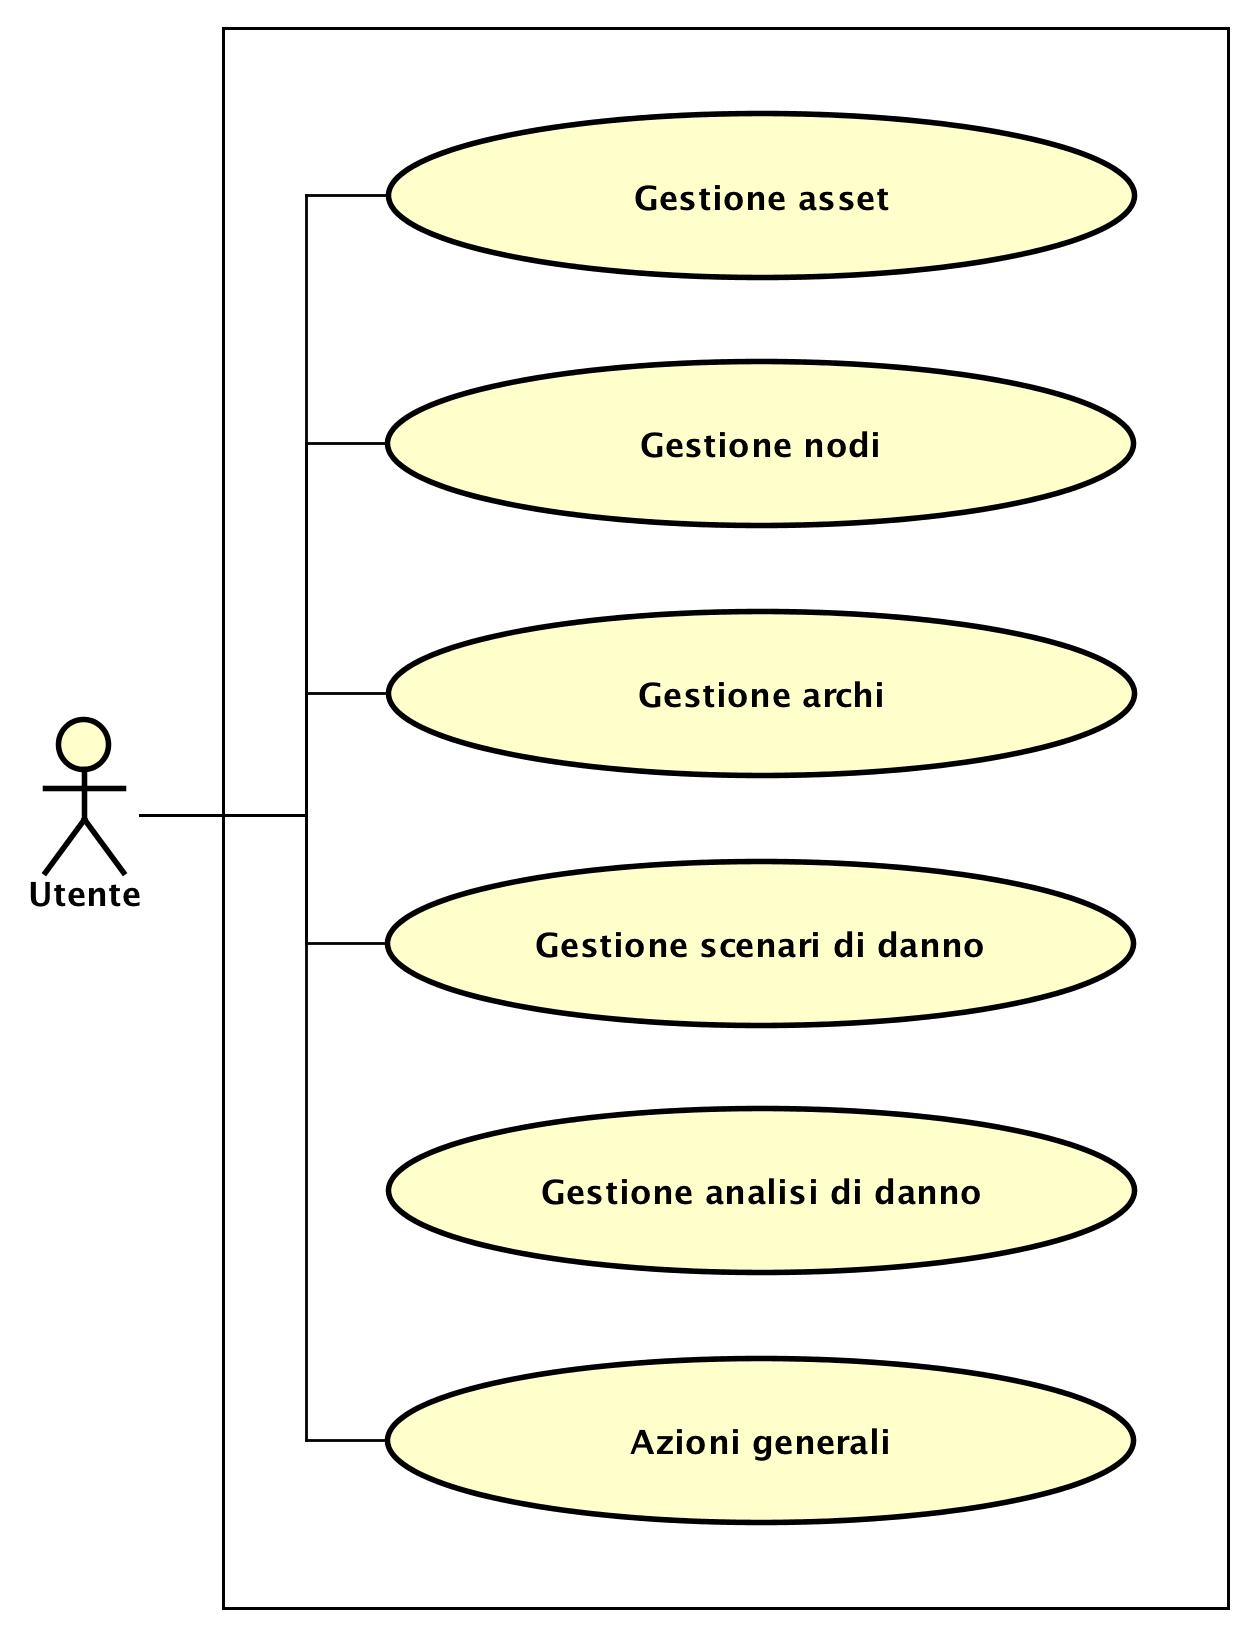
\includegraphics[width=\textwidth]{{img/uc00}.png}
		\caption{Panoramica dei casi d'uso - Generale}
	\end{figure}
	\begin{figure}[H]
		\centering
		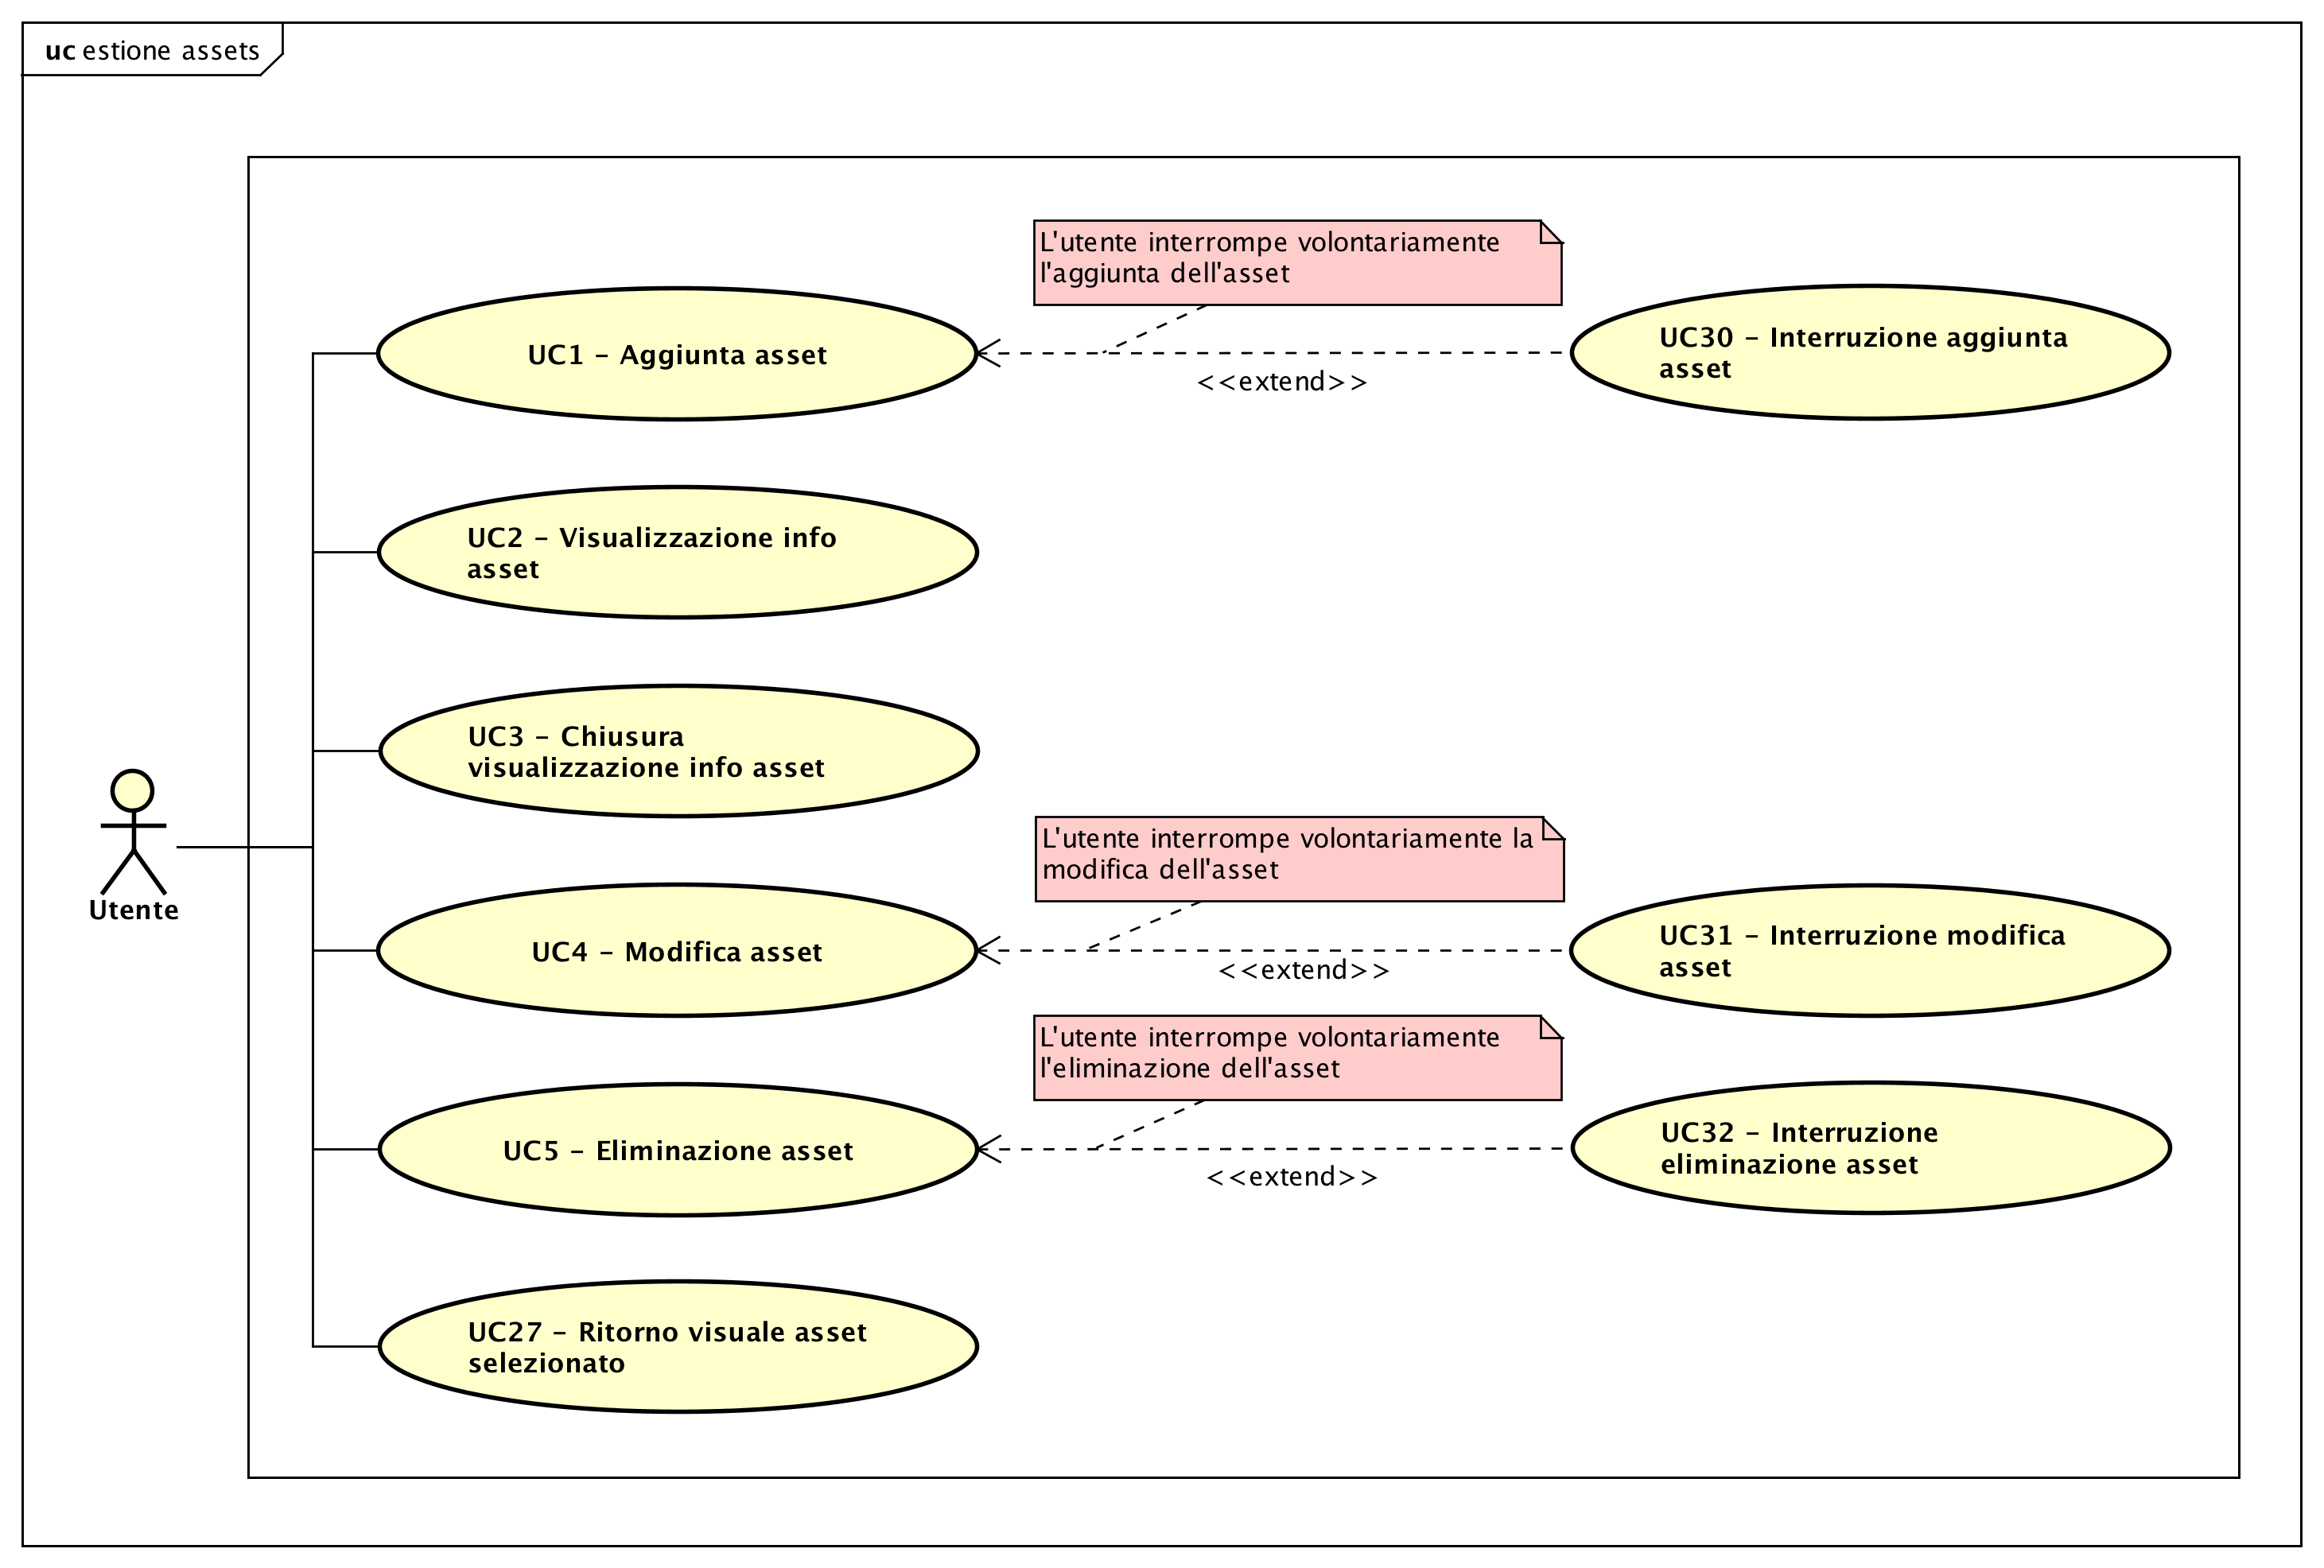
\includegraphics[width=\textwidth]{{img/uc0.1}.png}
		\caption{Panoramica dei casi d'uso - Gestione asset}
	\end{figure}
	\begin{figure}[H]
		\centering
		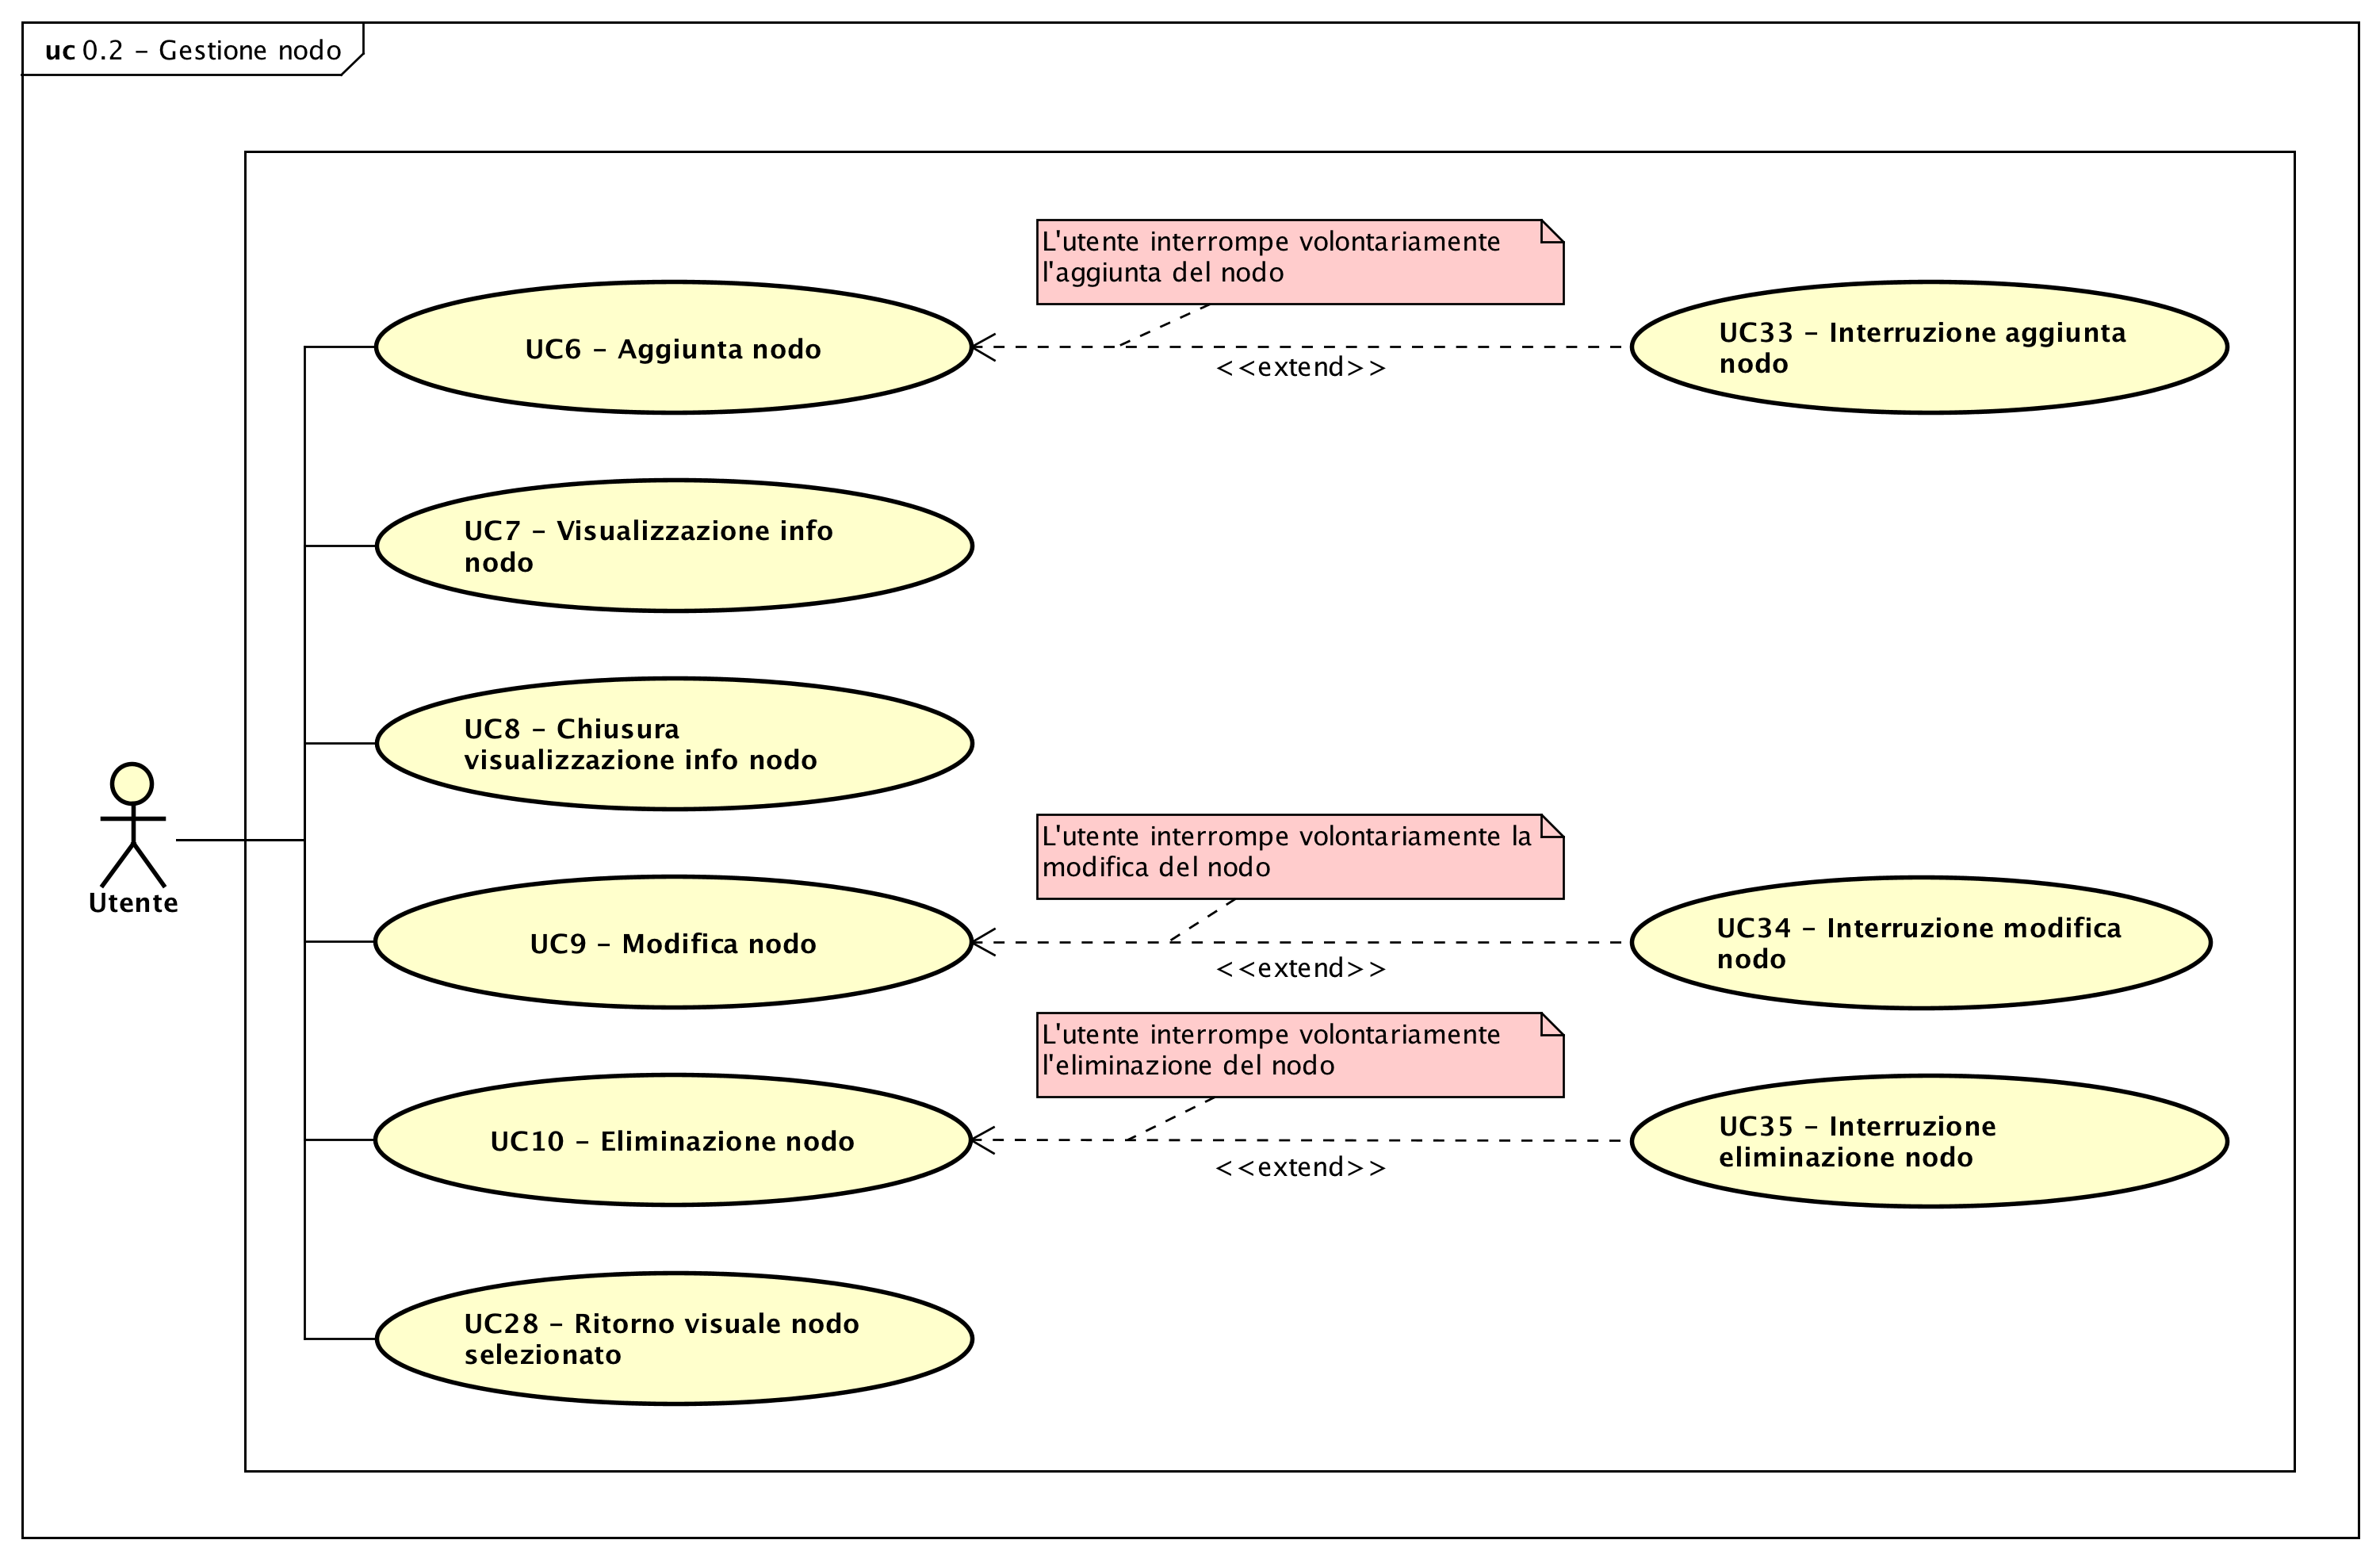
\includegraphics[width=\textwidth]{{img/uc0.2}.png}
		\caption{Panoramica dei casi d'uso - Gestione nodi}
	\end{figure}
	\begin{figure}[H]
		\centering
		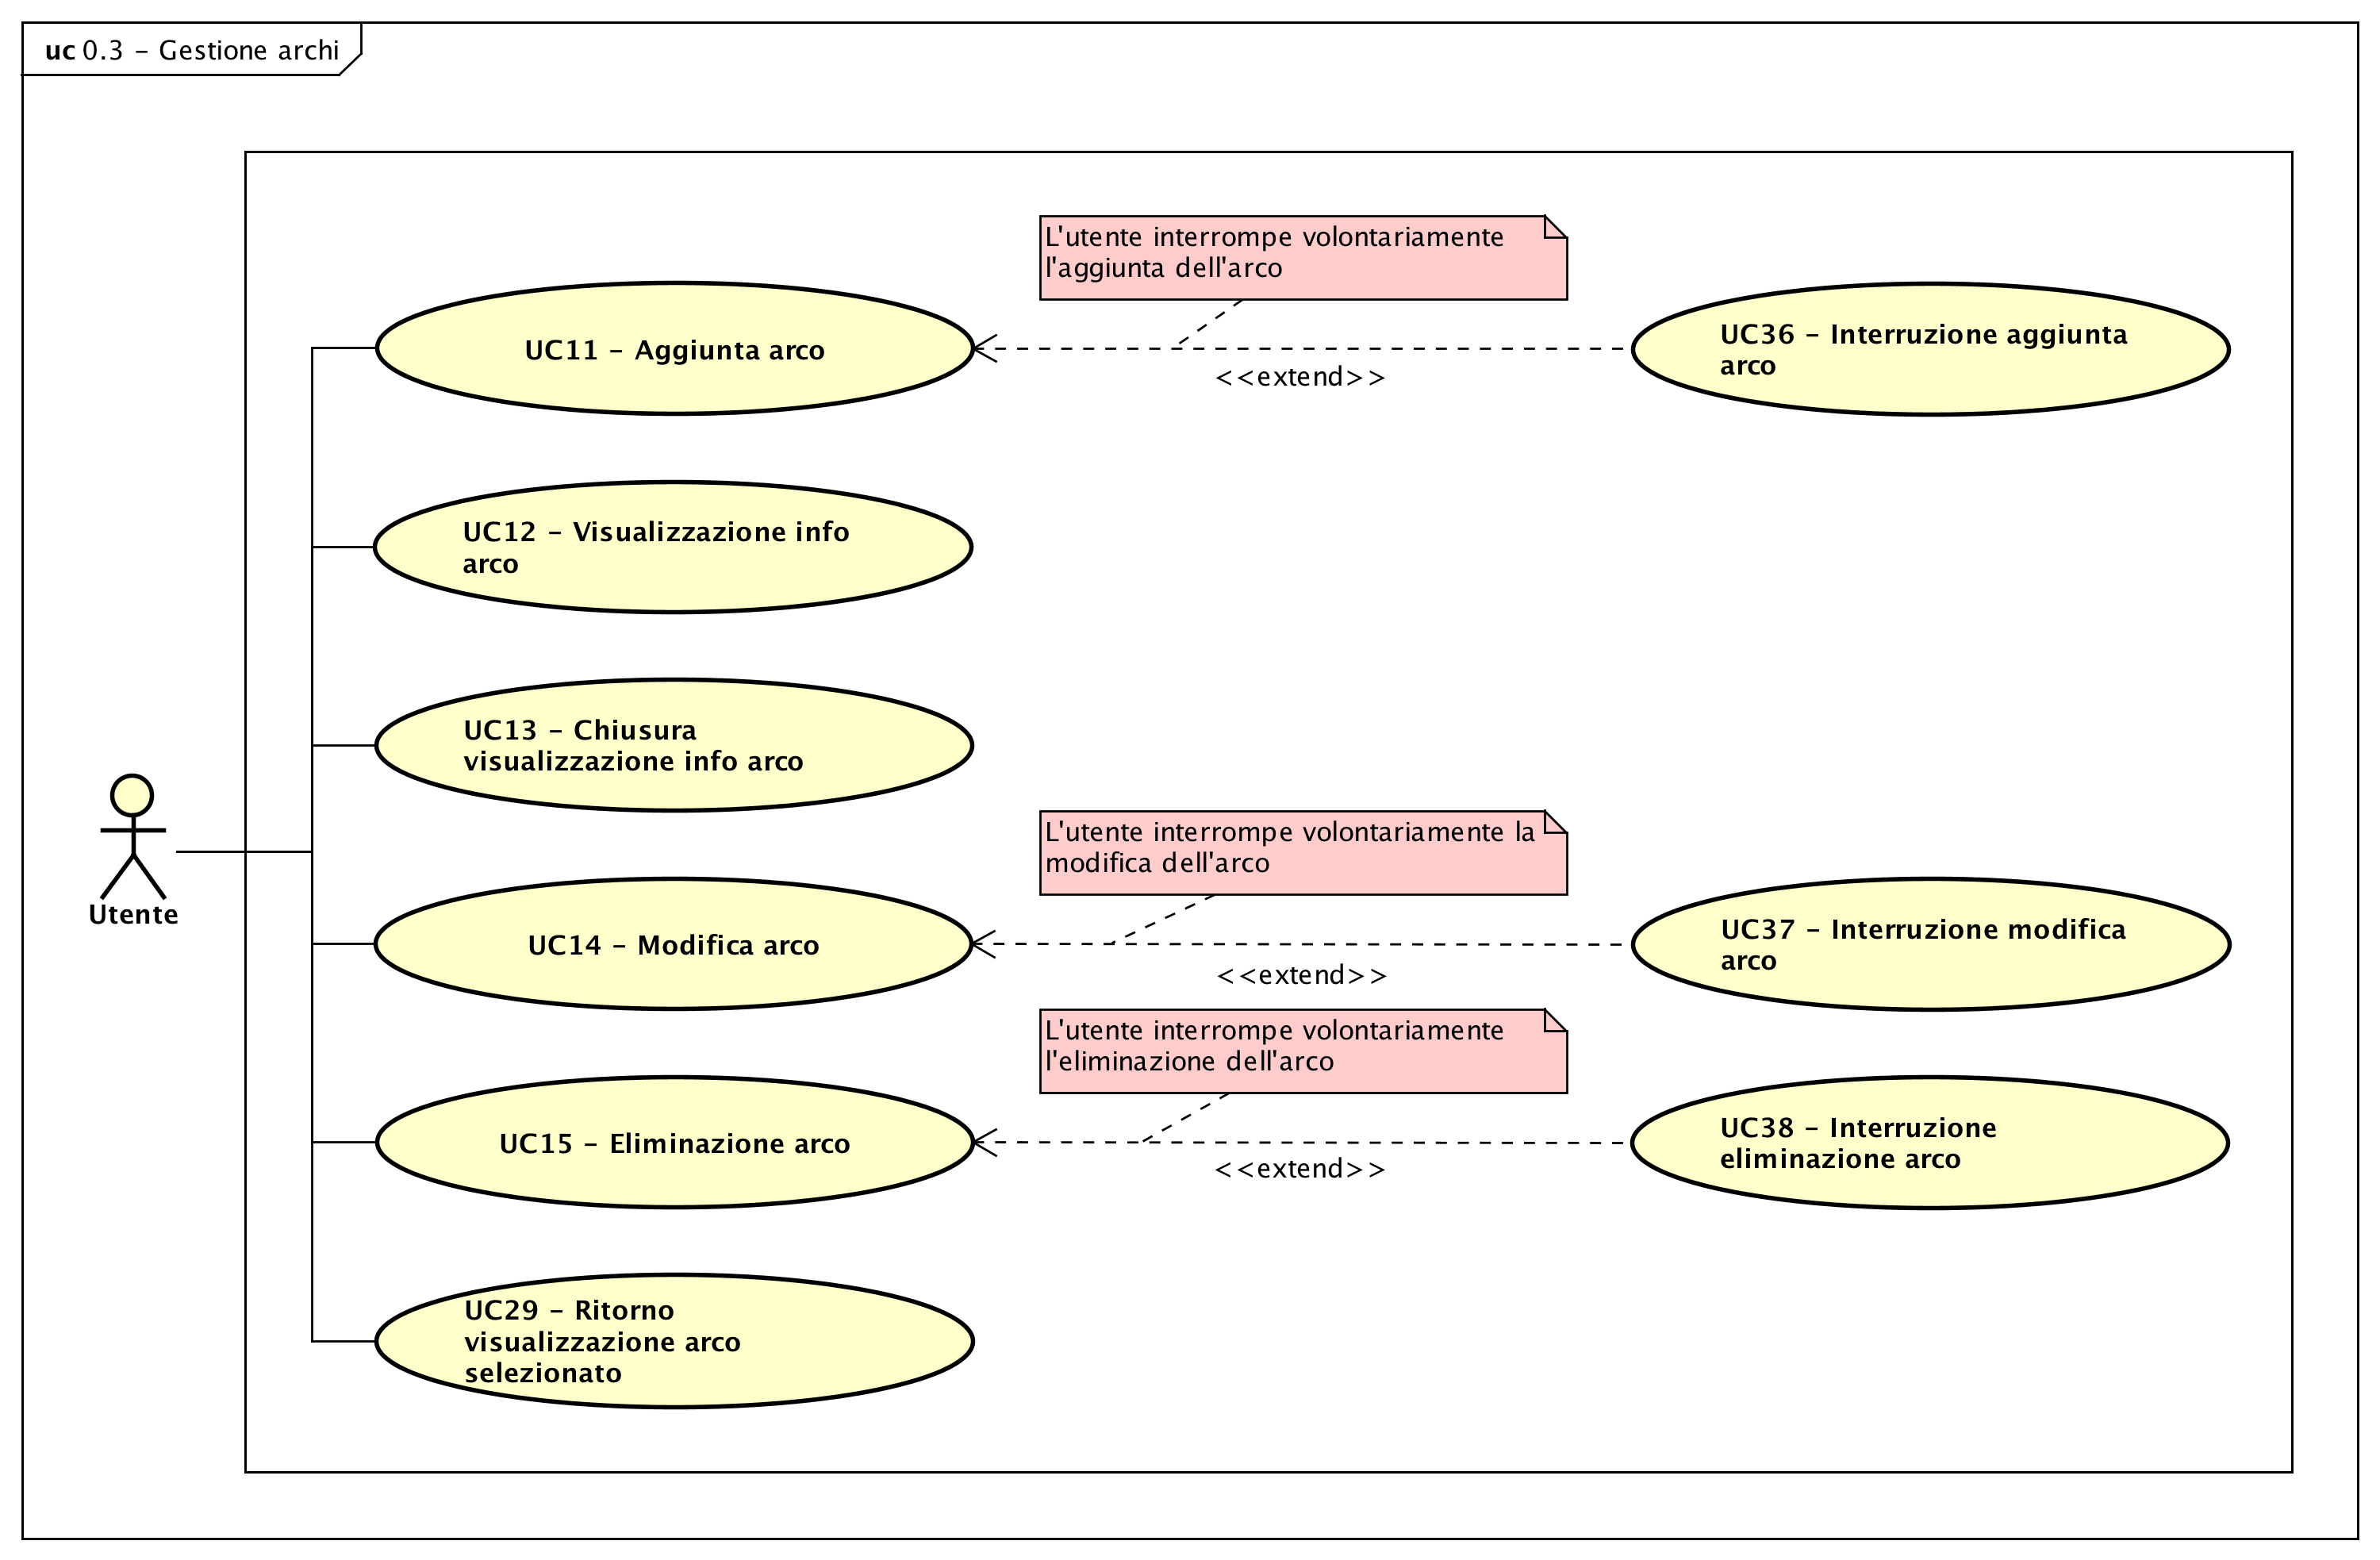
\includegraphics[width=\textwidth]{{img/uc0.3}.png}
		\caption{Panoramica dei casi d'uso - Gestione archi}
	\end{figure}
	\begin{figure}[H]
		\centering
		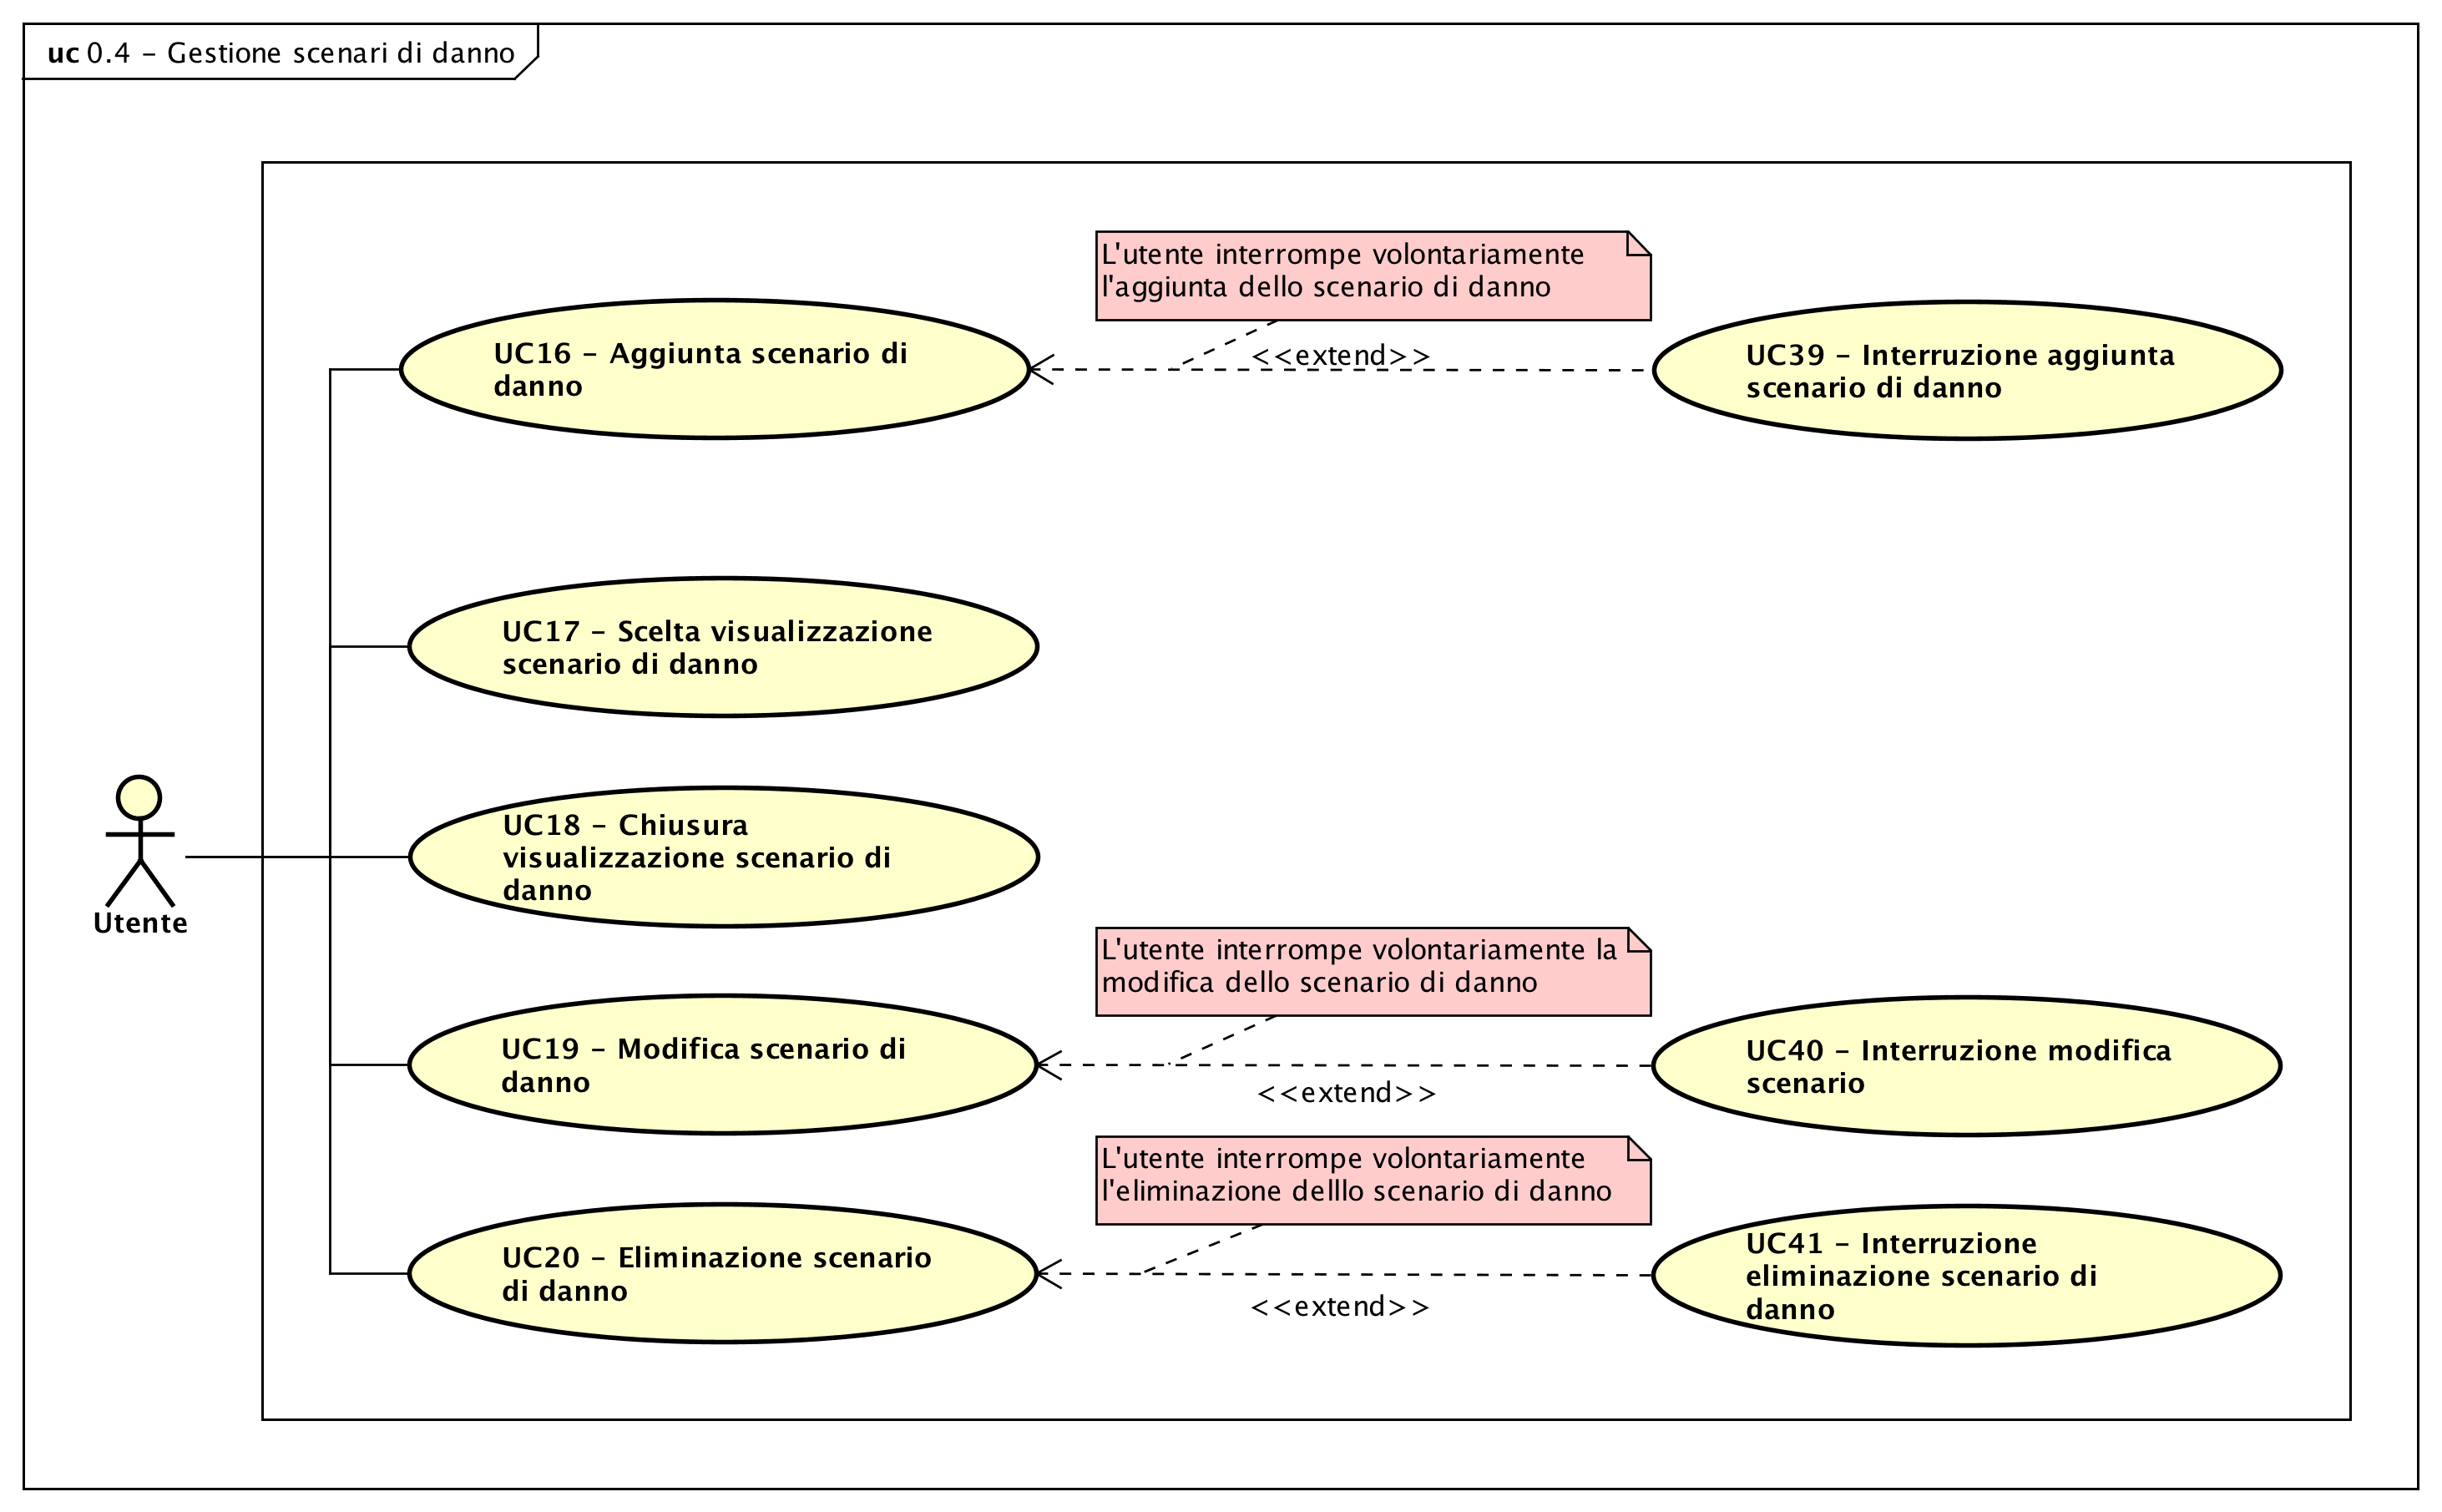
\includegraphics[width=\textwidth]{{img/uc0.4}.png}
		\caption{Panoramica dei casi d'uso - Gestione scenari di danno}
	\end{figure}
	\begin{figure}[H]
		\centering
		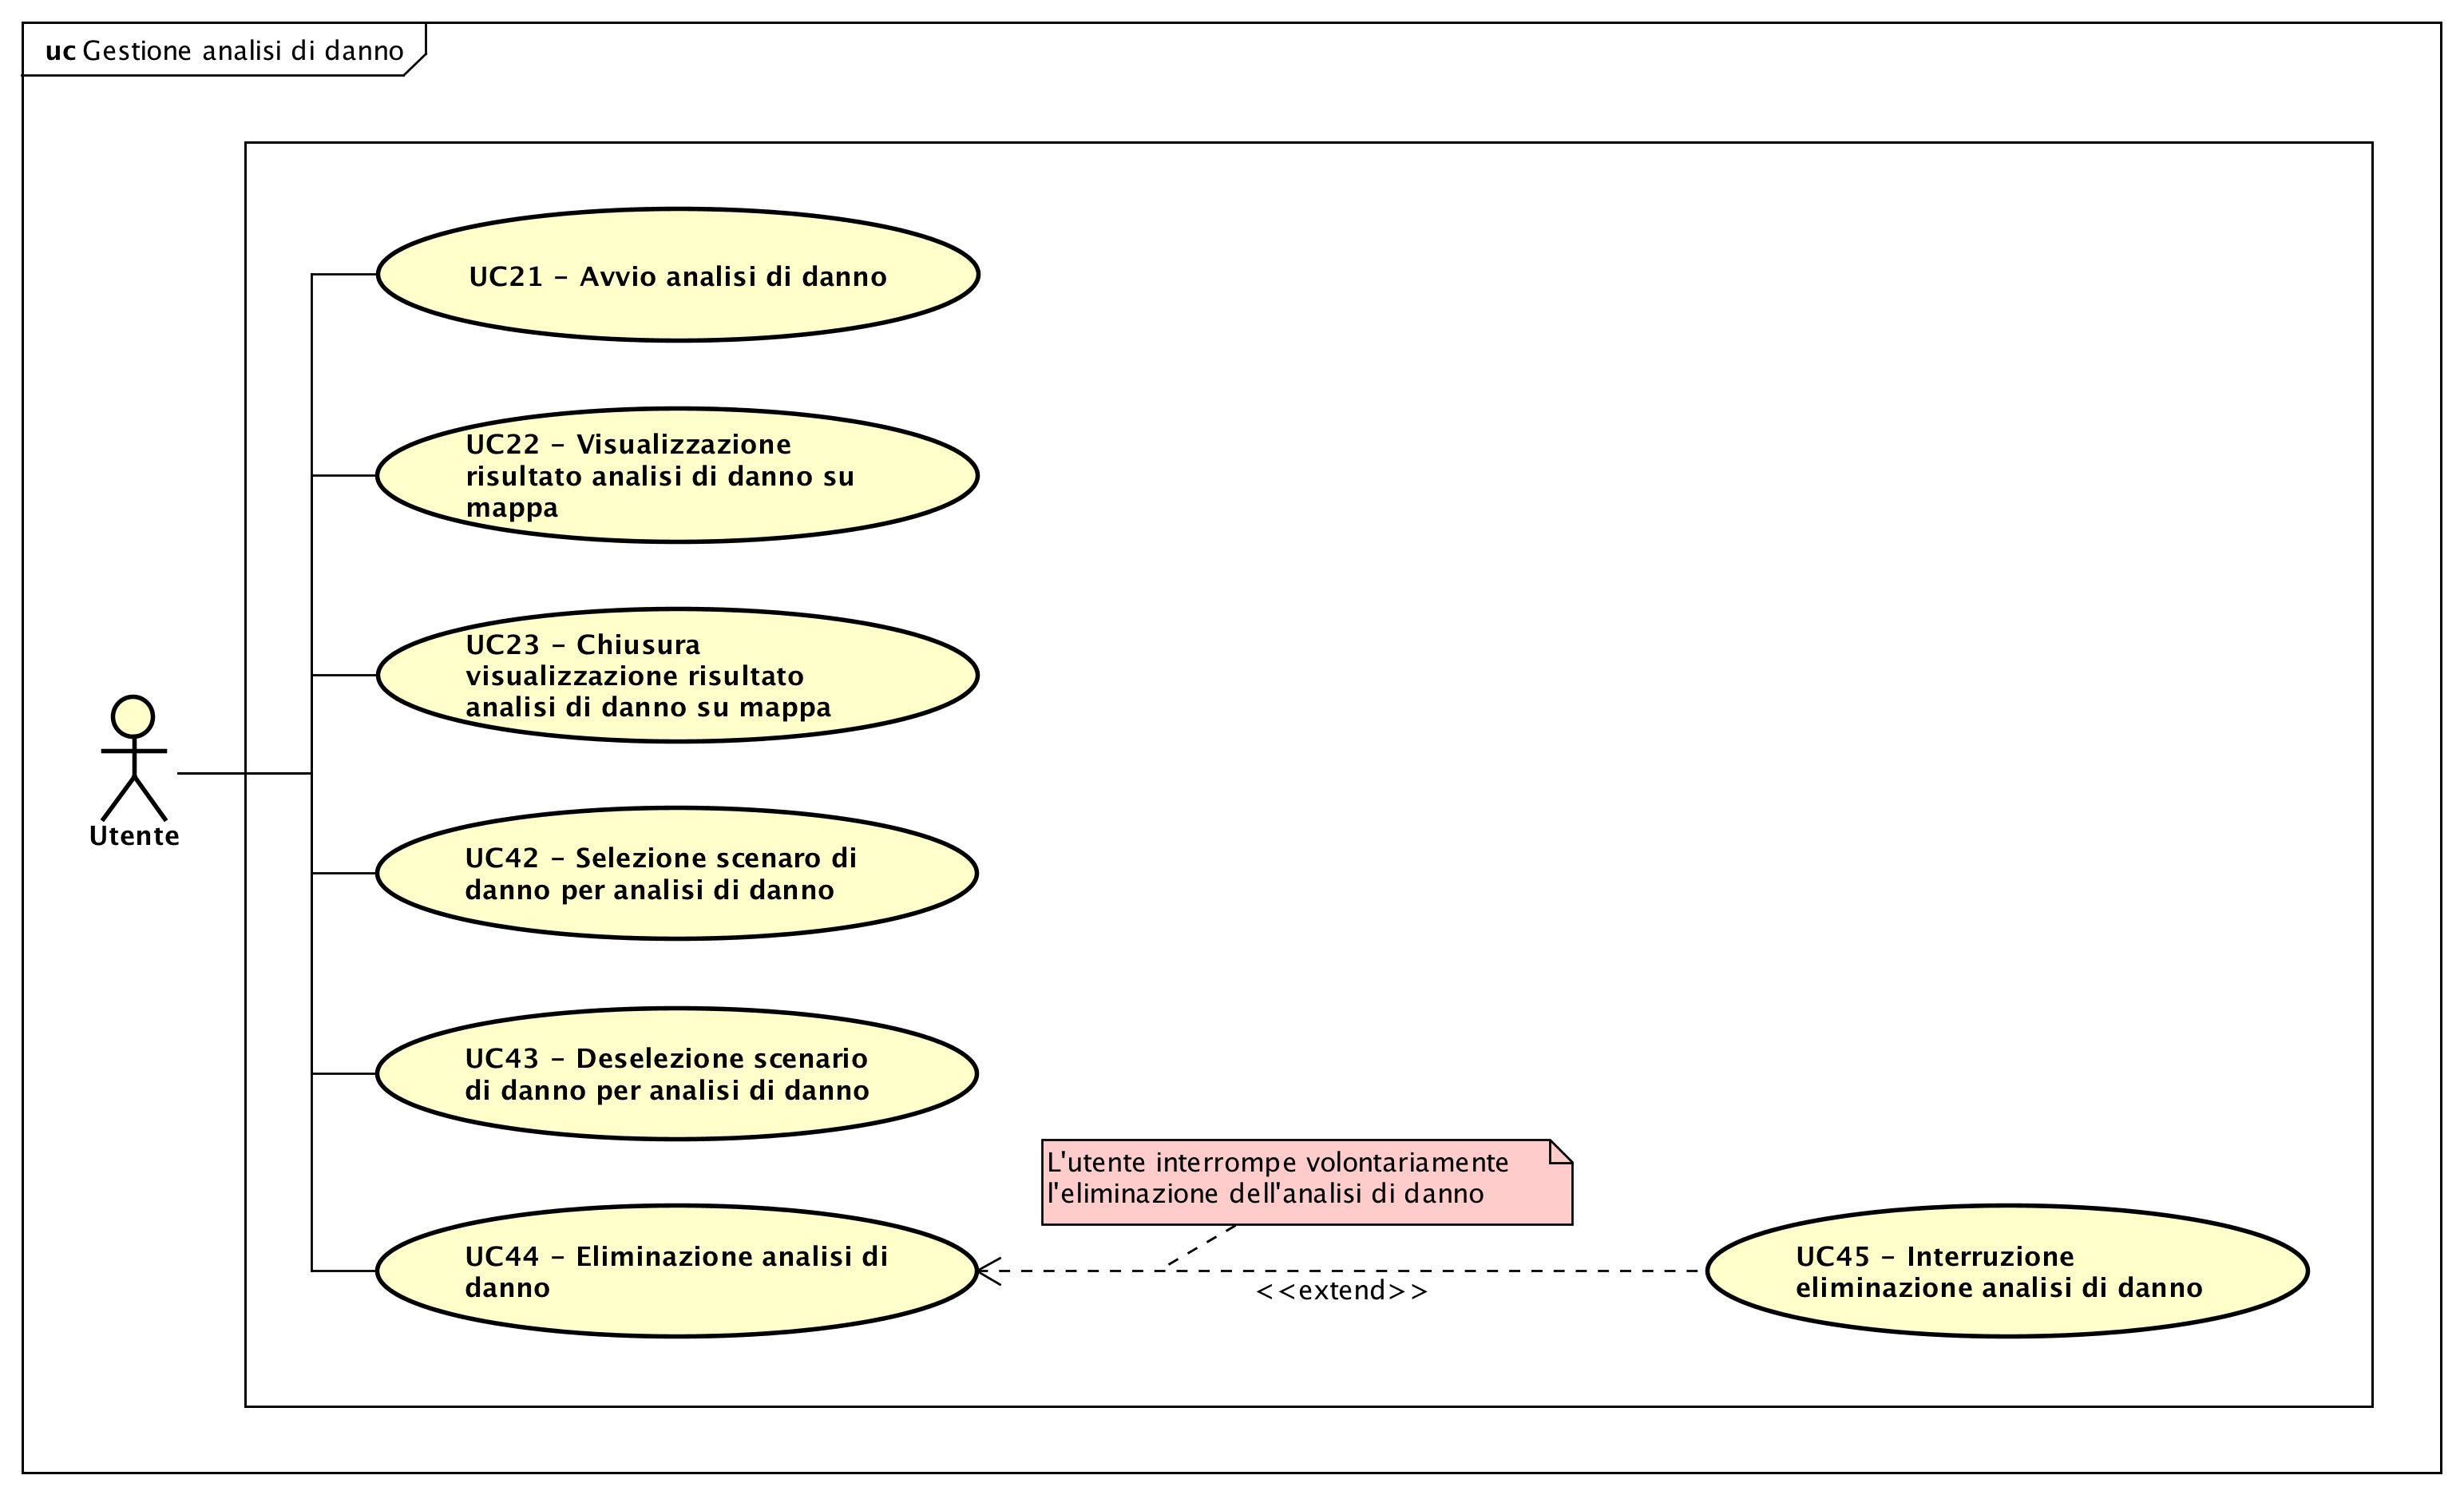
\includegraphics[width=\textwidth]{{img/uc0.5}.png}
		\caption{Panoramica dei casi d'uso - Gestione analisi di danno}
	\end{figure}
	\begin{figure}[H]
		\centering
		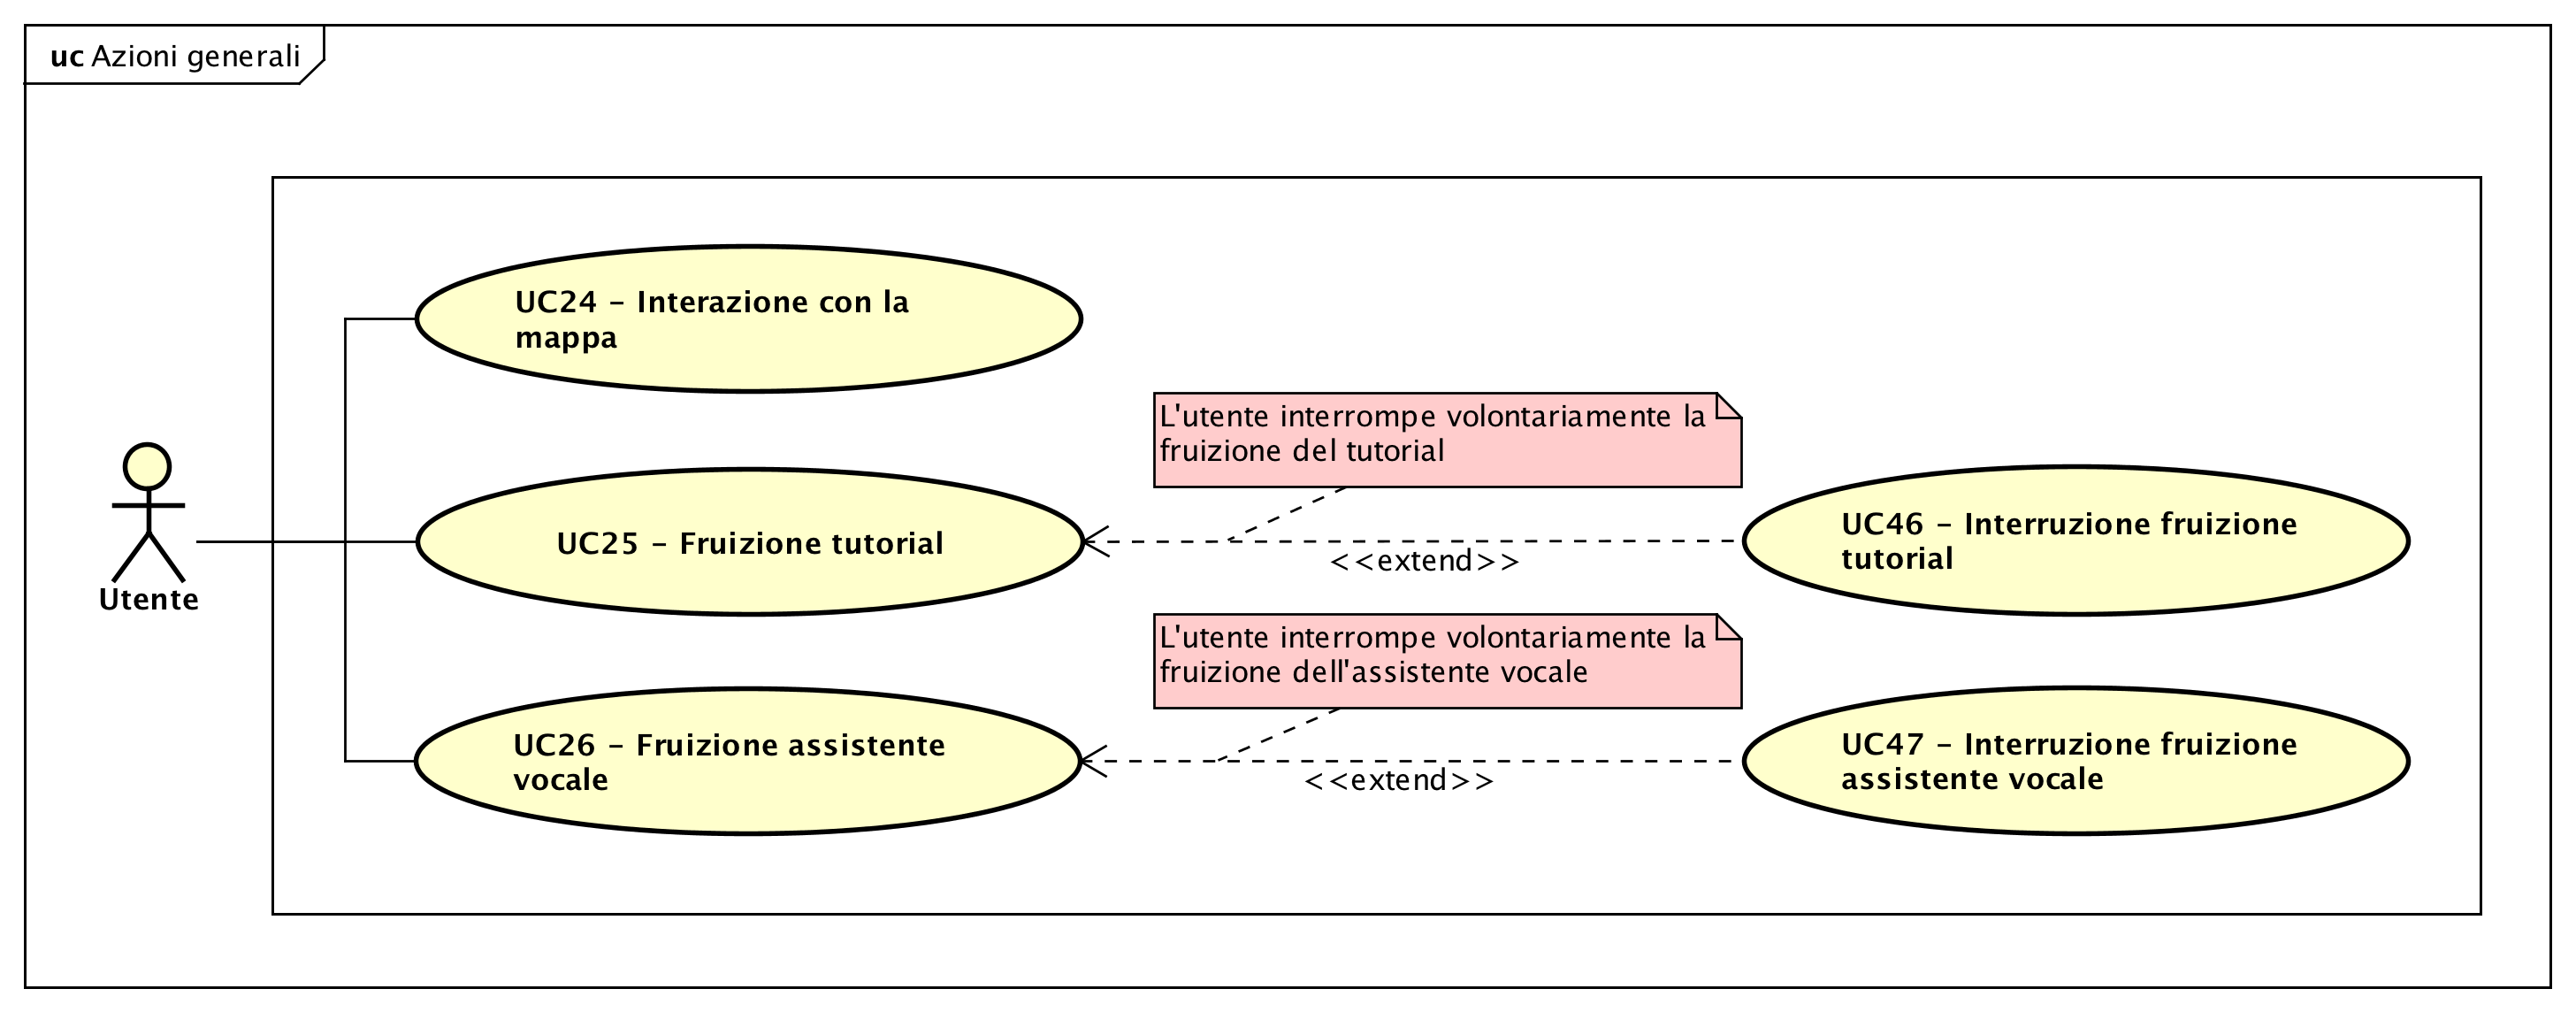
\includegraphics[width=\textwidth]{{img/uc0.6}.png}
		\caption{Panoramica dei casi d'uso - Azioni generali}
	\end{figure}
\subsection{UC1 - Aggiunta asset} 
\label{sssec:UC1} 
\begin{figure}[H] 
	\centering 
	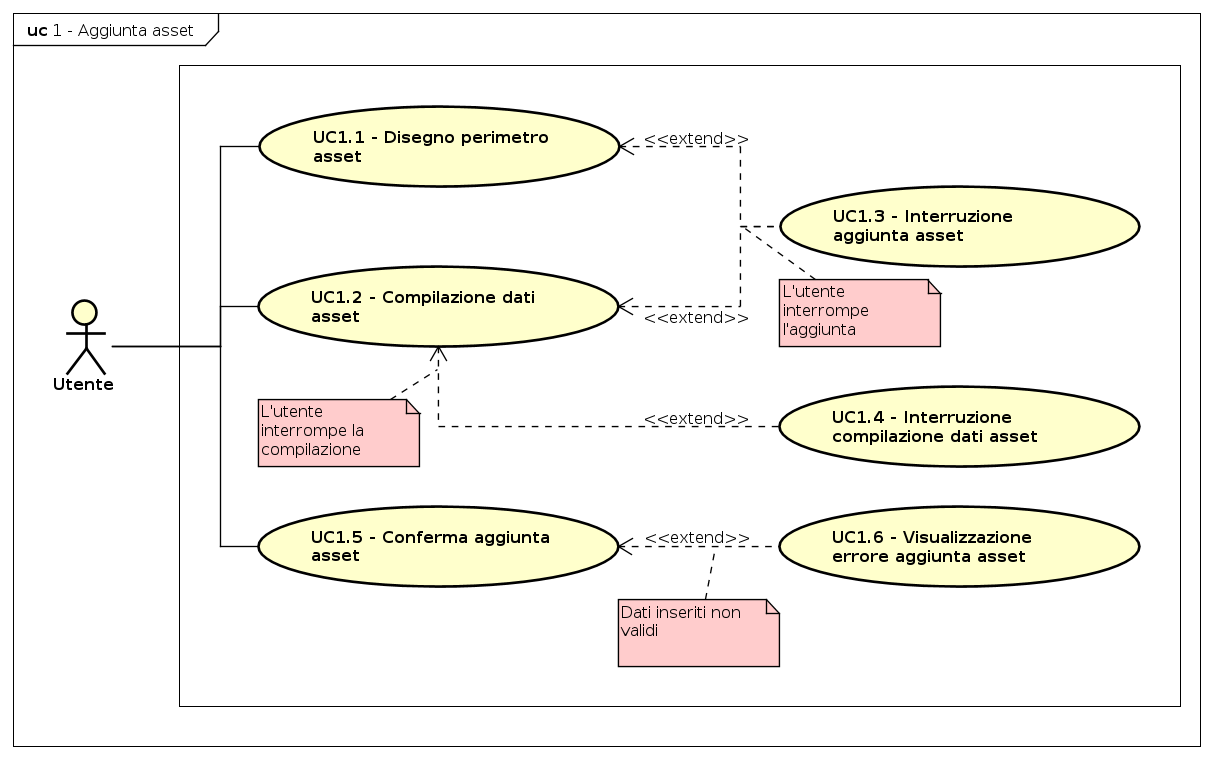
\includegraphics[width=\textwidth]{{img/uc1}.png} 
	\caption{UC1 - Aggiunta asset}
\end{figure}
\def\arraystretch{1.5}
\rowcolors{2}{D}{P}
\begin{tabularx}{\textwidth}{l|p{0.7\textwidth}}
	\rowcolor{I} \multicolumn{2}{c}{\color{white}\textbf{UC1 - Aggiunta asset}} \\
	\toprule
	\endhead
	\textbf{Attori} & Utente\\
	\textbf{Descrizione} & l'utente aggiunge un asset\\
	\textbf{Pre-condizione} & l'utente ha aperto l'applicazione\\
	\textbf{Post-condizione} & un nuovo asset è stato aggiunto ed è visualizzabile sulla mappa; l'utente visualizza un messaggio che comunica la corretta esecuzione dell'operazione; l'area informativa rimane impostata sull'asset appena inserito; la posizione e il livello di ingrandimento della mappa rimangono invariati\\
	\textbf{Scenario principale} & \vspace{-1.2em}\begin{enumerate}[leftmargin=*,noitemsep,nosep]
		\item \nameref{sssec:UC1.1};
		\item \nameref{sssec:UC1.2};
		\item \nameref{sssec:UC1.4}.
	\end{enumerate}\\
	\textbf{Estensioni} & \vspace{-1.2em}\begin{itemize}[leftmargin=*,noitemsep,nosep]
		\item \nameref{sssec:UC30}: l’utente interrompe volontariamente l’aggiunta dell’asset
	\end{itemize}\\
	\textbf{Scenari alternativi} & \vspace{-1.2em}\begin{itemize}[leftmargin=*,noitemsep,nosep]
		\item \nameref{sssec:UC1.3};
		\item \nameref{sssec:UC1.5}.
	\end{itemize}\\
	%\textbf{Generalizzazioni} &  \\
	\bottomrule
\end{tabularx}
\subsection{UC1.1 - Disegno perimetro asset} 
\label{sssec:UC1.1} 
\begin{figure}[H] 
	\centering 
	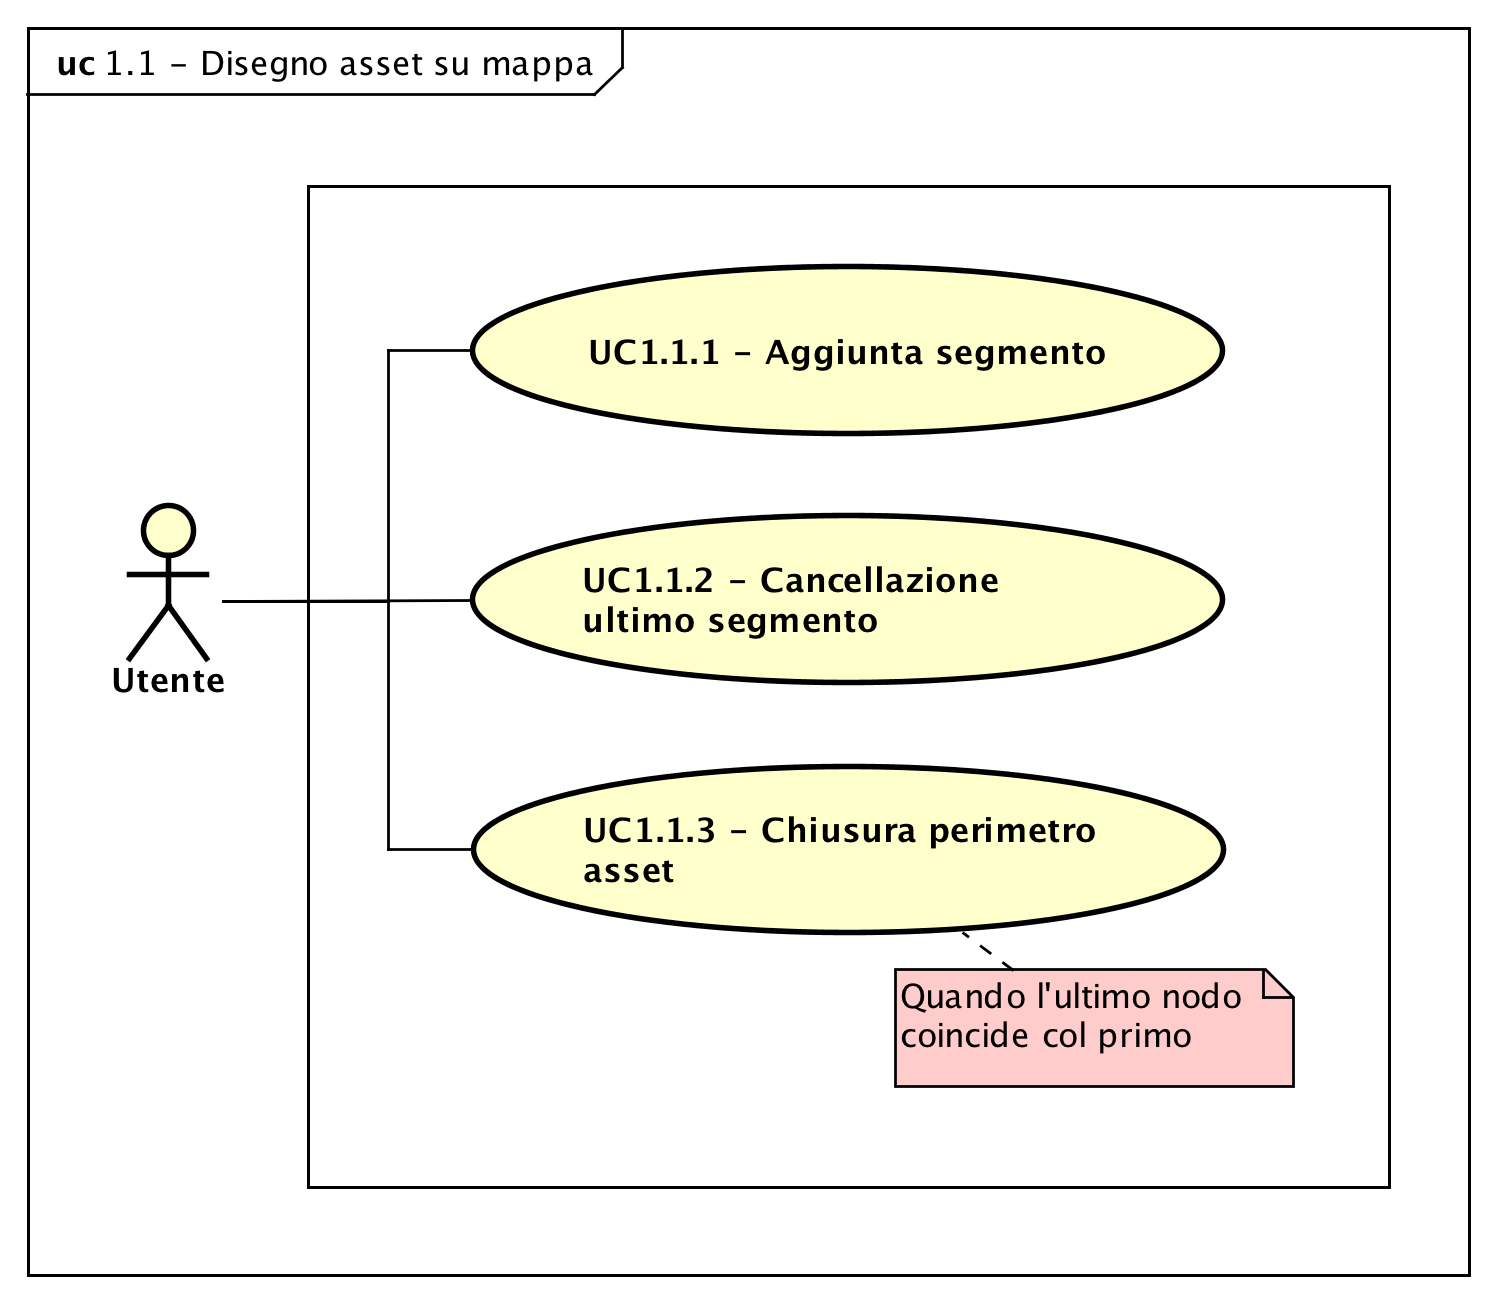
\includegraphics[scale=0.5]{{img/uc1.1}.png} 
	\caption{UC1.1 - Disegno perimetro asset}
\end{figure}
\def\arraystretch{1.5}
\rowcolors{2}{D}{P}
\begin{tabularx}{\textwidth}{l|p{0.7\textwidth}}
	\rowcolor{I} \multicolumn{2}{c}{\color{white}\textbf{UC1.1 - Disegno perimetro asset}} \\
	\toprule
	\endhead
	\textbf{Attori} & Utente\\
	\textbf{Descrizione} & l'utente disegna su mappa il perimetro dell'asset\\
	\textbf{Pre-condizione} & il sistema offre la possibilità di disegnare su mappa il perimetro dell'asset\\
	\textbf{Post-condizione} & il perimetro dell'asset è stato disegnato e viene visualizzato sulla mappa; l'utente può procedere alla compilazione dei restanti dati dell'asset nell'area informativa\\
	\textbf{Scenario principale} & \vspace{-1.2em}\begin{enumerate}[leftmargin=*,noitemsep,nosep]
		\item \nameref{sssec:UC1.1.1};
		\item \nameref{sssec:UC1.1.2};
		\item \nameref{sssec:UC1.1.3}.
	\end{enumerate}\\
	%\textbf{Generalizzazioni} &  \\
	\bottomrule
\end{tabularx}
\subsection{UC1.1.1 - Aggiunta segmento} 
\label{sssec:UC1.1.1} 
\def\arraystretch{1.5}
\rowcolors{2}{D}{P}
\begin{tabularx}{\textwidth}{l|p{0.7\textwidth}}
	\rowcolor{I} \multicolumn{2}{c}{\color{white}\textbf{UC1.1.1 - Aggiunta segmento}} \\
	\toprule
	\endhead
	\textbf{Attori} & Utente\\
	\textbf{Descrizione} & l'utente aggiunge un segmento al perimetro dell'asset che sta disegnando\\
	\textbf{Pre-condizione} & il sistema offre la possibilità di aggiungere un segmento al perimetro dell'asset\\
	\textbf{Post-condizione} & l'utente ha aggiunto un segmento al perimetro dell'asset che sta disegnando; il segmento viene visualizzato sulla mappa\\
	\textbf{Scenario principale} & \vspace{-1.2em}\begin{enumerate}[leftmargin=*,noitemsep,nosep]
		\item \nameref{sssec:UC1.1.1}.
	\end{enumerate}\\
	%\textbf{Generalizzazioni} &  \\
	\bottomrule
\end{tabularx}
\subsection{UC1.1.2 - Cancellazione ultimo segmento} 
\label{sssec:UC1.1.2} 
\def\arraystretch{1.5}
\rowcolors{2}{D}{P}
\begin{tabularx}{\textwidth}{l|p{0.7\textwidth}}
	\rowcolor{I} \multicolumn{2}{c}{\color{white}\textbf{UC1.1.2 - Cancellazione ultimo segmento}} \\
	\toprule
	\endhead
	\textbf{Attori} & Utente\\
	\textbf{Descrizione} & l'utente cancella l'ultimo segmento del perimetro dell'asset che sta disegnando\\
	\textbf{Pre-condizione} & l'utente sta disegnando il perimetro di un asset; è stato disegnato almeno un segmento\\
	\textbf{Post-condizione} & l'utente ha cancellato l'ultimo segmento del perimetro dell'asset che sta disegnando; l'ultimo segmento non è più visualizzato sulla mappa\\
	\textbf{Scenario principale} & \vspace{-1.2em}\begin{enumerate}[leftmargin=*,noitemsep,nosep]
		\item \nameref{sssec:UC1.1.2}.
	\end{enumerate}\\
	%\textbf{Generalizzazioni} &  \\
	\bottomrule
\end{tabularx}
\subsection{UC1.1.3 - Chiusura perimetro asset} 
\label{sssec:UC1.1.3} 
\def\arraystretch{1.5}
\rowcolors{2}{D}{P}
\begin{tabularx}{\textwidth}{l|p{0.7\textwidth}}
	\rowcolor{I} \multicolumn{2}{c}{\color{white}\textbf{UC1.1.3 - Chiusura perimetro asset}} \\
	\toprule
	\endhead
	\textbf{Attori} & Utente\\
	\textbf{Descrizione} & l'utente termina di disegnare il perimetro di un asset, facendo coincidere ultimo e primo nodo\\
	\textbf{Pre-condizione} & il sistema offre la possibilità di disegnare il perimetro di un asset; l'utente ha disegnato almeno due segmenti\\
	\textbf{Post-condizione} & l'utente ha terminato di disegnare il perimetro di un asset, che viene visualizzato sulla mappa; l'utente può continuare a procedere con l'inserimento degli altri dati dell'asset sull'area informativa\\
	\textbf{Scenario principale} & \vspace{-1.2em}\begin{enumerate}[leftmargin=*,noitemsep,nosep]
		\item \nameref{sssec:UC1.1.3}.
	\end{enumerate}\\
	%\textbf{Generalizzazioni} &  \\
	\bottomrule
\end{tabularx}
\subsection{UC1.2 - Compilazione dati asset} 
\label{sssec:UC1.2} 
\begin{figure}[H] 
	\centering 
	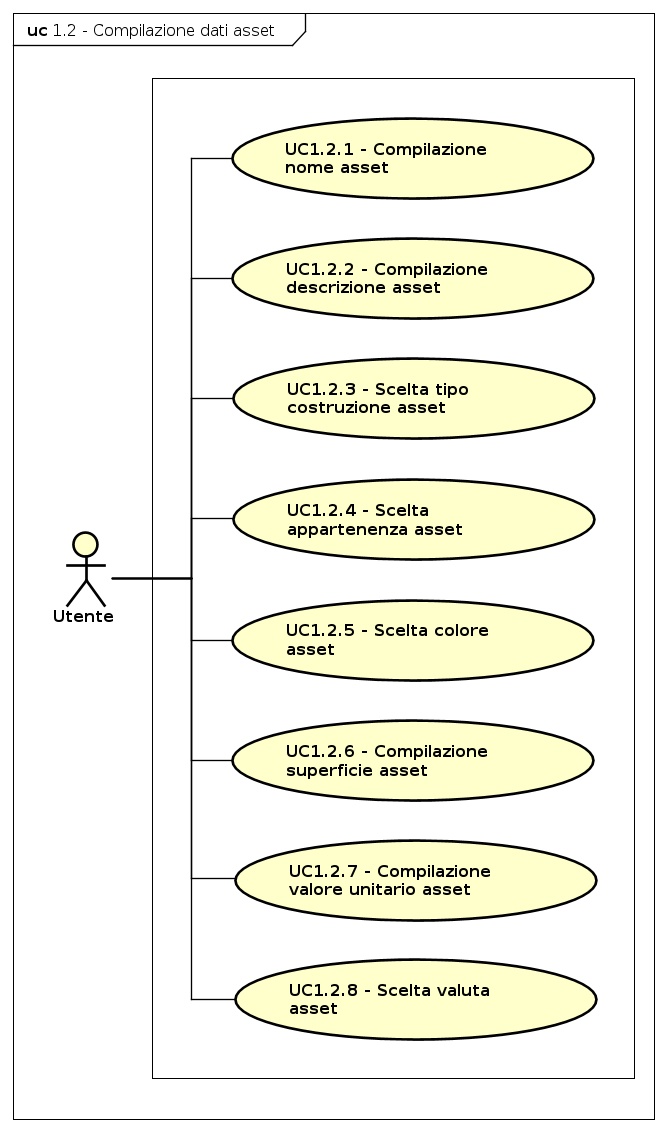
\includegraphics[scale=0.5]{{img/uc1.2}.png} 
	\caption{UC1.2 - Compilazione dati asset}
\end{figure}
\def\arraystretch{1.5}
\rowcolors{2}{D}{P}
\begin{tabularx}{\textwidth}{l|p{0.7\textwidth}}
	\rowcolor{I} \multicolumn{2}{c}{\color{white}\textbf{UC1.2 - Compilazione dati asset}} \\
	\toprule
	\endhead
	\textbf{Attori} & Utente\\
	\textbf{Descrizione} & l'utente compila i dati dell'asset che sta aggiungendo\\
	\textbf{Pre-condizione} & il sistema offre la possibilità di compilare i dati dell'asset\\
	\textbf{Post-condizione} & l'utente ha compilato i dati dell'asset che sta aggiungendo e viene riportato alla schermata di aggiunta dell'asset\\
	\textbf{Scenario principale} & \vspace{-1.2em}\begin{enumerate}[leftmargin=*,noitemsep,nosep]
		\item \nameref{sssec:UC1.2.1};
		\item \nameref{sssec:UC1.2.2};
		\item \nameref{sssec:UC1.2.3};
		\item \nameref{sssec:UC1.2.4};
		\item \nameref{sssec:UC1.2.5};
		\item \nameref{sssec:UC1.2.6};
		\item \nameref{sssec:UC1.2.7}.
	\end{enumerate}\\
	\textbf{Estensioni} & \vspace{-1.2em}\begin{itemize}[leftmargin=*,noitemsep,nosep]
		\item \nameref{sssec:UC1.3}: l’utente interrompe volontariamente la compilazione dei dati dell'asset
	\end{itemize}\\
	%\textbf{Generalizzazioni} &  \\
	\bottomrule
\end{tabularx}
\subsection{UC1.2.1 - Compilazione nome asset} 
\label{sssec:UC1.2.1} 
\def\arraystretch{1.5}
\rowcolors{2}{D}{P}
\begin{tabularx}{\textwidth}{l|p{0.7\textwidth}}
	\rowcolor{I} \multicolumn{2}{c}{\color{white}\textbf{UC1.2.1 - Compilazione nome asset}} \\
	\toprule
	\endhead
	\textbf{Attori} & Utente\\
	\textbf{Descrizione} & l'utente compila il nome dell'asset\\
	\textbf{Pre-condizione} & il sistema offre la possibilità di compilare il nome dell'asset\\
	\textbf{Post-condizione} & l'utente ha compilato il nome dell'asset e può visualizzare il nome appena compilato sull'area informativa\\
	\textbf{Scenario principale} & \vspace{-1.2em}\begin{enumerate}[leftmargin=*,noitemsep,nosep]
		\item \nameref{sssec:UC1.2.1}.
	\end{enumerate}\\
	%\textbf{Generalizzazioni} &  \\
	\bottomrule
\end{tabularx}
\subsection{UC1.2.2 - Compilazione descrizione asset} 
\label{sssec:UC1.2.2} 
\def\arraystretch{1.5}
\rowcolors{2}{D}{P}
\begin{tabularx}{\textwidth}{l|p{0.7\textwidth}}
	\rowcolor{I} \multicolumn{2}{c}{\color{white}\textbf{UC1.2.2 - Compilazione descrizione asset}} \\
	\toprule
	\endhead
	\textbf{Attori} & Utente\\
	\textbf{Descrizione} & l'utente compila la descrizione dell'asset\\
	\textbf{Pre-condizione} & il sistema offre la possibilità di compilare la descrizione dell'asset\\
	\textbf{Post-condizione} & l'utente ha compilato la descrizione dell'asset e può visualizzare la descrizione appena compilata sull'area informativa\\
	\textbf{Scenario principale} & \vspace{-1.2em}\begin{enumerate}[leftmargin=*,noitemsep,nosep]
		\item \nameref{sssec:UC1.2.2}.
	\end{enumerate}\\
	%\textbf{Generalizzazioni} &  \\
	\bottomrule
\end{tabularx}
\subsection{UC1.2.3 - Scelta tipo costruzione asset} 
\label{sssec:UC1.2.3} 
\def\arraystretch{1.5}
\rowcolors{2}{D}{P}
\begin{tabularx}{\textwidth}{l|p{0.7\textwidth}}
	\rowcolor{I} \multicolumn{2}{c}{\color{white}\textbf{UC1.2.3 - Scelta tipo costruzione asset}} \\
	\toprule
	\endhead
	\textbf{Attori} & Utente\\
	\textbf{Descrizione} & l'utente sceglie il tipo di costruzione dell'asset\\
	\textbf{Pre-condizione} & il sistema offre la possibilità di scegliere il tipo di costruzione dell'asset\\
	\textbf{Post-condizione} & l'utente ha scelto il tipo di costruzione dell'asset e può visualizzare il tipo appena scelto sull'area informativa\\
	\textbf{Scenario principale} & \vspace{-1.2em}\begin{enumerate}[leftmargin=*,noitemsep,nosep]
		\item \nameref{sssec:UC1.2.3}.
	\end{enumerate}\\
	%\textbf{Generalizzazioni} &  \\
	\bottomrule
\end{tabularx}
\subsection{UC1.2.4 - Scelta appartenenza asset} 
\label{sssec:UC1.2.4} 
\def\arraystretch{1.5}
\rowcolors{2}{D}{P}
\begin{tabularx}{\textwidth}{l|p{0.7\textwidth}}
	\rowcolor{I} \multicolumn{2}{c}{\color{white}\textbf{UC1.2.4 - Scelta appartenenza asset}} \\
	\toprule
	\endhead
	\textbf{Attori} & Utente\\
	\textbf{Descrizione} & l'utente sceglie a chi appartiene l'asset\\
	\textbf{Pre-condizione} & il sistema offre la possibilità di scegliere a chi appartiene l'asset\\
	\textbf{Post-condizione} & l'utente ha scelto a chi appartiene l'asset e può visualizzare l'appartenenza appena scelta sull'area informativa\\
	\textbf{Scenario principale} & \vspace{-1.2em}\begin{enumerate}[leftmargin=*,noitemsep,nosep]
		\item \nameref{sssec:UC1.2.4}.
	\end{enumerate}\\
	%\textbf{Generalizzazioni} &  \\
	\bottomrule
\end{tabularx}
\subsection{UC1.2.5 - Scelta colore asset} 
\label{sssec:UC1.2.5} 
\def\arraystretch{1.5}
\rowcolors{2}{D}{P}
\begin{tabularx}{\textwidth}{l|p{0.7\textwidth}}
	\rowcolor{I} \multicolumn{2}{c}{\color{white}\textbf{UC1.2.5 - Scelta colore asset}} \\
	\toprule
	\endhead
	\textbf{Attori} & Utente\\
	\textbf{Descrizione} & l'utente sceglie il colore dell'asset\\
	\textbf{Pre-condizione} & il sistema offre la possibilità di scegliere il colore dell'asset\\
	\textbf{Post-condizione} & l'utente ha scelto il colore dell'asset e può visualizzare il colore appena scelto sull'area informativa\\
	\textbf{Scenario principale} & \vspace{-1.2em}\begin{enumerate}[leftmargin=*,noitemsep,nosep]
		\item \nameref{sssec:UC1.2.5}.
	\end{enumerate}\\
	%\textbf{Generalizzazioni} &  \\
	\bottomrule
\end{tabularx}
\subsection{UC1.2.6 - Compilazione superficie asset} 
\label{sssec:UC1.2.6} 
\def\arraystretch{1.5}
\rowcolors{2}{D}{P}
\begin{tabularx}{\textwidth}{l|p{0.7\textwidth}}
	\rowcolor{I} \multicolumn{2}{c}{\color{white}\textbf{UC1.2.6 - Compilazione superficie asset}} \\
	\toprule
	\endhead
	\textbf{Attori} & Utente\\
	\textbf{Descrizione} & l'utente compila la superficie dell'asset\\
	\textbf{Pre-condizione} & il sistema offre la possibilità di compilare la superficie dell'asset\\
	\textbf{Post-condizione} & l'utente ha compilato la superficie dell'asset e può visualizzare la superficie appena compilata sull'area informativa\\
	\textbf{Scenario principale} & \vspace{-1.2em}\begin{enumerate}[leftmargin=*,noitemsep,nosep]
		\item \nameref{sssec:UC1.2.6}.
	\end{enumerate}\\
	%\textbf{Generalizzazioni} &  \\
	\bottomrule
\end{tabularx}
\subsection{UC1.2.7 - Compilazione valore unitario asset} 
\label{sssec:UC1.2.7} 
\def\arraystretch{1.5}
\rowcolors{2}{D}{P}
\begin{tabularx}{\textwidth}{l|p{0.7\textwidth}}
	\rowcolor{I} \multicolumn{2}{c}{\color{white}\textbf{UC1.2.7 - Compilazione valore unitario asset}} \\
	\toprule
	\endhead
	\textbf{Attori} & Utente\\
	\textbf{Descrizione} & l'utente compila il valore unitario dell'asset\\
	\textbf{Pre-condizione} & il sistema offre la possibilità di compilare il valore unitario dell'asset\\
	\textbf{Post-condizione} & l'utente ha compilato il valore unitario dell'asset e può visualizzare il valore appena compilato sull'area informativa\\
	\textbf{Scenario principale} & \vspace{-1.2em}\begin{enumerate}[leftmargin=*,noitemsep,nosep]
		\item \nameref{sssec:UC1.2.7}.
	\end{enumerate}\\
	%\textbf{Generalizzazioni} &  \\
	\bottomrule
\end{tabularx}
\subsection{UC1.3 - Interruzione compilazione dati asset} 
\label{sssec:UC1.3} 
\def\arraystretch{1.5}
\rowcolors{2}{D}{P}
\begin{tabularx}{\textwidth}{l|p{0.7\textwidth}}
	\rowcolor{I} \multicolumn{2}{c}{\color{white}\textbf{UC1.3 - Interruzione compilazione dati asset}} \\
	\toprule
	\endhead
	\textbf{Attori} & Utente\\
	\textbf{Descrizione} & l'utente interrompe la compilazione dei dati dell'asset\\
	\textbf{Pre-condizione} & il sistema offre la possibilità di compilare i dati dell'asset\\
	\textbf{Post-condizione} & i dati dell'asset non sono stati compilati; l'utente viene riportato alla fase di disegno dell'asset\\
	\textbf{Scenario principale} & \vspace{-1.2em}\begin{enumerate}[leftmargin=*,noitemsep,nosep]
		\item \nameref{sssec:UC1.3}.
	\end{enumerate}\\
	%\textbf{Generalizzazioni} &  \\
	\bottomrule
\end{tabularx}
\subsection{UC1.4 - Conferma aggiunta asset} 
\label{sssec:UC1.4} 
\def\arraystretch{1.5}
\rowcolors{2}{D}{P}
\begin{tabularx}{\textwidth}{l|p{0.7\textwidth}}
	\rowcolor{I} \multicolumn{2}{c}{\color{white}\textbf{UC1.4 - Conferma aggiunta asset}} \\
	\toprule
	\endhead
	\textbf{Attori} & Utente\\
	\textbf{Descrizione} & l'utente conferma l'aggiunta dell'asset\\
	\textbf{Pre-condizione} & il sistema offre la possibilità di confermare l'aggiunta dell'asset\\
	\textbf{Post-condizione} & un nuovo asset è stato aggiunto ed è visualizzabile sulla mappa; l'utente visualizza un messaggio che comunica la corretta esecuzione dell'operazione; l'area informativa rimane impostata sull'asset appena inserito; la posizione e il livello di ingrandimento della mappa rimangono invariati\\
	\textbf{Scenario principale} & \vspace{-1.2em}\begin{enumerate}[leftmargin=*,noitemsep,nosep]
		\item \nameref{sssec:UC1.4}.
	\end{enumerate}\\
	\textbf{Estensioni} & \vspace{-1.2em}\begin{itemize}[leftmargin=*,noitemsep,nosep]
		\item \nameref{sssec:UC1.5}: dati inseriti non validi:
		\begin{itemize}
			\item nome vuoto; più lungo di 50 caratteri;
			inizia e/o finisce con uno spazio; contiene caratteri speciali
			\item descrizione vuota; più lunga di 5000
			caratteri; inizia e/o finisce con uno spazio; contiene caratteri
			speciali diversi dall'apostrofo;
			\item tipo di costruzione non scelto;
			\item appartenenza non scelta;
			\item colore non scelto;
			\item superficie (in mq) vuota; più lunga di
			5 cifre per la parte intera; più di 2 per la parte decimale;
			\item valore unitario (monetario) vuoto; più
			lungo di 20 cifre per la parte intera; più di 2 per la parte
			decimale;
			\item valuta non scelta.
		\end{itemize}
	\end{itemize}\\
	%\textbf{Generalizzazioni} &  \\
	\bottomrule
\end{tabularx}
\subsection{UC1.5 - Visualizzazione errore aggiunta asset} 
\label{sssec:UC1.5} 
\def\arraystretch{1.5}
\rowcolors{2}{D}{P}
\begin{tabularx}{\textwidth}{l|p{0.7\textwidth}}
	\rowcolor{I} \multicolumn{2}{c}{\color{white}\textbf{UC1.5 - Visualizzazione errore aggiunta asset}} \\
	\toprule
	\endhead
	\textbf{Attori} & Utente\\
	\textbf{Descrizione} & l'utente visualizza un errore relativo ai dati dell'asset compilati in modo errato\\
	\textbf{Pre-condizione} & l'utente sta tentando di inserire un nuovo asset\\
	\textbf{Post-condizione} & nessun nuovo asset inserito; l'utente visualizza un errore relativo ai dati dell'asset compilati in modo errato; l'utente viene riportato alla schermata di aggiunta asset\\
	\textbf{Scenario principale} & \vspace{-1.2em}\begin{enumerate}[leftmargin=*,noitemsep,nosep]
		\item \nameref{sssec:UC1.5}.
	\end{enumerate}\\
	%\textbf{Generalizzazioni} &  \\
	\bottomrule
\end{tabularx}

\subsection{UC2 - Visualizzazione info asset} 
\label{sssec:UC2} 
\def\arraystretch{1.5}
\rowcolors{2}{D}{P}
\begin{tabularx}{\textwidth}{l|p{0.7\textwidth}}
	\rowcolor{I} \multicolumn{2}{c}{\color{white}\textbf{UC2 - Visualizzazione info asset}} \\
	\toprule
	\endhead
	\textbf{Attori} & Utente\\
	\textbf{Descrizione} & l'utente seleziona un asset e ne visualizza le informazioni\\
	\textbf{Pre-condizione} & l'utente ha aperto l'applicazione, è stato inserito almeno un asset\\
	\textbf{Post-condizione} & il sistema mostra nell'area informativa le informazioni dell'asset selezionato; la posizione e il livello di ingrandimento della mappa rimangono invariati\\
	\textbf{Scenario principale} & \vspace{-1.2em}\begin{enumerate}[leftmargin=*,noitemsep,nosep]
		\item \nameref{sssec:UC2}.
	\end{enumerate}\\
	%\textbf{Generalizzazioni} &  \\
	\bottomrule
\end{tabularx}

\subsection{UC3 - Chiusura visualizzazione info asset} 
\label{sssec:UC3} 
\def\arraystretch{1.5}
\rowcolors{2}{D}{P}
\begin{tabularx}{\textwidth}{l|p{0.7\textwidth}}
	\rowcolor{I} \multicolumn{2}{c}{\color{white}\textbf{UC3 - Chiusura visualizzazione info asset}} \\
	\toprule
	\endhead
	\textbf{Attori} & Utente\\
	\textbf{Descrizione} & l'utente chiude la visualizzazione delle informazioni di un asset\\
	\textbf{Pre-condizione} & l'utente ha visualizzato le informazioni di un asset\\
	\textbf{Post-condizione} & è stata chiusa la visualizzazione delle informazioni dell'asset selezionato nell'area informativa; l'area informativa viene impostata sulla visualizzazione di default; la posizione e il livello di ingrandimento della mappa rimangono invariati\\
	\textbf{Scenario principale} & \vspace{-1.2em}\begin{enumerate}[leftmargin=*,noitemsep,nosep]
		\item \nameref{sssec:UC3}.
	\end{enumerate}\\
	%\textbf{Generalizzazioni} &  \\
	\bottomrule
\end{tabularx}

\subsection{UC4 - Modifica asset} 
\label{sssec:UC4} 
\begin{figure}[H] 
	\centering 
	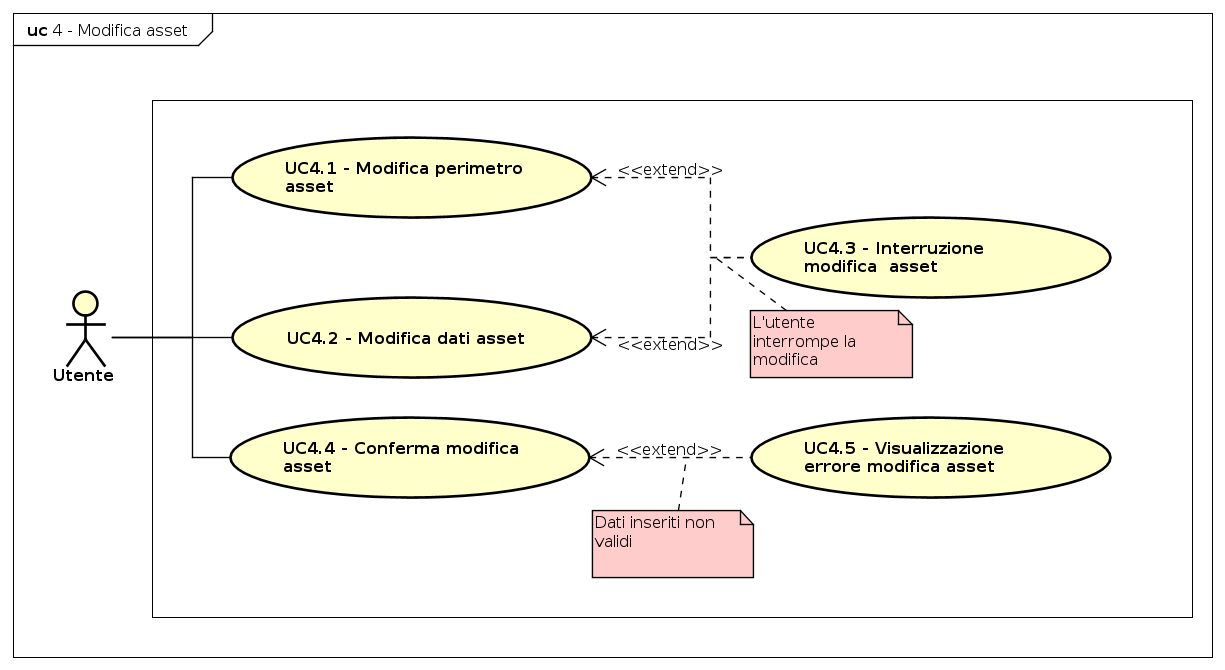
\includegraphics[width=\textwidth]{{img/uc4}.png} 
	\caption{UC4 - Modifica asset}
\end{figure}
\def\arraystretch{1.5}
\rowcolors{2}{D}{P}
\begin{tabularx}{\textwidth}{l|p{0.7\textwidth}}
	\rowcolor{I} \multicolumn{2}{c}{\color{white}\textbf{UC4 - Modifica asset}} \\
	\toprule
	\endhead
	\textbf{Attori} & Utente\\
	\textbf{Descrizione} & l'utente modifica l'asset\\
	\textbf{Pre-condizione} & l'utente ha aperto l'applicazione; almeno un asset è stato aggiunto; l'utente ha selezionato un asset\\
	\textbf{Post-condizione} & l'asset è stato modificato; l'utente visualizza un messaggio che comunica la corretta esecuzione dell'operazione; l'area informativa rimane impostata sull'asset appena modificato; la posizione e il livello di ingrandimento della mappa rimangono invariati\\
	\textbf{Scenario principale} & \vspace{-1.2em}\begin{enumerate}[leftmargin=*,noitemsep,nosep]
		\item \nameref{sssec:UC4.1};
		\item \nameref{sssec:UC4.2};
		\item \nameref{sssec:UC4.3}.
	\end{enumerate}\\
	\textbf{Estensioni} & \vspace{-1.2em}\begin{itemize}[leftmargin=*,noitemsep,nosep]
		\item \nameref{sssec:UC31}: l’utente interrompe volontariamente la modifica dell’asset;
	\end{itemize}\\
	\textbf{Scenari alternativi} & \vspace{-1.2em}\begin{itemize}[leftmargin=*,noitemsep,nosep]
		\item \nameref{sssec:UC4.4}.
	\end{itemize}\\
	%\textbf{Generalizzazioni} &  \\
	\bottomrule
\end{tabularx}
\subsection{UC4.1 - Modifica perimetro asset} 
\label{sssec:UC4.1} 
\begin{figure}[H] 
	\centering 
	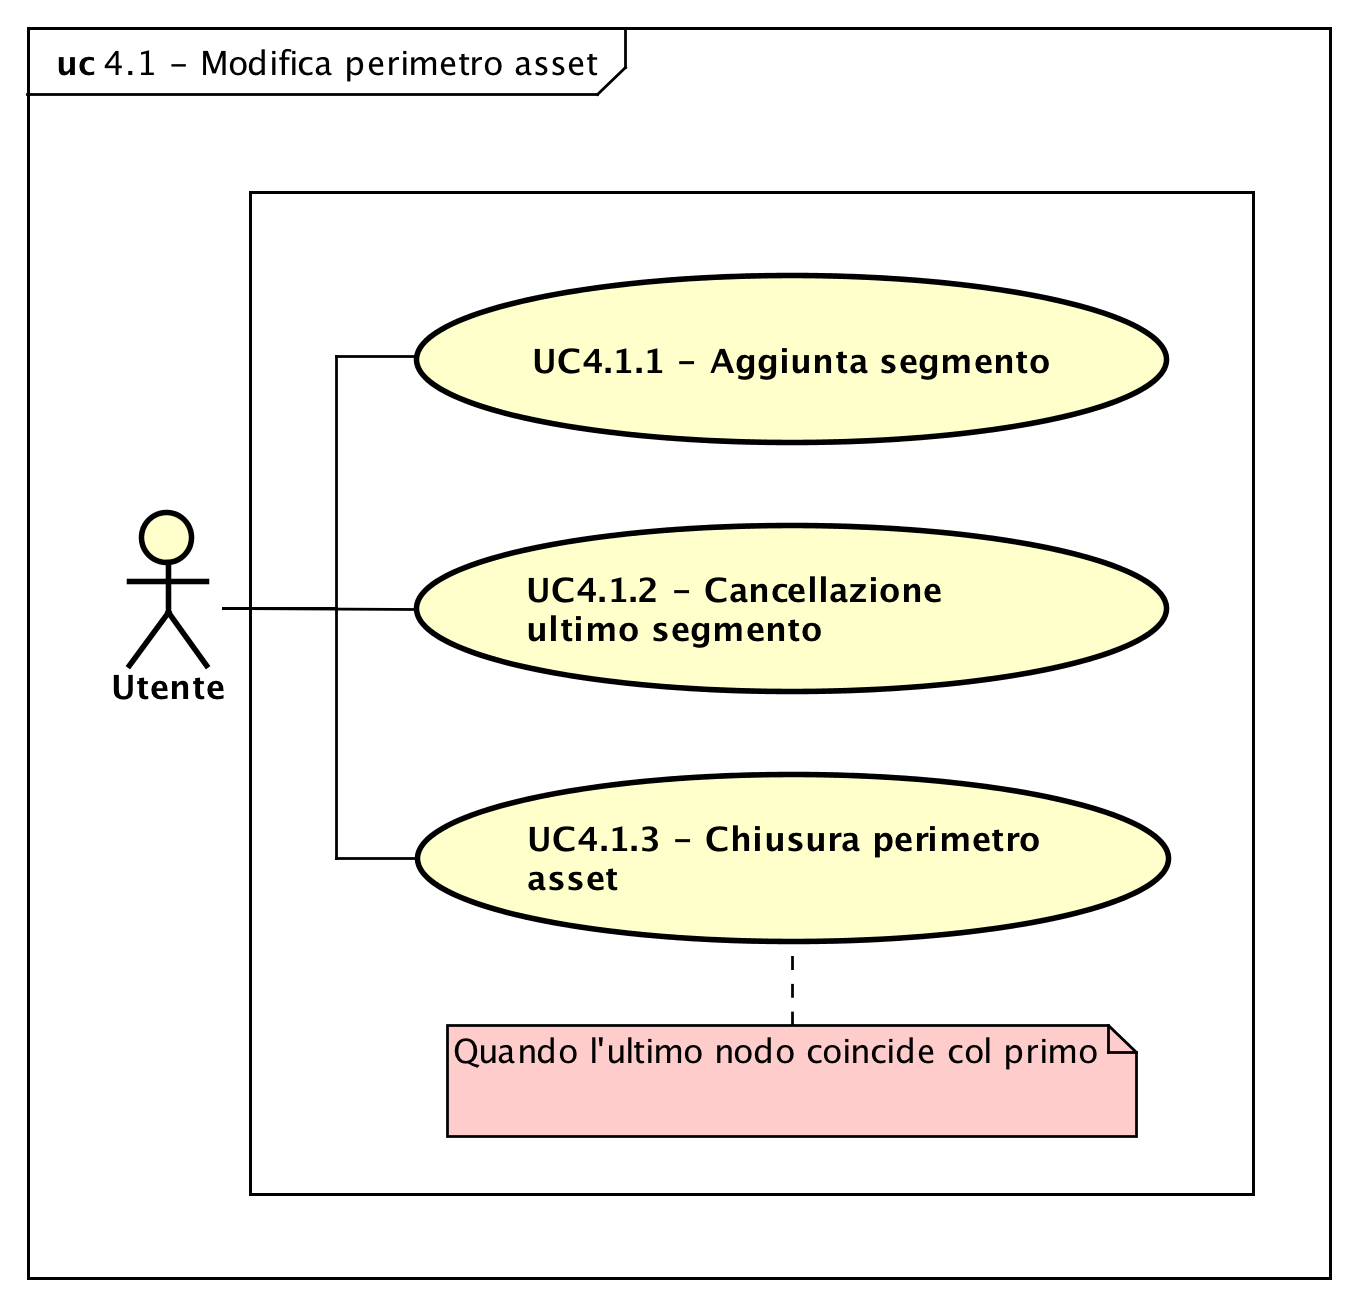
\includegraphics[scale=0.5]{{img/uc4.1}.png} 
	\caption{UC4.1 - Modifica perimetro asset}
\end{figure}
\def\arraystretch{1.5}
\rowcolors{2}{D}{P}
\begin{tabularx}{\textwidth}{l|p{0.7\textwidth}}
	\rowcolor{I} \multicolumn{2}{c}{\color{white}\textbf{UC4.1 - Modifica perimetro asset}} \\
	\toprule
	\endhead
	\textbf{Attori} & Utente\\
	\textbf{Descrizione} & l'utente modifica il perimetro dell'asset\\
	\textbf{Pre-condizione} & il sistema offre la possibilità di modificare il perimetro dell'asset\\
	\textbf{Post-condizione} & il perimetro dell'asset è stato modificato; il nuovo perimetro viene visualizzato sulla mappa; l'utente viene riportato alla schermata di modifica asset\\
	\textbf{Scenario principale} & \vspace{-1.2em}\begin{enumerate}[leftmargin=*,noitemsep,nosep]
		\item \nameref{sssec:UC4.1.1};
		\item \nameref{sssec:UC4.1.2};
		\item \nameref{sssec:UC4.1.3}.
	\end{enumerate}\\
	%\textbf{Generalizzazioni} &  \\
	\bottomrule
\end{tabularx}
\subsection{UC4.1.1 - Aggiunta segmento} 
\label{sssec:UC4.1.1} 
\def\arraystretch{1.5}
\rowcolors{2}{D}{P}
\begin{tabularx}{\textwidth}{l|p{0.7\textwidth}}
	\rowcolor{I} \multicolumn{2}{c}{\color{white}\textbf{UC4.1.1 - Aggiunta segmento}} \\
	\toprule
	\endhead
	\textbf{Attori} & Utente\\
	\textbf{Descrizione} & l'utente aggiunge un segmento al perimetro dell'asset che sta modificando\\
	\textbf{Pre-condizione} & il sistema offre la possibilità di aggiungere un segmento al perimetro dell'asset\\
	\textbf{Post-condizione} & l'utente ha aggiunto un segmento al perimetro dell'asset che sta modificando; il segmento viene visualizzato sulla mappa\\
	\textbf{Scenario principale} & \vspace{-1.2em}\begin{enumerate}[leftmargin=*,noitemsep,nosep]
		\item \nameref{sssec:UC4.1.1}.
	\end{enumerate}\\
	%\textbf{Generalizzazioni} &  \\
	\bottomrule
\end{tabularx}
\subsection{UC4.1.2 - Cancellazione ultimo segmento} 
\label{sssec:UC4.1.2} 
\def\arraystretch{1.5}
\rowcolors{2}{D}{P}
\begin{tabularx}{\textwidth}{l|p{0.7\textwidth}}
	\rowcolor{I} \multicolumn{2}{c}{\color{white}\textbf{UC4.1.2 - Cancellazione ultimo segmento}} \\
	\toprule
	\endhead
	\textbf{Attori} & Utente\\
	\textbf{Descrizione} & l'utente cancella l'ultimo segmento del perimetro dell'asset che sta modificando\\
	\textbf{Pre-condizione} & l'utente sta disegnando il perimetro di un asset; è stato disegnato almeno un segmento\\
	\textbf{Post-condizione} & l'utente ha cancellato l'ultimo segmento del perimetro dell'asset che sta modificando; il segmento non è più visibile sulla mappa\\
	\textbf{Scenario principale} & \vspace{-1.2em}\begin{enumerate}[leftmargin=*,noitemsep,nosep]
		\item \nameref{sssec:UC4.1.2}.
	\end{enumerate}\\
	%\textbf{Generalizzazioni} &  \\
	\bottomrule
\end{tabularx}
\subsection{UC4.1.3 - Chiusura perimetro asset} 
\label{sssec:UC4.1.3} 
\def\arraystretch{1.5}
\rowcolors{2}{D}{P}
\begin{tabularx}{\textwidth}{l|p{0.7\textwidth}}
	\rowcolor{I} \multicolumn{2}{c}{\color{white}\textbf{UC4.1.3 - Chiusura perimetro asset}} \\
	\toprule
	\endhead
	\textbf{Attori} & Utente\\
	\textbf{Descrizione} & l'utente termina di disegnare il perimetro dell'asset che sta modificando, facendo coincidere ultimo e primo nodo\\
	\textbf{Pre-condizione} & il sistema offre la possibilità di disegnare il perimetro dell'asset; l'utente ha disegnato almeno due segmenti\\
	\textbf{Post-condizione} & l'utente ha terminato di disegnare il perimetro di un asset; il perimetro è visualizzato sulla mappa; l'utente può continuare a procedere con la modifica degli altri dati dell'asset sull'area informativa\\
	\textbf{Scenario principale} & \vspace{-1.2em}\begin{enumerate}[leftmargin=*,noitemsep,nosep]
		\item \nameref{sssec:UC4.1.3}.
	\end{enumerate}\\
	%\textbf{Generalizzazioni} &  \\
	\bottomrule
\end{tabularx}
\subsection{UC4.2 - Modifica dati asset} 
\label{sssec:UC4.2} 
\begin{figure}[H] 
	\centering 
	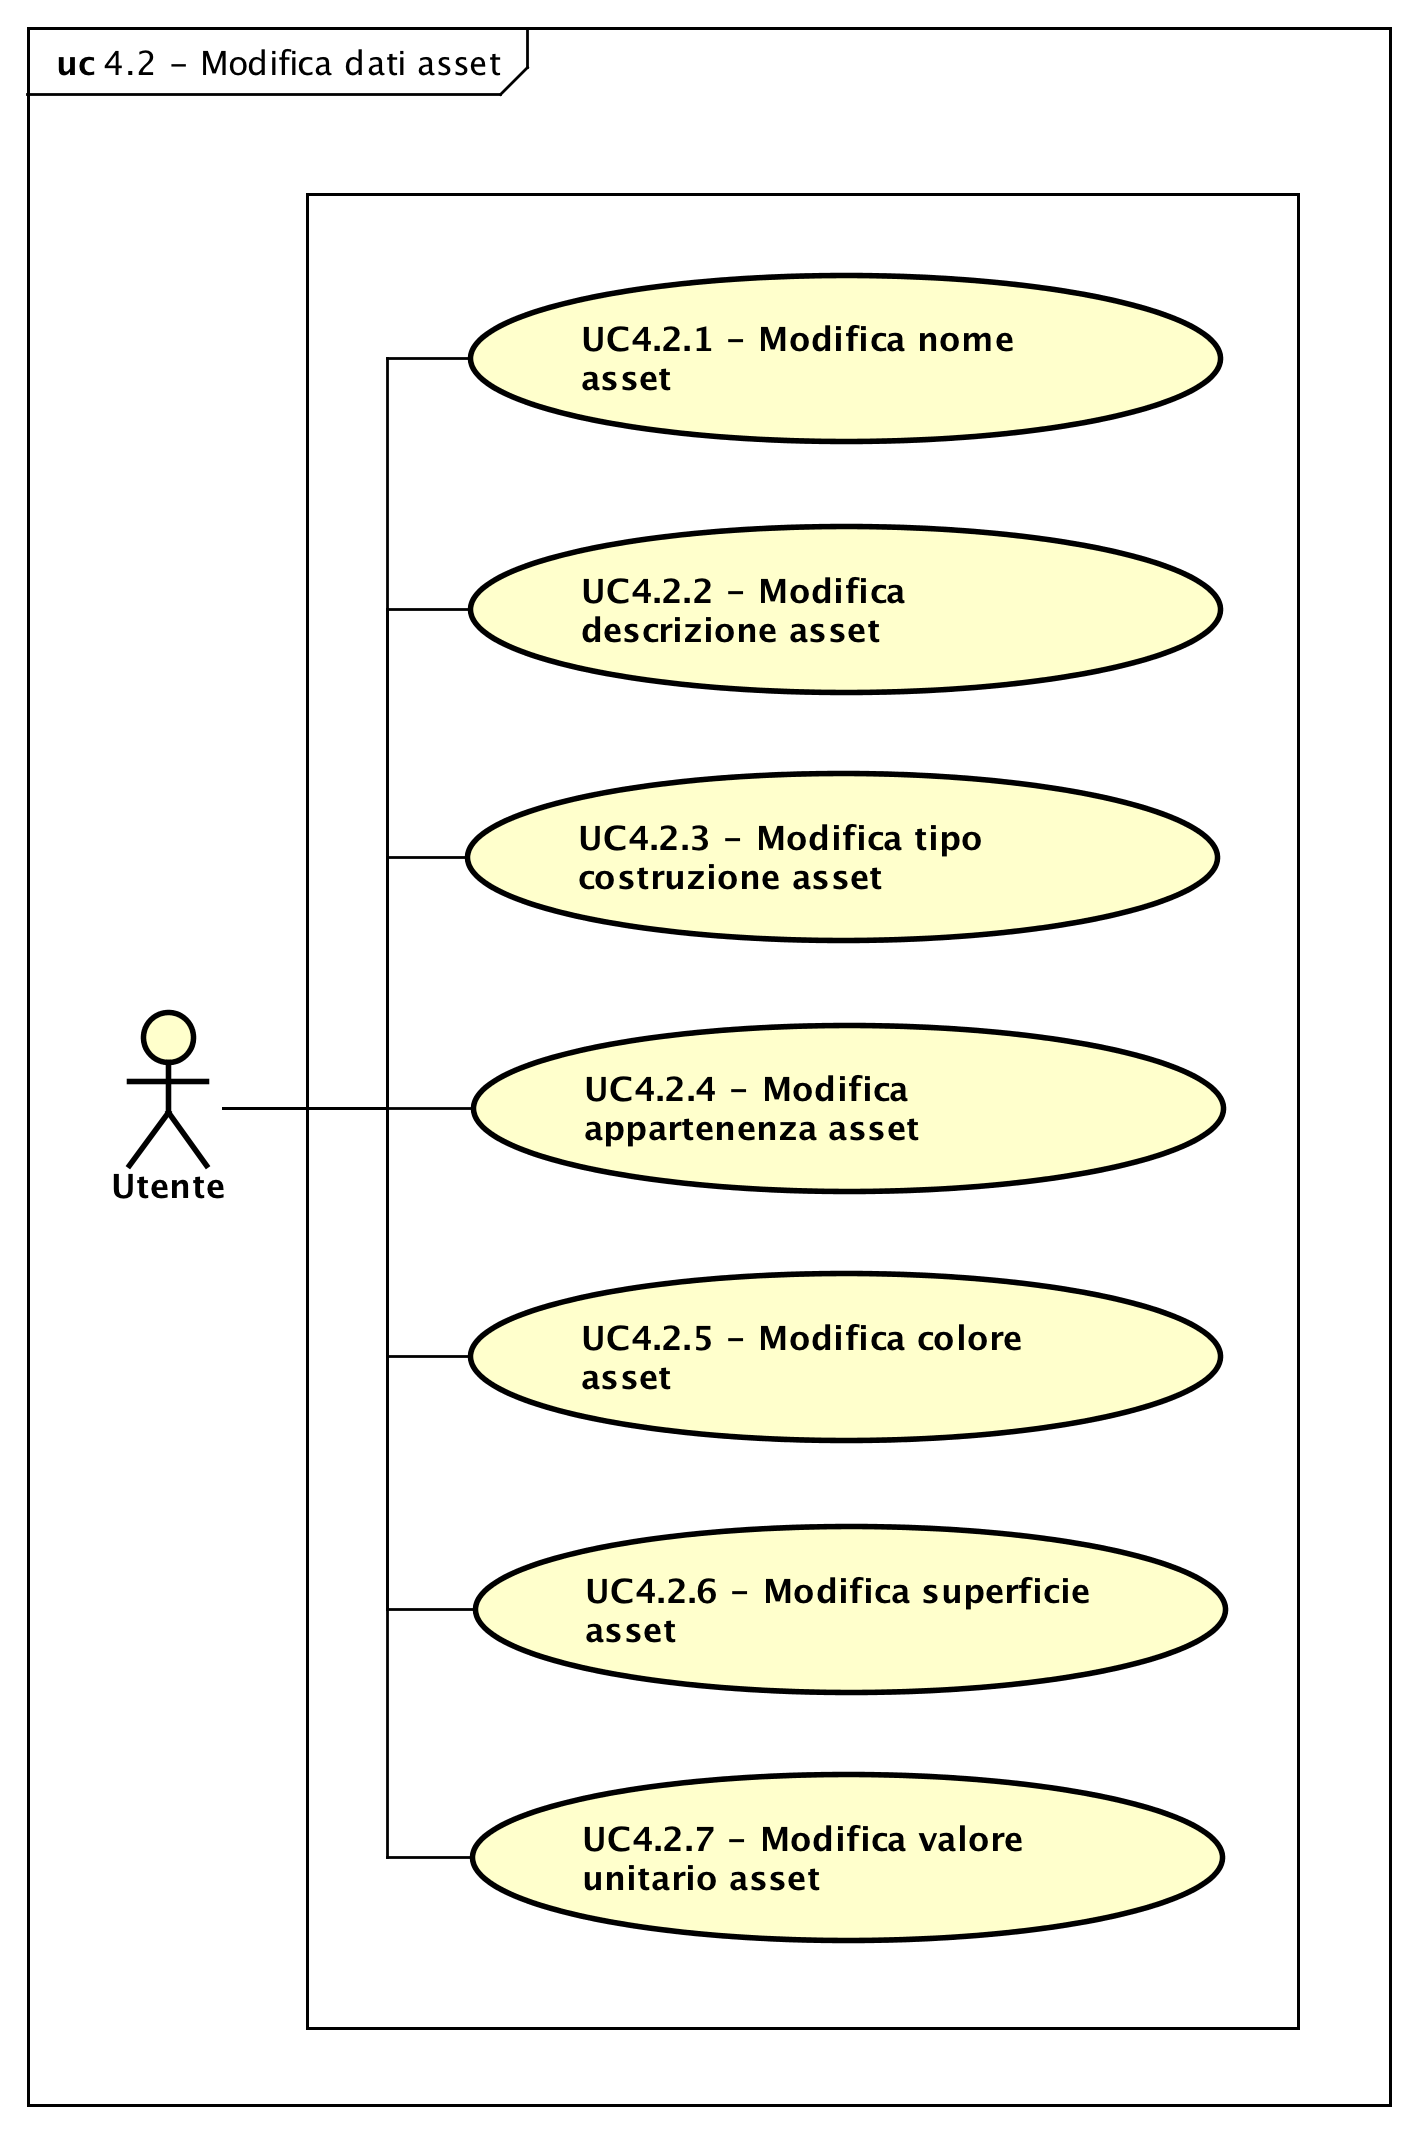
\includegraphics[scale=0.5]{{img/uc4.2}.png} 
	\caption{UC4.2 - Modifica dati asset}
\end{figure}
\def\arraystretch{1.5}
\rowcolors{2}{D}{P}
\begin{tabularx}{\textwidth}{l|p{0.7\textwidth}}
	\rowcolor{I} \multicolumn{2}{c}{\color{white}\textbf{UC4.2 - Modifica dati asset}} \\
	\toprule
	\endhead
	\textbf{Attori} & Utente\\
	\textbf{Descrizione} & l'utente modifica i dati dell'asset\\
	\textbf{Pre-condizione} & il sistema offre la possibilità di modificare i dati dell'asset\\
	\textbf{Post-condizione} & i dati dell'asset sono stati modificati e viene riportato alla schermata di modifica dell'asset\\
	\textbf{Scenario principale} & \vspace{-1.2em}\begin{enumerate}[leftmargin=*,noitemsep,nosep]
		\item \nameref{sssec:UC4.2.1};
		\item \nameref{sssec:UC4.2.2};
		\item \nameref{sssec:UC4.2.3};
		\item \nameref{sssec:UC4.2.4};
		\item \nameref{sssec:UC4.2.5};
		\item \nameref{sssec:UC4.2.6};
		\item \nameref{sssec:UC4.2.7};
		\item \nameref{sssec:UC4.2.8}.
	\end{enumerate}\\
	%\textbf{Generalizzazioni} &  \\
	\bottomrule
\end{tabularx}
\subsection{UC4.2.1 - Modifica nome asset} 
\label{sssec:UC4.2.1} 
\def\arraystretch{1.5}
\rowcolors{2}{D}{P}
\begin{tabularx}{\textwidth}{l|p{0.7\textwidth}}
	\rowcolor{I} \multicolumn{2}{c}{\color{white}\textbf{UC4.2.1 - Modifica nome asset}} \\
	\toprule
	\endhead
	\textbf{Attori} & Utente\\
	\textbf{Descrizione} & l'utente modifica il campo relativo al nome dell'asset\\
	\textbf{Pre-condizione} & il sistema offre la possibilità di modificare il nome dell'asset\\
	\textbf{Post-condizione} & il campo relativo al nome dell'asset è stato modificato; l'utente può visualizzare il nome appena compilato sull'area informativa\\
	\textbf{Scenario principale} & \vspace{-1.2em}\begin{enumerate}[leftmargin=*,noitemsep,nosep]
		\item \nameref{sssec:UC4.2.1}.
	\end{enumerate}\\
	%\textbf{Generalizzazioni} &  \\
	\bottomrule
\end{tabularx}
\subsection{UC4.2.2 - Modifica descrizione asset} 
\label{sssec:UC4.2.2} 
\def\arraystretch{1.5}
\rowcolors{2}{D}{P}
\begin{tabularx}{\textwidth}{l|p{0.7\textwidth}}
	\rowcolor{I} \multicolumn{2}{c}{\color{white}\textbf{UC4.2.2 - Modifica descrizione asset}} \\
	\toprule
	\endhead
	\textbf{Attori} & Utente\\
	\textbf{Descrizione} & l'utente modifica il campo relativo alla descrizione dell'asset\\
	\textbf{Pre-condizione} & il sistema offre la possibilità di modificare la descrizione dell'asset\\
	\textbf{Post-condizione} & il campo relativo alla descrizione dell'asset è stato modificato; l'utente può visualizzare la descrizione appena compilata sull'area informativa\\
	\textbf{Scenario principale} & \vspace{-1.2em}\begin{enumerate}[leftmargin=*,noitemsep,nosep]
		\item \nameref{sssec:UC4.2.2}.
	\end{enumerate}\\
	%\textbf{Generalizzazioni} &  \\
	\bottomrule
\end{tabularx}
\subsection{UC4.2.3 - Modifica tipo costruzione asset} 
\label{sssec:UC4.2.3} 
\def\arraystretch{1.5}
\rowcolors{2}{D}{P}
\begin{tabularx}{\textwidth}{l|p{0.7\textwidth}}
	\rowcolor{I} \multicolumn{2}{c}{\color{white}\textbf{UC4.2.3 - Modifica tipo costruzione asset}} \\
	\toprule
	\endhead
	\textbf{Attori} & Utente\\
	\textbf{Descrizione} & l'utente modifica la scelta relativa al tipo di costruzione dell'asset\\
	\textbf{Pre-condizione} & il sistema offre la possibilità di modificare il tipo di costruzione dell'asset\\
	\textbf{Post-condizione} & la scelta relativa al tipo di costruzione dell'asset è stata modificata; l'utente può visualizzare la scelta appena effettuata sull'area informativa\\
	\textbf{Scenario principale} & \vspace{-1.2em}\begin{enumerate}[leftmargin=*,noitemsep,nosep]
		\item \nameref{sssec:UC4.2.3}.
	\end{enumerate}\\
	%\textbf{Generalizzazioni} &  \\
	\bottomrule
\end{tabularx}
\subsection{UC4.2.4 - Modifica appartenenza asset} 
\label{sssec:UC4.2.4} 
\def\arraystretch{1.5}
\rowcolors{2}{D}{P}
\begin{tabularx}{\textwidth}{l|p{0.7\textwidth}}
	\rowcolor{I} \multicolumn{2}{c}{\color{white}\textbf{UC4.2.4 - Modifica appartenenza asset}} \\
	\toprule
	\endhead
	\textbf{Attori} & Utente\\
	\textbf{Descrizione} & l'utente modifica la scelta relativa al proprietario dell'asset\\
	\textbf{Pre-condizione} & il sistema offre la possibilità di modificare l'appartenenza dell'asset\\
	\textbf{Post-condizione} & la scelta relativa la proprietario dell'asset è stata modificata; l'utente può visualizzare la scelta appena effettuata sull'area informativa\\
	\textbf{Scenario principale} & \vspace{-1.2em}\begin{enumerate}[leftmargin=*,noitemsep,nosep]
		\item \nameref{sssec:UC4.2.4}.
	\end{enumerate}\\
	%\textbf{Generalizzazioni} &  \\
	\bottomrule
\end{tabularx}
\subsection{UC4.2.5 - Modifica colore asset} 
\label{sssec:UC4.2.5} 
\def\arraystretch{1.5}
\rowcolors{2}{D}{P}
\begin{tabularx}{\textwidth}{l|p{0.7\textwidth}}
	\rowcolor{I} \multicolumn{2}{c}{\color{white}\textbf{UC4.2.5 - Modifica colore asset}} \\
	\toprule
	\endhead
	\textbf{Attori} & Utente\\
	\textbf{Descrizione} & l'utente modifica la scelta relativa al colore dell'asset\\
	\textbf{Pre-condizione} & il sistema offre la possibilità di modificare il colore dell'asset\\
	\textbf{Post-condizione} & la scelta relativa al colore dell'asset è stata modificata; l'utente può visualizzare il colore appena scelto sull'area informativa\\
	\textbf{Scenario principale} & \vspace{-1.2em}\begin{enumerate}[leftmargin=*,noitemsep,nosep]
		\item \nameref{sssec:UC4.2.5}.
	\end{enumerate}\\
	%\textbf{Generalizzazioni} &  \\
	\bottomrule
\end{tabularx}
\subsection{UC4.2.6 - Modifica superficie asset} 
\label{sssec:UC4.2.6} 
\def\arraystretch{1.5}
\rowcolors{2}{D}{P}
\begin{tabularx}{\textwidth}{l|p{0.7\textwidth}}
	\rowcolor{I} \multicolumn{2}{c}{\color{white}\textbf{UC4.2.6 - Modifica superficie asset}} \\
	\toprule
	\endhead
	\textbf{Attori} & Utente\\
	\textbf{Descrizione} & l'utente modifica il campo relativo alla superficie dell'asset\\
	\textbf{Pre-condizione} & il sistema offre la possibilità di modificare la superficie dell'asset\\
	\textbf{Post-condizione} & il campo relativo alla superficie dell'asset è stato modificato; l'utente può visualizzare la superficie appena compilata sull'area informativa\\
	\textbf{Scenario principale} & \vspace{-1.2em}\begin{enumerate}[leftmargin=*,noitemsep,nosep]
		\item \nameref{sssec:UC4.2.6}.
	\end{enumerate}\\
	%\textbf{Generalizzazioni} &  \\
	\bottomrule
\end{tabularx}
\subsection{UC4.2.7 - Modifica valore unitario asset} 
\label{sssec:UC4.2.7} 
\def\arraystretch{1.5}
\rowcolors{2}{D}{P}
\begin{tabularx}{\textwidth}{l|p{0.7\textwidth}}
	\rowcolor{I} \multicolumn{2}{c}{\color{white}\textbf{UC4.2.7 - Modifica valore unitario asset}} \\
	\toprule
	\endhead
	\textbf{Attori} & Utente\\
	\textbf{Descrizione} & l'utente modifica il campo relativo al valore unitario dell'asset\\
	\textbf{Pre-condizione} & il sistema offre la possibilità di modificare il valore unitario dell'asset\\
	\textbf{Post-condizione} & il campo relativo al valore unitario dell'asset è stato modificato; l'utente può visualizzare il valore unitario appena compilato sull'area informativa\\
	\textbf{Scenario principale} & \vspace{-1.2em}\begin{enumerate}[leftmargin=*,noitemsep,nosep]
		\item \nameref{sssec:UC4.2.7}.
	\end{enumerate}\\
	%\textbf{Generalizzazioni} &  \\
	\bottomrule
\end{tabularx}
\subsection{UC4.3 - Conferma modifica asset} 
\label{sssec:UC4.3} 
\def\arraystretch{1.5}
\rowcolors{2}{D}{P}
\begin{tabularx}{\textwidth}{l|p{0.7\textwidth}}
	\rowcolor{I} \multicolumn{2}{c}{\color{white}\textbf{UC4.3 - Conferma modifica asset}} \\
	\toprule
	\endhead
	\textbf{Attori} & Utente\\
	\textbf{Descrizione} & l'utente conferma la modifica dell'asset\\
	\textbf{Pre-condizione} & il sistema offre la possibilità di confermare la modifica dell'asset\\
	\textbf{Post-condizione} & l'asset è stato modificato; l'utente visualizza un messaggio che comunica la corretta esecuzione dell'operazione; l'area informativa rimane impostata sull'asset appena modificato; la posizione e il livello di ingrandimento della mappa rimangono invariati\\
	\textbf{Scenario principale} & \vspace{-1.2em}\begin{enumerate}[leftmargin=*,noitemsep,nosep]
		\item \nameref{sssec:UC4.3}.
	\end{enumerate}\\
	\textbf{Estensioni} & \vspace{-1.2em}\begin{itemize}[leftmargin=*,noitemsep,nosep]
		\item \nameref{sssec:UC4.4}: dati inseriti non validi:
		\begin{itemize}
			\item nome vuoto; più lungo di 50 caratteri;
			inizia e/o finisce con uno spazio; contiene caratteri speciali;
			\item descrizione vuota; più lunga di 5000
			caratteri; inizia e/o finisce con uno spazio; contiene caratteri
			speciali diversi dall'apostrofo;
			\item tipo di costruzione non scelto;
			\item appartenenza non scelta;
			\item colore non scelto;
			\item superficie (in mq) vuota; più lunga di
			5 cifre per la parte intera; più di 2 per la parte decimale;
			\item valore unitario (monetario) vuoto; più
			lungo di 20 cifre per la parte intera; più di 2 per la parte
			decimale;
			\item valuta non scelta
		\end{itemize}
	\end{itemize}\\
	%\textbf{Generalizzazioni} &  \\
	\bottomrule
\end{tabularx}
\subsection{UC4.4 - Visualizzazione errore modifica asset} 
\label{sssec:UC4.4} 
\def\arraystretch{1.5}
\rowcolors{2}{D}{P}
\begin{tabularx}{\textwidth}{l|p{0.7\textwidth}}
	\rowcolor{I} \multicolumn{2}{c}{\color{white}\textbf{UC4.4 - Visualizzazione errore modifica asset}} \\
	\toprule
	\endhead
	\textbf{Attori} & Utente\\
	\textbf{Descrizione} & l'utente visualizza un errore relativo alla modifica dell'asset\\
	\textbf{Pre-condizione} & l'utente ha confermato la modifica dei dati dell'asset\\
	\textbf{Post-condizione} & l'asset non è stato modificato; l'utente visualizza un errore relativo ai dati dell'asset compilati in modo errato; l'utente viene riportato alla schermata di modifica asset\\
	\textbf{Scenario principale} & \vspace{-1.2em}\begin{enumerate}[leftmargin=*,noitemsep,nosep]
		\item \nameref{sssec:UC4.4}.
	\end{enumerate}\\
	%\textbf{Generalizzazioni} &  \\
	\bottomrule
\end{tabularx}

\subsection{UC5 - Eliminazione asset} 
\label{sssec:UC5} 
\begin{figure}[H] 
	\centering 
	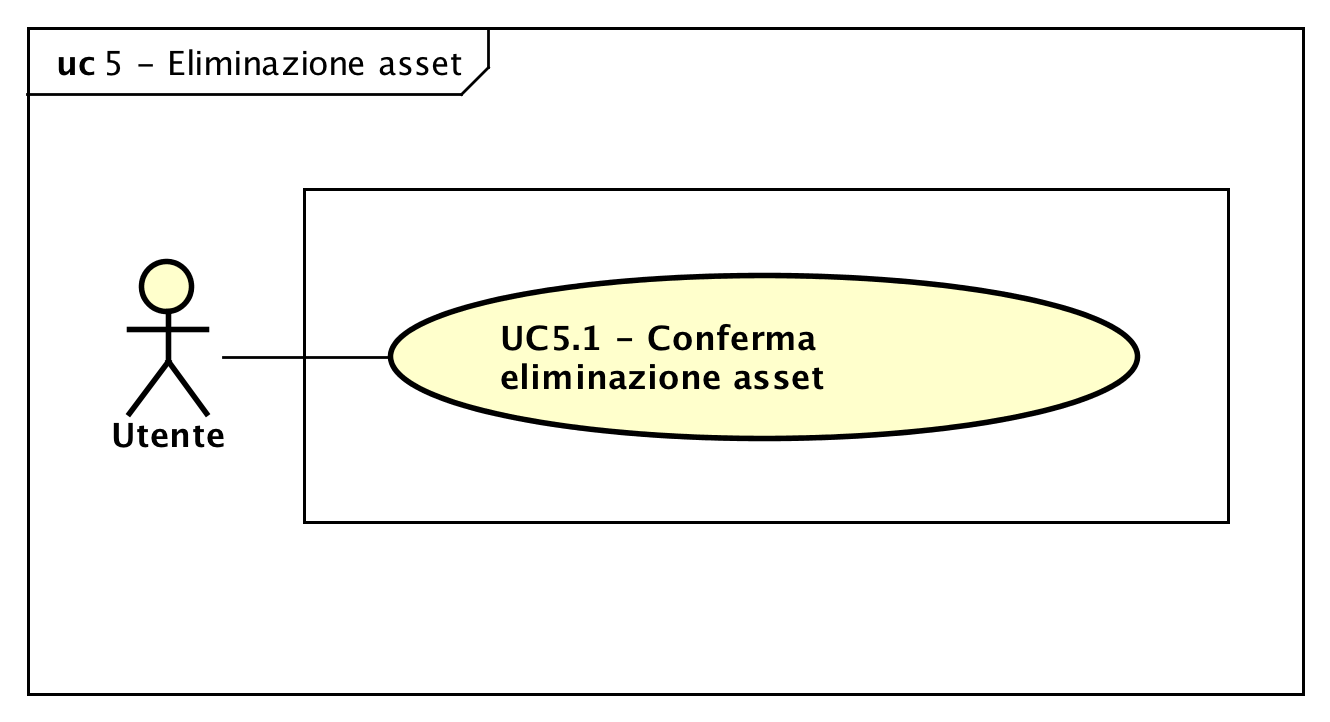
\includegraphics[scale=0.5]{{img/uc5}.png} 
	\caption{UC5 - Eliminazione asset}
\end{figure}
\def\arraystretch{1.5}
\rowcolors{2}{D}{P}
\begin{tabularx}{\textwidth}{l|p{0.7\textwidth}}
	\rowcolor{I} \multicolumn{2}{c}{\color{white}\textbf{UC5 - Eliminazione asset}} \\
	\toprule
	\endhead
	\textbf{Attori} & Utente\\
	\textbf{Descrizione} & l'utente elimina un asset\\
	\textbf{Pre-condizione} & l'utente ha aperto l'applicazione; è stato inserito almeno un asset; l'utente ha selezionato un asset\\
	\textbf{Post-condizione} & l'asset è stato eliminato e non è più visualizzabile sulla mappa; vengono eliminati tutti i nodi contenuti nell'asset; l'utente visualizza un messaggio che comunica la corretta esecuzione dell'operazione; l'area informativa viene impostata sulla visualizzazione di default;  la posizione e il livello di ingrandimento della mappa rimangono invariati\\
	\textbf{Scenario principale} & \vspace{-1.2em}\begin{enumerate}[leftmargin=*,noitemsep,nosep]
		\item \nameref{sssec:UC5.1}.
	\end{enumerate}\\
	\textbf{Estensioni} & \vspace{-1.2em}\begin{itemize}[leftmargin=*,noitemsep,nosep]
		\item \nameref{sssec:UC32}: l'utente interrompe volontariamente l'eliminazione dell'asset.
	\end{itemize}\\
	%\textbf{Generalizzazioni} &  \\
	\bottomrule
\end{tabularx}
\subsection{UC5.1 - Conferma eliminazione asset} 
\label{sssec:UC5.1} 
\def\arraystretch{1.5}
\rowcolors{2}{D}{P}
\begin{tabularx}{\textwidth}{l|p{0.7\textwidth}}
	\rowcolor{I} \multicolumn{2}{c}{\color{white}\textbf{UC5.1 - Conferma eliminazione asset}} \\
	\toprule
	\endhead
	\textbf{Attori} & Utente\\
	\textbf{Descrizione} & l'utente conferma l'eliminazione dell'asset\\
	\textbf{Pre-condizione} & il sistema offre la possibilità di confermare l'eliminazione dell'asset\\
	\textbf{Post-condizione} & l'asset è stato eliminato e non è più visibile sulla mappa; l'utente visualizza un messaggio che comunica la corretta esecuzione dell'operazione;  l'area informativa viene impostata sulla visualizzazione di default; la posizione e il livello di ingrandimento della mappa rimangono invariati\\
	\textbf{Scenario principale} & \vspace{-1.2em}\begin{enumerate}[leftmargin=*,noitemsep,nosep]
		\item \nameref{sssec:UC5.1}.
	\end{enumerate}\\
	%\textbf{Generalizzazioni} &  \\
	\bottomrule
\end{tabularx}
\subsection{UC6 - Aggiunta nodo} 
\label{sssec:UC6} 
\begin{figure}[H] 
	\centering 
	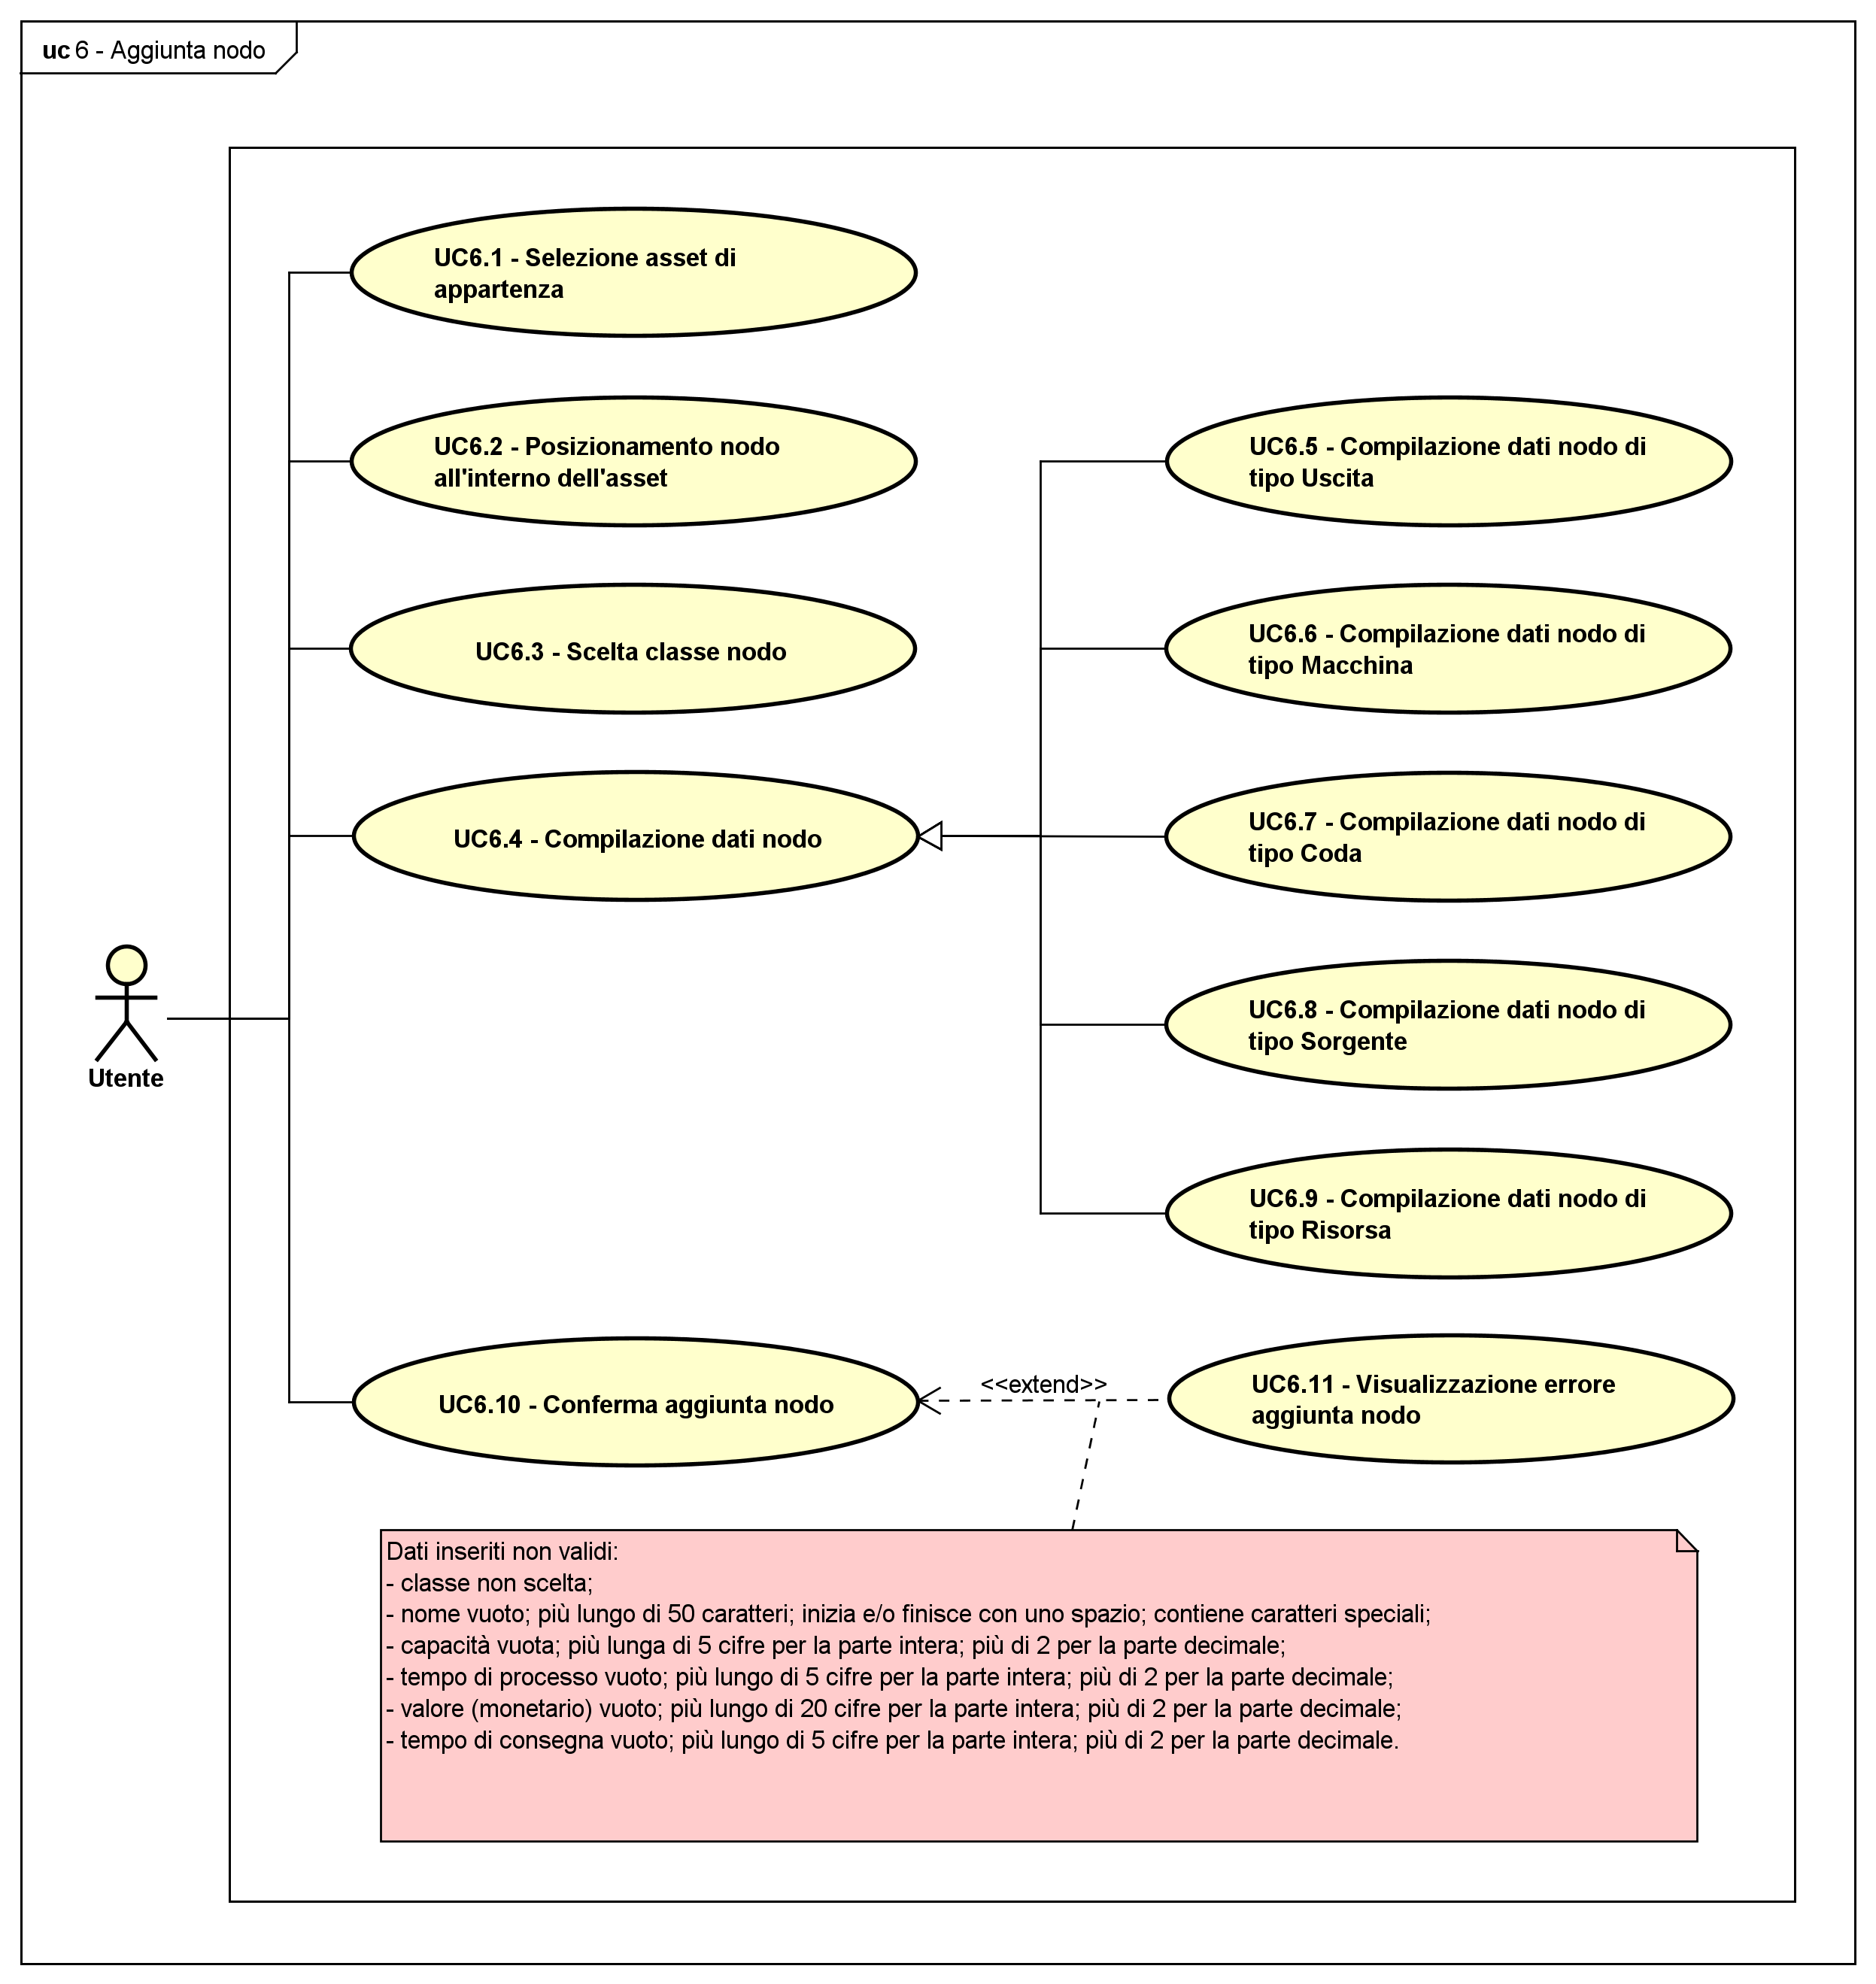
\includegraphics[width=\textwidth]{{img/uc6}.png} 
	\caption{UC6 - Aggiunta nodo}
\end{figure}
\def\arraystretch{1.5}
\rowcolors{2}{D}{P}
\begin{tabularx}{\textwidth}{l|p{0.7\textwidth}}
	\rowcolor{I} \multicolumn{2}{c}{\color{white}\textbf{UC6 - Aggiunta nodo}} \\
	\toprule
	\endhead
	\textbf{Attori} & Utente\\
	\textbf{Descrizione} & l'utente aggiunge un nodo\\
	\textbf{Pre-condizione} & l'utente ha aperto l'applicazione; è stato inserito almeno un asset\\
	\textbf{Post-condizione} & un nuovo nodo è stato aggiunto ed è visualizzabile sulla mappa; l'utente visualizza un messaggio che comunica la corretta esecuzione dell'operazione; l'area informativa rimane impostata sul nodo appena inserito; la posizione e il livello di ingrandimento della mappa rimangono invariati\\
	\textbf{Scenario principale} & \vspace{-1.2em}\begin{enumerate}[leftmargin=*,noitemsep,nosep]
		\item \nameref{sssec:UC6.1};
		\item \nameref{sssec:UC6.2};
		\item \nameref{sssec:UC6.3};
		\item \nameref{sssec:UC6.4};
		\item \nameref{sssec:UC6.5} oppure
		\item \nameref{sssec:UC6.6} oppure
		\item \nameref{sssec:UC6.7} oppure
		\item \nameref{sssec:UC6.8} oppure
		\item \nameref{sssec:UC6.9} oppure
		\item \nameref{sssec:UC6.10}.
	\end{enumerate}\\
	\textbf{Estensioni} & \vspace{-1.2em}\begin{itemize}[leftmargin=*,noitemsep,nosep]
		\item \nameref{sssec:UC33}: l'utente interrompe volontariamente l'aggiunta del nodo.
	\end{itemize}\\
	\textbf{Scenari alternativi} & \vspace{-1.2em}\begin{itemize}[leftmargin=*,noitemsep,nosep]
		\item \nameref{sssec:UC6.11}.
	\end{itemize}\\
	%\textbf{Generalizzazioni} &  \\
	\bottomrule
\end{tabularx}
\subsection{UC6.1 - Selezione asset di appartenenza} 
\label{sssec:UC6.1} 
\def\arraystretch{1.5}
\rowcolors{2}{D}{P}
\begin{tabularx}{\textwidth}{l|p{0.7\textwidth}}
	\rowcolor{I} \multicolumn{2}{c}{\color{white}\textbf{UC6.1 - Selezione asset di appartenenza}} \\
	\toprule
	\endhead
	\textbf{Attori} & Utente\\
	\textbf{Descrizione} & l'utente seleziona un asset\\
	\textbf{Pre-condizione} & il sistema offre la possibilità di selezionare l'asset di appartenenza\\
	\textbf{Post-condizione} & l'asset di appartenenza è stato selezionato; l'utente può continuare a posizionare il nodo e compilare le altre informazioni\\
	\textbf{Scenario principale} & \vspace{-1.2em}\begin{enumerate}[leftmargin=*,noitemsep,nosep]
		\item \nameref{sssec:UC6.1}.
	\end{enumerate}\\
	%\textbf{Generalizzazioni} &  \\
	\bottomrule
\end{tabularx}

\subsection{UC6.2 - Posizionamento nodo all'interno dell'asset} 
\label{sssec:UC6.2} 
\def\arraystretch{1.5}
\rowcolors{2}{D}{P}
\begin{tabularx}{\textwidth}{l|p{0.7\textwidth}}
	\rowcolor{I} \multicolumn{2}{c}{\color{white}\textbf{UC6.2 - Posizionamento nodo all'interno dell'asset}} \\
	\toprule
	\endhead
	\textbf{Attori} & Utente\\
	\textbf{Descrizione} & il sistema offre la possibilità di posizionare il nodo all'interno dell'asset\\
	\textbf{Pre-condizione} & l'utente ha selezionato l'asset di appartenenza\\
	\textbf{Post-condizione} & il nodo è stato posizionato all'interno dell'asset ed è visibile sulla mappa\\
	\textbf{Scenario principale} & \vspace{-1.2em}\begin{enumerate}[leftmargin=*,noitemsep,nosep]
		\item \nameref{sssec:UC6.2}.
	\end{enumerate}\\
	%\textbf{Generalizzazioni} &  \\
	\bottomrule
\end{tabularx}
\subsection{UC6.3 - Scelta classe nodo} 
\label{sssec:UC6.3} 
\def\arraystretch{1.5}
\rowcolors{2}{D}{P}
\begin{tabularx}{\textwidth}{l|p{0.7\textwidth}}
	\rowcolor{I} \multicolumn{2}{c}{\color{white}\textbf{UC6.3 - Scelta classe nodo}} \\
	\toprule
	\endhead
	\textbf{Attori} & Utente\\
	\textbf{Descrizione} & il sistema offre la possibilità di scegliere la classe del nodo\\
	\textbf{Pre-condizione} & l'utente ha posizionato il nodo all'interno dell'asset\\
	\textbf{Post-condizione} & la classe del nodo è stata scelta; la forma del nodo sulla mappa viene cambiata in base alla classe scelta\\
	\textbf{Scenario principale} & \vspace{-1.2em}\begin{enumerate}[leftmargin=*,noitemsep,nosep]
		\item \nameref{sssec:UC6.3}.
	\end{enumerate}\\
	%\textbf{Generalizzazioni} &  \\
	\bottomrule
\end{tabularx}
\subsection{UC6.4 - Compilazione dati nodo} 
\label{sssec:UC6.4} 
\begin{figure}[H] 
	\centering 
	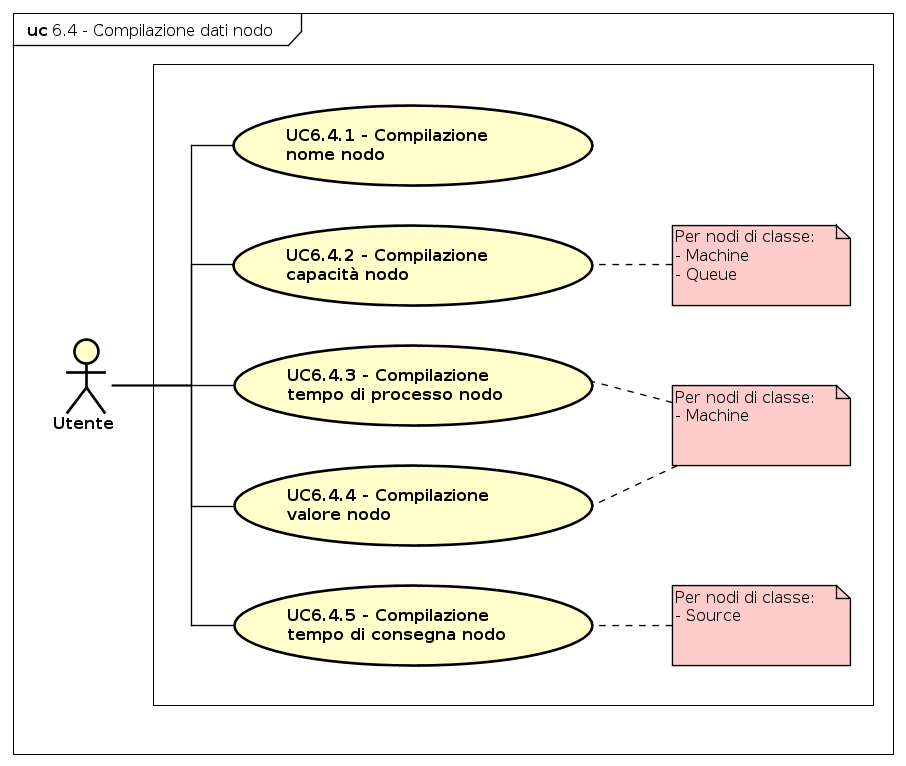
\includegraphics[scale=0.5]{{img/uc6.4}.png} 
	\caption{UC6.4 - Compilazione dati nodo}
\end{figure}
\def\arraystretch{1.5}
\rowcolors{2}{D}{P}
\begin{tabularx}{\textwidth}{l|p{0.7\textwidth}}
	\rowcolor{I} \multicolumn{2}{c}{\color{white}\textbf{UC6.4 - Compilazione dati nodo}} \\
	\toprule
	\endhead
	\textbf{Attori} & Utente\\
	\textbf{Descrizione} & il sistema offre la possibilità di compilare i dati del nodo\\
	\textbf{Pre-condizione} & l'utente ha posizionato il nodo;\\
	\textbf{Post-condizione} & i dati del nodo sono stati compilati; l'utente visualizza i dati appena compilati nell'area informativa\\
	\textbf{Scenario principale} & \vspace{-1.2em}\begin{enumerate}[leftmargin=*,noitemsep,nosep]
		\item \nameref{sssec:UC6.4.1}.
	\end{enumerate}\\
	\textbf{Generalizzazioni} & \vspace{-1.2em}
	\begin{itemize}[leftmargin=*,noitemsep,nosep]
		\item \nameref{sssec:UC6.5};
		\item \nameref{sssec:UC6.6};
		\item \nameref{sssec:UC6.7};
		\item \nameref{sssec:UC6.8};
		\item \nameref{sssec:UC6.9}.
	\end{itemize} \\
	\bottomrule
\end{tabularx}
\subsection{UC6.4.1 - Compilazione nome nodo} 
\label{sssec:UC6.4.1} 
\def\arraystretch{1.5}
\rowcolors{2}{D}{P}
\begin{tabularx}{\textwidth}{l|p{0.7\textwidth}}
	\rowcolor{I} \multicolumn{2}{c}{\color{white}\textbf{UC6.4.1 - Compilazione nome nodo}} \\
	\toprule
	\endhead
	\textbf{Attori} & Utente\\
	\textbf{Descrizione} & l'utente compila il nome del nodo\\
	\textbf{Pre-condizione} & il sistema offre la possibilità di compilare il nome del nodo\\
	\textbf{Post-condizione} & l'utente ha compilato il nome del nodo e visualizza il nome appena compilato nell'area informativa\\
	\textbf{Scenario principale} & \vspace{-1.2em}\begin{enumerate}[leftmargin=*,noitemsep,nosep]
		\item \nameref{sssec:UC6.4.1}.
	\end{enumerate}\\
	%\textbf{Generalizzazioni} &  \\
	\bottomrule
\end{tabularx}
\subsection{UC6.5 - Compilazione dati nodo di tipo Uscita} 
\label{sssec:UC6.5} 
\def\arraystretch{1.5}
\rowcolors{2}{D}{P}
\begin{tabularx}{\textwidth}{l|p{0.7\textwidth}}
	\rowcolor{I} \multicolumn{2}{c}{\color{white}\textbf{UC6.5 - Compilazione dati nodo di tipo Uscita}} \\
	\toprule
	\endhead
	\textbf{Attori} & Utente\\
	\textbf{Descrizione} & l'utente compila i dati del nodo di tipo Uscita\\
	\textbf{Pre-condizione} & l'utente ha posizionato il nodo; l'utente ha scelto come tipologia di nodo Uscita\\
	\textbf{Post-condizione} & i dati del nodo di tipo Uscita sono stati compilati; l'utente visualizza i dati appena compilati nell'area informativa\\
	\textbf{Scenario principale} & \vspace{-1.2em}\begin{enumerate}[leftmargin=*,noitemsep,nosep]
		\item \nameref{sssec:UC6.5}.
	\end{enumerate}\\
	%\textbf{Generalizzazioni} &  \\
	\bottomrule
\end{tabularx}
\subsection{UC6.6 - Compilazione dati nodo di tipo Macchina} 
\label{sssec:UC6.6} 
\begin{figure}[H] 
	\centering 
	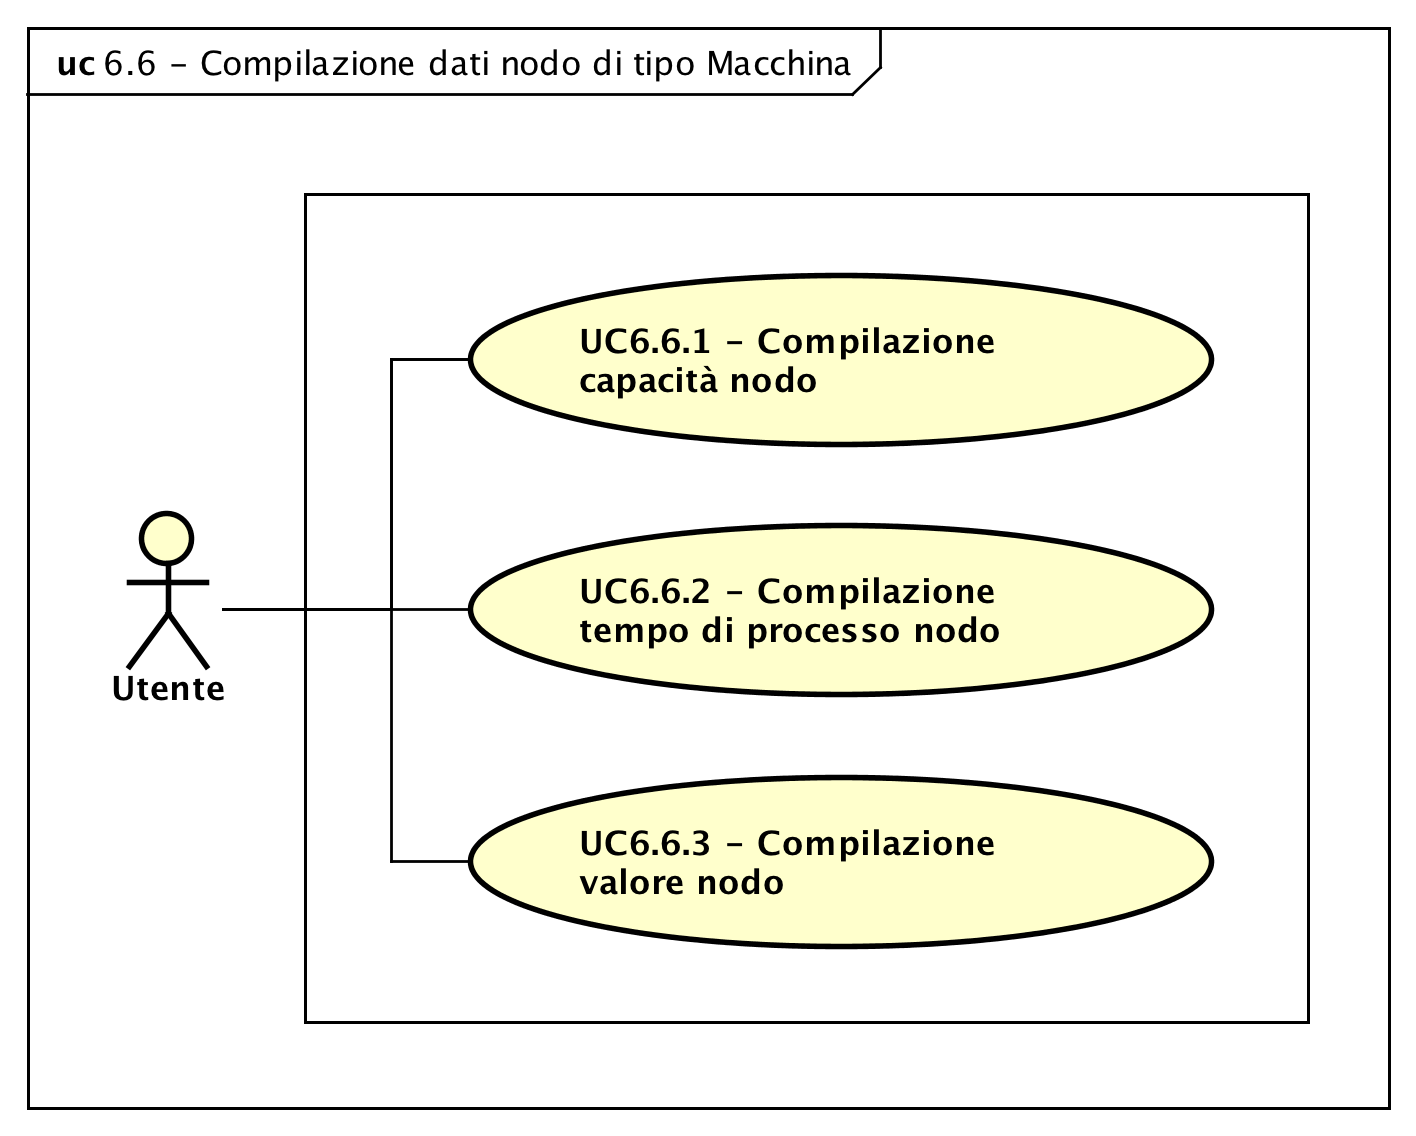
\includegraphics[scale=0.5]{{img/uc6.6}.png} 
	\caption{UC6.6 - Compilazione dati nodo di tipo Macchina}
\end{figure}
\def\arraystretch{1.5}
\rowcolors{2}{D}{P}
\begin{tabularx}{\textwidth}{l|p{0.7\textwidth}}
	\rowcolor{I} \multicolumn{2}{c}{\color{white}\textbf{UC6.6 - Compilazione dati nodo di tipo Macchina}} \\
	\toprule
	\endhead
	\textbf{Attori} & Utente\\
	\textbf{Descrizione} & l'utente compila i dati del nodo di tipo Macchina\\
	\textbf{Pre-condizione} & l'utente ha posizionato il nodo; l'utente ha scelto come tipologia di nodo Macchina\\
	\textbf{Post-condizione} & i dati del nodo di tipo Macchina sono stati compilati; l'utente visualizza i dati appena compilati nell'area informativa\\
	\textbf{Scenario principale} & \vspace{-1.2em}\begin{enumerate}[leftmargin=*,noitemsep,nosep]
		\item \nameref{sssec:UC6.6.1};
		\item \nameref{sssec:UC6.6.2};
		\item \nameref{sssec:UC6.6.3}.
	\end{enumerate}\\
	%\textbf{Generalizzazioni} &  \\
	\bottomrule
\end{tabularx}
\subsection{UC6.6.1 - Compilazione capacità nodo} 
\label{sssec:UC6.6.1} 
\def\arraystretch{1.5}
\rowcolors{2}{D}{P}
\begin{tabularx}{\textwidth}{l|p{0.7\textwidth}}
	\rowcolor{I} \multicolumn{2}{c}{\color{white}\textbf{UC6.6.1 - Compilazione capacità nodo}} \\
	\toprule
	\endhead
	\textbf{Attori} & Utente\\
	\textbf{Descrizione} & l'utente compila la capacità del nodo\\
	\textbf{Pre-condizione} & il sistema offre la possibilità di compilare il nome del nodo; l'utente ha scelto come tipologia di nodo Macchina o Coda\\
	\textbf{Post-condizione} & l'utente ha compilato la capacità del nodo e visualizza la capacità appena compilata nell'area informativa\\
	\textbf{Scenario principale} & \vspace{-1.2em}\begin{enumerate}[leftmargin=*,noitemsep,nosep]
		\item \nameref{sssec:UC6.6.1}.
	\end{enumerate}\\
	%\textbf{Generalizzazioni} &  \\
	\bottomrule
\end{tabularx}
\subsection{UC6.6.2 - Compilazione tempo di processo nodo} 
\label{sssec:UC6.6.2} 
\def\arraystretch{1.5}
\rowcolors{2}{D}{P}
\begin{tabularx}{\textwidth}{l|p{0.7\textwidth}}
	\rowcolor{I} \multicolumn{2}{c}{\color{white}\textbf{UC6.6.2 - Compilazione tempo di processo nodo}} \\
	\toprule
	\endhead
	\textbf{Attori} & Utente\\
	\textbf{Descrizione} & l'utente compila il tempo di processo del nodo\\
	\textbf{Pre-condizione} & il sistema offre la possibilità di compilare il tempo di processo del nodo; l'utente ha scelto come tipologia di nodo Macchina\\
	\textbf{Post-condizione} & l'utente ha compilato il tempo di processo del nodo e visualizza il tempo di processo appena compilato nell'area informativa\\
	\textbf{Scenario principale} & \vspace{-1.2em}\begin{enumerate}[leftmargin=*,noitemsep,nosep]
		\item \nameref{sssec:UC6.6.2}.
	\end{enumerate}\\
	%\textbf{Generalizzazioni} &  \\
	\bottomrule
\end{tabularx}
\subsection{UC6.6.3 - Compilazione valore nodo} 
\label{sssec:UC6.6.3} 
\def\arraystretch{1.5}
\rowcolors{2}{D}{P}
\begin{tabularx}{\textwidth}{l|p{0.7\textwidth}}
	\rowcolor{I} \multicolumn{2}{c}{\color{white}\textbf{UC6.6.3 - Compilazione valore nodo}} \\
	\toprule
	\endhead
	\textbf{Attori} & Utente\\
	\textbf{Descrizione} & l'utente compila il valore del nodo\\
	\textbf{Pre-condizione} & il sistema offre la possibilità di compilare il valore del nodo; l'utente ha scelto come tipologia di nodo Macchina\\
	\textbf{Post-condizione} & l'utente ha compilato il valore del nodo e visualizza il valore appena compilato nell'area informativa\\
	\textbf{Scenario principale} & \vspace{-1.2em}\begin{enumerate}[leftmargin=*,noitemsep,nosep]
		\item \nameref{sssec:UC6.6.3}.
	\end{enumerate}\\
	%\textbf{Generalizzazioni} &  \\
	\bottomrule
\end{tabularx}
\subsection{UC6.7 - Compilazione dati nodo di tipo Coda} 
\label{sssec:UC6.7} 
\begin{figure}[H] 
	\centering 
	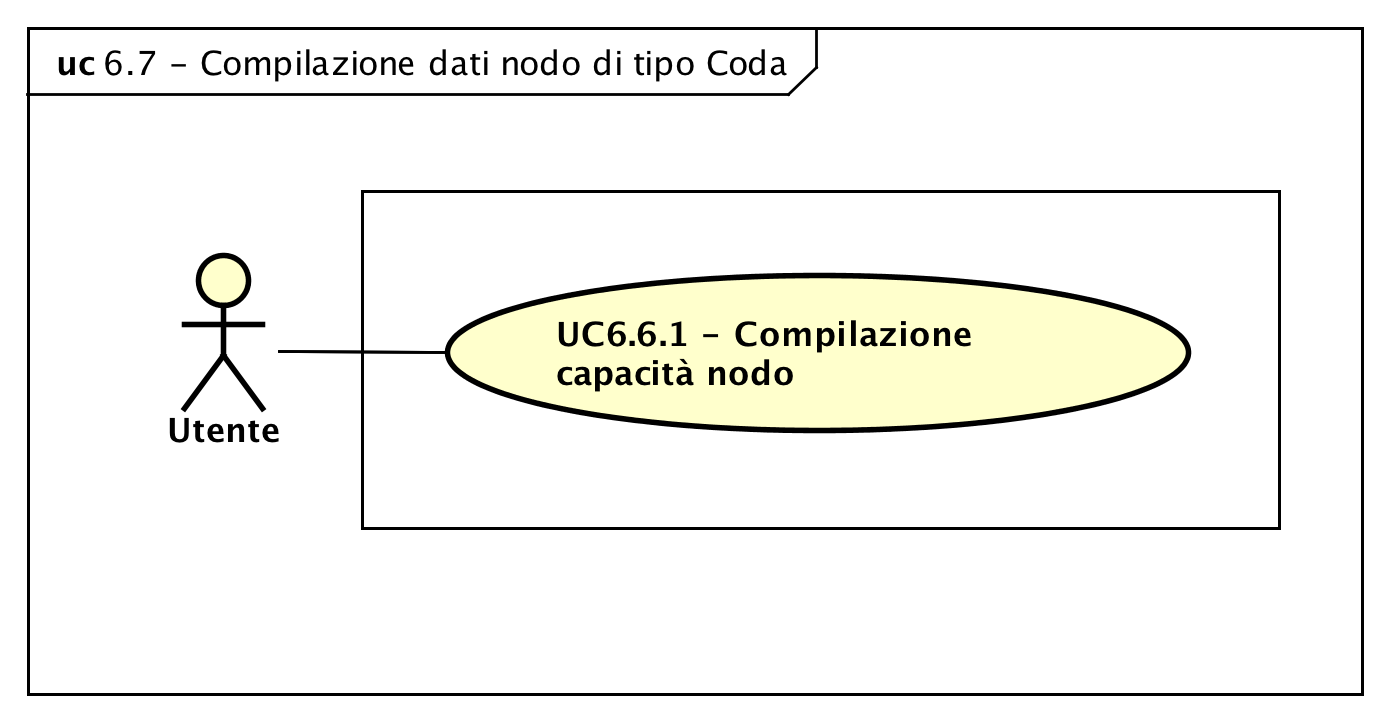
\includegraphics[scale=0.5]{{img/uc6.7}.png} 
	\caption{UC6.7 - Compilazione dati nodo di tipo Coda}
\end{figure}
\def\arraystretch{1.5}
\rowcolors{2}{D}{P}
\begin{tabularx}{\textwidth}{l|p{0.7\textwidth}}
	\rowcolor{I} \multicolumn{2}{c}{\color{white}\textbf{UC6.7 - Compilazione dati nodo di tipo Coda}} \\
	\toprule
	\endhead
	\textbf{Attori} & Utente\\
	\textbf{Descrizione} & l'utente compila i dati del nodo di tipo Coda\\
	\textbf{Pre-condizione} & l'utente ha posizionato il nodo; l'utente ha scelto come tipologia di nodo Coda\\
	\textbf{Post-condizione} & i dati del nodo di tipo Coda sono stati compilati; l'utente visualizza i dati appena compilati nell'area informativa\\
	\textbf{Scenario principale} & \vspace{-1.2em}\begin{enumerate}[leftmargin=*,noitemsep,nosep]
		\item \nameref{sssec:UC6.6.1}.
	\end{enumerate}\\
	%\textbf{Generalizzazioni} &  \\
	\bottomrule
\end{tabularx}
\subsection{UC6.8 - Compilazione dati nodo di tipo Sorgente} 
\label{sssec:UC6.8} 
\begin{figure}[H] 
	\centering 
	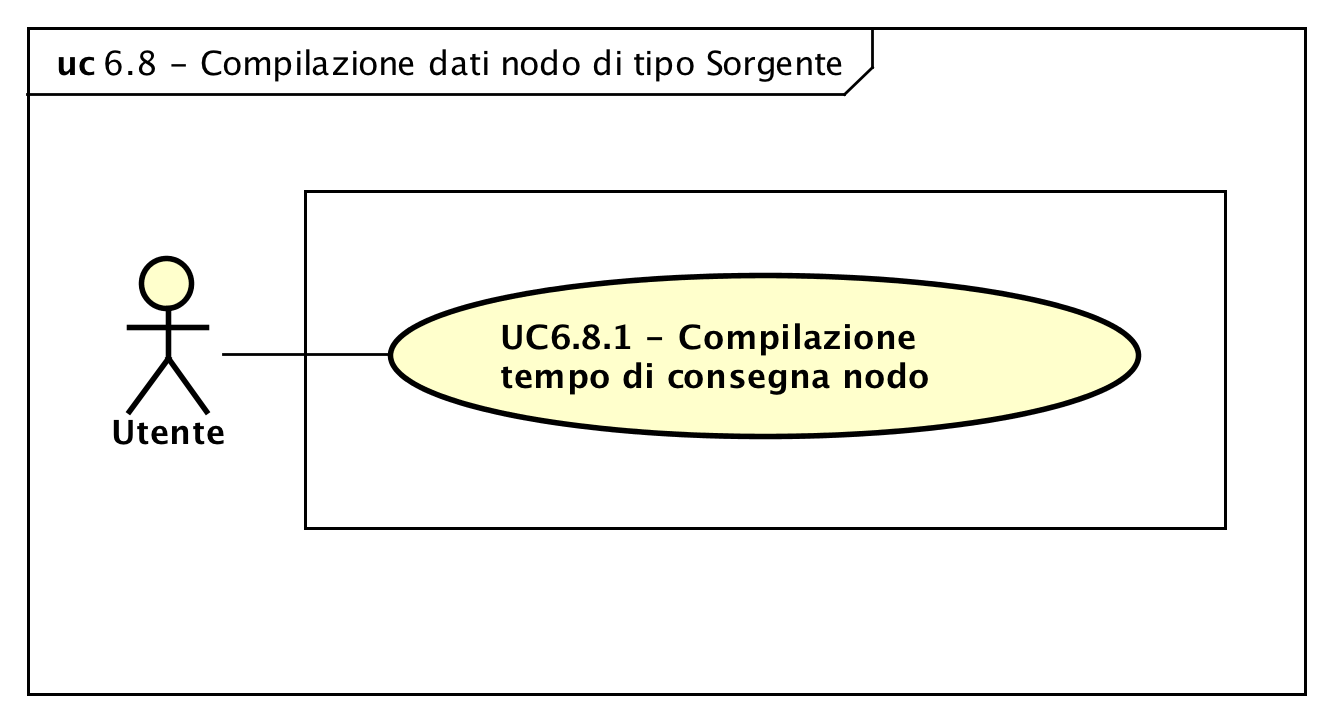
\includegraphics[scale=0.5]{{img/uc6.8}.png} 
	\caption{UC6.8 - Compilazione dati nodo di tipo Sorgente}
\end{figure}
\def\arraystretch{1.5}
\rowcolors{2}{D}{P}
\begin{tabularx}{\textwidth}{l|p{0.7\textwidth}}
	\rowcolor{I} \multicolumn{2}{c}{\color{white}\textbf{UC6.8 - Compilazione dati nodo di tipo Sorgente}} \\
	\toprule
	\endhead
	\textbf{Attori} & Utente\\
	\textbf{Descrizione} & l'utente compila i dati del nodo di tipo Sorgente\\
	\textbf{Pre-condizione} & l'utente ha posizionato il nodo; l'utente ha scelto come tipologia di nodo Sorgente\\
	\textbf{Post-condizione} & i dati del nodo di tipo Sorgente sono stati compilati; l'utente visualizza i dati appena compilati nell'area informativa\\
	\textbf{Scenario principale} & \vspace{-1.2em}\begin{enumerate}[leftmargin=*,noitemsep,nosep]
		\item \nameref{sssec:UC6.8.1}.
	\end{enumerate}\\
	%\textbf{Generalizzazioni} &  \\
	\bottomrule
\end{tabularx}
\subsection{UC6.8.1 - Compilazione tempo di consegna nodo} 
\label{sssec:UC6.8.1} 
\def\arraystretch{1.5}
\rowcolors{2}{D}{P}
\begin{tabularx}{\textwidth}{l|p{0.7\textwidth}}
	\rowcolor{I} \multicolumn{2}{c}{\color{white}\textbf{UC6.8.1 - Compilazione tempo di consegna nodo}} \\
	\toprule
	\endhead
	\textbf{Attori} & Utente\\
	\textbf{Descrizione} & l'utente compila il tempo di consegna del nodo\\
	\textbf{Pre-condizione} & il sistema offre la possibilità di compilare il tempo di consegna del nodo; l'utente ha scelto come tipologia di nodo Sorgente\\
	\textbf{Post-condizione} & l'utente ha compilato il tempo di consegna del nodo e visualizza il tempo appena compilato nell'area informativa\\
	\textbf{Scenario principale} & \vspace{-1.2em}\begin{enumerate}[leftmargin=*,noitemsep,nosep]
		\item \nameref{sssec:UC6.8.1}.
	\end{enumerate}\\
	%\textbf{Generalizzazioni} &  \\
	\bottomrule
\end{tabularx}
\subsection{UC6.9 - Compilazione dati nodo di tipo Risorsa} 
\label{sssec:UC6.9} 
\def\arraystretch{1.5}
\rowcolors{2}{D}{P}
\begin{tabularx}{\textwidth}{l|p{0.7\textwidth}}
	\rowcolor{I} \multicolumn{2}{c}{\color{white}\textbf{UC6.9 - Compilazione dati nodo di tipo Risorsa}} \\
	\toprule
	\endhead
	\textbf{Attori} & Utente\\
	\textbf{Descrizione} & l'utente compila i dati del nodo di tipo Risorsa\\
	\textbf{Pre-condizione} & l'utente ha posizionato il nodo; l'utente ha scelto come tipologia di nodo Risorsa\\
	\textbf{Post-condizione} & i dati del nodo di tipo Risorsa sono stati compilati; l'utente visualizza i dati appena compilati nell'area informativa\\
	\textbf{Scenario principale} & \vspace{-1.2em}\begin{enumerate}[leftmargin=*,noitemsep,nosep]
		\item \nameref{sssec:UC6.9}.
	\end{enumerate}\\
	%\textbf{Generalizzazioni} &  \\
	\bottomrule
\end{tabularx}
\subsection{UC6.10 - Conferma aggiunta nodo} 
\label{sssec:UC6.10} 
\def\arraystretch{1.5}
\rowcolors{2}{D}{P}
\begin{tabularx}{\textwidth}{l|p{0.7\textwidth}}
	\rowcolor{I} \multicolumn{2}{c}{\color{white}\textbf{UC6.10 - Conferma aggiunta nodo}} \\
	\toprule
	\endhead
	\textbf{Attori} & Utente\\
	\textbf{Descrizione} & l'utente conferma l'aggiunta di un nodo\\
	\textbf{Pre-condizione} & il sistema offre la possibilità di confermare l'aggiunta di un nodo\\
	\textbf{Post-condizione} & un nuovo nodo è stato aggiunto ed è visualizzabile sulla mappa; l'utente visualizza un messaggio che comunica la corretta esecuzione dell'operazione; l'area informativa rimane impostata sul nodo appena inserito; la posizione e il livello di ingrandimento della mappa rimangono invariati\\
	\textbf{Scenario principale} & \vspace{-1.2em}\begin{enumerate}[leftmargin=*,noitemsep,nosep]
		\item \nameref{sssec:UC6.10}.
	\end{enumerate}\\
	\textbf{Estensioni} & \vspace{-1.2em}\begin{itemize}[leftmargin=*,noitemsep,nosep]
		\item \nameref{sssec:UC6.11}: dati inseriti non validi:
		\begin{itemize}
			\item classe non scelta;
			\item nome vuoto; più lungo di 50 caratteri; inizia e/o finisce con uno spazio; contiene caratteri speciali;
			\item capacità vuota; più lunga di 5
			cifre per la parte intera; più di 2 per la parte decimale;
			\item tempo di processo vuoto; più lungo di 5 cifre per la parte intera; più di 2 per la parte decimale.
			\item valore (monetario) vuoto; più lungo di 20 cifre per la parte intera; più di 2 per la parte decimale;
			\item tempo di consegna vuoto; più lungo di 5 cifre per la parte intera; più di 2 per la parte decimale.
		\end{itemize}
	\end{itemize}\\
	%\textbf{Generalizzazioni} &  \\
	\bottomrule
\end{tabularx}
\subsection{UC6.11 - Visualizzazione errore aggiunta nodo} 
\label{sssec:UC6.11} 
\def\arraystretch{1.5}
\rowcolors{2}{D}{P}
\begin{tabularx}{\textwidth}{l|p{0.7\textwidth}}
	\rowcolor{I} \multicolumn{2}{c}{\color{white}\textbf{UC6.11 - Visualizzazione errore aggiunta nodo}} \\
	\toprule
	\endhead
	\textbf{Attori} & Utente\\
	\textbf{Descrizione} & l'utente visualizza un errore relativo ai dati del nodo compilati in modo errato\\
	\textbf{Pre-condizione} & l'utente sta tentando di inserire un nuovo nodo\\
	\textbf{Post-condizione} & nessun nuovo nodo aggiunto; l'utente visualizza un errore relativo ai dati del nodo compilati in modo errato; l'utente viene riportato alla schermata di aggiunta nodo\\
	\textbf{Scenario principale} & \vspace{-1.2em}\begin{enumerate}[leftmargin=*,noitemsep,nosep]
		\item \nameref{sssec:UC6.11}.
	\end{enumerate}\\
	%\textbf{Generalizzazioni} &  \\
	\bottomrule
\end{tabularx}
\subsection{UC7 - Visualizzazione info nodo} 
\label{sssec:UC7} 
\def\arraystretch{1.5}
\rowcolors{2}{D}{P}
\begin{tabularx}{\textwidth}{l|p{0.7\textwidth}}
	\rowcolor{I} \multicolumn{2}{c}{\color{white}\textbf{UC7 - Visualizzazione info nodo}} \\
	\toprule
	\endhead
	\textbf{Attori} & Utente\\
	\textbf{Descrizione} & l'utente seleziona un nodo e ne visualizza le informazioni\\
	\textbf{Pre-condizione} & l'utente ha aperto l'applicazione; è stato inserito almeno un nodo\\
	\textbf{Post-condizione} & il sistema mostra nell'area informativa le informazioni del nodo selezionato; la posizione e il livello di ingrandimento della mappa rimangono invariati\\
	\textbf{Scenario principale} & \vspace{-1.2em}\begin{enumerate}[leftmargin=*,noitemsep,nosep]
		\item \nameref{sssec:UC7}.
	\end{enumerate}\\
	%\textbf{Generalizzazioni} &  \\
	\bottomrule
\end{tabularx}
\subsection{UC8 - Chiusura visualizzazione info nodo} 
\label{sssec:UC8} 
\def\arraystretch{1.5}
\rowcolors{2}{D}{P}
\begin{tabularx}{\textwidth}{l|p{0.7\textwidth}}
	\rowcolor{I} \multicolumn{2}{c}{\color{white}\textbf{UC8 - Chiusura visualizzazione info nodo}} \\
	\toprule
	\endhead
	\textbf{Attori} & Utente\\
	\textbf{Descrizione} & l'utente chiude la visualizzazione delle informazioni di un nodo\\
	\textbf{Pre-condizione} & l'utente ha visualizzato le informazioni di un nodo\\
	\textbf{Post-condizione} & è stata chiusa la visualizzazione delle informazioni del nodo selezionato nell'area informativa; l'area informativa viene impostata sulla visualizzazione di default; la posizione e il livello di ingrandimento della mappa rimangono invariati\\
	\textbf{Scenario principale} & \vspace{-1.2em}\begin{enumerate}[leftmargin=*,noitemsep,nosep]
		\item \nameref{sssec:UC8}.
	\end{enumerate}\\
	%\textbf{Generalizzazioni} &  \\
	\bottomrule
\end{tabularx}
\subsection{UC9 - Modifica nodo} 
\label{sssec:UC9} 
\begin{figure}[H] 
	\centering 
	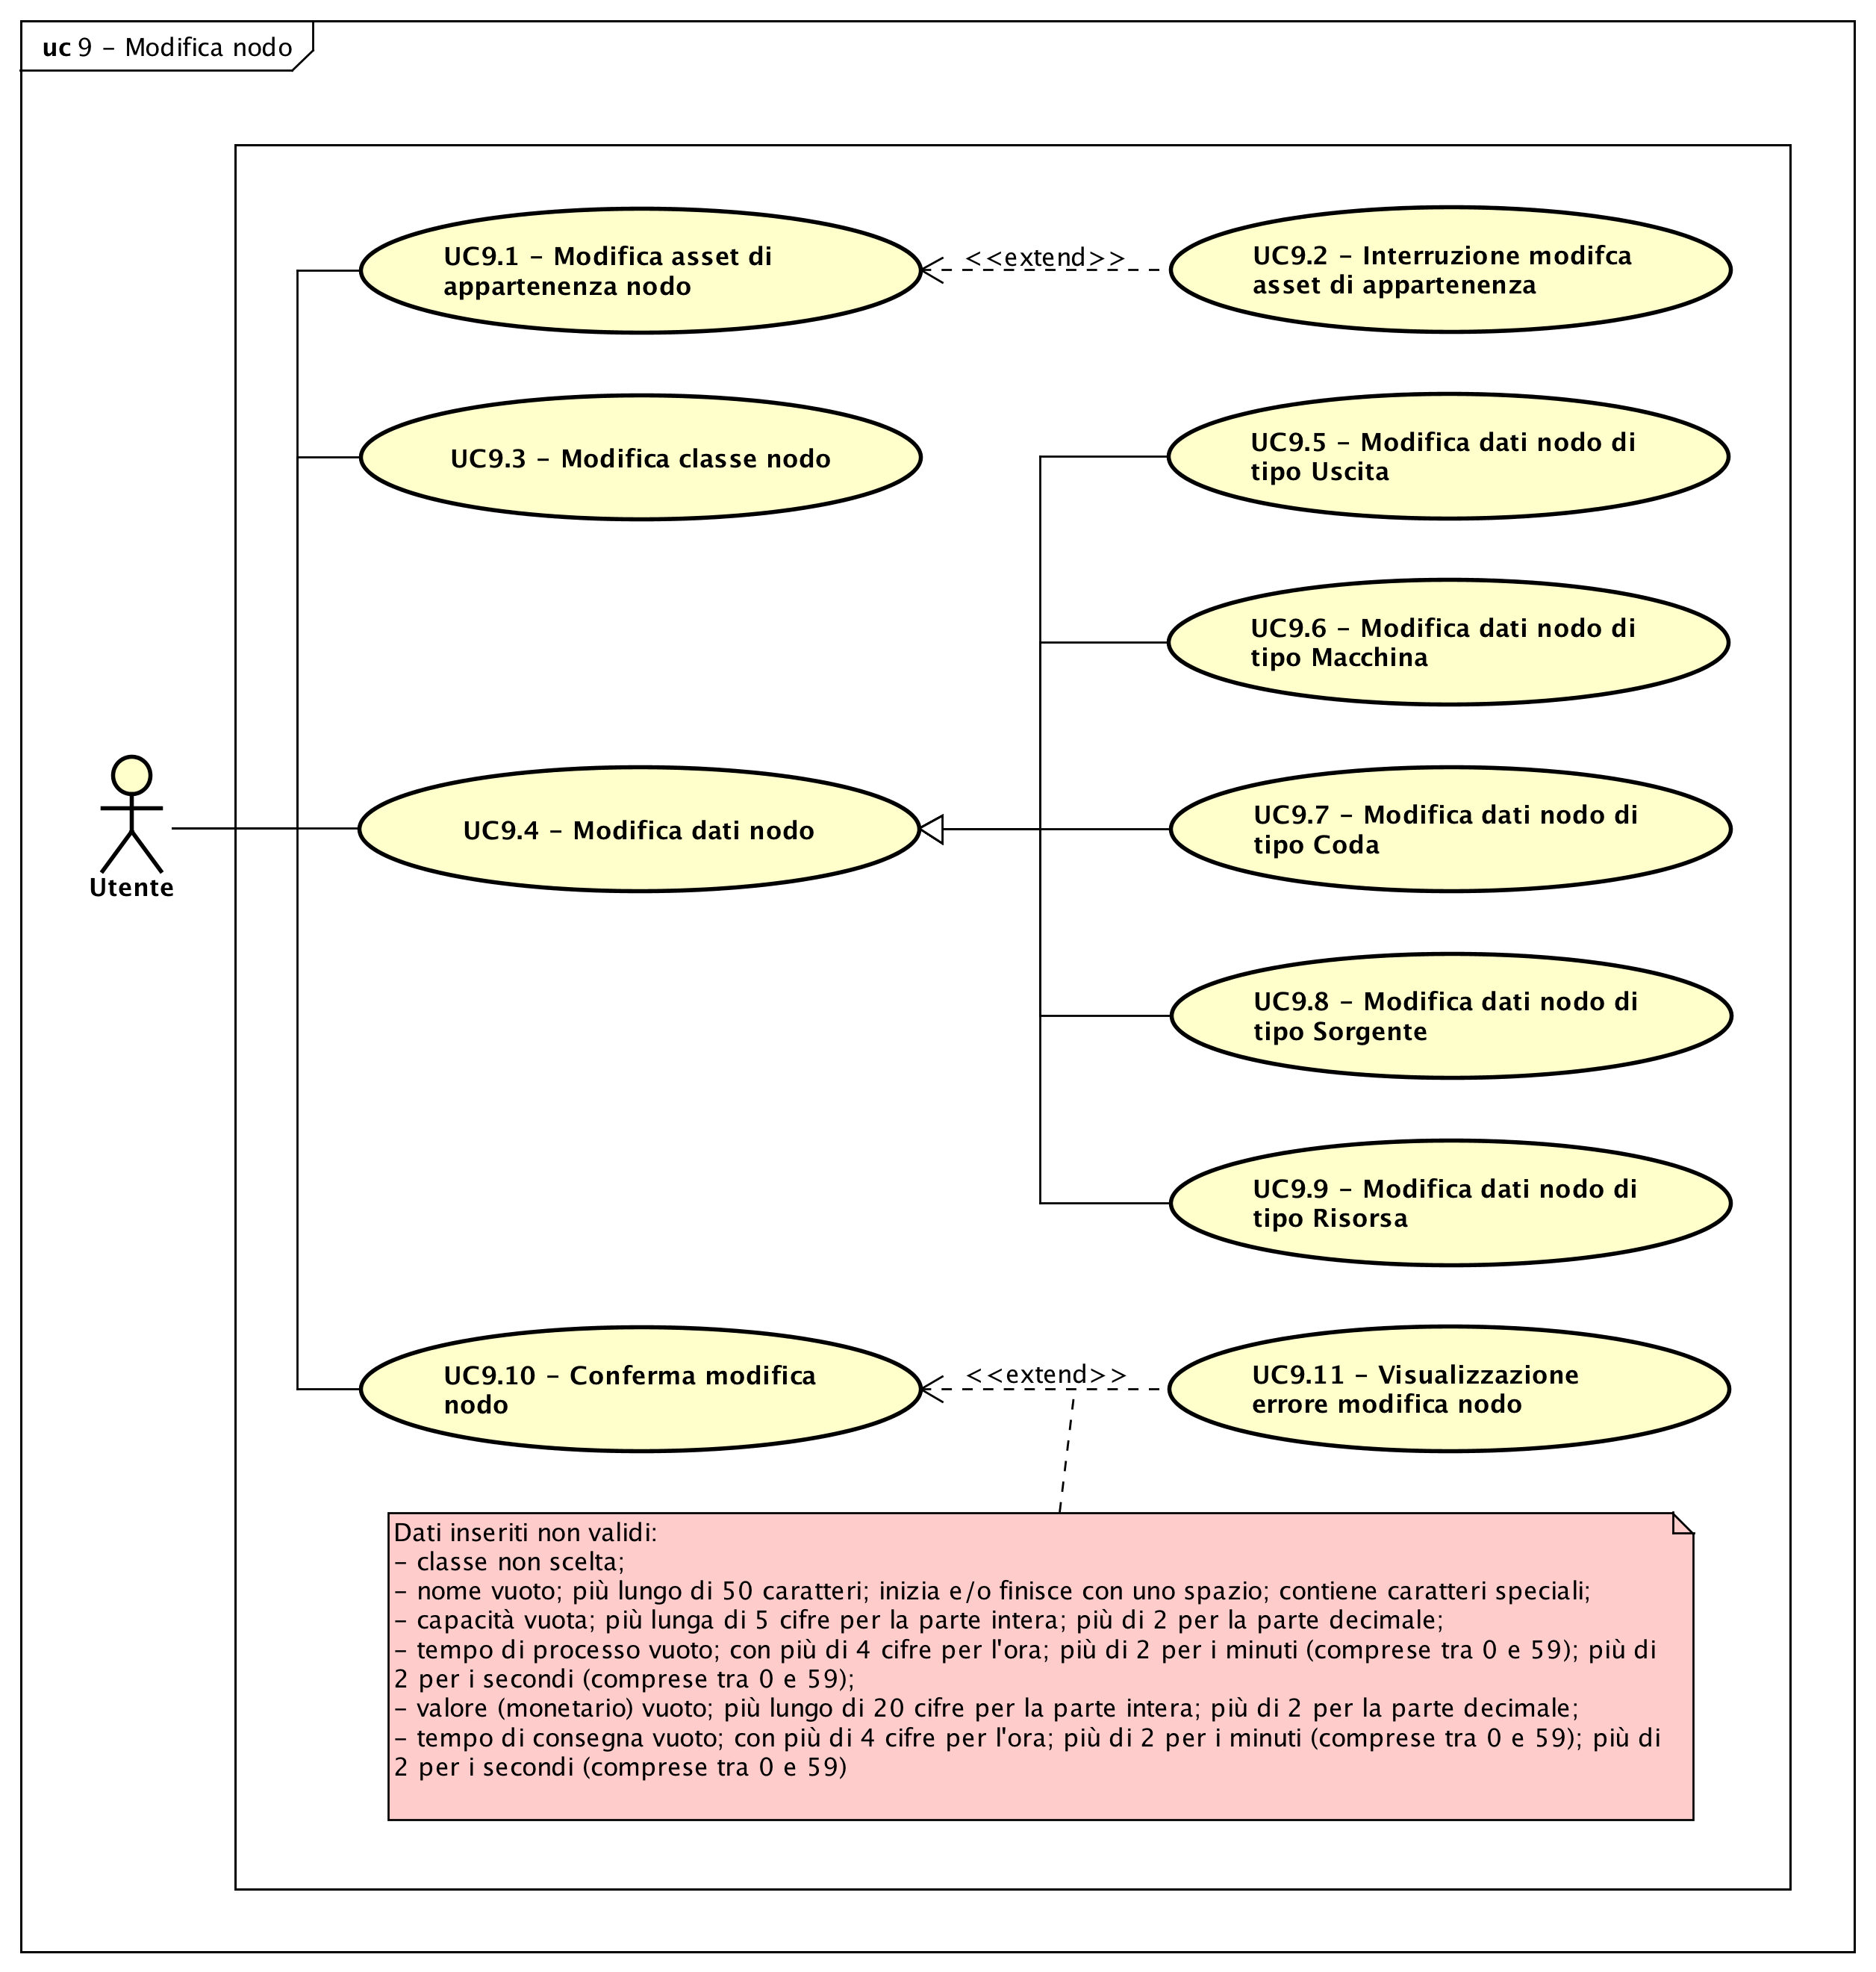
\includegraphics[width=\textwidth]{{img/uc9}.png} 
	\caption{UC9 - Modifica nodo}
\end{figure}
\def\arraystretch{1.5}
\rowcolors{2}{D}{P}
\begin{tabularx}{\textwidth}{l|p{0.7\textwidth}}
	\rowcolor{I} \multicolumn{2}{c}{\color{white}\textbf{UC9 - Modifica nodo}} \\
	\toprule
	\endhead
	\textbf{Attori} & Utente\\
	\textbf{Descrizione} & l'utente modifica il nodo\\
	\textbf{Pre-condizione} & l'utente ha aperto l'applicazione; almeno un nodo è stato aggiunto; l'utente ha selezionato un nodo\\
	\textbf{Post-condizione} & il nodo è stato modificato; l'utente visualizza un messaggio che comunica la corretta esecuzione dell'operazione; l'area informativa rimane impostata sul nodo appena modificato; la posizione e il livello di ingrandimento della mappa rimangono invariati\\
	\textbf{Scenario principale} & \vspace{-1.2em}\begin{enumerate}[leftmargin=*,noitemsep,nosep]
		\item \nameref{sssec:UC9.1};
		\item \nameref{sssec:UC9.2};
		\item \nameref{sssec:UC9.3};
		\item \nameref{sssec:UC9.4};
		\item \nameref{sssec:UC9.5} oppure
		\item \nameref{sssec:UC9.6} oppure
		\item \nameref{sssec:UC9.7} oppure
		\item \nameref{sssec:UC9.8} oppure
		\item \nameref{sssec:UC9.9};
		\item \nameref{sssec:UC9.10}.
	\end{enumerate}\\
	\textbf{Estensioni} & \vspace{-1.2em}\begin{itemize}[leftmargin=*,noitemsep,nosep]
		\item \nameref{sssec:UC34}.
	\end{itemize}\\
	\textbf{Scenari alternativi} & \vspace{-1.2em}\begin{itemize}[leftmargin=*,noitemsep,nosep]
		\item \nameref{sssec:UC9.11}.
	\end{itemize}\\
	%\textbf{Generalizzazioni} &  \\
	\bottomrule
\end{tabularx}
\subsection{UC9.1 - Modifica asset di appartenenza nodo} 
\label{sssec:UC9.1} 
\begin{figure}[H] 
	\centering 
	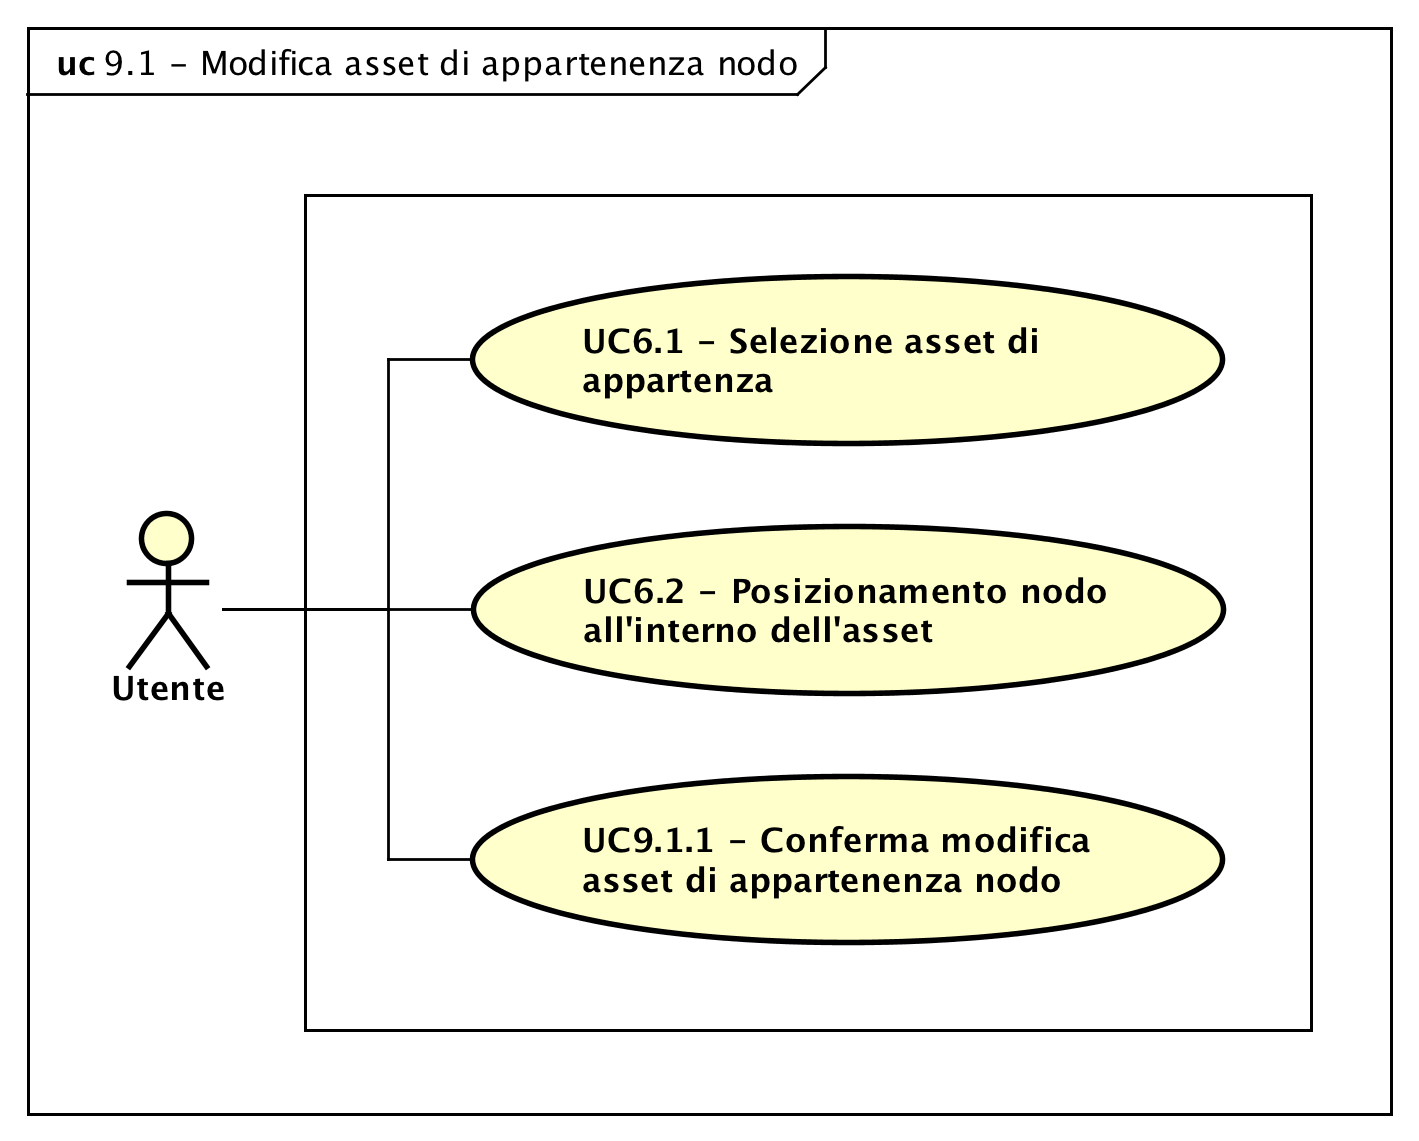
\includegraphics[scale=0.5]{{img/uc9.1}.png} 
	\caption{UC9.1 - Modifica asset di appartenenza nodo}
\end{figure}
\def\arraystretch{1.5}
\rowcolors{2}{D}{P}
\begin{tabularx}{\textwidth}{l|p{0.7\textwidth}}
	\rowcolor{I} \multicolumn{2}{c}{\color{white}\textbf{UC9.1 - Modifica asset di appartenenza nodo}} \\
	\toprule
	\endhead
	\textbf{Attori} & Utente\\
	\textbf{Descrizione} & l'utente modifica l'asset di appartenenza del nodo\\
	\textbf{Pre-condizione} & il sistema offre la possibilità di modificare l'asset di appartenenza del nodo\\
	\textbf{Post-condizione} & l'asset di appartenenza del nodo è stato modificato; il nodo viene spostato dal vecchio asset al nuovo ed è visualizzabile sulla mappa; l'utente può continuare a modificare altri dati del nodo\\
	\textbf{Scenario principale} & \vspace{-1.2em}\begin{enumerate}[leftmargin=*,noitemsep,nosep]
		\item \nameref{sssec:UC6.1}
		\item \nameref{sssec:UC6.2};
		\item \nameref{sssec:UC9.1.1}.
	\end{enumerate}\\
	\textbf{Estensioni} & \vspace{-1.2em}\begin{itemize}[leftmargin=*,noitemsep,nosep]
		\item \nameref{sssec:UC9.2}: l'utente interrompe volontariamente la modifica dell'asset di appartenenza del nodo
	\end{itemize}\\
	%\textbf{Generalizzazioni} &  \\
	\bottomrule
\end{tabularx}
\subsection{UC9.1.1 - Conferma modifica asset di appartenenza nodo} 
\label{sssec:UC9.1.1} 
\def\arraystretch{1.5}
\rowcolors{2}{D}{P}
\begin{tabularx}{\textwidth}{l|p{0.7\textwidth}}
	\rowcolor{I} \multicolumn{2}{c}{\color{white}\textbf{UC9.1.1 - Conferma modifica asset di appartenenza nodo}} \\
	\toprule
	\endhead
	\textbf{Attori} & Utente\\
	\textbf{Descrizione} & l'utente conferma la modifica dell'asset di appartenenza del nodo\\
	\textbf{Pre-condizione} & il sistema offre la possibilità di confermare l'asset di appartenenza del nodo\\
	\textbf{Post-condizione} & l'asset di appartenenza del nodo è stato modificato; il nodo viene spostato dall'asset che lo conteneva precedentemente al nuovo asset di appartenenza; l'utente può continuare a modificare altri dati del nodo\\
	\textbf{Scenario principale} & \vspace{-1.2em}\begin{enumerate}[leftmargin=*,noitemsep,nosep]
		\item \nameref{sssec:UC9.1.1}.
	\end{enumerate}\\
	%\textbf{Generalizzazioni} &  \\
	\bottomrule
\end{tabularx}

\subsection{UC9.2 - Interruzione modifica asset di appartenenza} 
\label{sssec:UC9.2} 
\def\arraystretch{1.5}
\rowcolors{2}{D}{P}
\begin{tabularx}{\textwidth}{l|p{0.7\textwidth}}
	\rowcolor{I} \multicolumn{2}{c}{\color{white}\textbf{UC9.2 - Interruzione modifica asset di appartenenza}} \\
	\toprule
	\endhead
	\textbf{Attori} & Utente\\
	\textbf{Descrizione} & l'utente interrompe la modifica dell'asset di appartenenza del nodo\\
	\textbf{Pre-condizione} & il sistema offre la possibilità di modificare l'asset di appartenenza\\
	\textbf{Post-condizione} & l'asset di appartenenza del nodo non è stato modificato; l'utente viene riportato alla schermata di modifica nodo e può modificarne altri dati\\
	\textbf{Scenario principale} & \vspace{-1.2em}\begin{enumerate}[leftmargin=*,noitemsep,nosep]
		\item \nameref{sssec:UC9.2}.
	\end{enumerate}\\
	%\textbf{Generalizzazioni} &  \\
	\bottomrule
\end{tabularx}
\subsection{UC9.3 - Modifica classe nodo} 
\label{sssec:UC9.3} 
\def\arraystretch{1.5}
\rowcolors{2}{D}{P}
\begin{tabularx}{\textwidth}{l|p{0.7\textwidth}}
	\rowcolor{I} \multicolumn{2}{c}{\color{white}\textbf{UC9.3 - Modifica classe nodo}} \\
	\toprule
	\endhead
	\textbf{Attori} & Utente\\
	\textbf{Descrizione} & l'utente modifica la classe del nodo\\
	\textbf{Pre-condizione} & il sistema offre la possibilità di modificare la classe del nodo\\
	\textbf{Post-condizione} & la classe del nodo è stata modificata; la forma del nodo sulla mappa cambia in base alla classe scelta\\
	\textbf{Scenario principale} & \vspace{-1.2em}\begin{enumerate}[leftmargin=*,noitemsep,nosep]
		\item \nameref{sssec:UC9.2}.
	\end{enumerate}\\
	%\textbf{Generalizzazioni} &  \\
	\bottomrule
\end{tabularx}
\subsection{UC9.4 - Modifica dati nodo} 
\label{sssec:UC9.4} 
\begin{figure}[H] 
	\centering 
	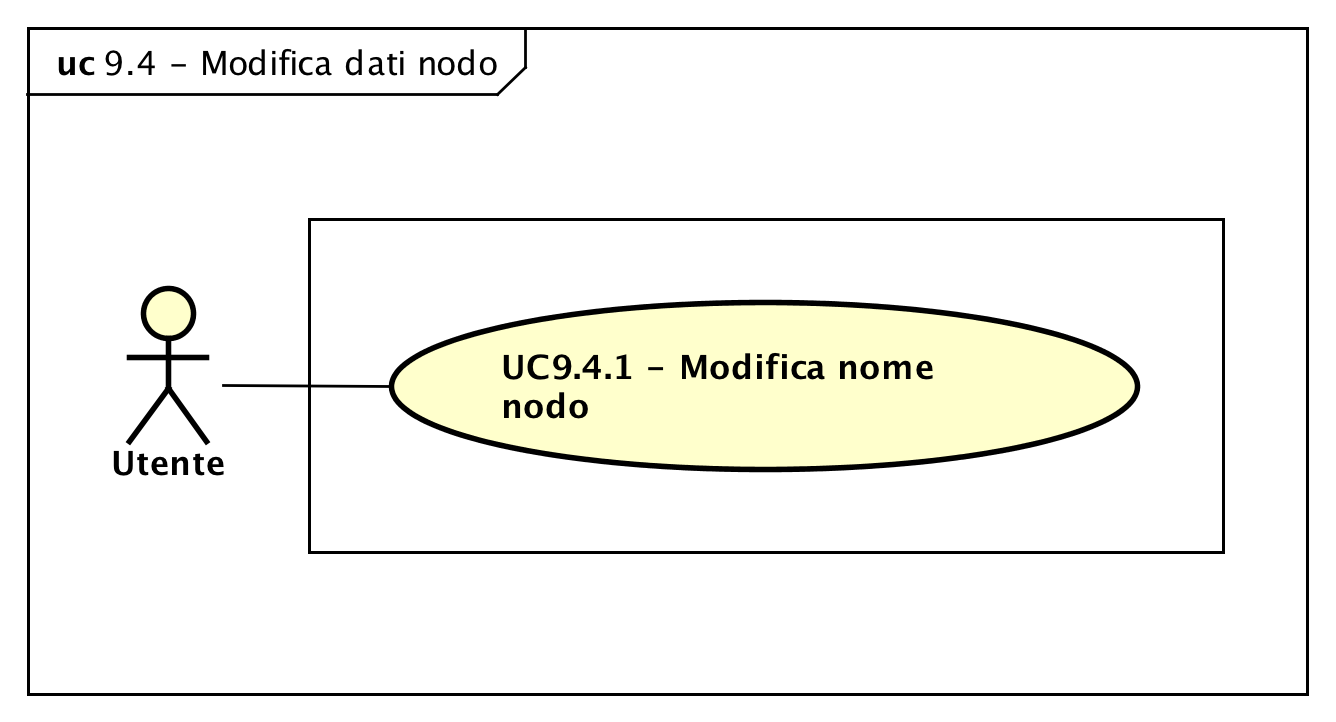
\includegraphics[scale=0.5]{{img/uc9.4}.png} 
	\caption{UC9.4 - Modifica dati nodo}
\end{figure}
\def\arraystretch{1.5}
\rowcolors{2}{D}{P}
\begin{tabularx}{\textwidth}{l|p{0.7\textwidth}}
	\rowcolor{I} \multicolumn{2}{c}{\color{white}\textbf{UC9.4 - Modifica dati nodo}} \\
	\toprule
	\endhead
	\textbf{Attori} & Utente\\
	\textbf{Descrizione} & l'utente modifica i dati del nodo\\
	\textbf{Pre-condizione} & il sistema offre la possibilità di modificare i dati del nodo;\\
	\textbf{Post-condizione} & i dati del nodo sono stati modificati; l'utente visualizza i dati appena modificati nell'area informativa\\
	\textbf{Scenario principale} & \vspace{-1.2em}\begin{enumerate}[leftmargin=*,noitemsep,nosep]
		\item \nameref{sssec:UC9.4.1}.
	\end{enumerate}\\
	\textbf{Generalizzazioni} &
	\vspace{-1.2em}\begin{itemize}
		[leftmargin=*,noitemsep,nosep]
		\item \nameref{sssec:UC9.5};
		\item \nameref{sssec:UC9.6};
		\item \nameref{sssec:UC9.7};
		\item \nameref{sssec:UC9.8};
		\item \nameref{sssec:UC9.9}.
	\end{itemize} \\
	\bottomrule
\end{tabularx}
\subsection{UC9.4.1 - Modifica nome nodo} 
\label{sssec:UC9.4.1} 
\def\arraystretch{1.5}
\rowcolors{2}{D}{P}
\begin{tabularx}{\textwidth}{l|p{0.7\textwidth}}
	\rowcolor{I} \multicolumn{2}{c}{\color{white}\textbf{UC9.4.1 - Modifica nome nodo}} \\
	\toprule
	\endhead
	\textbf{Attori} & Utente\\
	\textbf{Descrizione} & l'utente modifica il campo relativo al nome del nodo\\
	\textbf{Pre-condizione} & il sistema offre la possibilità di modificare il nome del nodo\\
	\textbf{Post-condizione} & il campo relativo al nome del nodo è stato modificato; l'utente visualizza il nome appena modificato nell'area informativa\\
	\textbf{Scenario principale} & \vspace{-1.2em}\begin{enumerate}[leftmargin=*,noitemsep,nosep]
		\item \nameref{sssec:UC9.4.1}.
	\end{enumerate}\\
	%\textbf{Generalizzazioni} &  \\
	\bottomrule
\end{tabularx}
\subsection{UC9.5 - Modifica dati nodo di tipo Uscita} 
\label{sssec:UC9.5} 
\def\arraystretch{1.5}
\rowcolors{2}{D}{P}
\begin{tabularx}{\textwidth}{l|p{0.7\textwidth}}
	\rowcolor{I} \multicolumn{2}{c}{\color{white}\textbf{UC9.5 - Modifica dati nodo di tipo Uscita}} \\
	\toprule
	\endhead
	\textbf{Attori} & Utente\\
	\textbf{Descrizione} & l'utente modifica i dati del nodo di tipo Uscita\\
	\textbf{Pre-condizione} & il sistema offre la possibilità di modificare i dati del nodo; l'utente ha scelto un nodo di tipo Uscita\\
	\textbf{Post-condizione} & i dati del nodo sono stati modificati; l'utente visualizza i dati appena modificati nell'area informativa\\
	\textbf{Scenario principale} & \vspace{-1.2em}\begin{enumerate}[leftmargin=*,noitemsep,nosep]
		\item \nameref{sssec:UC9.5}.
	\end{enumerate}\\
	%\textbf{Generalizzazioni} &  \\
	\bottomrule
\end{tabularx}
\subsection{UC9.6 - Modifica dati nodo di tipo Macchina} 
\label{sssec:UC9.6} 
\begin{figure}[H] 
	\centering 
	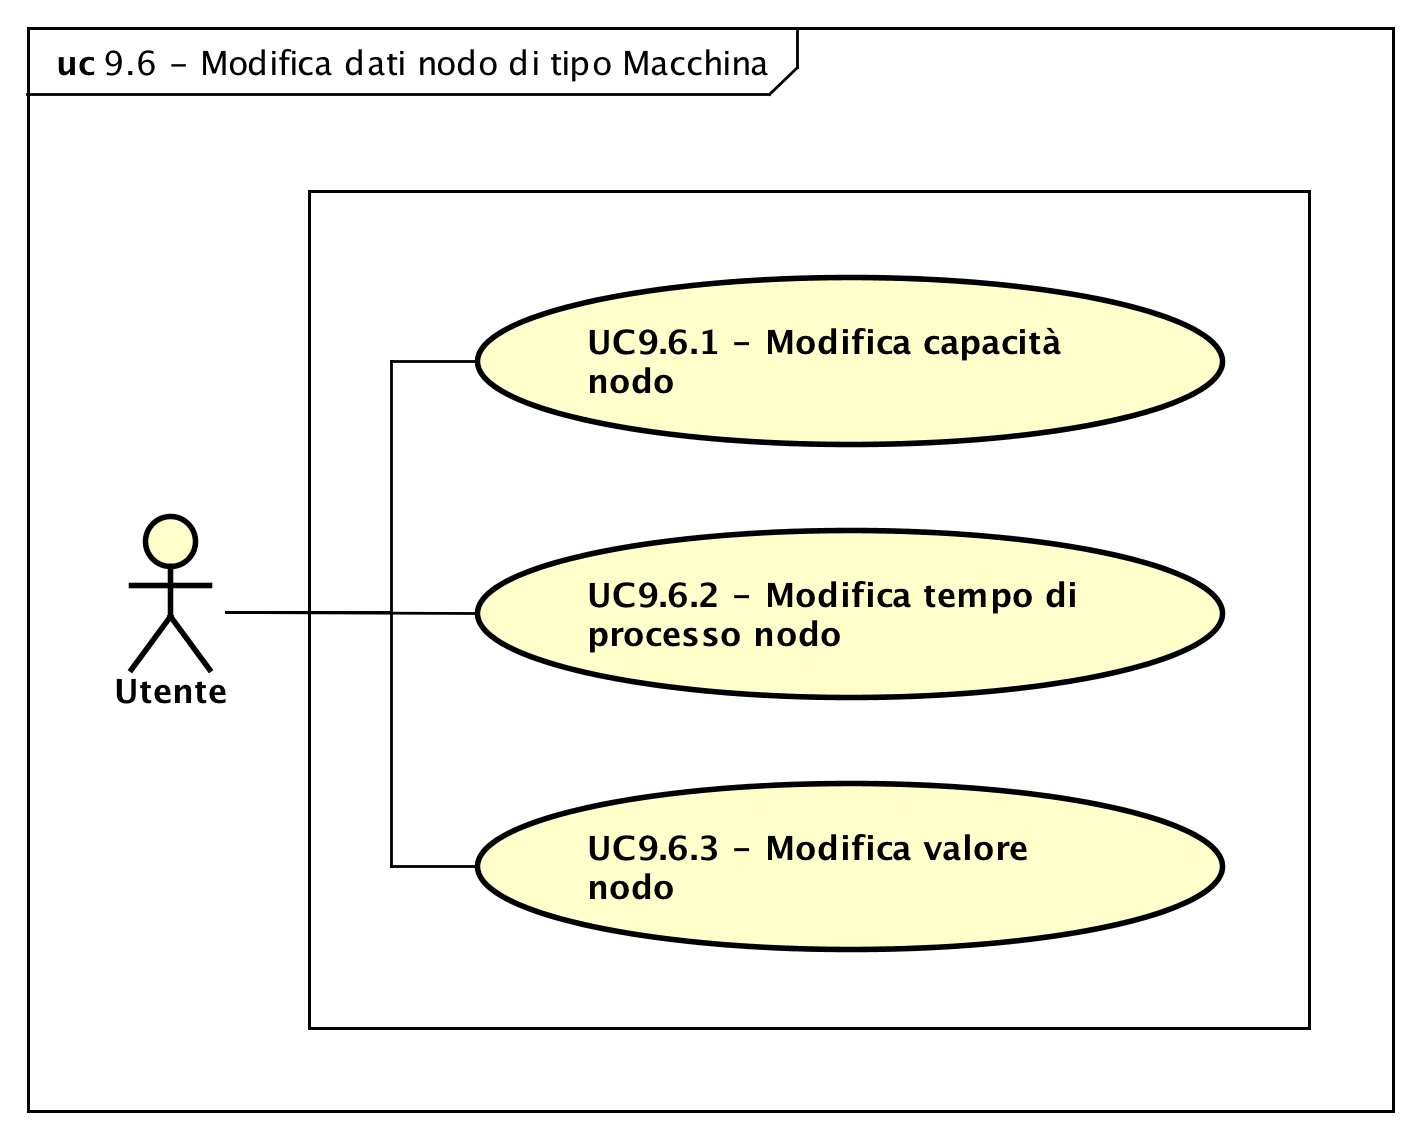
\includegraphics[scale=0.5]{{img/uc9.6}.png} 
	\caption{UC9.6 - Modifica dati nodo di tipo Macchina}
\end{figure}
\def\arraystretch{1.5}
\rowcolors{2}{D}{P}
\begin{tabularx}{\textwidth}{l|p{0.7\textwidth}}
	\rowcolor{I} \multicolumn{2}{c}{\color{white}\textbf{UC9.6 - Modifica dati nodo di tipo Macchina}} \\
	\toprule
	\endhead
	\textbf{Attori} & Utente\\
	\textbf{Descrizione} & l'utente modifica i dati del nodo di tipo Macchina\\
	\textbf{Pre-condizione} & il sistema offre la possibilità di modificare i dati del nodo; l'utente ha scelto un nodo di tipo Macchina\\
	\textbf{Post-condizione} & i dati del nodo sono stati modificati; l'utente visualizza i dati appena modificati nell'area informativa\\
	\textbf{Scenario principale} & \vspace{-1.2em}\begin{enumerate}[leftmargin=*,noitemsep,nosep]
		\item \nameref{sssec:UC9.6.1};
		\item \nameref{sssec:UC9.6.2};
		\item \nameref{sssec:UC9.6.3}.
	\end{enumerate}\\
	%\textbf{Generalizzazioni} &  \\
	\bottomrule
\end{tabularx}
\subsection{UC9.6.1 - Modifica capacità nodo} 
\label{sssec:UC9.6.1} 
\def\arraystretch{1.5}
\rowcolors{2}{D}{P}
\begin{tabularx}{\textwidth}{l|p{0.7\textwidth}}
	\rowcolor{I} \multicolumn{2}{c}{\color{white}\textbf{UC9.6.1 - Modifica capacità nodo}} \\
	\toprule
	\endhead
	\textbf{Attori} & Utente\\
	\textbf{Descrizione} & l'utente modifica il campo relativo alla capacità del nodo\\
	\textbf{Pre-condizione} & il sistema offre la possibilità di modificare la capacità del nodo; l'utente ha scelto come classe del nodo Macchina o Coda\\
	\textbf{Post-condizione} & il campo relativo alla capacità del nodo è stato modificato; l'utente visualizza la capacità del nodo appena modificata\\
	\textbf{Scenario principale} & \vspace{-1.2em}\begin{enumerate}[leftmargin=*,noitemsep,nosep]
		\item \nameref{sssec:UC9.6.1}.
	\end{enumerate}\\
	%\textbf{Generalizzazioni} &  \\
	\bottomrule
\end{tabularx}
\subsection{UC9.6.2 - Modifica tempo di processo nodo} 
\label{sssec:UC9.6.2} 
\def\arraystretch{1.5}
\rowcolors{2}{D}{P}
\begin{tabularx}{\textwidth}{l|p{0.7\textwidth}}
	\rowcolor{I} \multicolumn{2}{c}{\color{white}\textbf{UC9.6.2 - Modifica tempo di processo nodo}} \\
	\toprule
	\endhead
	\textbf{Attori} & Utente\\
	\textbf{Descrizione} & l'utente modifica il campo relativo al tempo di processo del nodo\\
	\textbf{Pre-condizione} & il sistema offre la possibilità di modificare il tempo di processo del nodo; l'utente ha scelto come classe del nodo Macchina\\
	\textbf{Post-condizione} & il campo relativo al tempo di processo del nodo è stato modificato; l'utente visualizza il tempo di processo appena modificato\\
	\textbf{Scenario principale} & \vspace{-1.2em}\begin{enumerate}[leftmargin=*,noitemsep,nosep]
		\item \nameref{sssec:UC9.6.2}.
	\end{enumerate}\\
	%\textbf{Generalizzazioni} &  \\
	\bottomrule
\end{tabularx}
\subsection{UC9.6.3 - Modifica valore nodo} 
\label{sssec:UC9.6.3} 
\def\arraystretch{1.5}
\rowcolors{2}{D}{P}
\begin{tabularx}{\textwidth}{l|p{0.7\textwidth}}
	\rowcolor{I} \multicolumn{2}{c}{\color{white}\textbf{UC9.6.3 - Modifica valore nodo}} \\
	\toprule
	\endhead
	\textbf{Attori} & Utente\\
	\textbf{Descrizione} & l'utente modifica il campo relativo al valore del nodo\\
	\textbf{Pre-condizione} & il sistema offre la possibilità di modificare il valore del nodo; l'utente ha scelto come classe del nodo Macchina\\
	\textbf{Post-condizione} & il campo relativo al valore del nodo è stato modificato; l'utente visualizza il valore appena modificato\\
	\textbf{Scenario principale} & \vspace{-1.2em}\begin{enumerate}[leftmargin=*,noitemsep,nosep]
		\item \nameref{sssec:UC9.6.3}.
	\end{enumerate}\\
	%\textbf{Generalizzazioni} &  \\
	\bottomrule
\end{tabularx}
\subsection{UC9.7 - Modifica dati nodo di tipo Coda} 
\label{sssec:UC9.7} 
\begin{figure}[H] 
	\centering 
	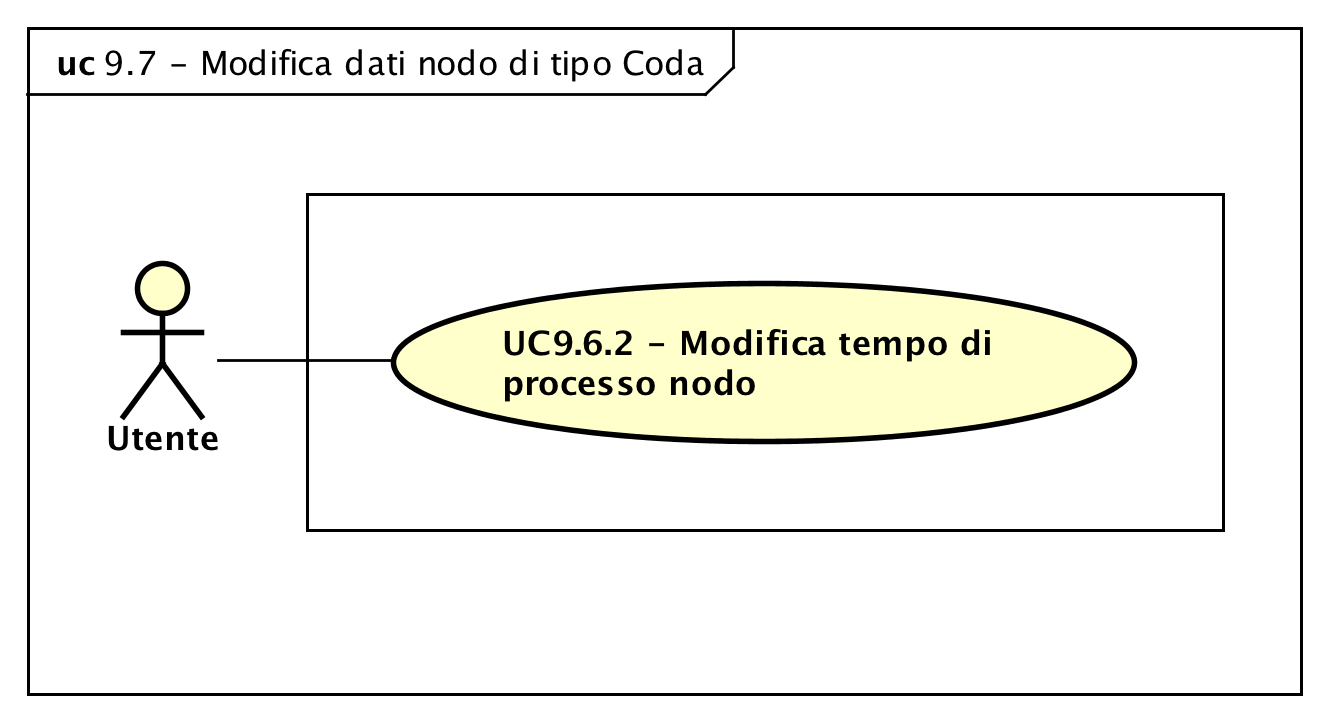
\includegraphics[scale=0.5]{{img/uc9.7}.png} 
	\caption{UC9.7 - Modifica dati nodo di tipo Coda}
\end{figure}
\def\arraystretch{1.5}
\rowcolors{2}{D}{P}
\begin{tabularx}{\textwidth}{l|p{0.7\textwidth}}
	\rowcolor{I} \multicolumn{2}{c}{\color{white}\textbf{UC9.7 - Modifica dati nodo di tipo Coda}} \\
	\toprule
	\endhead
	\textbf{Attori} & Utente\\
	\textbf{Descrizione} & l'utente modifica i dati del nodo di tipo Coda\\
	\textbf{Pre-condizione} & il sistema offre la possibilità di modificare i dati del nodo; l'utente ha scelto un nodo di tipo Coda\\
	\textbf{Post-condizione} & i dati del nodo sono stati modificati; l'utente visualizza i dati appena modificati nell'area informativa\\
	\textbf{Scenario principale} & \vspace{-1.2em}\begin{enumerate}[leftmargin=*,noitemsep,nosep]
		\item \nameref{sssec:UC9.6.2}.
	\end{enumerate}\\
	%\textbf{Generalizzazioni} &  \\
	\bottomrule
\end{tabularx}
\subsection{UC9.8 - Modifica dati nodo di tipo Sorgente} 
\label{sssec:UC9.8} 
\begin{figure}[H] 
	\centering 
	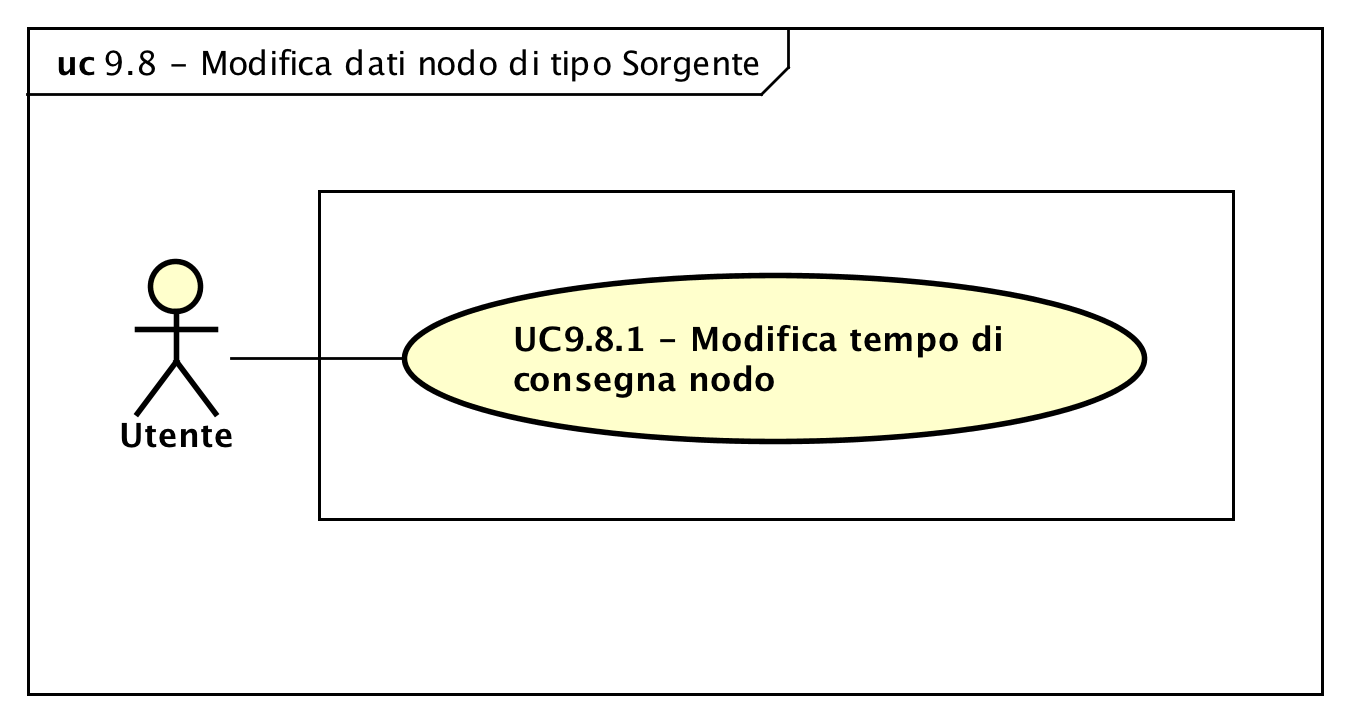
\includegraphics[scale=0.5]{{img/uc9.8}.png} 
	\caption{UC9.8 - Modifica dati nodo di tipo Sorgente}
\end{figure}
\def\arraystretch{1.5}
\rowcolors{2}{D}{P}
\begin{tabularx}{\textwidth}{l|p{0.7\textwidth}}
	\rowcolor{I} \multicolumn{2}{c}{\color{white}\textbf{UC9.8 - Modifica dati nodo di tipo Sorgente}} \\
	\toprule
	\endhead
	\textbf{Attori} & Utente\\
	\textbf{Descrizione} & l'utente modifica i dati del nodo di tipo Sorgente\\
	\textbf{Pre-condizione} & il sistema offre la possibilità di modificare i dati del nodo; l'utente ha scelto un nodo di tipo Sorgente\\
	\textbf{Post-condizione} & i dati del nodo sono stati modificati; l'utente visualizza i dati appena modificati nell'area informativa\\
	\textbf{Scenario principale} & \vspace{-1.2em}\begin{enumerate}[leftmargin=*,noitemsep,nosep]
		\item \nameref{sssec:UC9.8.1}.
	\end{enumerate}\\
	%\textbf{Generalizzazioni} &  \\
	\bottomrule
\end{tabularx}
\subsection{UC9.8.1 - Modifica tempo di consegna nodo} 
\label{sssec:UC9.8.1} 
\def\arraystretch{1.5}
\rowcolors{2}{D}{P}
\begin{tabularx}{\textwidth}{l|p{0.7\textwidth}}
	\rowcolor{I} \multicolumn{2}{c}{\color{white}\textbf{UC9.8.1 - Modifica tempo di consegna nodo}} \\
	\toprule
	\endhead
	\textbf{Attori} & Utente\\
	\textbf{Descrizione} & l'utente modifica il campo relativo al  tempo di consegna del nodo\\
	\textbf{Pre-condizione} & il sistema offre la possibilità di modificare il tempo di consegna del nodo; l'utente ha scelto come classe del nodo Sorgente\\
	\textbf{Post-condizione} & il campo relativo al tempo di consegna del nodo è stato modificato; l'utente visualizza il tempo di consegna appena modificato\\
	\textbf{Scenario principale} & \vspace{-1.2em}\begin{enumerate}[leftmargin=*,noitemsep,nosep]
		\item \nameref{sssec:UC9.8.1}.
	\end{enumerate}\\
	%\textbf{Generalizzazioni} &  \\
	\bottomrule
\end{tabularx}
\subsection{UC9.9 - Modifica dati nodo di tipo Risorsa} 
\label{sssec:UC9.9} 
\def\arraystretch{1.5}
\rowcolors{2}{D}{P}
\begin{tabularx}{\textwidth}{l|p{0.7\textwidth}}
	\rowcolor{I} \multicolumn{2}{c}{\color{white}\textbf{UC9.9 - Modifica dati nodo di tipo Risorsa}} \\
	\toprule
	\endhead
	\textbf{Attori} & Utente\\
	\textbf{Descrizione} & l'utente modifica i dati del nodo di tipo Risorsa\\
	\textbf{Pre-condizione} & il sistema offre la possibilità di modificare i dati del nodo; l'utente ha scelto un nodo di tipo Risorsa\\
	\textbf{Post-condizione} & i dati del nodo sono stati modificati; l'utente visualizza i dati appena modificati nell'area informativa\\
	\textbf{Scenario principale} & \vspace{-1.2em}\begin{enumerate}[leftmargin=*,noitemsep,nosep]
		\item \nameref{sssec:UC9.9}.
	\end{enumerate}\\
	%\textbf{Generalizzazioni} &  \\
	\bottomrule
\end{tabularx}
\subsection{UC9.10 - Conferma modifica nodo} 
\label{sssec:UC9.10} 
\def\arraystretch{1.5}
\rowcolors{2}{D}{P}
\begin{tabularx}{\textwidth}{l|p{0.7\textwidth}}
	\rowcolor{I} \multicolumn{2}{c}{\color{white}\textbf{UC9.10 - Conferma modifica nodo}} \\
	\toprule
	\endhead
	\textbf{Attori} & Utente\\
	\textbf{Descrizione} & l'utente conferma la modifica del nodo\\
	\textbf{Pre-condizione} & il sistema offre la possibilità di confermare la modifica del nodo\\
	\textbf{Post-condizione} & il nodo è stato modificato;  l'utente visualizza un messaggio che comunica la corretta esecuzione dell'operazione; l'area informativa rimane impostata sul nodo appena modificato; la posizione e il livello di ingrandimento della mappa rimangono invariati\\
	\textbf{Scenario principale} & \vspace{-1.2em}\begin{enumerate}[leftmargin=*,noitemsep,nosep]
		\item \nameref{sssec:UC9.10}.
	\end{enumerate}\\
	\textbf{Estensioni} & \vspace{-1.2em}\begin{itemize}[leftmargin=*,noitemsep,nosep]
		\item \nameref{sssec:UC9.11}: dati inseriti non validi:
		\begin{itemize}
			\item classe non scelta;
			\item nome vuoto; più lungo di 50
			caratteri; inizia e/o finisce con uno spazio; contiene caratteri
			speciali;
			\item capacità vuota; più lunga di 5
			cifre per la parte intera; più di 2 per la parte decimale;
			\item tempo di processo vuoto; più lungo di 5 cifre per la parte intera; più di 2 per la parte decimale.
			\item valore (monetario) vuoto; più
			lungo di 20 cifre per la parte intera; più di 2 per la parte
			decimale;
			\item tempo di consegna vuoto; più lungo di 5 cifre per la parte intera; più di 2 per la parte decimale.
		\end{itemize}
	\end{itemize}\\
	%\textbf{Generalizzazioni} &  \\
	\bottomrule
\end{tabularx}
\subsection{UC9.11 - Visualizzazione errore modifica nodo} 
\label{sssec:UC9.11} 
\def\arraystretch{1.5}
\rowcolors{2}{D}{P}
\begin{tabularx}{\textwidth}{l|p{0.7\textwidth}}
	\rowcolor{I} \multicolumn{2}{c}{\color{white}\textbf{UC9.11 - Visualizzazione errore modifica nodo}} \\
	\toprule
	\endhead
	\textbf{Attori} & Utente\\
	\textbf{Descrizione} & l'utente visualizza un errore relativo alla modifica del nodo\\
	\textbf{Pre-condizione} & l'utente ha confermato la modifica dei dati del nodo\\
	\textbf{Post-condizione} & il nodo non è stato modificato; l'utente visualizza un errore relativo ai dati del nodo compilati in modo errato; l'utente viene riportato alla schermata di modifica nodo\\
	\textbf{Scenario principale} & \vspace{-1.2em}\begin{enumerate}[leftmargin=*,noitemsep,nosep]
		\item \nameref{sssec:UC9.11}.
	\end{enumerate}\\
	%\textbf{Generalizzazioni} &  \\
	\bottomrule
\end{tabularx}
\subsection{UC10 - Eliminazione nodo} 
\label{sssec:UC10} 
\begin{figure}[H] 
	\centering 
	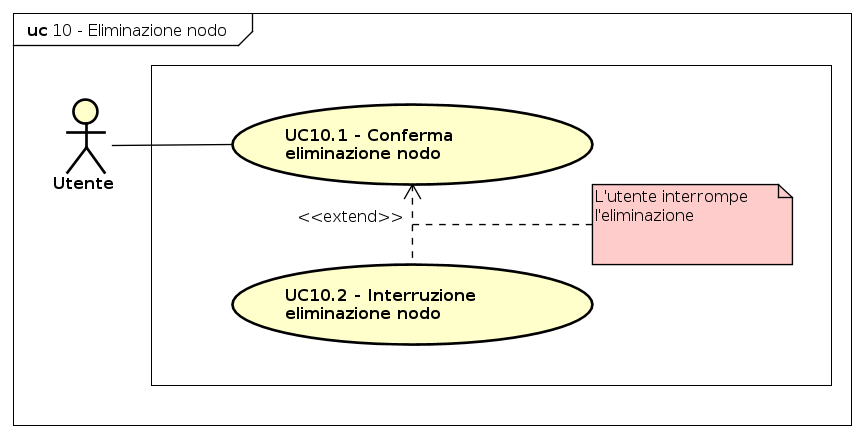
\includegraphics[scale=0.5]{{img/uc10}.png} 
	\caption{UC10 - Eliminazione nodo}
\end{figure}
\def\arraystretch{1.5}
\rowcolors{2}{D}{P}
\begin{tabularx}{\textwidth}{l|p{0.7\textwidth}}
	\rowcolor{I} \multicolumn{2}{c}{\color{white}\textbf{UC10 - Eliminazione nodo}} \\
	\toprule
	\endhead
	\textbf{Attori} & Utente\\
	\textbf{Descrizione} & l'utente elimina un nodo\\
	\textbf{Pre-condizione} & l'utente ha aperto l'applicazione; è stato inserito almeno un nodo; l'utente ha selezionato un nodo\\
	\textbf{Post-condizione} & il nodo è stato eliminato e non è più visibile sulla mappa; sono stati eliminati anche gli archi relativi a quel nodo; l'utente visualizza un messaggio che comunica la corretta esecuzione dell'operazione; l'area informativa viene impostata sulla visualizzazione di default;  la posizione e il livello di ingrandimento della mappa rimangono invariati\\
	\textbf{Scenario principale} & \vspace{-1.2em}\begin{enumerate}[leftmargin=*,noitemsep,nosep]
		\item \nameref{sssec:UC10.1}.
	\end{enumerate}\\
	\textbf{Estensioni} & \vspace{-1.2em}\begin{itemize}[leftmargin=*,noitemsep,nosep]
		\item \nameref{sssec:UC35}: l'utente interrompe volontariamente l'eliminazione del nodo
	\end{itemize}\\
	%\textbf{Generalizzazioni} &  \\
	\bottomrule
\end{tabularx}
\subsection{UC10.1 - Conferma eliminazione nodo} 
\label{sssec:UC10.1} 
\def\arraystretch{1.5}
\rowcolors{2}{D}{P}
\begin{tabularx}{\textwidth}{l|p{0.7\textwidth}}
	\rowcolor{I} \multicolumn{2}{c}{\color{white}\textbf{UC10.1 - Conferma eliminazione nodo}} \\
	\toprule
	\endhead
	\textbf{Attori} & Utente\\
	\textbf{Descrizione} & l'utente conferma l'eliminazione del nodo\\
	\textbf{Pre-condizione} & il sistema offre la possibilità di confermare l'eliminazione del nodo\\
	\textbf{Post-condizione} & il nodo è stato eliminato e non è più visibile sulla mappa; sono stati eliminati anche gli archi relativi a quel nodo; l'utente visualizza un messaggio che comunica la corretta esecuzione dell'operazione; l'area informativa viene impostata sulla visualizzazione di default;  la posizione e il livello di ingrandimento della mappa rimangono invariati\\
	\textbf{Scenario principale} & \vspace{-1.2em}\begin{enumerate}[leftmargin=*,noitemsep,nosep]
		\item \nameref{sssec:UC10.1}.
	\end{enumerate}\\
	%\textbf{Generalizzazioni} &  \\
	\bottomrule
\end{tabularx}
\subsection{UC11 - Aggiunta arco} 
\label{sssec:UC11} 
\begin{figure}[H] 
	\centering 
	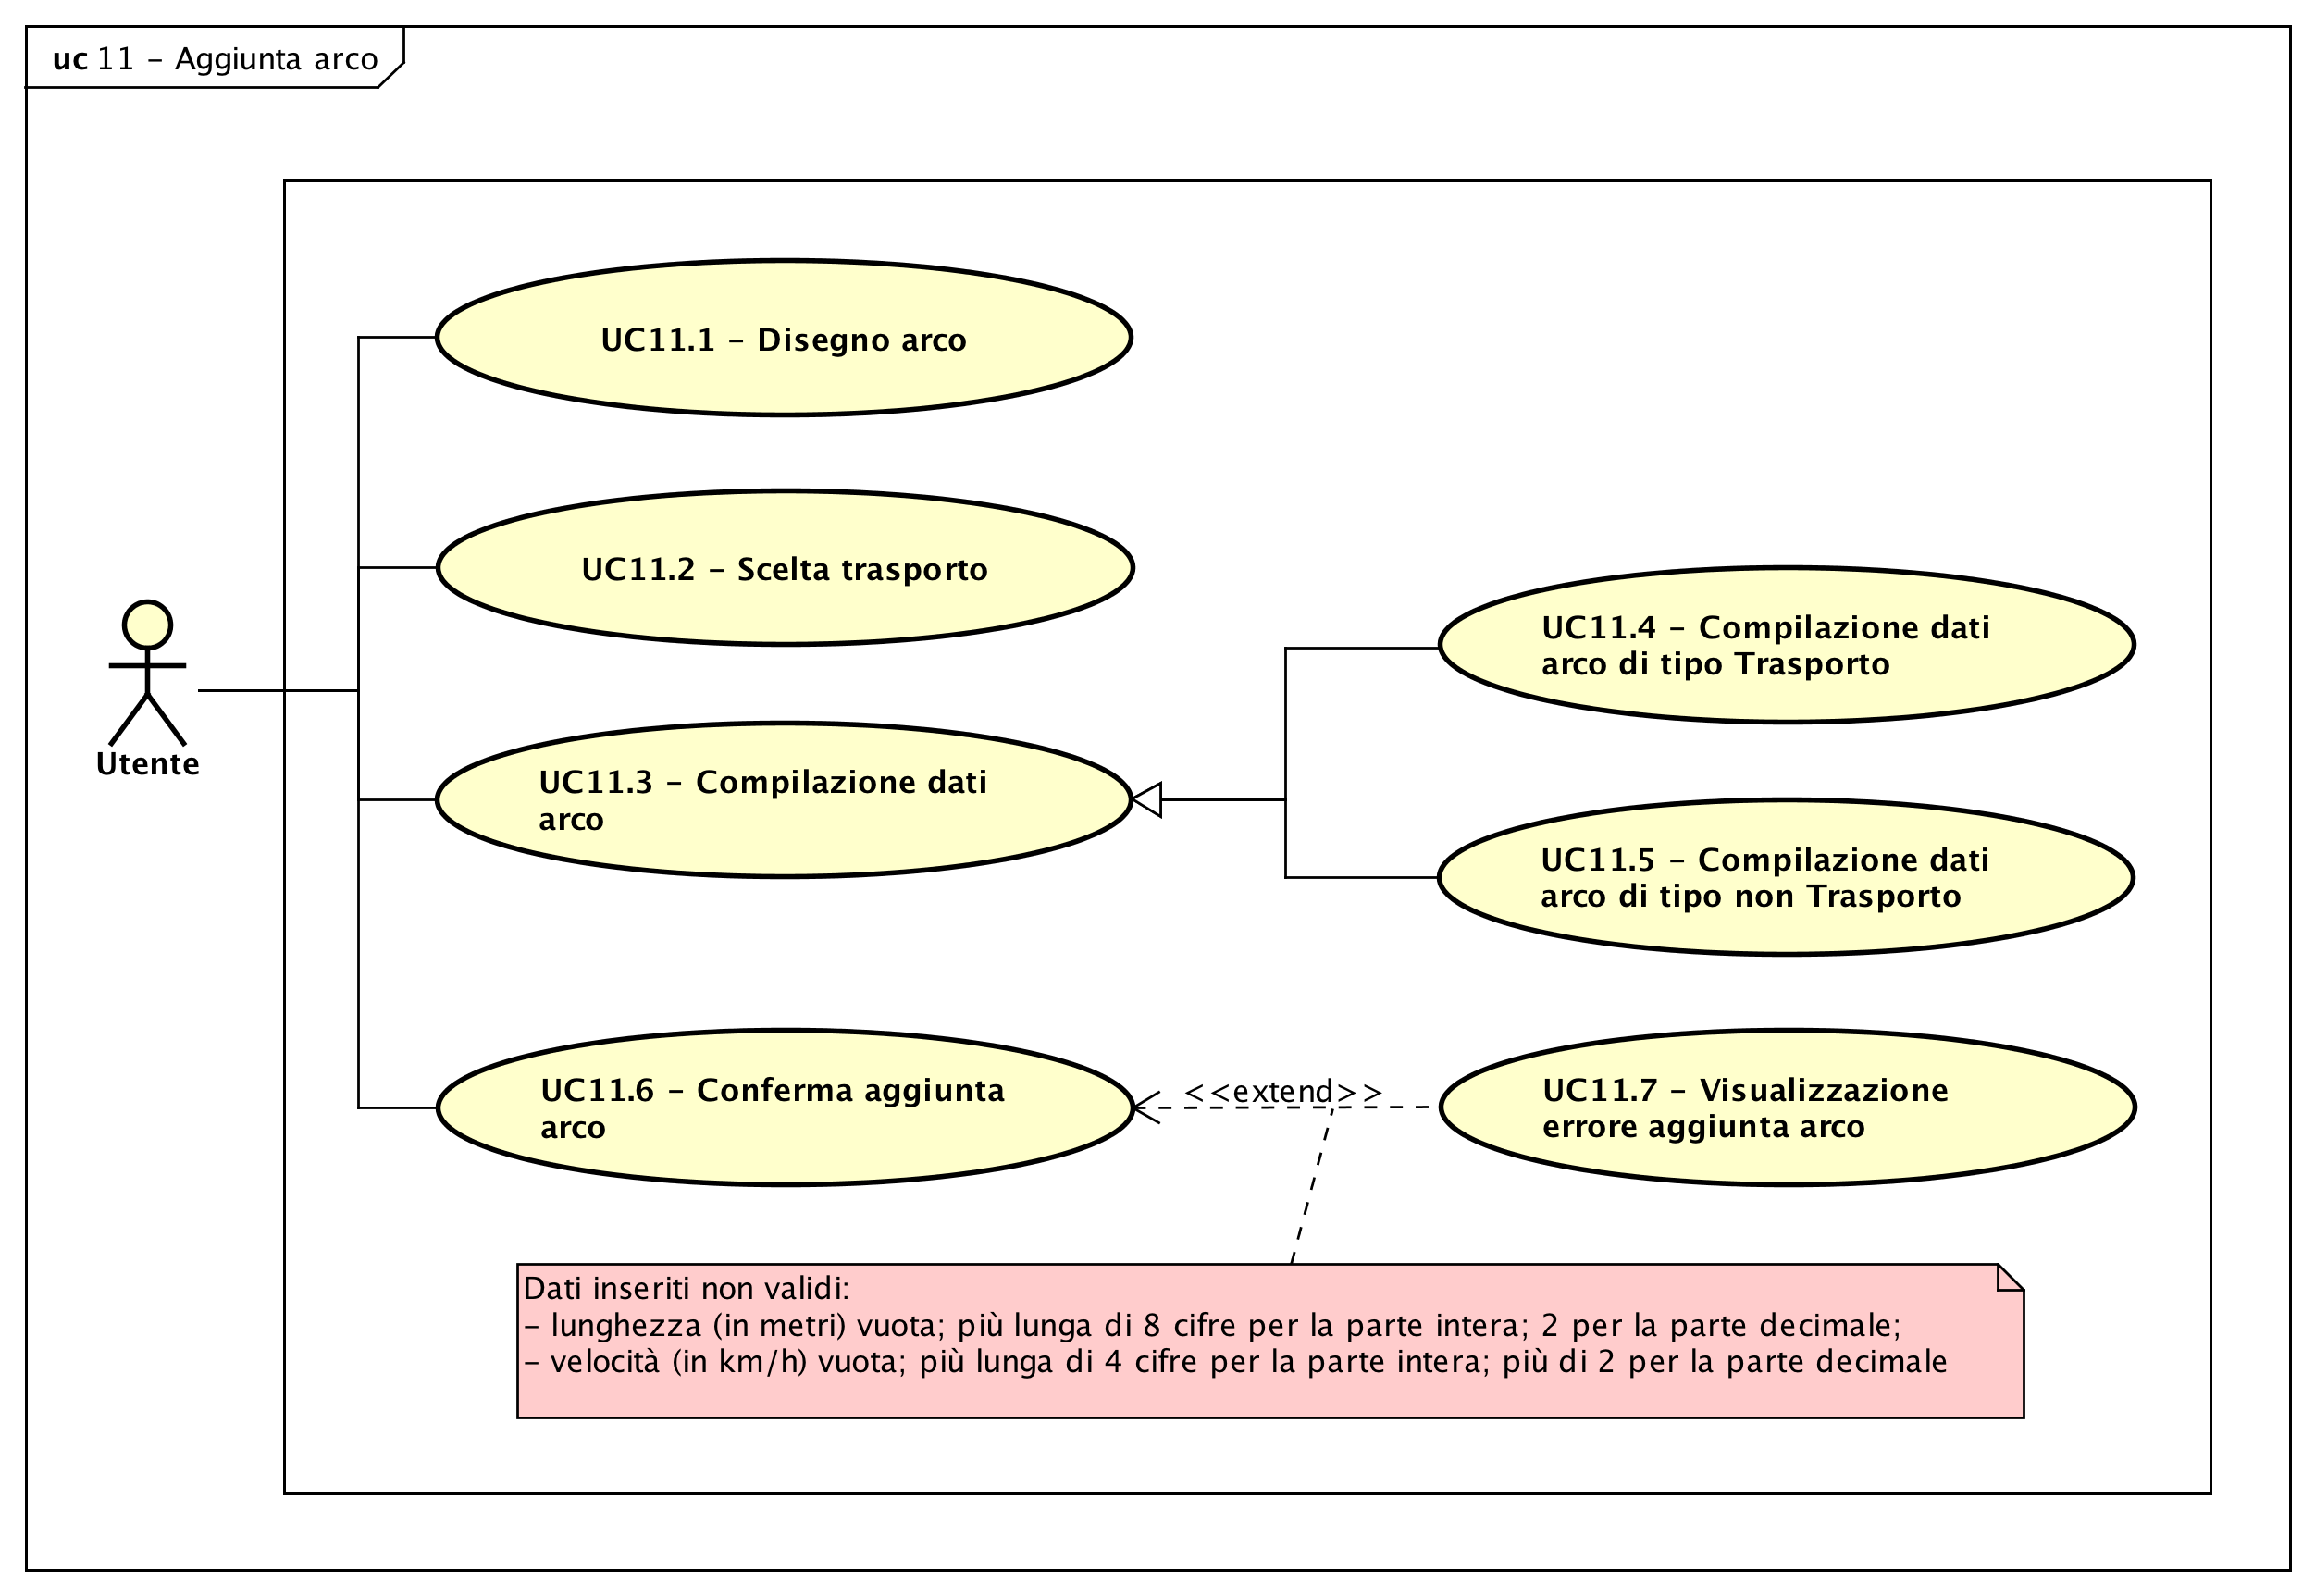
\includegraphics[width=\textwidth]{{img/uc11}.png} 
	\caption{UC11 - Aggiunta arco}
\end{figure}
\def\arraystretch{1.5}
\rowcolors{2}{D}{P}
\begin{tabularx}{\textwidth}{l|p{0.7\textwidth}}
	\rowcolor{I} \multicolumn{2}{c}{\color{white}\textbf{UC11 - Aggiunta arco}} \\
	\toprule
	\endhead
	\textbf{Attori} & Utente\\
	\textbf{Descrizione} & l'utente aggiunge un arco\\
	\textbf{Pre-condizione} & l'utente ha aperto l'applicazione; è stato inserito almeno un nodo\\
	\textbf{Post-condizione} & un nuovo arco è stato aggiunto ed è visualizzabile sulla mappa; l'utente visualizza un messaggio che comunica la corretta esecuzione dell'operazione; l'area informativa rimane impostata sull'arco appena inserito; la posizione e il livello di ingrandimento della mappa rimangono invariati\\
	\textbf{Scenario principale} & \vspace{-1.2em}\begin{enumerate}[leftmargin=*,noitemsep,nosep]
		\item \nameref{sssec:UC11.1};
		\item \nameref{sssec:UC11.2};
		\item \nameref{sssec:UC11.3};
		\item \nameref{sssec:UC11.4};
		\item \nameref{sssec:UC11.5};
		\item \nameref{sssec:UC11.6}.
	\end{enumerate}\\
	\textbf{Estensioni} & \vspace{-1.2em}\begin{itemize}[leftmargin=*,noitemsep,nosep]
		\item \nameref{sssec:UC36}: l'utente interrompe volontariamente l'aggiunta dell'arco
	\end{itemize}\\
	\textbf{Scenari alternativi} & \vspace{-1.2em}\begin{itemize}[leftmargin=*,noitemsep,nosep]
		\item \nameref{sssec:UC11.7}.
	\end{itemize}\\
	%\textbf{Generalizzazioni} &  \\
	\bottomrule
\end{tabularx}
\subsection{UC11.1 - Disegno arco} 
\label{sssec:UC11.1} 
\begin{figure}[H] 
	\centering 
	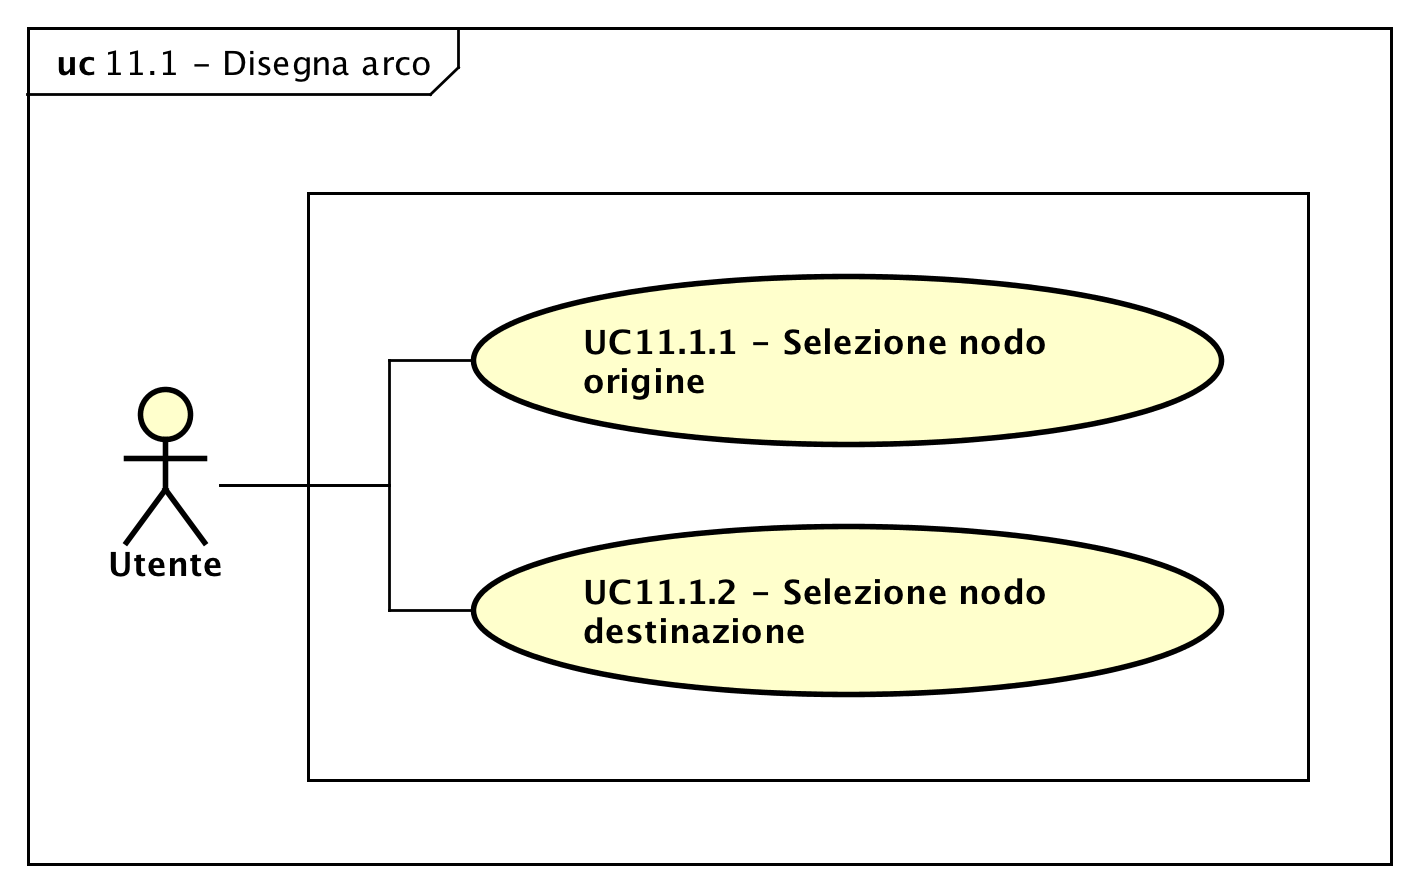
\includegraphics[scale=0.5]{{img/uc11.1}.png} 
	\caption{UC11.1 - Disegno arco}
\end{figure}
\def\arraystretch{1.5}
\rowcolors{2}{D}{P}
\begin{tabularx}{\textwidth}{l|p{0.7\textwidth}}
	\rowcolor{I} \multicolumn{2}{c}{\color{white}\textbf{UC11.1 - Disegno arco}} \\
	\toprule
	\endhead
	\textbf{Attori} & Utente\\
	\textbf{Descrizione} & l'utente disegna un arco\\
	\textbf{Pre-condizione} & esistono almeno due nodi all'interno del sistema\\
	\textbf{Post-condizione} & un arco che collega due nodi è stato disegnato ed è visualizzabile sulla mappa; l'utente può procedere a compilare gli altri dati dell'arco\\
	\textbf{Scenario principale} & \vspace{-1.2em}\begin{enumerate}[leftmargin=*,noitemsep,nosep]
		\item \nameref{sssec:UC11.1.1};
		\item \nameref{sssec:UC11.1.2}.
	\end{enumerate}\\
	%\textbf{Generalizzazioni} &  \\
	\bottomrule
\end{tabularx}
\subsection{UC11.1.1 - Selezione nodo di origine} 
\label{sssec:UC11.1.1} 
\def\arraystretch{1.5}
\rowcolors{2}{D}{P}
\begin{tabularx}{\textwidth}{l|p{0.7\textwidth}}
	\rowcolor{I} \multicolumn{2}{c}{\color{white}\textbf{UC11.1.1 - Selezione nodo di origine}} \\
	\toprule
	\endhead
	\textbf{Attori} & Utente\\
	\textbf{Descrizione} & l'utente seleziona il nodo di origine dell'arco\\
	\textbf{Pre-condizione} & il sistema offre la possibilità di selezionare il nodo di origine\\
	\textbf{Post-condizione} & il nodo di origine è stato selezionato; l'utente può procedere a selezionare il nodo di destinazione\\
	\textbf{Scenario principale} & \vspace{-1.2em}\begin{enumerate}[leftmargin=*,noitemsep,nosep]
		\item \nameref{sssec:UC11.1.1}.
	\end{enumerate}\\
	%\textbf{Generalizzazioni} &  \\
	\bottomrule
\end{tabularx}
\subsection{UC11.1.2 - Selezione nodo di destinazione} 
\label{sssec:UC11.1.2} 
\def\arraystretch{1.5}
\rowcolors{2}{D}{P}
\begin{tabularx}{\textwidth}{l|p{0.7\textwidth}}
	\rowcolor{I} \multicolumn{2}{c}{\color{white}\textbf{UC11.1.2 - Selezione nodo di destinazione}} \\
	\toprule
	\endhead
	\textbf{Attori} & Utente\\
	\textbf{Descrizione} & l'utente seleziona il nodo di destinazione dell'arco\\
	\textbf{Pre-condizione} & il sistema offre la possibilità di selezionare il nodo di destinazione\\
	\textbf{Post-condizione} & il nodo di destinazione è stato selezionato; un arco che collega due nodi è stato disegnato ed è visualizzabile sulla mappa; l'utente può procedere a compilare gli altri dati dell'arco\\
	\textbf{Scenario principale} & \vspace{-1.2em}\begin{enumerate}[leftmargin=*,noitemsep,nosep]
		\item \nameref{sssec:UC11.1.2}.
	\end{enumerate}\\
	%\textbf{Generalizzazioni} &  \\
	\bottomrule
\end{tabularx}
\subsection{UC11.2 - Scelta trasporto} 
\label{sssec:UC11.2} 
\def\arraystretch{1.5}
\rowcolors{2}{D}{P}
\begin{tabularx}{\textwidth}{l|p{0.7\textwidth}}
	\rowcolor{I} \multicolumn{2}{c}{\color{white}\textbf{UC11.2 - Scelta trasporto}} \\
	\toprule
	\endhead
	\textbf{Attori} & Utente\\
	\textbf{Descrizione} & l'utente sceglie se l'arco è di tipo trasporto oppure no\\
	\textbf{Pre-condizione} & il sistema offre la possibilità di specificare se un arco è di tipo trasporto\\
	\textbf{Post-condizione} & l'utente ha scelto se l'arco è di tipo trasporto oppure no; se è di tipo trasporto può visualizzare i dati da compilare relativi all'arco nell'area informativa\\
	\textbf{Scenario principale} & \vspace{-1.2em}\begin{enumerate}[leftmargin=*,noitemsep,nosep]
		\item \nameref{sssec:UC11.2}.
	\end{enumerate}\\
	%\textbf{Generalizzazioni} &  \\
	\bottomrule
\end{tabularx}
\subsection{UC11.3 - Compilazione dati arco} 
\label{sssec:UC11.3} 
\def\arraystretch{1.5}
\rowcolors{2}{D}{P}
\begin{tabularx}{\textwidth}{l|p{0.7\textwidth}}
	\rowcolor{I} \multicolumn{2}{c}{\color{white}\textbf{UC11.3 - Compilazione dati arco}} \\
	\toprule
	\endhead
	\textbf{Attori} & Utente\\
	\textbf{Descrizione} & l'utente compila i dati dell'arco\\
	\textbf{Pre-condizione} & il sistema offre la possibilità di compilare i dati dell'arco\\
	\textbf{Post-condizione} & i dati dell'arco sono stati compilati; l'utente viene riportato alla schermata di aggiunta dell'arco, dove può confermare l'aggiunta\\
		\textbf{Generalizzazioni} &
	\vspace{-1.2em}\begin{enumerate}
		[leftmargin=*,noitemsep,nosep]
		\item \nameref{sssec:UC11.4};
		\item \nameref{sssec:UC11.5}.
	\end{enumerate} \\
	\textbf{Generalizzazioni} &
	\vspace{-1.2em}\begin{itemize}
		[leftmargin=*,noitemsep,nosep]
		\item \nameref{sssec:UC11.4};
		\item \nameref{sssec:UC11.5}.
	\end{itemize} \\
	\bottomrule
\end{tabularx}
\subsection{UC11.4 - Compilazione dati arco di tipo Trasporto} 
\label{sssec:UC11.4} 
\begin{figure}[H] 
	\centering 
	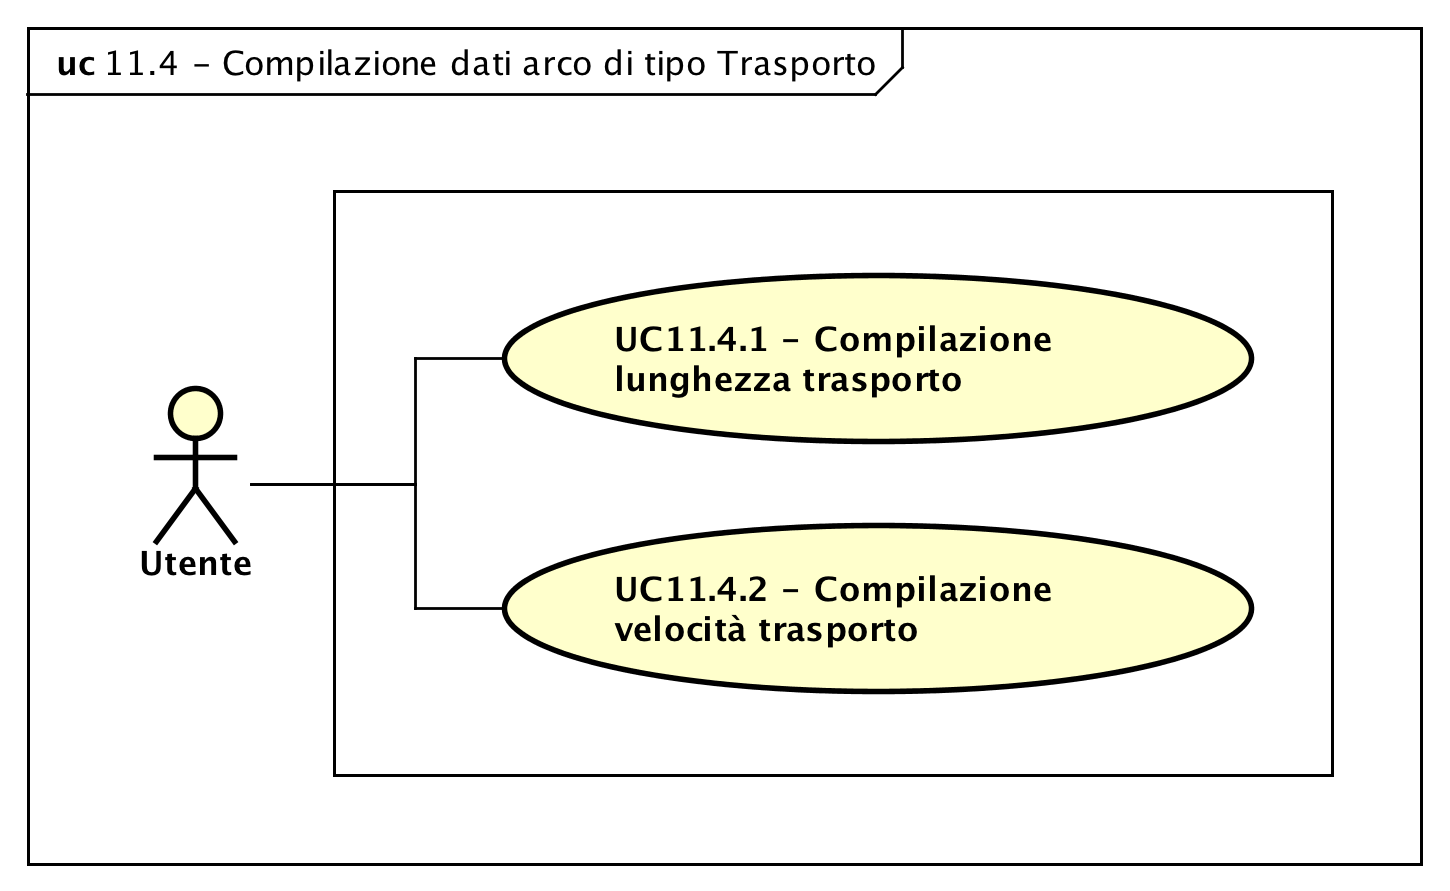
\includegraphics[scale=0.5]{{img/uc11.4}.png} 
	\caption{UC11.4 - Compilazione dati arco di tipo Trasporto}
\end{figure}
\def\arraystretch{1.5}
\rowcolors{2}{D}{P}
\begin{tabularx}{\textwidth}{l|p{0.7\textwidth}}
	\rowcolor{I} \multicolumn{2}{c}{\color{white}\textbf{UC11.4 - Compilazione dati arco di tipo Trasporto}} \\
	\toprule
	\endhead
	\textbf{Attori} & Utente\\
	\textbf{Descrizione} & l'utente compila i dati dell'arco di tipo Trasporto\\
	\textbf{Pre-condizione} & l'utente ha specificato che l'arco è di tipo Trasporto\\
	\textbf{Post-condizione} & i dati dell'arco di tipo Trasporto  sono stati compilati; l'utente viene riportato alla schermata di aggiunta dell'arco, dove può confermare l'aggiunta\\
	\textbf{Scenario principale} & \vspace{-1.2em}\begin{enumerate}[leftmargin=*,noitemsep,nosep]
		\item \nameref{sssec:UC11.4.1};
		\item \nameref{sssec:UC11.4.2}.
	\end{enumerate}\\
	%\textbf{Generalizzazioni} &  \\
	\bottomrule
\end{tabularx}
\subsection{UC11.4.1 - Compilazione lunghezza trasporto} 
\label{sssec:UC11.4.1} 
\def\arraystretch{1.5}
\rowcolors{2}{D}{P}
\begin{tabularx}{\textwidth}{l|p{0.7\textwidth}}
	\rowcolor{I} \multicolumn{2}{c}{\color{white}\textbf{UC11.4.1 - Compilazione lunghezza trasporto}} \\
	\toprule
	\endhead
	\textbf{Attori} & Utente\\
	\textbf{Descrizione} & l'utente compila il campo relativo alla lunghezza del trasporto\\
	\textbf{Pre-condizione} & il sistema offre la possibilità di compilare il campo relativo alla lunghezza del trasporto\\
	\textbf{Post-condizione} & il campo relativo alla lunghezza del trasporto è stato compilato; l'utente visualizza il campo appena compilato nell'area informativa\\
	\textbf{Scenario principale} & \vspace{-1.2em}\begin{enumerate}[leftmargin=*,noitemsep,nosep]
		\item \nameref{sssec:UC11.4.1}.
	\end{enumerate}\\
	%\textbf{Generalizzazioni} &  \\
	\bottomrule
\end{tabularx}
\subsection{UC11.4.2 - Compilazione velocità trasporto} 
\label{sssec:UC11.4.2} 
\def\arraystretch{1.5}
\rowcolors{2}{D}{P}
\begin{tabularx}{\textwidth}{l|p{0.7\textwidth}}
	\rowcolor{I} \multicolumn{2}{c}{\color{white}\textbf{UC11.4.2 - Compilazione velocità trasporto}} \\
	\toprule
	\endhead
	\textbf{Attori} & Utente\\
	\textbf{Descrizione} & l'utente compila il campo relativo alla velocità del trasporto\\
	\textbf{Pre-condizione} & il sistema offre la possibilità di compilare il campo relativo alla velocità del trasporto\\
	\textbf{Post-condizione} & il campo relativo alla lunghezza del trasporto è stato compilato; l'utente visualizza il campo appena compilato nell'area informativa\\
	\textbf{Scenario principale} & \vspace{-1.2em}\begin{enumerate}[leftmargin=*,noitemsep,nosep]
		\item \nameref{sssec:UC11.4.2}.
	\end{enumerate}\\
	%\textbf{Generalizzazioni} &  \\
	\bottomrule
\end{tabularx}
\subsection{UC11.5 - Compilazione dati arco di tipo non Trasporto} 
\label{sssec:UC11.5} 
\def\arraystretch{1.5}
\rowcolors{2}{D}{P}
\begin{tabularx}{\textwidth}{l|p{0.7\textwidth}}
	\rowcolor{I} \multicolumn{2}{c}{\color{white}\textbf{UC11.5 - Compilazione dati arco di tipo non Trasporto}} \\
	\toprule
	\endhead
	\textbf{Attori} & Utente\\
	\textbf{Descrizione} & l'utente compila i dati dell'arco di tipo non Trasporto\\
	\textbf{Pre-condizione} & l'utente ha disegnato l'arco; l'utente ha specificato che l'arco è di tipo non Trasporto\\
	\textbf{Post-condizione} & i dati dell'arco di tipo non Trasporto sono stati compilati; l'utente viene riportato alla schermata di aggiunta dell'arco, dove può confermare l'aggiunta\\
	\textbf{Scenario principale} & \vspace{-1.2em}\begin{enumerate}[leftmargin=*,noitemsep,nosep]
		\item \nameref{sssec:UC11.5}.
	\end{enumerate}\\
	%\textbf{Generalizzazioni} &  \\
	\bottomrule
\end{tabularx}
\subsection{UC11.6 - Conferma aggiunta arco} 
\label{sssec:UC11.6} 
\def\arraystretch{1.5}
\rowcolors{2}{D}{P}
\begin{tabularx}{\textwidth}{l|p{0.7\textwidth}}
	\rowcolor{I} \multicolumn{2}{c}{\color{white}\textbf{UC11.6 - Conferma aggiunta arco}} \\
	\toprule
	\endhead
	\textbf{Attori} & Utente\\
	\textbf{Descrizione} & l'utente conferma l'aggiunta dell'arco\\
	\textbf{Pre-condizione} & il sistema offre la possibilità di confermare l'aggiunta dell'arco\\
	\textbf{Post-condizione} & un nuovo arco è stato aggiunto ed è visualizzabile sulla mappa; l'utente visualizza un messaggio che comunica la corretta esecuzione dell'operazione; l'area informativa rimane impostata sull'arco appena inserito; la posizione e il livello di ingrandimento della mappa rimangono invariati\\
	\textbf{Scenario principale} & \vspace{-1.2em}\begin{enumerate}[leftmargin=*,noitemsep,nosep]
		\item \nameref{sssec:UC11.6}.
	\end{enumerate}\\
	\textbf{Estensioni} & \vspace{-1.2em}\begin{itemize}[leftmargin=*,noitemsep,nosep]
		\item \nameref{sssec:UC11.7}: dati inseriti non validi:
		\begin{itemize}
			\item lunghezza (in metri) vuota;
			più lunga di 8 cifre per la parte intera; 2 per la parte
			decimale;
			\item velocità (in km/h) vuota; più
			lunga di 4 cifre per la parte intera; più di 2 per la parte
			decimale.
		\end{itemize} 
	\end{itemize}\\
	%\textbf{Generalizzazioni} &  \\
	\bottomrule
\end{tabularx}
\subsection{UC11.7 - Visualizzazione errore aggiunta arco} 
\label{sssec:UC11.7} 
\def\arraystretch{1.5}
\rowcolors{2}{D}{P}
\begin{tabularx}{\textwidth}{l|p{0.7\textwidth}}
	\rowcolor{I} \multicolumn{2}{c}{\color{white}\textbf{UC11.7 - Visualizzazione errore aggiunta arco}} \\
	\toprule
	\endhead
	\textbf{Attori} & Utente\\
	\textbf{Descrizione} & l'utente visualizza un errore relativo ai dati dell'arco compilati in modo errato\\
	\textbf{Pre-condizione} & l'utente sta tentando di inserire un nuovo arco\\
	\textbf{Post-condizione} & nessun nuovo arco inserito; l'utente visualizza un errore relativo ai dati dell'arco compilati in modo errato; l'utente viene riportato alla schermata di aggiunta arco\\
	\textbf{Scenario principale} & \vspace{-1.2em}\begin{enumerate}[leftmargin=*,noitemsep,nosep]
		\item \nameref{sssec:UC11.7}.
	\end{enumerate}\\
	%\textbf{Generalizzazioni} &  \\
	\bottomrule
\end{tabularx}
\subsection{UC12 - Visualizzazione info arco} 
\label{sssec:UC12} 
\def\arraystretch{1.5}
\rowcolors{2}{D}{P}
\begin{tabularx}{\textwidth}{l|p{0.7\textwidth}}
	\rowcolor{I} \multicolumn{2}{c}{\color{white}\textbf{UC12 - Visualizzazione info arco}} \\
	\toprule
	\endhead
	\textbf{Attori} & Utente\\
	\textbf{Descrizione} & l'utente seleziona un arco e ne visualizza le informazioni\\
	\textbf{Pre-condizione} & l'utente ha aperto l'applicazione, è stato inserito almeno un arco\\
	\textbf{Post-condizione} & il sistema mostra nell'area informativa le informazioni dell'arco selezionato; la posizione e il livello di ingrandimento della mappa rimangono invariati\\
	\textbf{Scenario principale} & \vspace{-1.2em}\begin{enumerate}[leftmargin=*,noitemsep,nosep]
		\item \nameref{sssec:UC12}.
	\end{enumerate}\\
	%\textbf{Generalizzazioni} &  \\
	\bottomrule
\end{tabularx}
\subsection{UC13 - Chiusura visualizzazione info arco} 
\label{sssec:UC13} 
\def\arraystretch{1.5}
\rowcolors{2}{D}{P}
\begin{tabularx}{\textwidth}{l|p{0.7\textwidth}}
	\rowcolor{I} \multicolumn{2}{c}{\color{white}\textbf{UC13 - Chiusura visualizzazione info arco}} \\
	\toprule
	\endhead
	\textbf{Attori} & Utente\\
	\textbf{Descrizione} & l'utente chiude la visualizzazione delle informazioni di un arco\\
	\textbf{Pre-condizione} & l'utente ha visualizzato le informazioni di un arco\\
	\textbf{Post-condizione} & è stata chiusa la visualizzazione delle informazioni dell'arco selezionato nell'area informativa; l'area informativa viene impostata sulla visualizzazione di default; la posizione e il livello di ingrandimento della mappa rimangono invariati\\
	\textbf{Scenario principale} & \vspace{-1.2em}\begin{enumerate}[leftmargin=*,noitemsep,nosep]
		\item \nameref{sssec:UC13}.
	\end{enumerate}\\
	%\textbf{Generalizzazioni} &  \\
	\bottomrule
\end{tabularx}
\subsection{UC14 - Modifica arco} 
\label{sssec:UC14} 
\begin{figure}[H] 
	\centering 
	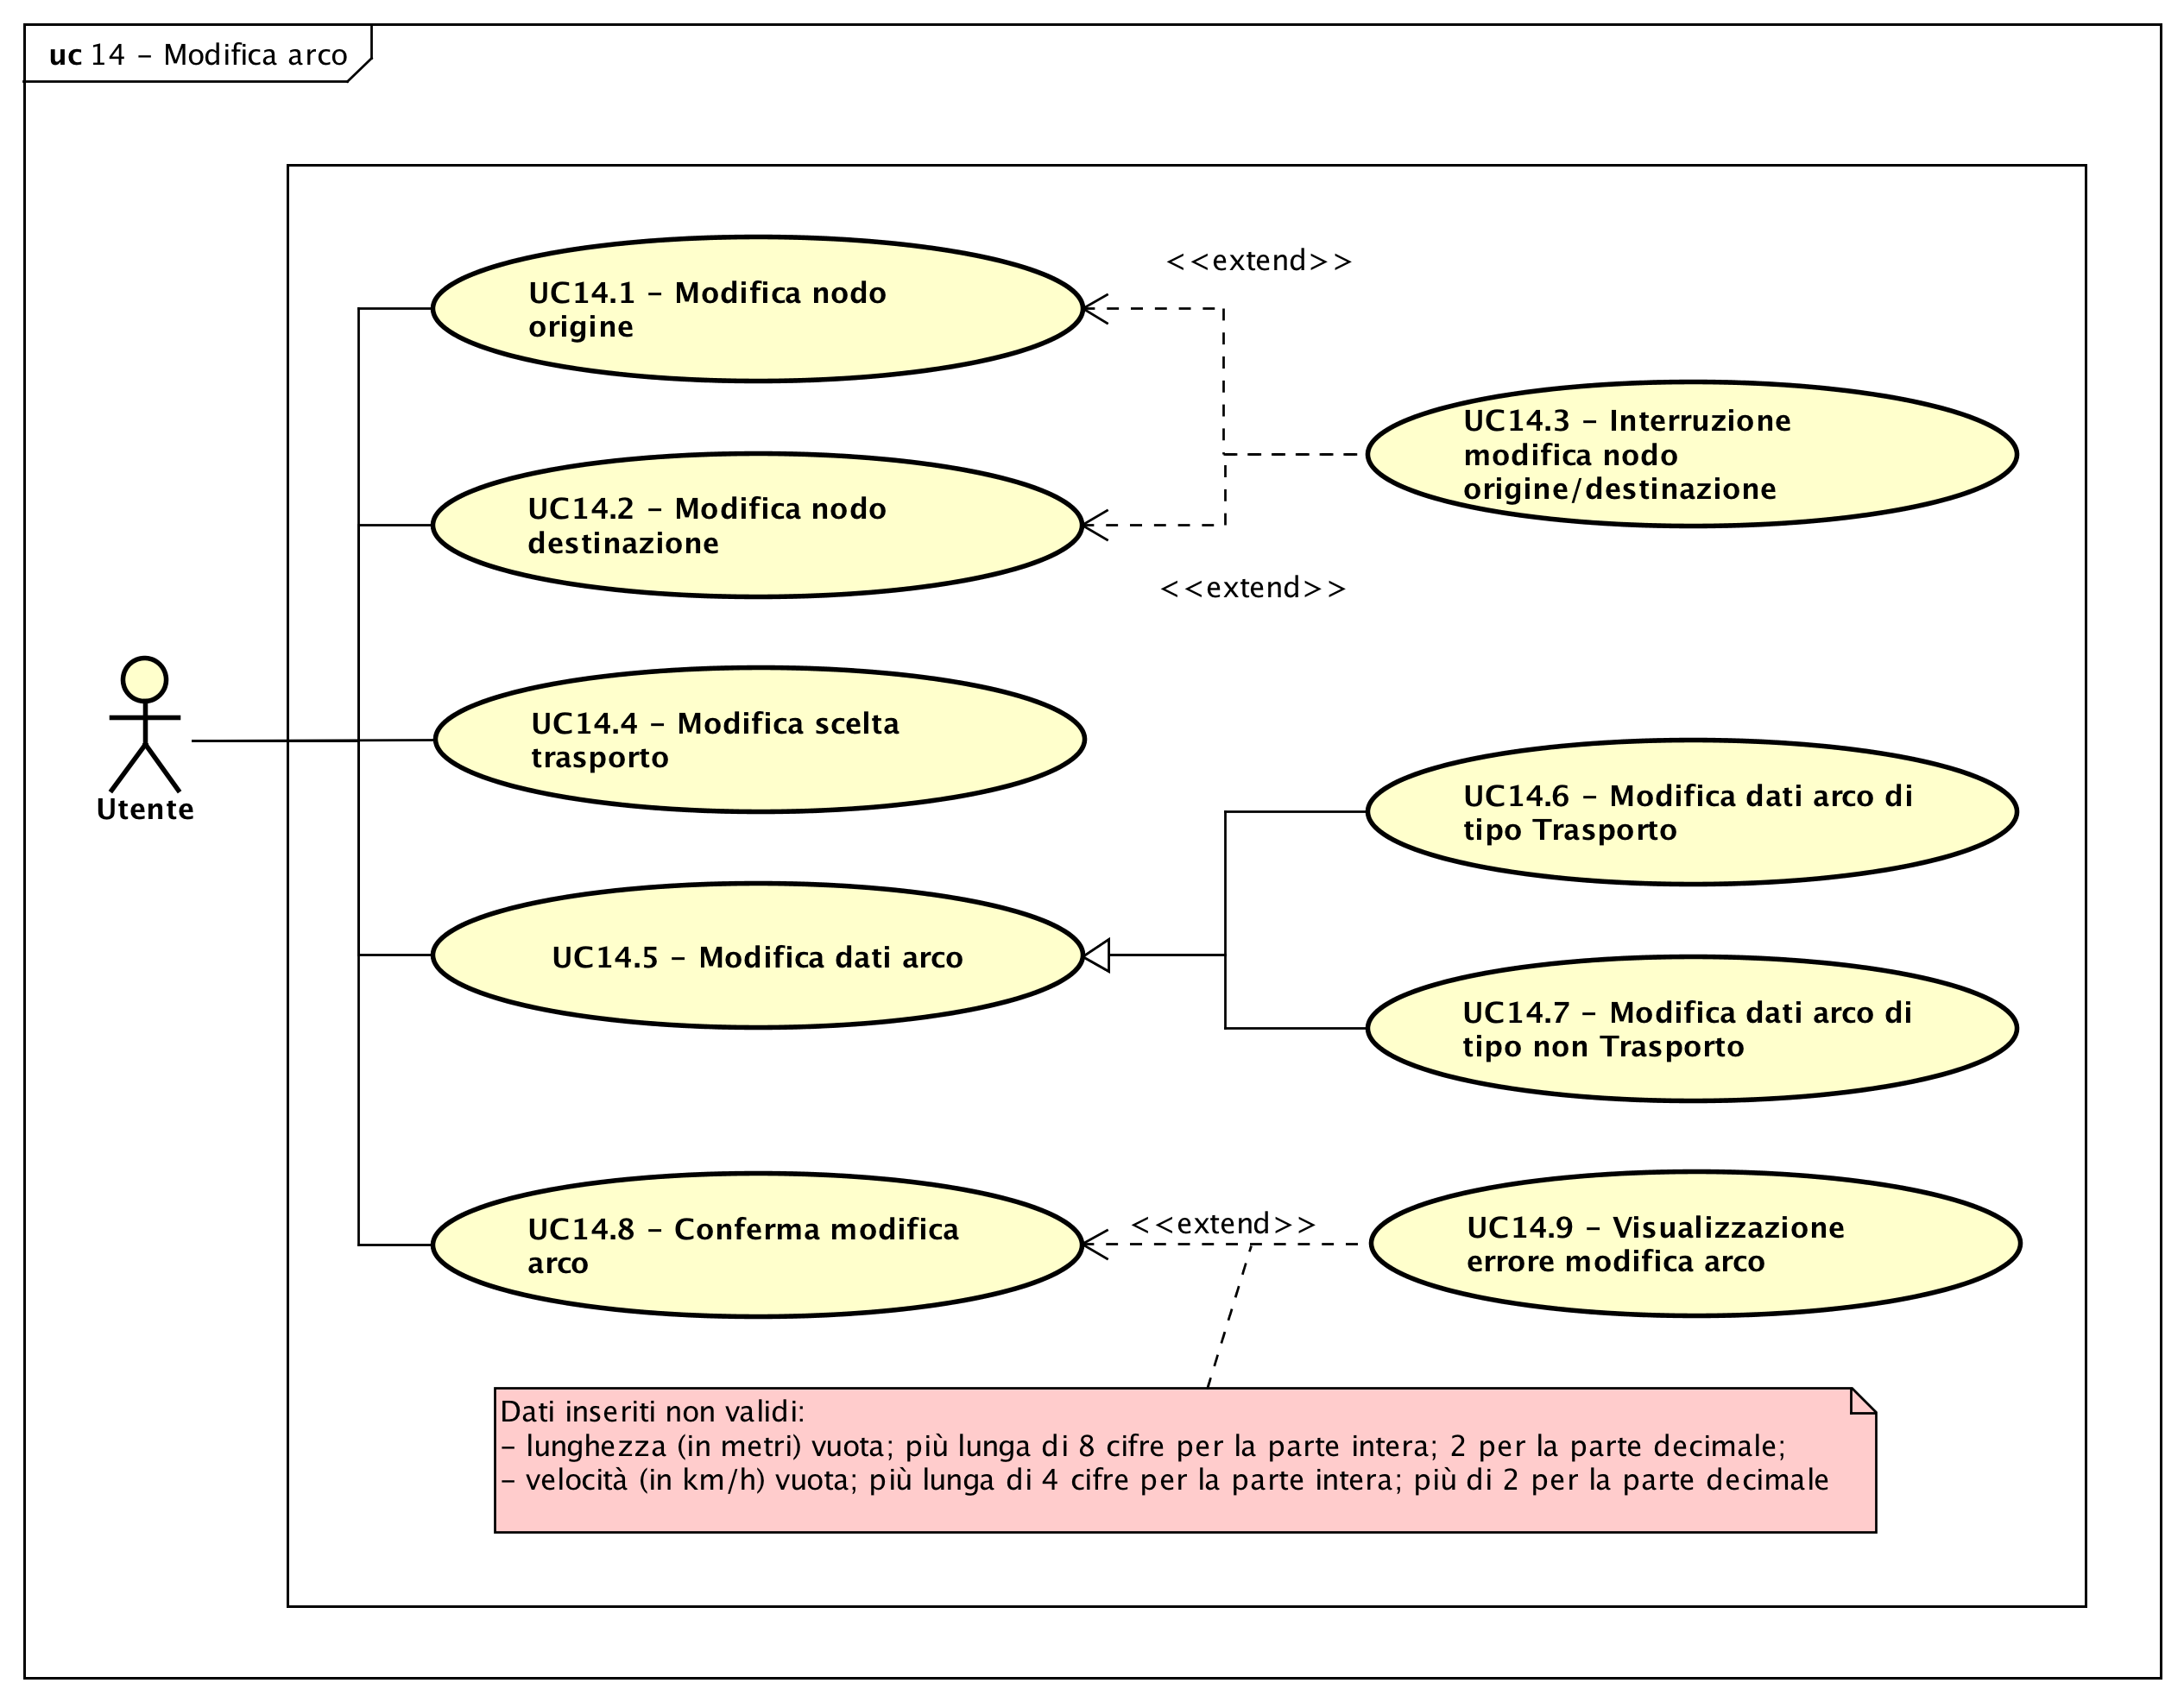
\includegraphics[width=\textwidth]{{img/uc14}.png} 
	\caption{UC14 - Modifica arco}
\end{figure}
\def\arraystretch{1.5}
\rowcolors{2}{D}{P}
\begin{tabularx}{\textwidth}{l|p{0.7\textwidth}}
	\rowcolor{I} \multicolumn{2}{c}{\color{white}\textbf{UC14 - Modifica arco}} \\
	\toprule
	\endhead
	\textbf{Attori} & Utente\\
	\textbf{Descrizione} & l'utente modifica l'arco\\
	\textbf{Pre-condizione} & l'utente ha aperto l'applicazione; almeno un arco è stato aggiunto; l'utente ha selezionato un arco\\
	\textbf{Post-condizione} & l'arco è stato modificato; l'utente visualizza un messaggio che comunica la corretta esecuzione dell'operazione; l'area informativa rimane impostata sull'arco appena modificato; la posizione e il livello di ingrandimento della mappa rimangono invariati\\
	\textbf{Scenario principale} & \vspace{-1.2em}\begin{enumerate}[leftmargin=*,noitemsep,nosep]
		\item \nameref{sssec:UC14.1};
		\item \nameref{sssec:UC14.2};
		\item \nameref{sssec:UC14.4};
		\item \nameref{sssec:UC14.5};
		\item \nameref{sssec:UC14.6};
		\item \nameref{sssec:UC14.7};
		\item \nameref{sssec:UC14.8}.
	\end{enumerate}\\
	\textbf{Estensioni} & \vspace{-1.2em}\begin{itemize}[leftmargin=*,noitemsep,nosep]
		\item \nameref{sssec:UC37}: l'utente interrompe volontariamente la modifica dei dati
		dell'arco;
	\end{itemize}\\
	\textbf{Scenari alternativi} & \vspace{-1.2em}\begin{itemize}[leftmargin=*,noitemsep,nosep]
		\item \nameref{sssec:UC14.3};
		\item \nameref{sssec:UC14.9}.
	\end{itemize}\\
	%\textbf{Generalizzazioni} &  \\
	\bottomrule
\end{tabularx}
\subsection{UC14.1 - Modifica nodo origine} 
\label{sssec:UC14.1} 
\def\arraystretch{1.5}
\rowcolors{2}{D}{P}
\begin{tabularx}{\textwidth}{l|p{0.7\textwidth}}
	\rowcolor{I} \multicolumn{2}{c}{\color{white}\textbf{UC14.1 - Modifica nodo origine}} \\
	\toprule
	\endhead
	\textbf{Attori} & Utente\\
	\textbf{Descrizione} & l'utente modifica il nodo di origine dell'arco\\
	\textbf{Pre-condizione} & il sistema offre la possibilità di modificare il nodo di origine\\
	\textbf{Post-condizione} & il nodo di origine è stato modificato; l'arco parte dal nuovo nodo di origine indicato; l'utente viene riportato alla schermata di modifica arco\\
	\textbf{Scenario principale} & \vspace{-1.2em}\begin{enumerate}[leftmargin=*,noitemsep,nosep]
		\item \nameref{sssec:UC14.1}.
	\end{enumerate}\\
	\textbf{Estensioni} & \vspace{-1.2em}\begin{itemize}[leftmargin=*,noitemsep,nosep]
		\item \nameref{sssec:UC14.3}: l'utente interrompe volontariamente la modifica del nodo di
		origine/destinazione dell'arco
	\end{itemize}\\
	%\textbf{Generalizzazioni} &  \\
	\bottomrule
\end{tabularx}
\subsection{UC14.2 - Modifica nodo destinazione} 
\label{sssec:UC14.2} 
\def\arraystretch{1.5}
\rowcolors{2}{D}{P}
\begin{tabularx}{\textwidth}{l|p{0.7\textwidth}}
	\rowcolor{I} \multicolumn{2}{c}{\color{white}\textbf{UC14.2 - Modifica nodo destinazione}} \\
	\toprule
	\endhead
	\textbf{Attori} & Utente\\
	\textbf{Descrizione} & l'utente modifica il nodo di destinazione dell'arco\\
	\textbf{Pre-condizione} & il sistema offre la possibilità di modificare il nodo di destinazione\\
	\textbf{Post-condizione} & il nodo di destinazione è stato modificato; l'arco arriva nel nuovo nodo di destinazione indicato; l'utente viene riportato alla schermata di modifica arco\\
	\textbf{Scenario principale} & \vspace{-1.2em}\begin{enumerate}[leftmargin=*,noitemsep,nosep]
		\item \nameref{sssec:UC14.2}.
	\end{enumerate}\\
	\textbf{Estensioni} & \vspace{-1.2em}\begin{itemize}[leftmargin=*,noitemsep,nosep]
		\item \nameref{sssec:UC14.3}: l'utente interrompe volontariamente la modifica del nodo di
		origine/destinazione dell'arco;
	\end{itemize}\\
	%\textbf{Generalizzazioni} &  \\
	\bottomrule
\end{tabularx}
\subsection{UC14.3 - Interruzione modifica nodo origine/destinazione} 
\label{sssec:UC14.3} 
\def\arraystretch{1.5}
\rowcolors{2}{D}{P}
\begin{tabularx}{\textwidth}{l|p{0.7\textwidth}}
	\rowcolor{I} \multicolumn{2}{c}{\color{white}\textbf{UC14.3 - Interruzione modifica nodo origine/destinazione}} \\
	\toprule
	\endhead
	\textbf{Attori} & Utente\\
	\textbf{Descrizione} & l'utente interrompe la modifica del nodo di origine o di destinazione\\
	\textbf{Pre-condizione} & il sistema offre la possibilità di modificare il nodo di origine o di destinazione\\
	\textbf{Post-condizione} & il nodo di origine o di destinazione non è stato modificato; l'utente viene riportato alla schermata di modifica arco\\
	\textbf{Scenario principale} & \vspace{-1.2em}\begin{enumerate}[leftmargin=*,noitemsep,nosep]
		\item \nameref{sssec:UC14.3}
	\end{enumerate}\\
	%\textbf{Generalizzazioni} &  \\
	\bottomrule
\end{tabularx}
\subsection{UC14.4 - Modifica scelta trasporto} 
\label{sssec:UC14.4} 
\def\arraystretch{1.5}
\rowcolors{2}{D}{P}
\begin{tabularx}{\textwidth}{l|p{0.7\textwidth}}
	\rowcolor{I} \multicolumn{2}{c}{\color{white}\textbf{UC14.4 - Modifica scelta trasporto}} \\
	\toprule
	\endhead
	\textbf{Attori} & Utente\\
	\textbf{Descrizione} & l'utente modifica la scelta riguardo il trasporto\\
	\textbf{Pre-condizione} & il sistema offre la possibilità di modificare la scelta riguardo il trasporto\\
	\textbf{Post-condizione} & la scelta riguardo il trasporto è stata modificata; l'utente visualizza la nuova scelta nell'area informativa\\
	\textbf{Scenario principale} & \vspace{-1.2em}\begin{enumerate}[leftmargin=*,noitemsep,nosep]
		\item \nameref{sssec:UC14.4}.
	\end{enumerate}\\
	%\textbf{Generalizzazioni} &  \\
	\bottomrule
\end{tabularx}
\subsection{UC14.5 - Modifica dati arco} 
\label{sssec:UC14.5} 
\def\arraystretch{1.5}
\rowcolors{2}{D}{P}
\begin{tabularx}{\textwidth}{l|p{0.7\textwidth}}
	\rowcolor{I} \multicolumn{2}{c}{\color{white}\textbf{UC14.5 - Modifica dati arco}} \\
	\toprule
	\endhead
	\textbf{Attori} & Utente\\
	\textbf{Descrizione} & l'utente modifica i dati dell'arco\\
	\textbf{Pre-condizione} & l'utente ha specificato che l'arco è di tipo trasporto\\
	\textbf{Post-condizione} & l'utente ha modificato i dati dell'arco e li può visualizzare nell'area informativa; l'utente viene riportato alla schermata di modifica dell'arco\\
	\textbf{Generalizzazioni} &
	\vspace{-1.2em}\begin{enumerate}
		[leftmargin=*,noitemsep,nosep]
		\item \nameref{sssec:UC14.6};
		\item \nameref{sssec:UC14.7}.
	\end{enumerate} \\
\textbf{Generalizzazioni} &
\vspace{-1.2em}\begin{itemize}
	[leftmargin=*,noitemsep,nosep]
	\item \nameref{sssec:UC14.6};
	\item \nameref{sssec:UC14.7}.
\end{itemize} \\
	\bottomrule
\end{tabularx}


\subsection{UC14.6 - Modifica dati arco di tipo Trasporto} 
\label{sssec:UC14.6} 
\begin{figure}[H] 
	\centering 
	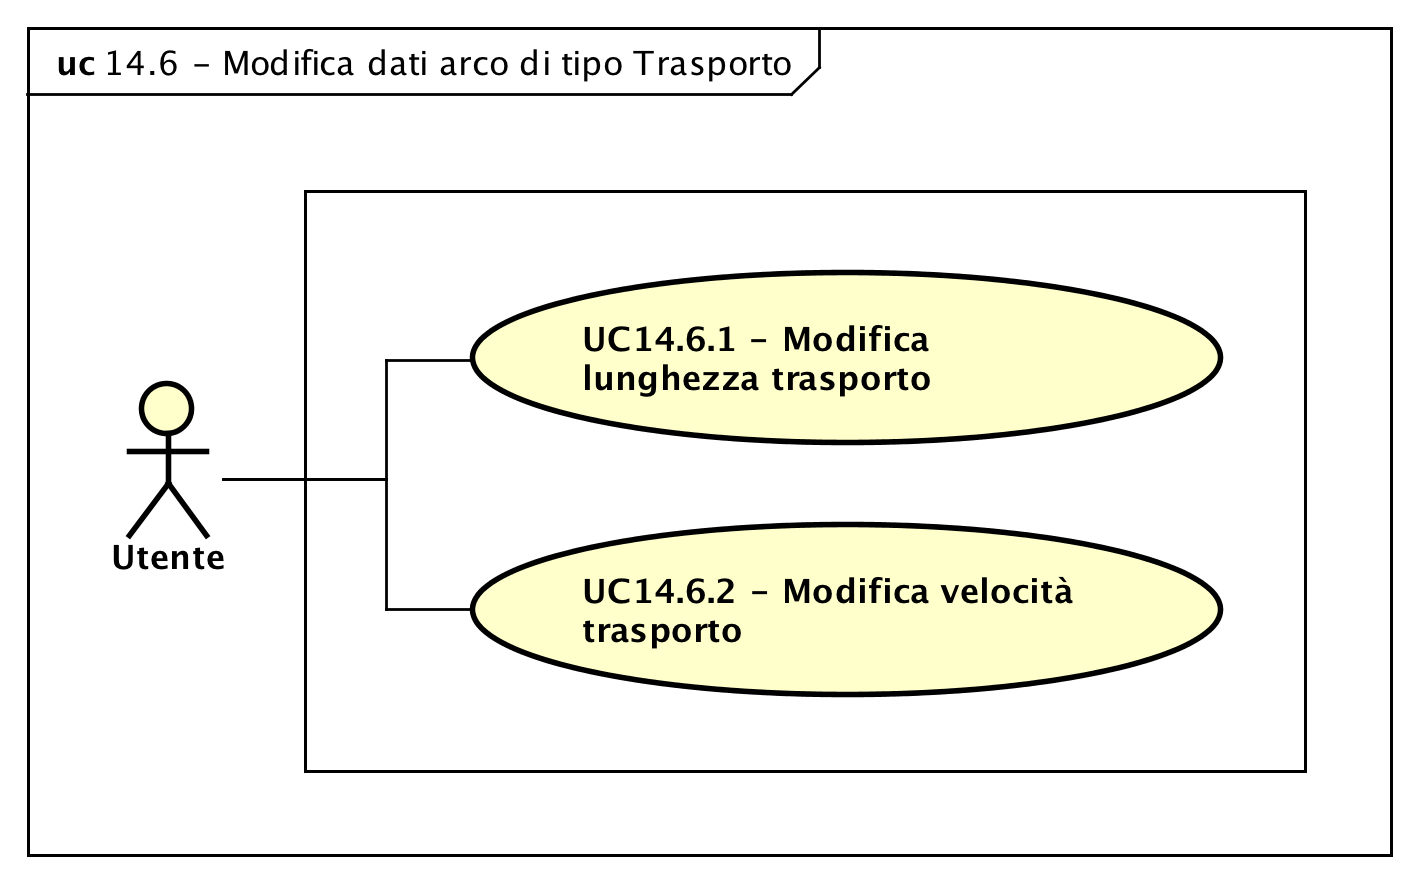
\includegraphics[scale=0.5]{{img/uc14.6}.png} 
	\caption{UC14.6 - Modifica dati arco di tipo Trasporto}
\end{figure}
\def\arraystretch{1.5}
\rowcolors{2}{D}{P}
\begin{tabularx}{\textwidth}{l|p{0.7\textwidth}}
	\rowcolor{I} \multicolumn{2}{c}{\color{white}\textbf{UC14.6 - Modifica dati arco di tipo Trasporto}} \\
	\toprule
	\endhead
	\textbf{Attori} & Utente\\
	\textbf{Descrizione} & l'utente modifica i dati dell'arco di tipo Trasporto\\
	\textbf{Pre-condizione} & l'utente ha specificato che l'arco è di tipo Trasporto\\
	\textbf{Post-condizione} & l'utente ha modificato i dati dell'arco di tipo Trasporto e li può visualizzare nell'area informativa; l'utente viene riportato alla schermata di modifica dell'arco\\
	\textbf{Scenario principale} & \vspace{-1.2em}\begin{enumerate}[leftmargin=*,noitemsep,nosep]
		\item \nameref{sssec:UC14.6.1};
		\item \nameref{sssec:UC14.6.2}.
	\end{enumerate}\\
	%\textbf{Generalizzazioni} &  \\
	\bottomrule
\end{tabularx}
\subsection{UC14.6.1 - Modifica lunghezza trasporto} 
\label{sssec:UC14.6.1} 
\def\arraystretch{1.5}
\rowcolors{2}{D}{P}
\begin{tabularx}{\textwidth}{l|p{0.7\textwidth}}
	\rowcolor{I} \multicolumn{2}{c}{\color{white}\textbf{UC14.6.1 - Modifica lunghezza trasporto}} \\
	\toprule
	\endhead
	\textbf{Attori} & Utente\\
	\textbf{Descrizione} & l'utente modifica la lunghezza del trasporto\\
	\textbf{Pre-condizione} & il sistema offre la possibilità di modificare la lunghezza del trasporto; l'utente ha specificato che il nodo è di tipo trasporto\\
	\textbf{Post-condizione} & la lunghezza del trasporto è stata modificata; l'utente visualizza la lunghezza appena inserita nell'area informativa\\
	\textbf{Scenario principale} & \vspace{-1.2em}\begin{enumerate}[leftmargin=*,noitemsep,nosep]
		\item \nameref{sssec:UC14.6.1}.
	\end{enumerate}\\
	%\textbf{Generalizzazioni} &  \\
	\bottomrule
\end{tabularx}
\subsection{UC14.6.2 - Modifica velocità trasporto} 
\label{sssec:UC14.6.2} 
\def\arraystretch{1.5}
\rowcolors{2}{D}{P}
\begin{tabularx}{\textwidth}{l|p{0.7\textwidth}}
	\rowcolor{I} \multicolumn{2}{c}{\color{white}\textbf{UC14.6.2 - Modifica velocità trasporto}} \\
	\toprule
	\endhead
	\textbf{Attori} & Utente\\
	\textbf{Descrizione} & l'utente modifica la velocità del trasporto\\
	\textbf{Pre-condizione} & il sistema offre la possibilità di modificare la velocità del trasporto; l'utente ha specificato che il nodo è di tipo trasporto\\
	\textbf{Post-condizione} & la velocità del trasporto è stata modificata; l'utente visualizza la nuova velocità appena inserita nell'area informativa\\
	\textbf{Scenario principale} & \vspace{-1.2em}\begin{enumerate}[leftmargin=*,noitemsep,nosep]
		\item \nameref{sssec:UC14.6.2}.
	\end{enumerate}\\
	%\textbf{Generalizzazioni} &  \\
	\bottomrule
\end{tabularx}
\subsection{UC14.7 - Modifica dati arco di tipo non Trasporto} 
\label{sssec:UC14.7} 
\def\arraystretch{1.5}
\rowcolors{2}{D}{P}
\begin{tabularx}{\textwidth}{l|p{0.7\textwidth}}
	\rowcolor{I} \multicolumn{2}{c}{\color{white}\textbf{UC14.7 - Modifica dati arco di tipo non Trasporto}} \\
	\toprule
	\endhead
	\textbf{Attori} & Utente\\
	\textbf{Descrizione} & l'utente modifica i dati dell'arco di tipo non Trasporto\\
	\textbf{Pre-condizione} & l'utente ha specificato che l'arco è di tipo non Trasporto\\
	\textbf{Post-condizione} & l'utente ha modificato i dati dell'arco di tipo non Trasporto e li può visualizzare nell'area informativa; l'utente viene riportato alla schermata di modifica dell'arco\\
	\textbf{Scenario principale} & \vspace{-1.2em}\begin{enumerate}[leftmargin=*,noitemsep,nosep]
		\item \nameref{sssec:UC14.7}.
	\end{enumerate}\\
	%\textbf{Generalizzazioni} &  \\
	\bottomrule
\end{tabularx}
\subsection{UC14.8 - Conferma modifica arco} 
\label{sssec:UC14.8} 
\def\arraystretch{1.5}
\rowcolors{2}{D}{P}
\begin{tabularx}{\textwidth}{l|p{0.7\textwidth}}
	\rowcolor{I} \multicolumn{2}{c}{\color{white}\textbf{UC14.8 - Conferma modifica arco}} \\
	\toprule
	\endhead
	\textbf{Attori} & Utente\\
	\textbf{Descrizione} & l'utente conferma la modifica dell'arco\\
	\textbf{Pre-condizione} & il sistema offre la possibilità di confermare la modifica dell'arco\\
	\textbf{Post-condizione} & l'arco è stato modificato;  l'utente visualizza un messaggio che comunica la corretta esecuzione dell'operazione; l'area informativa rimane impostata sull'arco appena modificato; la posizione e il livello di ingrandimento della mappa rimangono invariati\\
	\textbf{Scenario principale} & \vspace{-1.2em}\begin{enumerate}[leftmargin=*,noitemsep,nosep]
		\item \nameref{sssec:UC14.8}.
	\end{enumerate}\\
	\textbf{Estensioni} & \vspace{-1.2em}\begin{itemize}[leftmargin=*,noitemsep,nosep]
		\item \nameref{sssec:UC14.9}: dati inseriti non validi:
		\begin{itemize}
			\item lunghezza (in metri) vuota;
			più lunga di 8 cifre per la parte intera; 2 per la parte
			decimale;
			\item velocità (in km/h) vuota; più
			lunga di 4 cifre per la parte intera; più di 2 per la parte
			decimale.
		\end{itemize}
	\end{itemize}\\
	%\textbf{Generalizzazioni} &  \\
	\bottomrule
\end{tabularx}
\subsection{UC14.9 - Visualizzazione errore modifica arco} 
\label{sssec:UC14.9} 
\def\arraystretch{1.5}
\rowcolors{2}{D}{P}
\begin{tabularx}{\textwidth}{l|p{0.7\textwidth}}
	\rowcolor{I} \multicolumn{2}{c}{\color{white}\textbf{UC14.9 - Visualizzazione errore modifica arco}} \\
	\toprule
	\endhead
	\textbf{Attori} & Utente\\
	\textbf{Descrizione} & l'utente visualizza un errore relativo alla modifica dell'arco\\
	\textbf{Pre-condizione} & l'utente ha confermato la modifica dell'arco\\
	\textbf{Post-condizione} & l'arco non è stato modificato; l'utente visualizza un errore relativo ai dati del nodo compilati in modo errato; l'utente viene riportato alla schermata di modifica nodo\\
	\textbf{Scenario principale} & \vspace{-1.2em}\begin{enumerate}[leftmargin=*,noitemsep,nosep]
		\item \nameref{sssec:UC14.9}.
	\end{enumerate}\\
	%\textbf{Generalizzazioni} &  \\
	\bottomrule
\end{tabularx}
\subsection{UC15 - Eliminazione arco} 
\label{sssec:UC15} 
\begin{figure}[H] 
	\centering 
	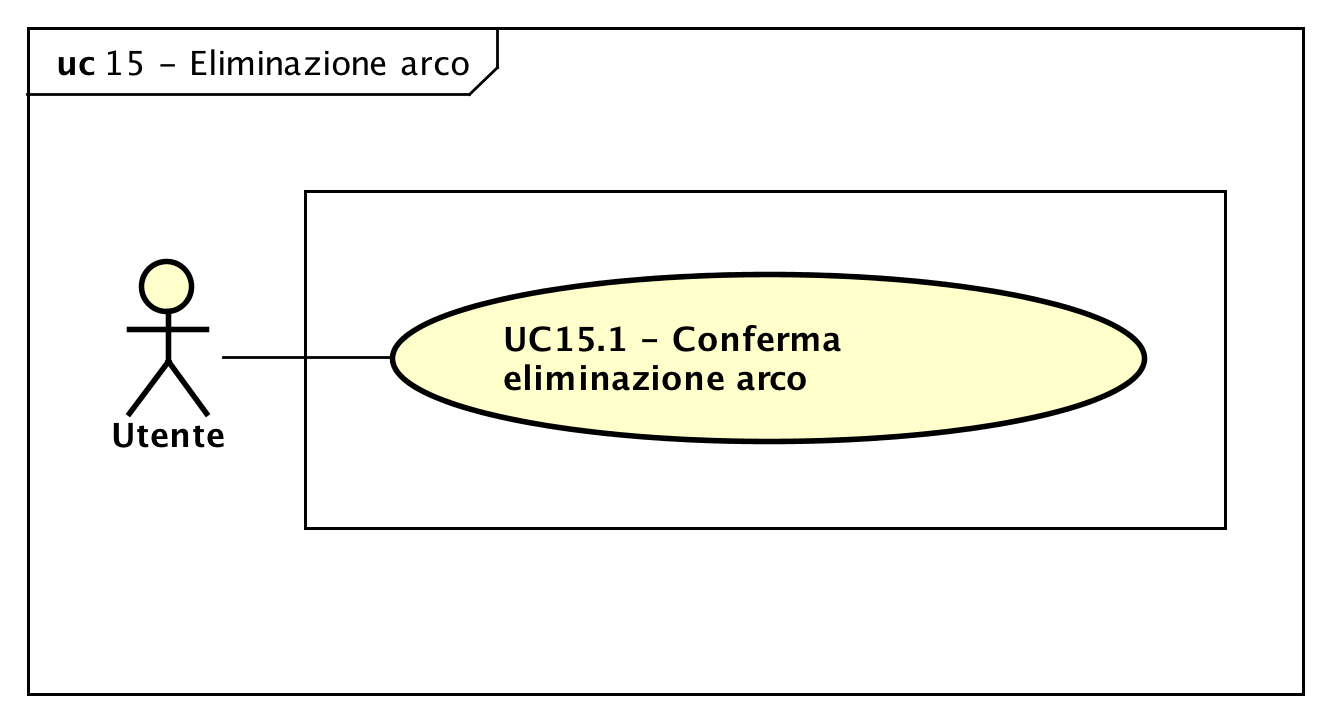
\includegraphics[scale=0.5]{{img/uc15}.png} 
	\caption{UC15 - Eliminazione arco}
\end{figure}
\def\arraystretch{1.5}
\rowcolors{2}{D}{P}
\begin{tabularx}{\textwidth}{l|p{0.7\textwidth}}
	\rowcolor{I} \multicolumn{2}{c}{\color{white}\textbf{UC15 - Eliminazione arco}} \\
	\toprule
	\endhead
	\textbf{Attori} & Utente\\
	\textbf{Descrizione} & l'utente elimina un arco\\
	\textbf{Pre-condizione} & l'utente ha aperto l'applicazione; è stato inserito almeno un arco; l'utente ha selezionato un arco\\
	\textbf{Post-condizione} & l'arco è stato eliminato e non è più visualizzato sulla mappa; l'utente visualizza un messaggio che comunica la corretta esecuzione dell'operazione; l'area informativa viene impostata sulla visualizzazione di default;  la posizione e il livello di ingrandimento della mappa rimangono invariati\\
	\textbf{Scenario principale} & \vspace{-1.2em}\begin{enumerate}[leftmargin=*,noitemsep,nosep]
		\item \nameref{sssec:UC15.1}.
	\end{enumerate}\\
	\textbf{Estensioni} & \vspace{-1.2em}\begin{itemize}[leftmargin=*,noitemsep,nosep]
		\item \nameref{sssec:UC38}: l'utente interrompe volontariamente l'eliminazione
		dell'arco
	\end{itemize}\\
	%\textbf{Generalizzazioni} &  \\
	\bottomrule
\end{tabularx}
\subsection{UC15.1 - Conferma eliminazione arco} 
\label{sssec:UC15.1} 
\def\arraystretch{1.5}
\rowcolors{2}{D}{P}
\begin{tabularx}{\textwidth}{l|p{0.7\textwidth}}
	\rowcolor{I} \multicolumn{2}{c}{\color{white}\textbf{UC15.1 - Conferma eliminazione arco}} \\
	\toprule
	\endhead
	\textbf{Attori} & Utente\\
	\textbf{Descrizione} & l'utente conferma l'eliminazione dell'arco\\
	\textbf{Pre-condizione} & il sistema offre la possibilità di confermare l'eliminazione dell'arco\\
	\textbf{Post-condizione} & l'arco è stato eliminato e non è più
	visualizzato sulla mappa;  l'utente visualizza un messaggio che comunica la corretta esecuzione dell'operazione; l'area informativa viene impostata sulla visualizzazione di default;  la posizione e il livello di ingrandimento della mappa rimangono invariati\\
	\textbf{Scenario principale} & \vspace{-1.2em}\begin{enumerate}[leftmargin=*,noitemsep,nosep]
		\item \nameref{sssec:UC15.1}.
	\end{enumerate}\\
	%\textbf{Generalizzazioni} &  \\
	\bottomrule
\end{tabularx}
\subsection{UC16 - Aggiunta scenario di danno} 
\label{sssec:UC16} 
\begin{figure}[H] 
	\centering 
	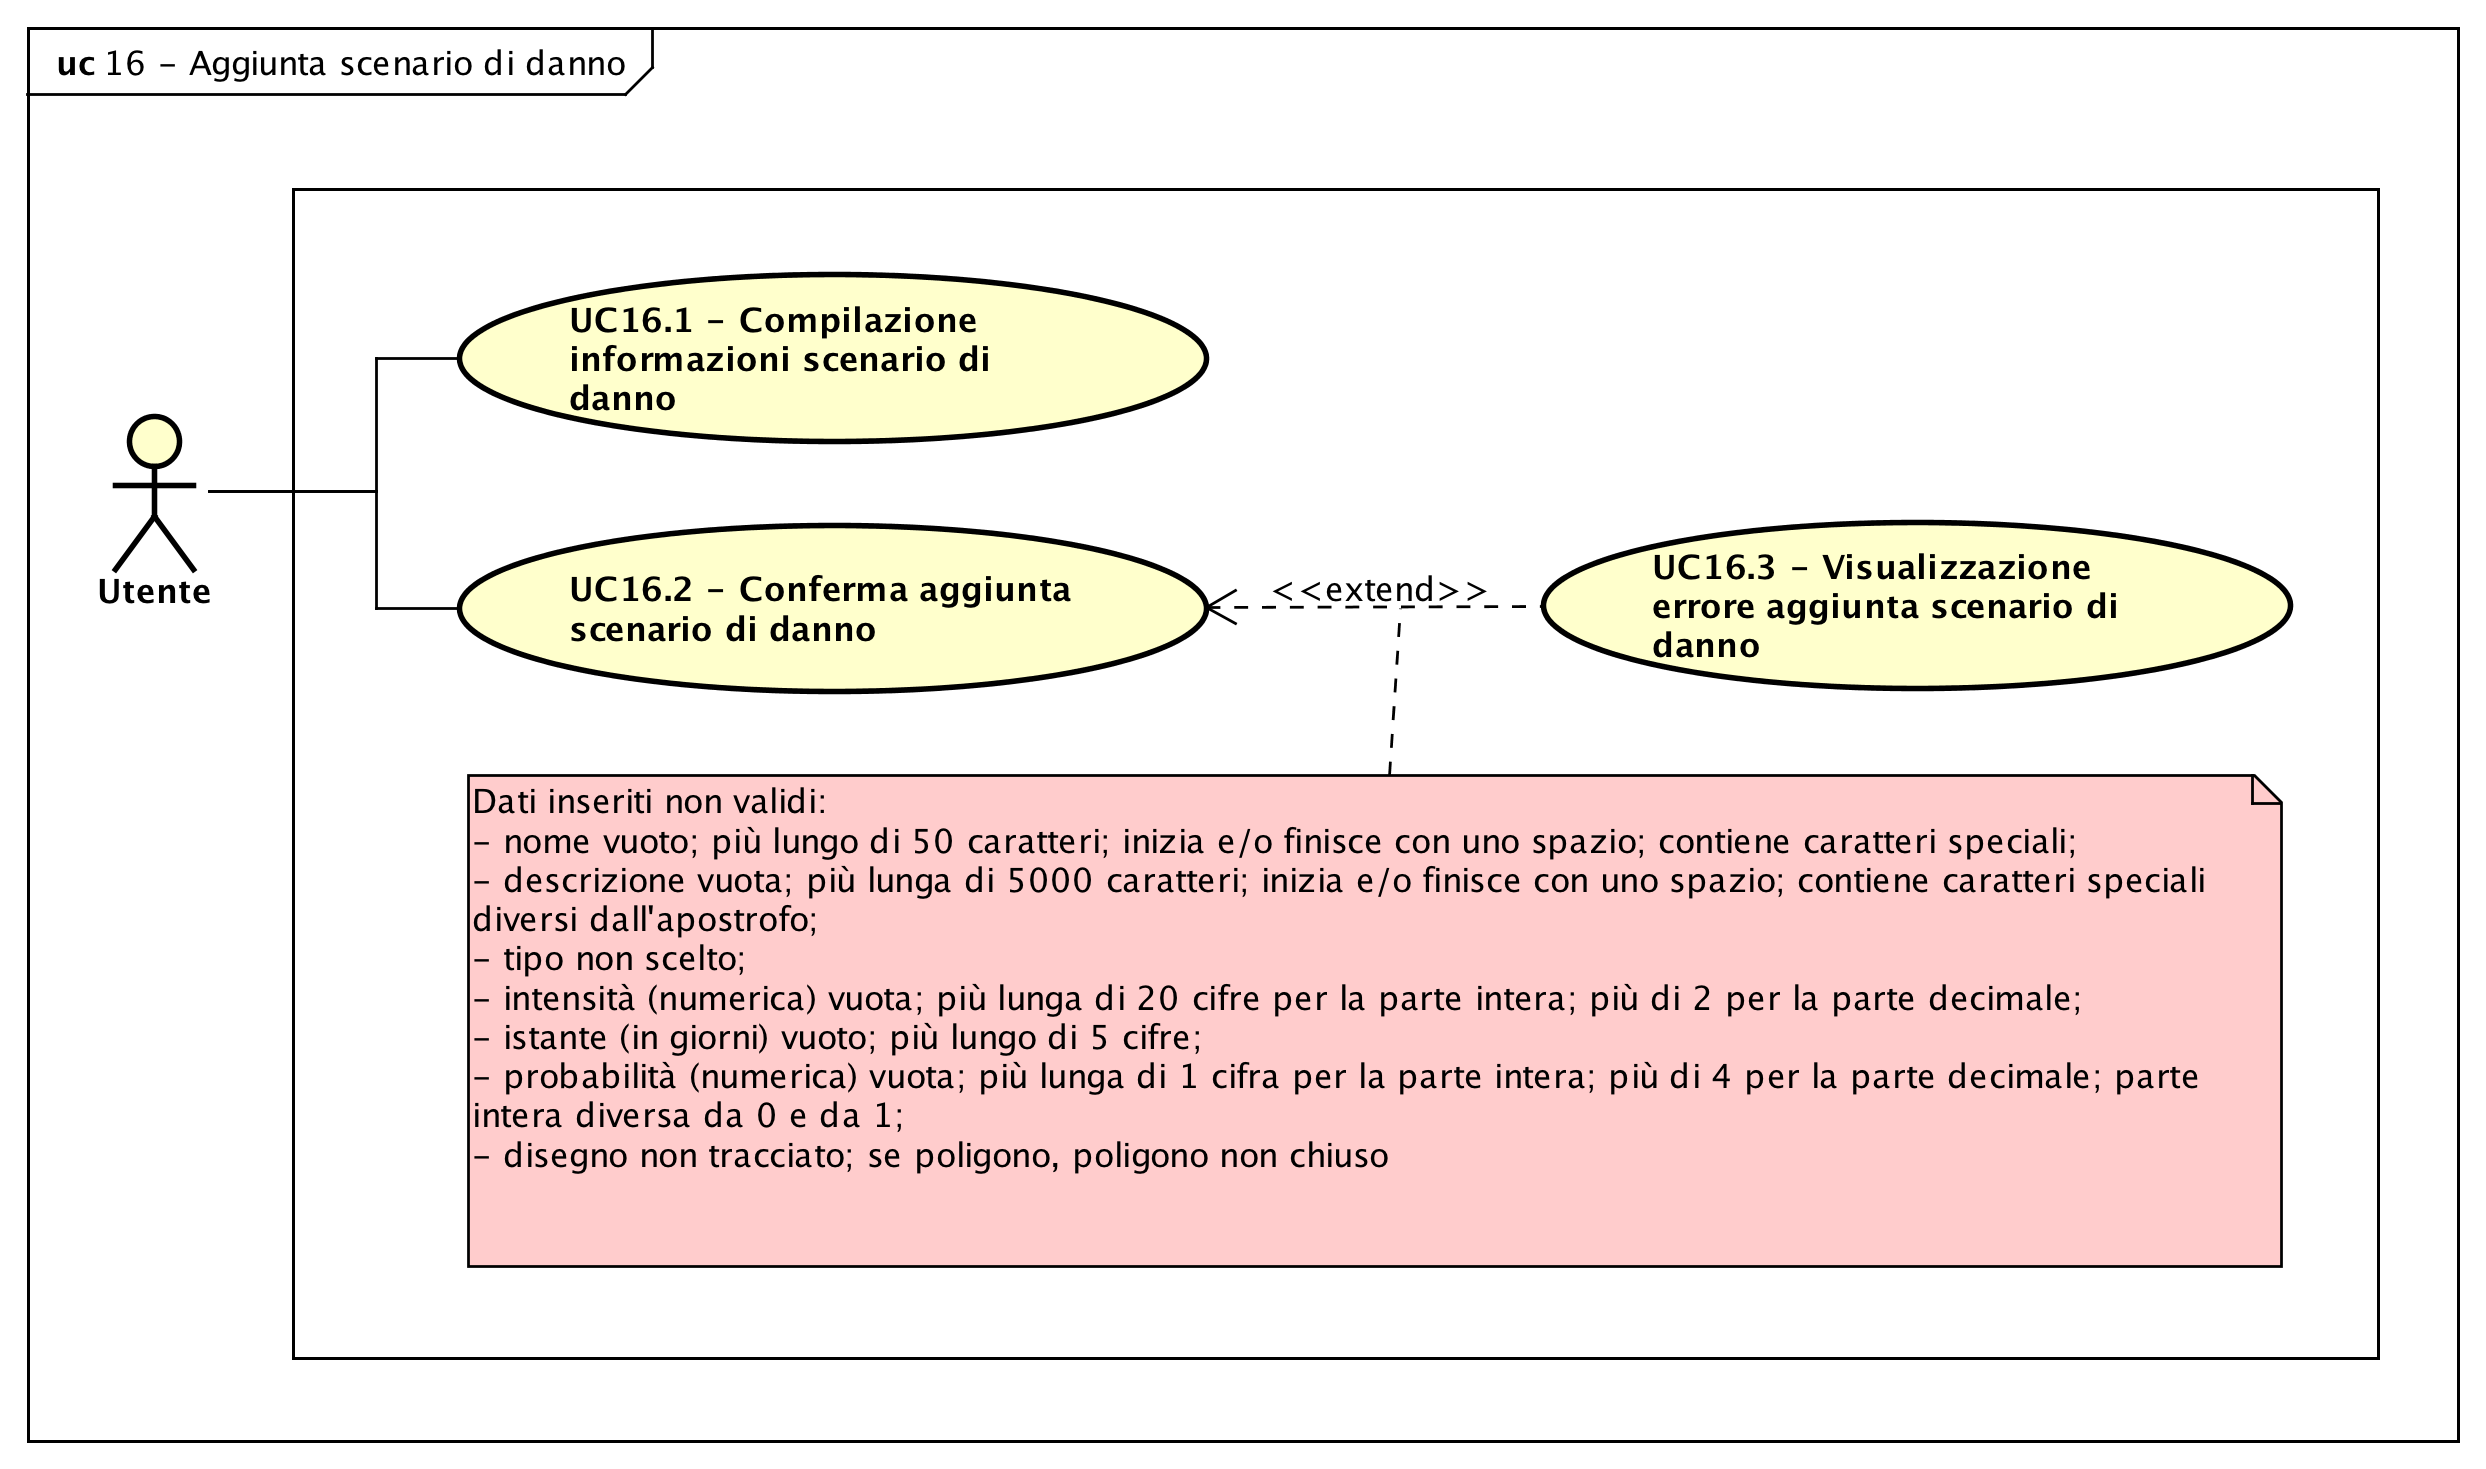
\includegraphics[width=\textwidth]{{img/uc16}.png} 
	\caption{UC16 - Aggiunta scenario di danno}
\end{figure}
\def\arraystretch{1.5}
\rowcolors{2}{D}{P}
\begin{tabularx}{\textwidth}{l|p{0.7\textwidth}}
	\rowcolor{I} \multicolumn{2}{c}{\color{white}\textbf{UC16 - Aggiunta scenario di danno}} \\
	\toprule
	\endhead
	\textbf{Attori} & Utente\\
	\textbf{Descrizione} & l'utente aggiunge uno scenario di danno\\
	\textbf{Pre-condizione} & l'utente ha aperto l'applicazione\\
	\textbf{Post-condizione} & un nuovo scenario di danno è stato aggiunto ed è visualizzabile sulla mappa; l'utente visualizza un messaggio che comunica la corretta esecuzione dell'operazione; l'area informativa rimane impostata sullo scenario appena inserito; la posizione e il livello di ingrandimento della mappa rimangono invariati\\
	\textbf{Scenario principale} & \vspace{-1.2em}\begin{enumerate}[leftmargin=*,noitemsep,nosep]
		\item \nameref{sssec:UC16.1};
		\item \nameref{sssec:UC16.2}.
	\end{enumerate}\\
	\textbf{Estensioni} & \vspace{-1.2em}\begin{itemize}[leftmargin=*,noitemsep,nosep]
		\item \nameref{sssec:UC39}: l’utente interrompe volontariamente l’aggiunta dello
		scenario di danno;
	\end{itemize}\\
	\textbf{Scenari alternativi} & \vspace{-1.2em}\begin{itemize}[leftmargin=*,noitemsep,nosep]
		\item \nameref{sssec:UC16.3}.
	\end{itemize}\\
	%\textbf{Generalizzazioni} &  \\
	\bottomrule
\end{tabularx}
\subsection{UC16.1 - Compilazione informazioni scenario di danno} 
\label{sssec:UC16.1} 
\begin{figure}[H] 
	\centering 
	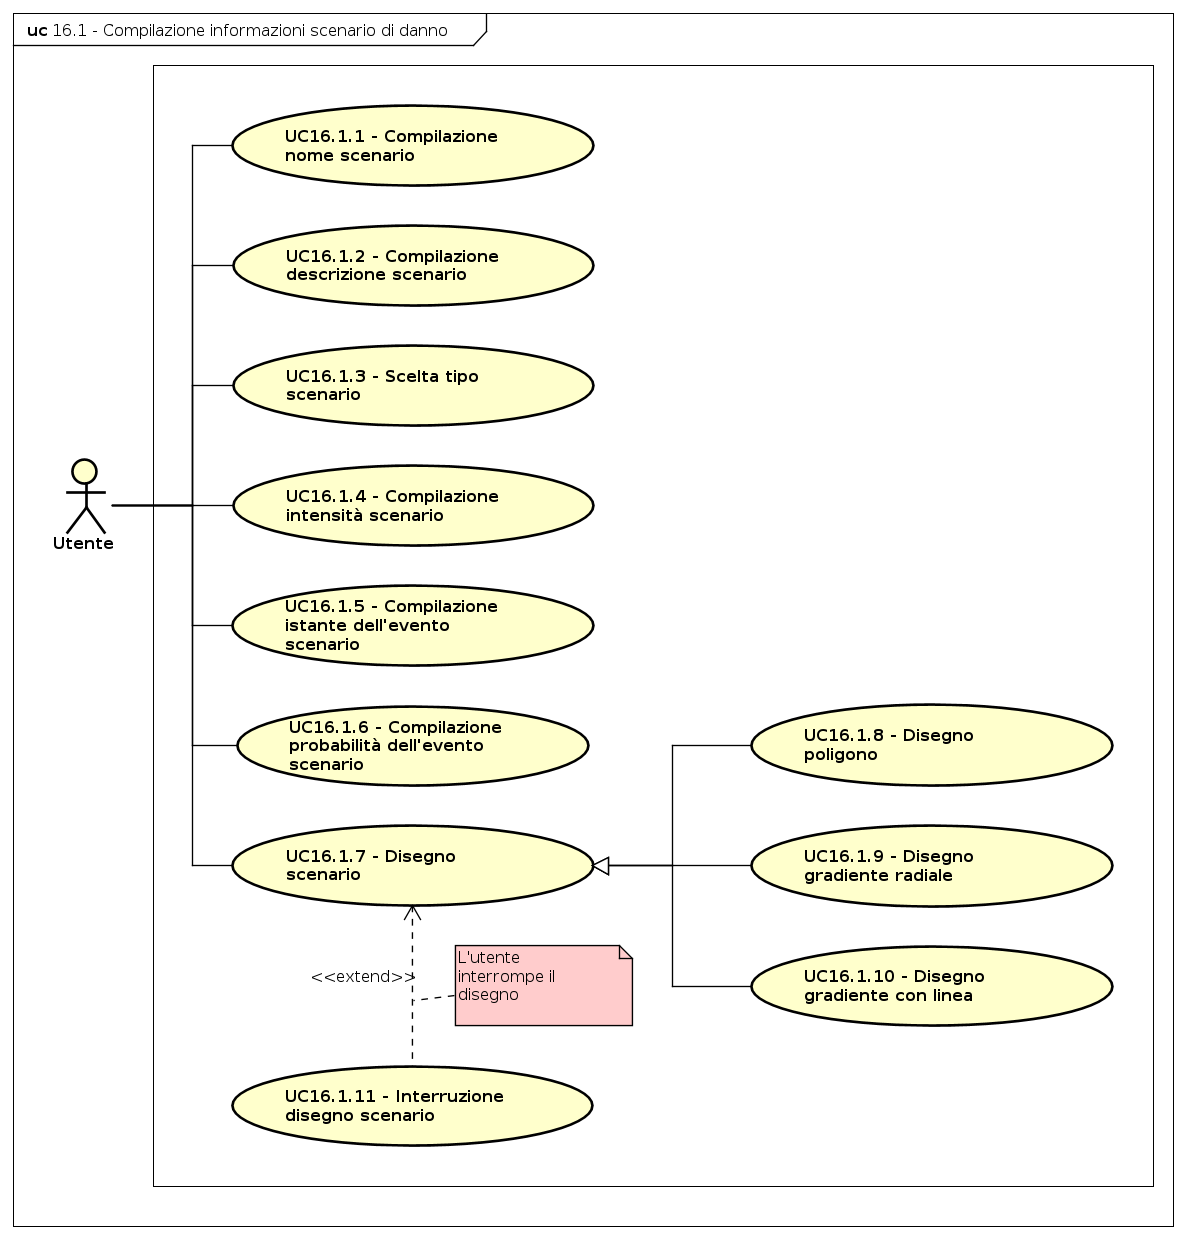
\includegraphics[width=\textwidth]{{img/uc16.1}.png} 
	\caption{UC16.1 - Compilazione informazioni scenario di danno}
\end{figure}
\def\arraystretch{1.5}
\rowcolors{2}{D}{P}
\begin{tabularx}{\textwidth}{l|p{0.7\textwidth}}
	\rowcolor{I} \multicolumn{2}{c}{\color{white}\textbf{UC16.1 - Compilazione informazioni scenario di danno}} \\
	\toprule
	\endhead
	\textbf{Attori} & Utente\\
	\textbf{Descrizione} & l'utente compila le informazioni dello scenario di danno\\
	\textbf{Pre-condizione} & il sistema offre la possbilità di compilare le informazioni dello scenario di danno\\
	\textbf{Post-condizione} & le informazioni dello scenario di danno sono state compilate e sono visualizzabili nell'area informativa; l'utente viene riportato alla schermata di aggiunta scenario, dove può confermarne l'aggiunta\\
	\textbf{Scenario principale} & \vspace{-1.2em}\begin{enumerate}[leftmargin=*,noitemsep,nosep]
		\item \nameref{sssec:UC16.1.1};
		\item \nameref{sssec:UC16.1.2};
		\item \nameref{sssec:UC16.1.3};
		\item \nameref{sssec:UC16.1.4};
		\item \nameref{sssec:UC16.1.5};
		\item \nameref{sssec:UC16.1.6};
		\item \nameref{sssec:UC16.1.8} oppure
		\item \nameref{sssec:UC16.1.9} oppure
		\item \nameref{sssec:UC16.1.10}.
	\end{enumerate}\\
	\textbf{Scenari alternativi} & \vspace{-1.2em}\begin{itemize}[leftmargin=*,noitemsep,nosep]
	\item \nameref{sssec:UC16.1.11}: : l’utente interrompe volontariamente il disegno dello
	scenario di danno
\end{itemize}\\
	%\textbf{Generalizzazioni} &  \\
	\bottomrule
\end{tabularx}
\subsection{UC16.1.1 - Compilazione nome scenario} 
\label{sssec:UC16.1.1} 
\def\arraystretch{1.5}
\rowcolors{2}{D}{P}
\begin{tabularx}{\textwidth}{l|p{0.7\textwidth}}
	\rowcolor{I} \multicolumn{2}{c}{\color{white}\textbf{UC16.1.1 - Compilazione nome scenario}} \\
	\toprule
	\endhead
	\textbf{Attori} & Utente\\
	\textbf{Descrizione} & l'utente compila il nome dello scenario\\
	\textbf{Pre-condizione} & il sistema offre la possibilità di compilare il nome dello scenario\\
	\textbf{Post-condizione} & l'utente ha compilato il nome dello scenario e può visualizzare il nome appena inserito nell'area informativa\\
	\textbf{Scenario principale} & \vspace{-1.2em}\begin{enumerate}[leftmargin=*,noitemsep,nosep]
		\item \nameref{sssec:UC16.1.1}.
	\end{enumerate}\\
	%\textbf{Generalizzazioni} &  \\
	\bottomrule
\end{tabularx}

\subsection{UC16.1.2 - Compilazione descrizione scenario} 
\label{sssec:UC16.1.2} 
\def\arraystretch{1.5}
\rowcolors{2}{D}{P}
\begin{tabularx}{\textwidth}{l|p{0.7\textwidth}}
	\rowcolor{I} \multicolumn{2}{c}{\color{white}\textbf{UC16.1.2 - Compilazione descrizione scenario}} \\
	\toprule
	\endhead
	\textbf{Attori} & Utente\\
	\textbf{Descrizione} & l'utente compila la descrizione dello scenario\\
	\textbf{Pre-condizione} & il sistema offre la possibilità di compilare la descrizione dello scenario\\
	\textbf{Post-condizione} & l'utente ha compilato la descrizione dello scenario e visualizza la descrizione appena compilata nell'area informativa\\
	\textbf{Scenario principale} & \vspace{-1.2em}\begin{enumerate}[leftmargin=*,noitemsep,nosep]
		\item \nameref{sssec:UC16.1.2}.
	\end{enumerate}\\
	%\textbf{Generalizzazioni} &  \\
	\bottomrule
\end{tabularx}
\subsection{UC16.1.3 - Scelta tipo scenario} 
\label{sssec:UC16.1.3} 
\def\arraystretch{1.5}
\rowcolors{2}{D}{P}
\begin{tabularx}{\textwidth}{l|p{0.7\textwidth}}
	\rowcolor{I} \multicolumn{2}{c}{\color{white}\textbf{UC16.1.3 - Scelta tipo scenario}} \\
	\toprule
	\endhead
	\textbf{Attori} & Utente\\
	\textbf{Descrizione} & l'utente sceglie il tipo di scenario\\
	\textbf{Pre-condizione} & il sistema offre la possibilità di scegliere il tipo di scenario\\
	\textbf{Post-condizione} & il tipo di scenario è stato scelto e l'utente visualizza il tipo appena scelto nell'area informativa\\
	\textbf{Scenario principale} & \vspace{-1.2em}\begin{enumerate}[leftmargin=*,noitemsep,nosep]
		\item \nameref{sssec:UC16.1.3}.
	\end{enumerate}\\
	%\textbf{Generalizzazioni} &  \\
	\bottomrule
\end{tabularx}
\subsection{UC16.1.4 - Compilazione intensità scenario} 
\label{sssec:UC16.1.4} 
\def\arraystretch{1.5}
\rowcolors{2}{D}{P}
\begin{tabularx}{\textwidth}{l|p{0.7\textwidth}}
	\rowcolor{I} \multicolumn{2}{c}{\color{white}\textbf{UC16.1.4 - Compilazione intensità scenario}} \\
	\toprule
	\endhead
	\textbf{Attori} & Utente\\
	\textbf{Descrizione} & l'utente compila l'intensità dello scenario\\
	\textbf{Pre-condizione} & il sistema offre la possibilità di compilare l'intensità dello scenario\\
	\textbf{Post-condizione} & l'utente ha compilato l'intensità dello scenario e visualizza l'intensità appena compilata nell'area informativa\\
	\textbf{Scenario principale} & \vspace{-1.2em}\begin{enumerate}[leftmargin=*,noitemsep,nosep]
		\item \nameref{sssec:UC16.1.4}.
	\end{enumerate}\\
	%\textbf{Generalizzazioni} &  \\
	\bottomrule
\end{tabularx}
\subsection{UC16.1.5 - Compilazione istante dell'evento scenario} 
\label{sssec:UC16.1.5} 
\def\arraystretch{1.5}
\rowcolors{2}{D}{P}
\begin{tabularx}{\textwidth}{l|p{0.7\textwidth}}
	\rowcolor{I} \multicolumn{2}{c}{\color{white}\textbf{UC16.1.5 - Compilazione istante dell'evento scenario}} \\
	\toprule
	\endhead
	\textbf{Attori} & Utente\\
	\textbf{Descrizione} & l'utente compila l'istante dell'evento dello scenario\\
	\textbf{Pre-condizione} & il sistema offre la possibilità di compilare l'istante dell'evento dello scenario\\
	\textbf{Post-condizione} & l'istante dell'evento dello scenario è stato compilato e l'utente visualizza l'istante appena compilato nell'area informativa\\
	\textbf{Scenario principale} & \vspace{-1.2em}\begin{enumerate}[leftmargin=*,noitemsep,nosep]
		\item \nameref{sssec:UC16.1.5}.
	\end{enumerate}\\
	%\textbf{Generalizzazioni} &  \\
	\bottomrule
\end{tabularx}
\subsection{UC16.1.6 - Compilazione probabilità dell'evento scenario} 
\label{sssec:UC16.1.6} 
\def\arraystretch{1.5}
\rowcolors{2}{D}{P}
\begin{tabularx}{\textwidth}{l|p{0.7\textwidth}}
	\rowcolor{I} \multicolumn{2}{c}{\color{white}\textbf{UC16.1.6 - Compilazione probabilità dell'evento scenario}} \\
	\toprule
	\endhead
	\textbf{Attori} & Utente\\
	\textbf{Descrizione} & l'utente compila la probabilità dell'evento dello scenario\\
	\textbf{Pre-condizione} & il sistema offre la possibilità di compilare la probabilità dell'evento dello scenario\\
	\textbf{Post-condizione} & la probabilità dell'evento dello scenario è stata compilata e l'utente visualizza la probabilità appena compilata nell'area informativa\\
	\textbf{Scenario principale} & \vspace{-1.2em}\begin{enumerate}[leftmargin=*,noitemsep,nosep]
		\item \nameref{sssec:UC16.1.6}.
	\end{enumerate}\\
	%\textbf{Generalizzazioni} &  \\
	\bottomrule
\end{tabularx}
	\subsection{UC16.1.7 - Disegno scenario} 
\label{sssec:UC16.1.7} 
\def\arraystretch{1.5}
\rowcolors{2}{D}{P}
\begin{tabularx}{\textwidth}{l|p{0.7\textwidth}}
	\rowcolor{I} \multicolumn{2}{c}{\color{white}\textbf{UC16.1.7 - Disegno scenario}} \\
	\toprule
	\endhead
	\textbf{Attori} & Utente\\
	\textbf{Descrizione} & l'utente disegna lo scenario di danno\\
	\textbf{Pre-condizione} & il sistema offre la possibilità di disegnare lo scenario di danno\\
	\textbf{Post-condizione} & lo scenario di danno è stato disegnato e viene visualizzato sulla mappa\\
	\textbf{Scenario principale} & \vspace{-1.2em}\begin{enumerate}[leftmargin=*,noitemsep,nosep]
		\item \nameref{sssec:UC16.1.7}.
	\end{enumerate}\\
	\textbf{Estensioni} & \vspace{-1.2em}\begin{itemize}[leftmargin=*,noitemsep,nosep]
		\item \nameref{sssec:UC16.1.11}: l’utente interrompe volontariamente il disegno dello
		scenario di danno
	\end{itemize}\\
	\textbf{Generalizzazioni} &
	\vspace{-1.2em}\begin{itemize}
		[leftmargin=*,noitemsep,nosep]
		\item \nameref{sssec:UC16.1.8};
		\item \nameref{sssec:UC16.1.9};
		\item \nameref{sssec:UC16.1.10};
	\end{itemize} \\
	
	\bottomrule
\end{tabularx}
\subsection{UC16.1.8 - Disegno poligono} 
\label{sssec:UC16.1.8} 
\def\arraystretch{1.5}
\rowcolors{2}{D}{P}
\begin{tabularx}{\textwidth}{l|p{0.7\textwidth}}
	\rowcolor{I} \multicolumn{2}{c}{\color{white}\textbf{UC16.1.8 - Disegno poligono}} \\
	\toprule
	\endhead
	\textbf{Attori} & Utente\\
	\textbf{Descrizione} & l'utente disegna lo scenario mediante poligono\\
	\textbf{Pre-condizione} & il sistema offre la possibilità di disegnare lo scenario\\
	\textbf{Post-condizione} & lo scenario è stato disegnato mediante poligono e viene visualizzato sulla mappa\\
	\textbf{Scenario principale} & \vspace{-1.2em}\begin{enumerate}[leftmargin=*,noitemsep,nosep]
		\item \nameref{sssec:UC16.1.8}.
	\end{enumerate}\\
	%\textbf{Generalizzazioni} &  \\
	\bottomrule
\end{tabularx}
\subsection{UC16.1.9 - Disegno gradiente radiale} 
\label{sssec:UC16.1.9} 
\def\arraystretch{1.5}
\rowcolors{2}{D}{P}
\begin{tabularx}{\textwidth}{l|p{0.7\textwidth}}
	\rowcolor{I} \multicolumn{2}{c}{\color{white}\textbf{UC16.1.9 - Disegno gradiente radiale}} \\
	\toprule
	\endhead
	\textbf{Attori} & Utente\\
	\textbf{Descrizione} & l'utente disegna lo scenario di danno mediante gradiente radiale\\
	\textbf{Pre-condizione} & il sistema offre la possibilità di disegnare lo scenario\\
	\textbf{Post-condizione} & lo scenario è stato disegnato mediante gradiente radiale e viene visualizzato sulla mappa\\
	\textbf{Scenario principale} & \vspace{-1.2em}\begin{enumerate}[leftmargin=*,noitemsep,nosep]
		\item \nameref{sssec:UC16.1.9}.
	\end{enumerate}\\
	%\textbf{Generalizzazioni} &  \\
	\bottomrule
\end{tabularx}
\subsection{UC16.1.10 - Disegno gradiente con linea} 
\label{sssec:UC16.1.10} 
\def\arraystretch{1.5}
\rowcolors{2}{D}{P}
\begin{tabularx}{\textwidth}{l|p{0.7\textwidth}}
	\rowcolor{I} \multicolumn{2}{c}{\color{white}\textbf{UC16.1.10 - Disegno gradiente con linea}} \\
	\toprule
	\endhead
	\textbf{Attori} & Utente\\
	\textbf{Descrizione} & l'utente disegna lo scenario di danno mediante gradiente con linea\\
	\textbf{Pre-condizione} & il sistema offre la possibilità di disegnare lo scenario\\
	\textbf{Post-condizione} & lo scenario è stato disegnato mediante gradiente con linea; l'utente può visualizzare il gradiente sulla mappa\\
	\textbf{Scenario principale} & \vspace{-1.2em}\begin{enumerate}[leftmargin=*,noitemsep,nosep]
		\item \nameref{sssec:UC16.1.10}.
	\end{enumerate}\\
	%\textbf{Generalizzazioni} &  \\
	\bottomrule
\end{tabularx}
\subsection{UC16.1.11 - Interruzione disegno scenario} 
\label{sssec:UC16.1.11} 
\def\arraystretch{1.5}
\rowcolors{2}{D}{P}
\begin{tabularx}{\textwidth}{l|p{0.7\textwidth}}
	\rowcolor{I} \multicolumn{2}{c}{\color{white}\textbf{UC16.1.11 - Interruzione disegno scenario}} \\
	\toprule
	\endhead
	\textbf{Attori} & Utente\\
	\textbf{Descrizione} & l'utente interrompe il disegno dello scenario\\
	\textbf{Pre-condizione} & il sistema offre la possibilità di disegnare lo scenario\\
	\textbf{Post-condizione} & lo scenario non è stato disegnato; l'utente viene riportato alla schermata di inserimento scenario\\
	\textbf{Scenario principale} & \vspace{-1.2em}\begin{enumerate}[leftmargin=*,noitemsep,nosep]
		\item \nameref{sssec:UC16.1.11}.
	\end{enumerate}\\
	%\textbf{Generalizzazioni} &  \\
	\bottomrule
\end{tabularx}
\subsection{UC16.2 - Conferma aggiunta scenario di danno} 
\label{sssec:UC16.2} 
\def\arraystretch{1.5}
\rowcolors{2}{D}{P}
\begin{tabularx}{\textwidth}{l|p{0.7\textwidth}}
	\rowcolor{I} \multicolumn{2}{c}{\color{white}\textbf{UC16.2 - Conferma aggiunta scenario di danno}} \\
	\toprule
	\endhead
	\textbf{Attori} & Utente\\
	\textbf{Descrizione} & l'utente conferma l'aggiunta dello scenario di danno\\
	\textbf{Pre-condizione} & il sistema offre la possibilità di confermare l'aggiunta dello scenario di danno\\
	\textbf{Post-condizione} & un nuovo scenario di danno è stato aggiunto ma non viene visualizzato sulla mappa; l'utente visualizza un messaggio che comunica la corretta esecuzione dell'operazione; l'area informativa viene impostata alla visualizzazione di default; la posizione e il livello di ingrandimento della mappa rimangono invariati\\
	\textbf{Scenario principale} & \vspace{-1.2em}\begin{enumerate}[leftmargin=*,noitemsep,nosep]
		\item \nameref{sssec:UC16.2}.
	\end{enumerate}\\
	\textbf{Estensioni} & \vspace{-1.2em}\begin{itemize}[leftmargin=*,noitemsep,nosep]
		\item \nameref{sssec:UC16.3}: dati inseriti non validi:
		\begin{itemize}
			\item nome vuoto; più lungo di 50 caratteri; inizia e/o
			finisce con uno spazio; contiene caratteri speciali;
			\item descrizione vuota; più lunga di 5000 caratteri;
			inizia e/o finisce con uno spazio; contiene
			caratteri speciali diversi dall'apostrofo;
			\item tipo non scelto;
			\item intensità (numerica) vuota; più lunga di 20 cifre per la
			parte intera; più di 2 per la parte decimale;
			\item istante (in giorni) vuoto; più lungo di 5 cifre;
			\item probabilità (numerica) vuota; più lunga di 1 cifra per la
			parte intera; più di 4 per la parte decimale; parte
			intera diversa da 0 e da 1;
			\item disegno non tracciato; se poligono, poligono non
			chiuso
		\end{itemize}
	\end{itemize}\\
	%\textbf{Generalizzazioni} &  \\
	\bottomrule
\end{tabularx}
\subsection{UC16.3 - Visualizzazione errore aggiunta scenario di danno} 
\label{sssec:UC16.3} 
\def\arraystretch{1.5}
\rowcolors{2}{D}{P}
\begin{tabularx}{\textwidth}{l|p{0.7\textwidth}}
	\rowcolor{I} \multicolumn{2}{c}{\color{white}\textbf{UC16.3 - Visualizzazione errore aggiunta scenario di danno}} \\
	\toprule
	\endhead
	\textbf{Attori} & Utente\\
	\textbf{Descrizione} & l'utente visualizza un errore relativo ai dati dello scenario di danno compilati in modo errato\\
	\textbf{Pre-condizione} & l'utente sta tentando di inserire un nuovo scenario di danno\\
	\textbf{Post-condizione} & nessun nuovo scenario di danno inserito;  l'utente visualizza un errore relativo ai dati dello scenario di danno compilati in modo errato; l'utente viene riportato alla schermata di aggiunta scenario\\
	\textbf{Scenario principale} & \vspace{-1.2em}\begin{enumerate}[leftmargin=*,noitemsep,nosep]
		\item \nameref{sssec:UC16.3}.
	\end{enumerate}\\
	%\textbf{Generalizzazioni} &  \\
	\bottomrule
\end{tabularx}
\subsection{UC17 - Scelta visualizzazione scenario di danno} 
\label{sssec:UC17} 
\def\arraystretch{1.5}
\rowcolors{2}{D}{P}
\begin{tabularx}{\textwidth}{l|p{0.7\textwidth}}
	\rowcolor{I} \multicolumn{2}{c}{\color{white}\textbf{UC17 - Scelta visualizzazione scenario di danno}} \\
	\toprule
	\endhead
	\textbf{Attori} & Utente\\
	\textbf{Descrizione} & l'utente sceglie quale scenario di danno visualizzare\\
	\textbf{Pre-condizione} & l'utente ha aperto l'applicazione; almeno uno scenario di danno è stato inserito\\
	\textbf{Post-condizione} & il sistema mostra nell'area informativa le informazioni dello scenario di danno selezionato; la posizione e il livello di ingrandimento della mappa rimangono invariati\\
	\textbf{Scenario principale} & \vspace{-1.2em}\begin{enumerate}[leftmargin=*,noitemsep,nosep]
		\item \nameref{sssec:UC17}.
	\end{enumerate}\\
	%\textbf{Generalizzazioni} &  \\
	\bottomrule
\end{tabularx}
\subsection{UC18 - Chiusura visualizzazione scenario di danno} 
\label{sssec:UC18} 
\def\arraystretch{1.5}
\rowcolors{2}{D}{P}
\begin{tabularx}{\textwidth}{l|p{0.7\textwidth}}
	\rowcolor{I} \multicolumn{2}{c}{\color{white}\textbf{UC18 - Chiusura visualizzazione scenario di danno}} \\
	\toprule
	\endhead
	\textbf{Attori} & Utente\\
	\textbf{Descrizione} & l'utente chiude la visualizzazione dello scenario di danno\\
	\textbf{Pre-condizione} & l'utente ha aperto l'applicazione; uno scenario di danno è visualizzato sulla mappa\\
	\textbf{Post-condizione} & è stata chiusa la visualizzazione delle informazioni dello scenario di danno selezionato nell'area informativa; l'area informativa viene impostata sulla visualizzazione di default; la posizione e il livello di ingrandimento della mappa rimangono invariati\\
	\textbf{Scenario principale} & \vspace{-1.2em}\begin{enumerate}[leftmargin=*,noitemsep,nosep]
		\item \nameref{sssec:UC18}.
	\end{enumerate}\\
	%\textbf{Generalizzazioni} &  \\
	\bottomrule
\end{tabularx}
\subsection{UC19 - Modifica scenario di danno} 
\label{sssec:UC19} 
\begin{figure}[H] 
	\centering 
	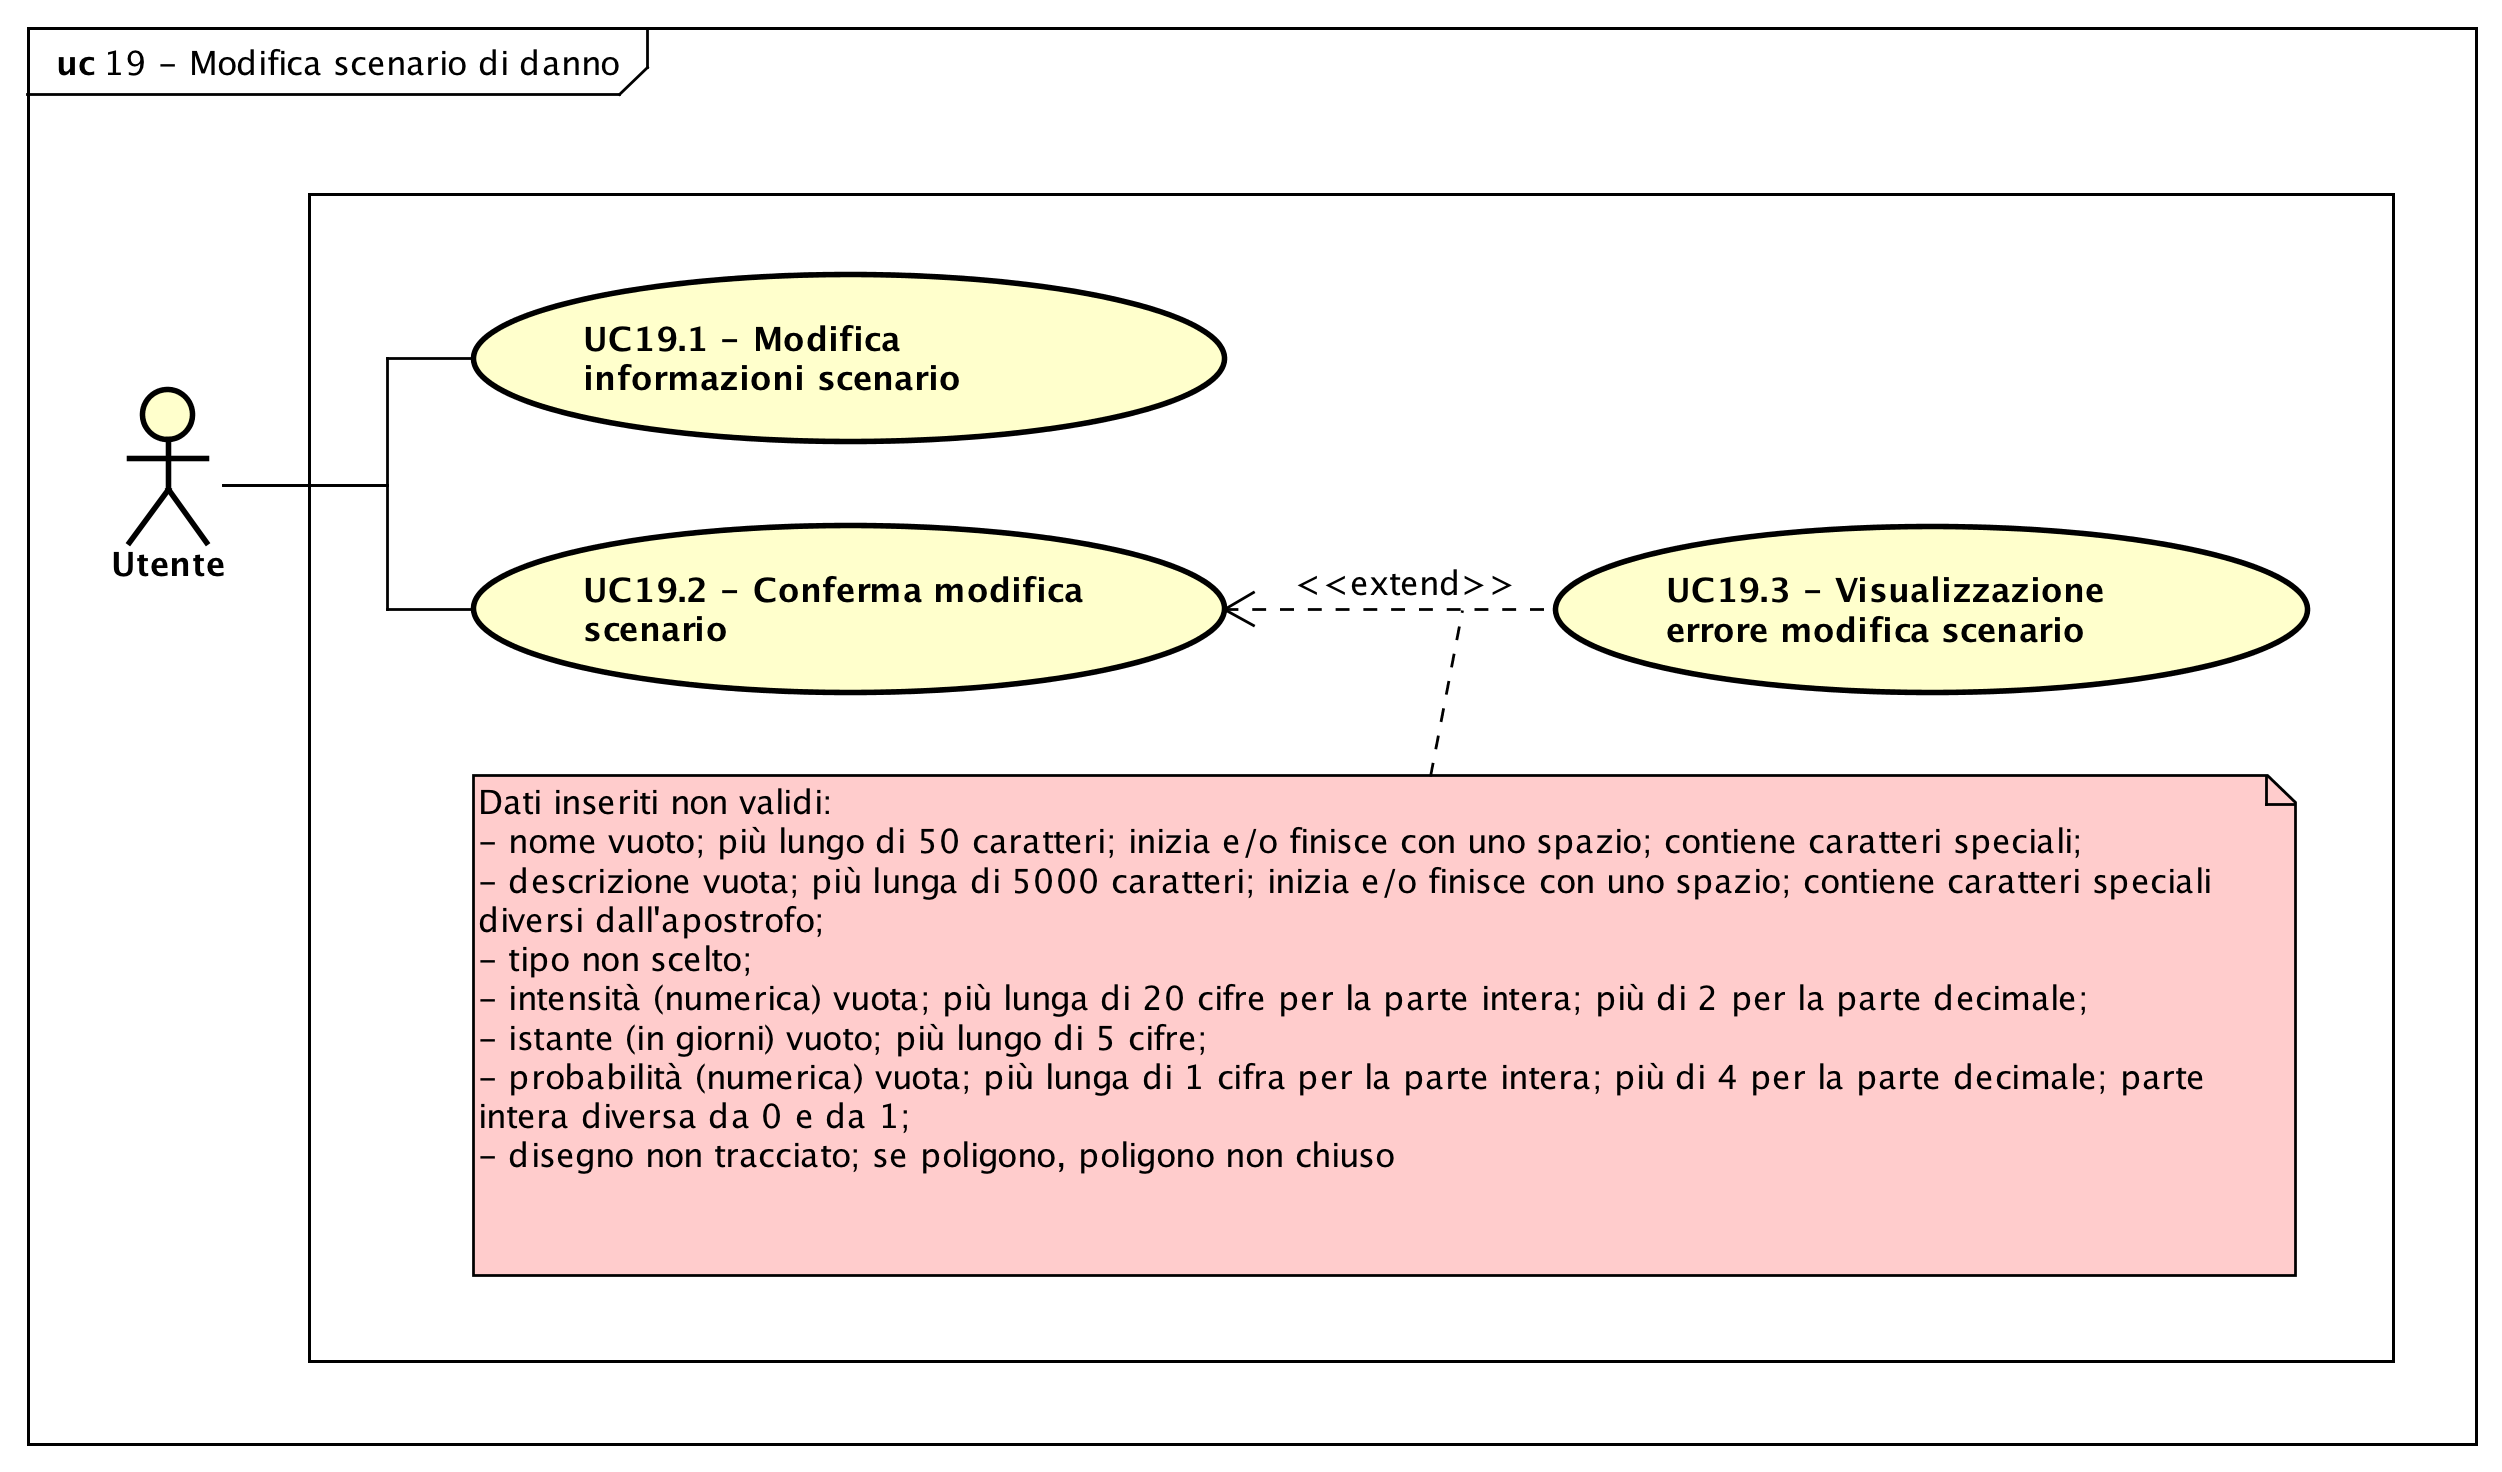
\includegraphics[width=\textwidth]{{img/uc19}.png} 
	\caption{UC19 - Modifica scenario di danno}
\end{figure}
\def\arraystretch{1.5}
\rowcolors{2}{D}{P}
\begin{tabularx}{\textwidth}{l|p{0.7\textwidth}}
	\rowcolor{I} \multicolumn{2}{c}{\color{white}\textbf{UC19 - Modifica scenario di danno}} \\
	\toprule
	\endhead
	\textbf{Attori} & Utente\\
	\textbf{Descrizione} & l'utente modifica lo scenario di danno\\
	\textbf{Pre-condizione} & l'utente ha aperto l'applicazione; almeno uno scenario di danno è stato aggiunto; l'utente ha selezionato uno scenario di danno\\
	\textbf{Post-condizione} & lo scenario di danno è stato modificato; l'utente viisualizza un messaggio che comunica la corretta esecuzione dell'operazione; l'area informativa rimane impostata sullo scenario appena modificato; la posizione e il livello di ingrandimento della mappa rimangono invariati\\
	\textbf{Scenario principale} & \vspace{-1.2em}\begin{enumerate}[leftmargin=*,noitemsep,nosep]
		\item \nameref{sssec:UC19.1};
		\item \nameref{sssec:UC19.2}.
	\end{enumerate}\\
	\textbf{Estensioni} & \vspace{-1.2em}\begin{itemize}[leftmargin=*,noitemsep,nosep]
		\item \nameref{sssec:UC40}: l’utente interrompe volontariamente la modifica dello
		scenario di danno
	\end{itemize}\\
	\textbf{Scenari alternativi} & \vspace{-1.2em}\begin{itemize}[leftmargin=*,noitemsep,nosep]
		\item \nameref{sssec:UC19.3}.
	\end{itemize}\\
	%\textbf{Generalizzazioni} &  \\
	\bottomrule
\end{tabularx}
\subsection{UC19.1 - Modifica informazioni scenario} 
\label{sssec:UC19.1} 
\begin{figure}[H] 
	\centering 
	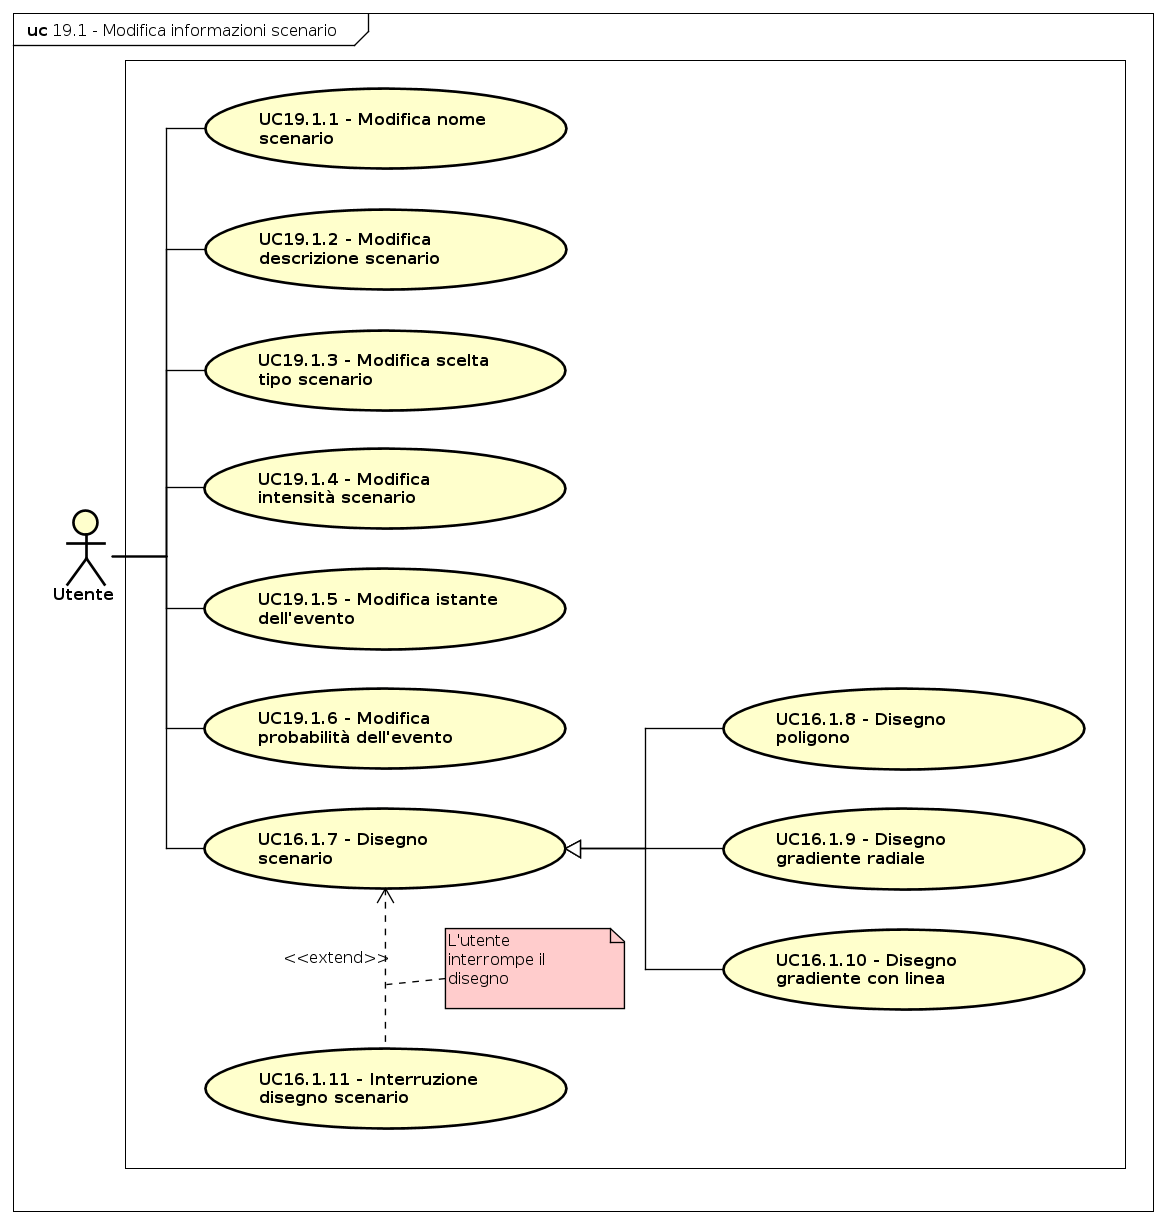
\includegraphics[width=\textwidth]{{img/uc19.1}.png} 
	\caption{UC4 - Modifica informazioni scenario}
\end{figure}
\def\arraystretch{1.5}
\rowcolors{2}{D}{P}
\begin{tabularx}{\textwidth}{l|p{0.7\textwidth}}
	\rowcolor{I} \multicolumn{2}{c}{\color{white}\textbf{UC19.1 - Modifica informazioni scenario}} \\
	\toprule
	\endhead
	\textbf{Attori} & Utente\\
	\textbf{Descrizione} & l'utente modifica le informazioni dello scenario\\
	\textbf{Pre-condizione} & il sistema offre la possibilità di modificare le informazioni dello scenario\\
	\textbf{Post-condizione} & le informazioni dello scenario sono state modificate; l'utente viene riportato alla schermata di modifica scenario, dove può confermare la modifica\\
	\textbf{Scenario principale} & \vspace{-1.2em}\begin{enumerate}[leftmargin=*,noitemsep,nosep]
		\item \nameref{sssec:UC19.1.1};
		\item \nameref{sssec:UC19.1.2};
		\item \nameref{sssec:UC19.1.3};
		\item \nameref{sssec:UC19.1.4};
		\item \nameref{sssec:UC19.1.5};
		\item \nameref{sssec:UC19.1.6};
		\item \nameref{sssec:UC16.1.8} oppure
		\item \nameref{sssec:UC16.1.9} oppure
		\item \nameref{sssec:UC16.1.10}.
	\end{enumerate}\\
\textbf{Scenari alternativi} & \vspace{-1.2em}\begin{itemize}[leftmargin=*,noitemsep,nosep]
	\item \nameref{sssec:UC16.1.11}: : l’utente interrompe volontariamente il disegno dello
	scenario di danno
\end{itemize}\\
	%\textbf{Generalizzazioni} &  \\
	\bottomrule
\end{tabularx}
\subsection{UC19.1.1 - Modifica nome scenario} 
\label{sssec:UC19.1.1} 
\def\arraystretch{1.5}
\rowcolors{2}{D}{P}
\begin{tabularx}{\textwidth}{l|p{0.7\textwidth}}
	\rowcolor{I} \multicolumn{2}{c}{\color{white}\textbf{UC19.1.1 - Modifica nome scenario}} \\
	\toprule
	\endhead
	\textbf{Attori} & Utente\\
	\textbf{Descrizione} & l'utente modifica il campo relativo al nome dello scenario\\
	\textbf{Pre-condizione} & il sistema offre la possibilità di modificare il nome dello scenario\\
	\textbf{Post-condizione} & il campo relativo al nome dello scenario è stato modificato; l'utente visualizza il nome appena inserito nell'area informativa\\
	\textbf{Scenario principale} & \vspace{-1.2em}\begin{enumerate}[leftmargin=*,noitemsep,nosep]
		\item \nameref{sssec:UC19.1.1}.
	\end{enumerate}\\
	%\textbf{Generalizzazioni} &  \\
	\bottomrule
\end{tabularx}
\subsection{UC19.1.2 - Modifica descrizione scenario} 
\label{sssec:UC19.1.2} 
\def\arraystretch{1.5}
\rowcolors{2}{D}{P}
\begin{tabularx}{\textwidth}{l|p{0.7\textwidth}}
	\rowcolor{I} \multicolumn{2}{c}{\color{white}\textbf{UC19.1.2 - Modifica descrizione scenario}} \\
	\toprule
	\endhead
	\textbf{Attori} & Utente\\
	\textbf{Descrizione} & l'utente modifica il campo relativo alla descrizione dello scenario\\
	\textbf{Pre-condizione} & il sistema offre la possibilità di modifica la descrizione dello scenario\\
	\textbf{Post-condizione} & il campo relativo alla descrizione dello scenario  è stato modificato; l'utente visualizza la descrizione appena inserita nell'area informativa\\
	\textbf{Scenario principale} & \vspace{-1.2em}\begin{enumerate}[leftmargin=*,noitemsep,nosep]
		\item \nameref{sssec:UC19.1.2}.
	\end{enumerate}\\
	%\textbf{Generalizzazioni} &  \\
	\bottomrule
\end{tabularx}
\subsection{UC19.1.3 - Modifica scelta tipo scenario} 
\label{sssec:UC19.1.3} 
\def\arraystretch{1.5}
\rowcolors{2}{D}{P}
\begin{tabularx}{\textwidth}{l|p{0.7\textwidth}}
	\rowcolor{I} \multicolumn{2}{c}{\color{white}\textbf{UC19.1.3 - Modifica scelta tipo scenario}} \\
	\toprule
	\endhead
	\textbf{Attori} & Utente\\
	\textbf{Descrizione} & l'utente modifica la scelta del tipo di scenario\\
	\textbf{Pre-condizione} & il sistema offre la possibilità di modificare la scelta del tipo di scenario\\
	\textbf{Post-condizione} & la scelta relativa al tipo dello scenario è stata modificata; l'utente visualizza il tipo di scenario appena scelto nell'area informativa\\
	\textbf{Scenario principale} & \vspace{-1.2em}\begin{enumerate}[leftmargin=*,noitemsep,nosep]
		\item \nameref{sssec:UC19.1.3}.
	\end{enumerate}\\
	%\textbf{Generalizzazioni} &  \\
	\bottomrule
\end{tabularx}
\subsection{UC19.1.4 - Modifica intensità scenario} 
\label{sssec:UC19.1.4} 
\def\arraystretch{1.5}
\rowcolors{2}{D}{P}
\begin{tabularx}{\textwidth}{l|p{0.7\textwidth}}
	\rowcolor{I} \multicolumn{2}{c}{\color{white}\textbf{UC19.1.4 - Modifica intensità scenario}} \\
	\toprule
	\endhead
	\textbf{Attori} & Utente\\
	\textbf{Descrizione} & l'utente modifica il campo relativo all'intensità dello scenario\\
	\textbf{Pre-condizione} & il sistema offre la possibilità di modificare l'intensità dello scenario\\
	\textbf{Post-condizione} & il campo relativo  all'intensità è stato modificato e l'utente visualizza l'intensità appena compilata nell'area informativa\\
	\textbf{Scenario principale} & \vspace{-1.2em}\begin{enumerate}[leftmargin=*,noitemsep,nosep]
		\item \nameref{sssec:UC19.1.4}.
	\end{enumerate}\\
	%\textbf{Generalizzazioni} &  \\
	\bottomrule
\end{tabularx}
\subsection{UC19.1.5 - Modifica istante dell'evento} 
\label{sssec:UC19.1.5} 
\def\arraystretch{1.5}
\rowcolors{2}{D}{P}
\begin{tabularx}{\textwidth}{l|p{0.7\textwidth}}
	\rowcolor{I} \multicolumn{2}{c}{\color{white}\textbf{UC19.1.5 - Modifica istante dell'evento}} \\
	\toprule
	\endhead
	\textbf{Attori} & Utente\\
	\textbf{Descrizione} & l'utente modifica il campo relativo all'istante dell'evento\\
	\textbf{Pre-condizione} & il sistema offre la possibilità di modificare l'istante dell'evento dello scenario\\
	\textbf{Post-condizione} & il campo relativo al nome all'istante dell'evento dello scenario è stato modificato; l'utente visualizza l'istante appena compilato nell'area informativa\\
	\textbf{Scenario principale} & \vspace{-1.2em}\begin{enumerate}[leftmargin=*,noitemsep,nosep]
		\item \nameref{sssec:UC19.1.5}.
	\end{enumerate}\\
	%\textbf{Generalizzazioni} &  \\
	\bottomrule
\end{tabularx}
\subsection{UC19.1.6 - Modifica probabilità dell'evento} 
\label{sssec:UC19.1.6} 
\def\arraystretch{1.5}
\rowcolors{2}{D}{P}
\begin{tabularx}{\textwidth}{l|p{0.7\textwidth}}
	\rowcolor{I} \multicolumn{2}{c}{\color{white}\textbf{UC19.1.6 - Modifica probabilità dell'evento}} \\
	\toprule
	\endhead
	\textbf{Attori} & Utente\\
	\textbf{Descrizione} & l'utente modifica la probabilità dell'evento dello scenario\\
	\textbf{Pre-condizione} & il sistema offre la possibilità di modificare la probabilità dell'evento dello scenario\\
	\textbf{Post-condizione} & la probabilità dell'evento dello scenario è stata modificata; l'utente visualizza la probabilità appena compilata nell'area informativa\\
	\textbf{Scenario principale} & \vspace{-1.2em}\begin{enumerate}[leftmargin=*,noitemsep,nosep]
		\item \nameref{sssec:UC19.1.6}.
	\end{enumerate}\\
	%\textbf{Generalizzazioni} &  \\
	\bottomrule
\end{tabularx}
\subsection{UC19.2 - Conferma modifica scenario} 
\label{sssec:UC19.2} 
\def\arraystretch{1.5}
\rowcolors{2}{D}{P}
\begin{tabularx}{\textwidth}{l|p{0.7\textwidth}}
	\rowcolor{I} \multicolumn{2}{c}{\color{white}\textbf{UC19.2 - Conferma modifica scenario}} \\
	\toprule
	\endhead
	\textbf{Attori} & Utente\\
	\textbf{Descrizione} & l'utente conferma la modifica dei dati dello scenario\\
	\textbf{Pre-condizione} & il sistema offre la possibilità di confermare la modifica dello scenario\\
	\textbf{Post-condizione} & lo scenario è stato modificato ma non viene visualizzato sulla mappa; l'utente visualizza un messaggio che comunica la corretta esecuzione dell'operazione; l'area informativa viene impostata alla visualizzazione di default; la posizione e il livello di ingrandimento della mappa rimangono invariati\\
	\textbf{Scenario principale} & \vspace{-1.2em}\begin{enumerate}[leftmargin=*,noitemsep,nosep]
		\item \nameref{sssec:UC19.2}.
	\end{enumerate}\\
	\textbf{Estensioni} & \vspace{-1.2em}\begin{itemize}[leftmargin=*,noitemsep,nosep]
		\item \nameref{sssec:UC19.3}: dati inseriti non validi:
		\begin{itemize}
			\item nome vuoto; più lungo di 50 caratteri; inizia e/o
			finisce con uno spazio; contiene caratteri speciali;
			\item descrizione vuota; più lunga di 5000 caratteri;
			inizia e/o finisce con uno spazio; contiene
			caratteri speciali diversi dall'apostrofo;
			\item tipo non scelto;
			\item intensità (numerica) vuota; più lunga di 20 cifre per la
			parte intera; più di 2 per la parte decimale;
			\item istante (in giorni) vuoto; più lungo di 5 cifre;
			\item probabilità (numerica) vuota; più lunga di 1 cifra per la
			parte intera; più di 4 per la parte decimale; parte
			intera diversa da 0 e da 1;
			\item disegno non tracciato; se poligono, poligono non
			chiuso
		\end{itemize}
	\end{itemize}\\
	%\textbf{Generalizzazioni} &  \\
	\bottomrule
\end{tabularx}
\subsection{UC19.3 - Visualizzazione errore modifica scenario} 
\label{sssec:UC19.3} 
\def\arraystretch{1.5}
\rowcolors{2}{D}{P}
\begin{tabularx}{\textwidth}{l|p{0.7\textwidth}}
	\rowcolor{I} \multicolumn{2}{c}{\color{white}\textbf{UC19.3 - Visualizzazione errore modifica scenario}} \\
	\toprule
	\endhead
	\textbf{Attori} & Utente\\
	\textbf{Descrizione} & l'utente visualizza un errore relativo alla modifica dello scenario\\
	\textbf{Pre-condizione} & l'utente ha confermato la modifica dei dati dello scenario\\
	\textbf{Post-condizione} & lo scenario non è stato modificato; l'utente visualizza un errore;l'utente visualizza un errore relativo ai dati dello scenario di danno compilati in modo errato; l'utente viene riportato alla schermata di modifica scenario\\
	\textbf{Scenario principale} & \vspace{-1.2em}\begin{enumerate}[leftmargin=*,noitemsep,nosep]
		\item \nameref{sssec:UC19.3}.
	\end{enumerate}\\
	%\textbf{Generalizzazioni} &  \\
	\bottomrule
\end{tabularx}

\subsection{UC20 - Eliminazione scenario di danno} 
\label{sssec:UC20} 
\begin{figure}[H] 
	\centering 
	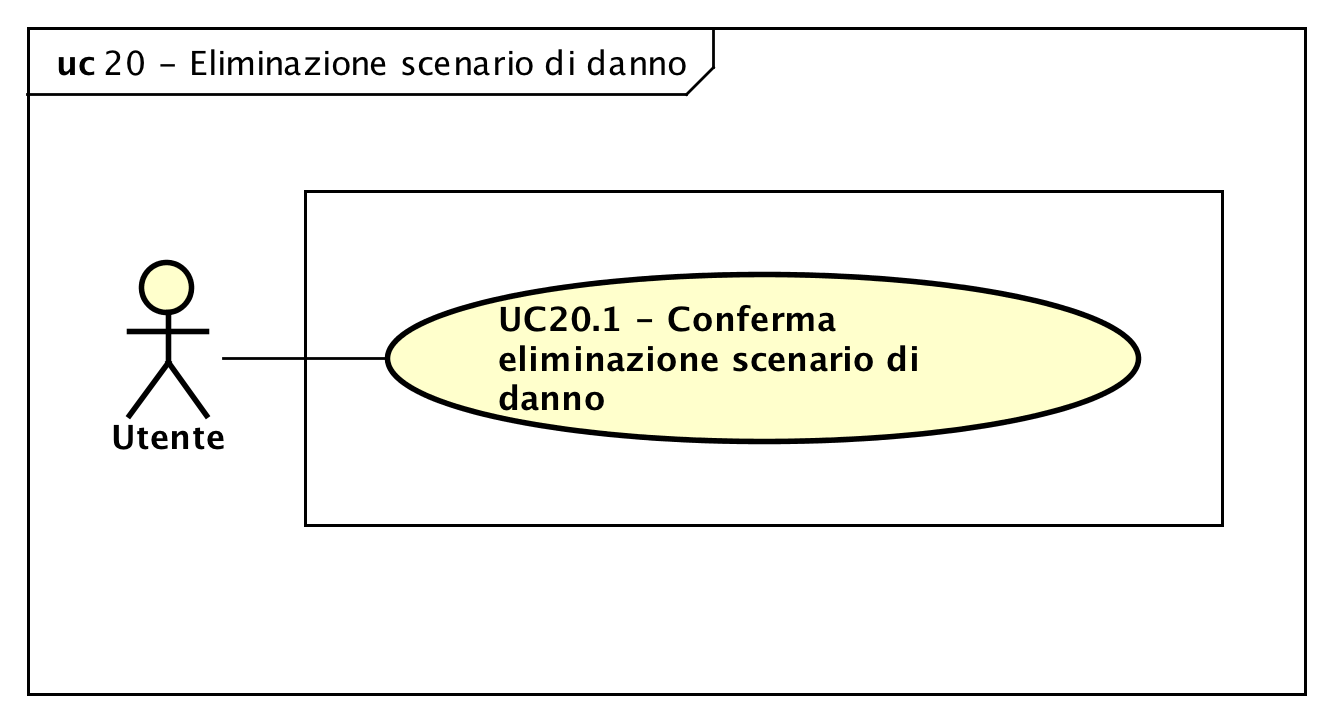
\includegraphics[scale=0.5]{{img/uc20}.png} 
	\caption{UC20 - Eliminazione scenario di danno}
\end{figure}
\def\arraystretch{1.5}
\rowcolors{2}{D}{P}
\begin{tabularx}{\textwidth}{l|p{0.7\textwidth}}
	\rowcolor{I} \multicolumn{2}{c}{\color{white}\textbf{UC20 - Eliminazione scenario di danno}} \\
	\toprule
	\endhead
	\textbf{Attori} & Utente\\
	\textbf{Descrizione} & l'utente elimina uno scenario\\
	\textbf{Pre-condizione} & l'utente ha aperto l'applicazione; è stato inserito almeno uno scenario; l'utente ha selezionato uno scenario\\
	\textbf{Post-condizione} & lo scenario è stato eliminato; l'utente visualizza un messaggio che comunica la corretta esecuzione dell'operazione;  l'area informativa viene impostata sulla visualizzazione di default;  la posizione e il livello di ingrandimento della mappa rimangono invariati\\
	\textbf{Scenario principale} & \vspace{-1.2em}\begin{enumerate}[leftmargin=*,noitemsep,nosep]
		\item \nameref{sssec:UC20.1}.
	\end{enumerate}\\
	\textbf{Estensioni} & \vspace{-1.2em}\begin{itemize}[leftmargin=*,noitemsep,nosep]
		\item \nameref{sssec:UC41}: l'utente interrompe volontariamente l'eliminazione dello
		scenario di danno
	\end{itemize}\\
	%\textbf{Generalizzazioni} &  \\
	\bottomrule
\end{tabularx}
\subsection{UC20.1 - Conferma eliminazione scenario di danno} 
\label{sssec:UC20.1} 
\def\arraystretch{1.5}
\rowcolors{2}{D}{P}
\begin{tabularx}{\textwidth}{l|p{0.7\textwidth}}
	\rowcolor{I} \multicolumn{2}{c}{\color{white}\textbf{UC20.1 - Conferma eliminazione scenario di danno}} \\
	\toprule
	\endhead
	\textbf{Attori} & Utente\\
	\textbf{Descrizione} & l'utente conferma l'eliminazione dello scenario di danno\\
	\textbf{Pre-condizione} & il sistema offre la possibilità di confermare l'eliminazione dello scenario di danno\\
	\textbf{Post-condizione} & lo scenario è stato eliminato; l'utente visualizza un messaggio che comunica la corretta esecuzione dell'operazione;  l'area informativa viene impostata sulla visualizzazione di default;  la posizione e il livello di ingrandimento della mappa rimangono invariati\\
		\textbf{Scenario principale} & \vspace{-1.2em}\begin{enumerate}[leftmargin=*,noitemsep,nosep]
		\item \nameref{sssec:UC20.1}.
	\end{enumerate}\\
	%\textbf{Generalizzazioni} &  \\
	\bottomrule
\end{tabularx}
\subsection{UC21 - Avvio analisi di danno} 
\label{sssec:UC21} 
\def\arraystretch{1.5}
\rowcolors{2}{D}{P}
\begin{tabularx}{\textwidth}{l|p{0.7\textwidth}}
	\rowcolor{I} \multicolumn{2}{c}{\color{white}\textbf{UC21 - Avvio analisi di danno}} \\
	\toprule
	\endhead
	\textbf{Attori} & Utente\\
	\textbf{Descrizione} & l'utente avvia l'analisi di danno\\
	\textbf{Pre-condizione} & l'utente ha aperto l'applicazione\\
	\textbf{Post-condizione} & la richiesta di processo dell'analisi di danno è stata inviata al server di calcolo; l'utente visualizza un messaggio riguardante l'invio della richiesta\\
	\textbf{Scenario principale} & \vspace{-1.2em}\begin{enumerate}[leftmargin=*,noitemsep,nosep]
		\item \nameref{sssec:UC21}.
	\end{enumerate}\\
	%\textbf{Generalizzazioni} &  \\
	\bottomrule
\end{tabularx}
\subsection{UC22 - Visualizzazione risultato analisi di danno su mappa} 
\label{sssec:UC22} 
\def\arraystretch{1.5}
\rowcolors{2}{D}{P}
\begin{tabularx}{\textwidth}{l|p{0.7\textwidth}}
	\rowcolor{I} \multicolumn{2}{c}{\color{white}\textbf{UC22 - Visualizzazione risultato analisi di danno su mappa}} \\
	\toprule
	\endhead
	\textbf{Attori} & Utente\\
	\textbf{Descrizione} & l'utente visualizza il risultato dell'analisi di danno sulla mappa\\
	\textbf{Pre-condizione} & l'utente ha aperto l'applicazione; i risultati dell'analisi di danno sono stati ricevuti\\
	\textbf{Post-condizione} & viene visualizzata su mappa il risultato dell'analisi di danno\\
	\textbf{Scenario principale} & \vspace{-1.2em}\begin{enumerate}[leftmargin=*,noitemsep,nosep]
		\item \nameref{sssec:UC22}.
	\end{enumerate}\\
	%\textbf{Generalizzazioni} &  \\
	\bottomrule
\end{tabularx}
\subsection{UC23 - Chiusura visualizzazione risultato analisi di danno su mappa} 
\label{sssec:UC23} 
\def\arraystretch{1.5}
\rowcolors{2}{D}{P}
\begin{tabularx}{\textwidth}{l|p{0.7\textwidth}}
	\rowcolor{I} \multicolumn{2}{c}{\color{white}\textbf{UC23 - Chiusura visualizzazione risultato analisi di danno su mappa}} \\
	\toprule
	\endhead
	\textbf{Attori} & Utente\\
	\textbf{Descrizione} & l'utente chiude la visualizzazione dell'analisi di danno sulla mappa\\
	\textbf{Pre-condizione} & l'utente ha aperto l'applicazione; i risultati dell'analisi di danno sono visualizzati\\
	\textbf{Post-condizione} & i risultati dell'analisi di danno non sono più visualizzati sulla mappa;  l'area informativa viene impostata sulla visualizzazione di default; la posizione e il livello di ingrandimento della mappa rimangono invariati\\
	\textbf{Scenario principale} & \vspace{-1.2em}\begin{enumerate}[leftmargin=*,noitemsep,nosep]
		\item \nameref{sssec:UC23}.
	\end{enumerate}\\
	%\textbf{Generalizzazioni} &  \\
	\bottomrule
\end{tabularx}
\subsection{UC24 - Interazione con la mappa} 
\label{sssec:UC24} 
\begin{figure}[H] 
	\centering 
	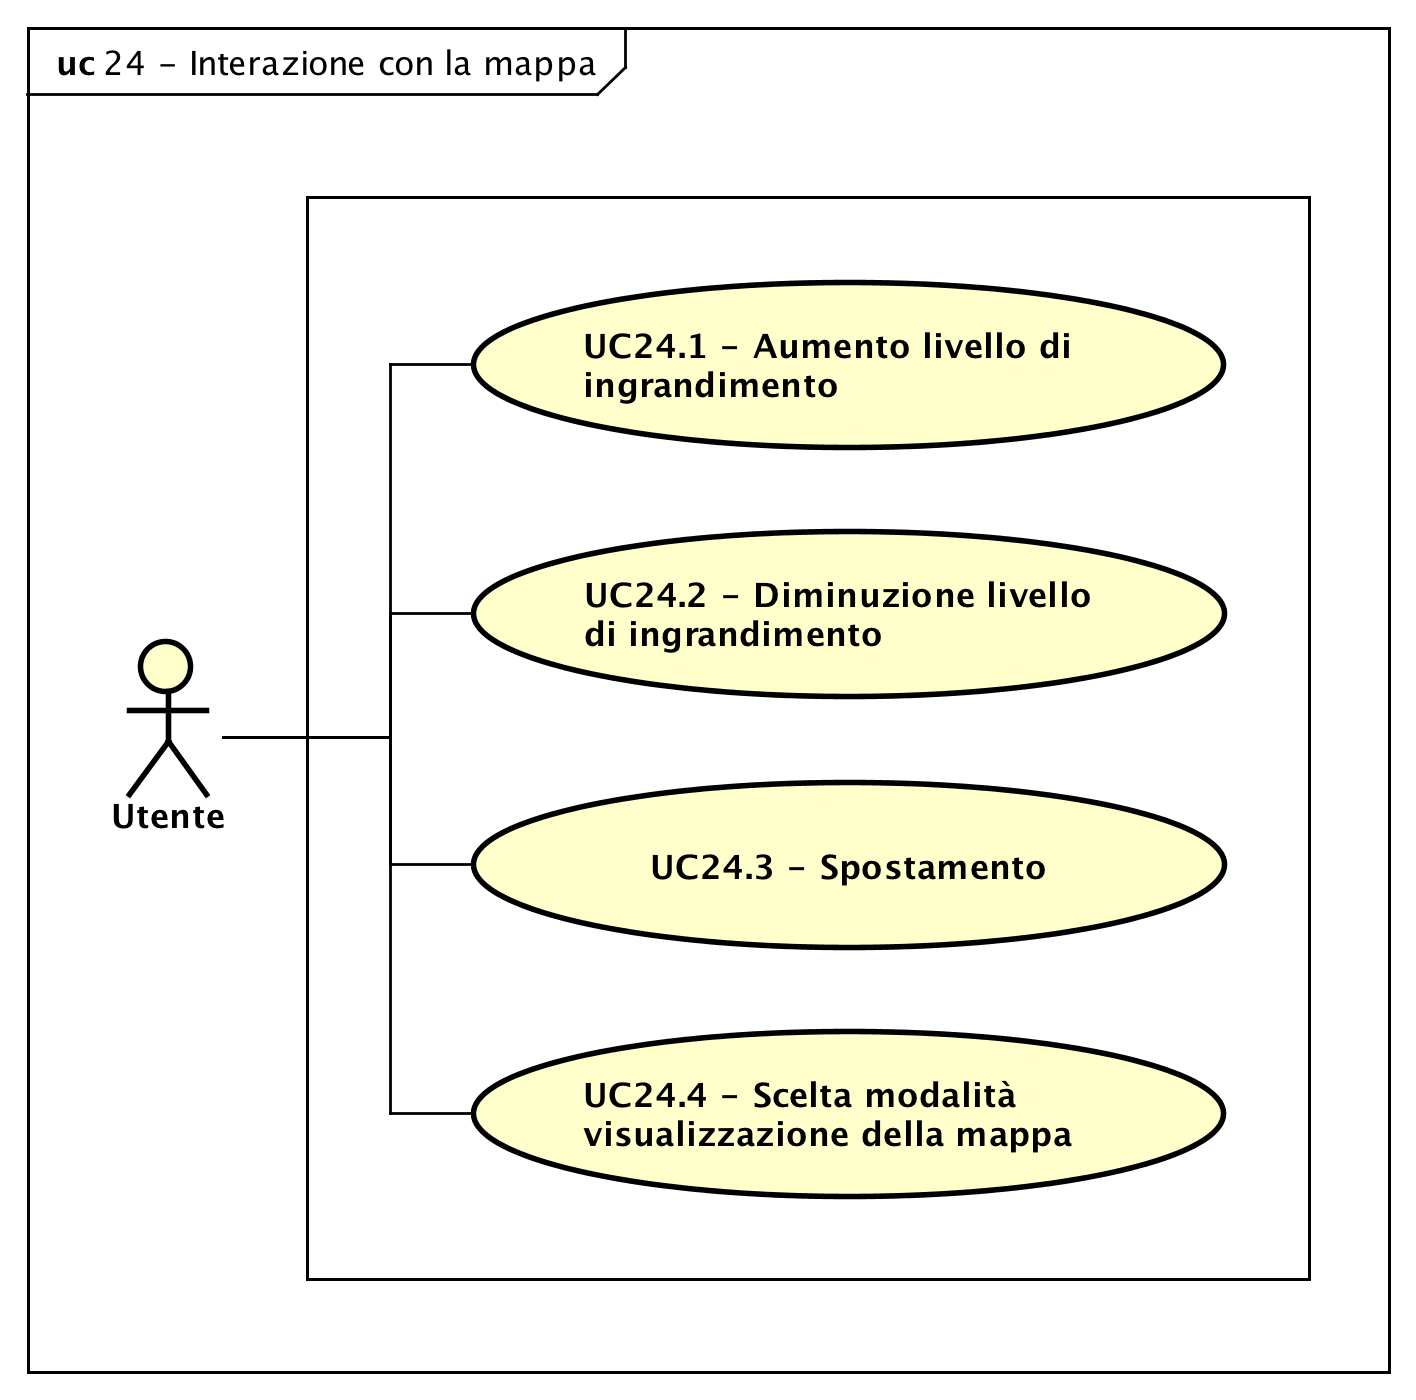
\includegraphics[scale=0.5]{{img/uc24}.png} 
	\caption{UC24 - Interazione con la mappa}
\end{figure}
\def\arraystretch{1.5}
\rowcolors{2}{D}{P}
\begin{tabularx}{\textwidth}{l|p{0.7\textwidth}}
	\rowcolor{I} \multicolumn{2}{c}{\color{white}\textbf{UC24 - Interazione con la mappa}} \\
	\toprule
	\endhead
	\textbf{Attori} & Utente\\
	\textbf{Descrizione} & l'utente interagisce con la mappa\\
	\textbf{Pre-condizione} & l'utente ha aperto l'applicazione\\
	\textbf{Post-condizione} & la mappa ha subito un'interazione; la visualizzazione della mappa è cambiata\\
	\textbf{Scenario principale} & \vspace{-1.2em}\begin{enumerate}[leftmargin=*,noitemsep,nosep]
		\item \nameref{sssec:UC24.1};
		\item \nameref{sssec:UC24.2};
		\item \nameref{sssec:UC24.3};
		\item \nameref{sssec:UC24.4}.
	\end{enumerate}\\
	%\textbf{Generalizzazioni} &  \\
	\bottomrule
\end{tabularx}
\subsection{UC24.1 - Aumento livello di ingrandimento} 
\label{sssec:UC24.1} 
\def\arraystretch{1.5}
\rowcolors{2}{D}{P}
\begin{tabularx}{\textwidth}{l|p{0.7\textwidth}}
	\rowcolor{I} \multicolumn{2}{c}{\color{white}\textbf{UC24.1 - Aumento livello di ingrandimento}} \\
	\toprule
	\endhead
	\textbf{Attori} & Utente\\
	\textbf{Descrizione} & l'utente aumenta il livello di ingrandimento della mappa\\
	\textbf{Pre-condizione} & l'utente ha aperto l'applicazione; il livello di zoom della mappa può essere aumentato\\
	\textbf{Post-condizione} & il livello di zoom della mappa è stato aumentato\\
	\textbf{Scenario principale} & \vspace{-1.2em}\begin{enumerate}[leftmargin=*,noitemsep,nosep]
		\item \nameref{sssec:UC24.1}.
	\end{enumerate}\\
	%\textbf{Generalizzazioni} &  \\
	\bottomrule
\end{tabularx}
\subsection{UC24.2 - Diminuzione livello di ingrandimento} 
\label{sssec:UC24.2} 
\def\arraystretch{1.5}
\rowcolors{2}{D}{P}
\begin{tabularx}{\textwidth}{l|p{0.7\textwidth}}
	\rowcolor{I} \multicolumn{2}{c}{\color{white}\textbf{UC24.2 - Diminuzione livello di ingrandimento}} \\
	\toprule
	\endhead
	\textbf{Attori} & Utente\\
	\textbf{Descrizione} & l'utente diminuisce il livello di ingrandimento della mappa\\
	\textbf{Pre-condizione} & l'utente ha aperto l'applicazione; il livello di zoom della mappa può essere diminuito\\
	\textbf{Post-condizione} & il livello di zoom della mappa è stato diminuito\\
	\textbf{Scenario principale} & \vspace{-1.2em}\begin{enumerate}[leftmargin=*,noitemsep,nosep]
		\item \nameref{sssec:UC24.2}.
	\end{enumerate}\\
	%\textbf{Generalizzazioni} &  \\
	\bottomrule
\end{tabularx}
\subsection{UC24.3 - Spostamento} 
\label{sssec:UC24.3} 
\def\arraystretch{1.5}
\rowcolors{2}{D}{P}
\begin{tabularx}{\textwidth}{l|p{0.7\textwidth}}
	\rowcolor{I} \multicolumn{2}{c}{\color{white}\textbf{UC24.3 - Spostamento}} \\
	\toprule
	\endhead
	\textbf{Attori} & Utente\\
	\textbf{Descrizione} & l'utente sposta la visualizzazione della mappa\\
	\textbf{Pre-condizione} & l'utente ha aperto l'applicazione; la visualizzazione della mappa può essere spostata\\
	\textbf{Post-condizione} & la visualizzazione della mappa è stata spostata\\
	\textbf{Scenario principale} & \vspace{-1.2em}\begin{enumerate}[leftmargin=*,noitemsep,nosep]
		\item \nameref{sssec:UC24.3}.
	\end{enumerate}\\
	%\textbf{Generalizzazioni} &  \\
	\bottomrule
\end{tabularx}
\subsection{UC24.4 - Scelta modalità visualizzazione della mappa} 
\label{sssec:UC24.4} 
\def\arraystretch{1.5}
\rowcolors{2}{D}{P}
\begin{tabularx}{\textwidth}{l|p{0.7\textwidth}}
	\rowcolor{I} \multicolumn{2}{c}{\color{white}\textbf{UC24.4 - Scelta modalità visualizzazione della mappa}} \\
	\toprule
	\endhead
	\textbf{Attori} & Utente\\
	\textbf{Descrizione} & l'utente sceglie la modalità di visualizzazione della mappa\\
	\textbf{Pre-condizione} & l'utente ha aperto l'applicazione; la modalità di visualizzazione della mappa può essere scelta\\
	\textbf{Post-condizione} & la modalità di visualizzazione della mappa è stata scelta; la mappa cambia di conseguenza\\
	\textbf{Scenario principale} & \vspace{-1.2em}\begin{enumerate}[leftmargin=*,noitemsep,nosep]
		\item \nameref{sssec:UC24.4}.
	\end{enumerate}\\
	%\textbf{Generalizzazioni} &  \\
	\bottomrule
\end{tabularx}
\subsection{UC25 - Fruizione tutorial} 
\label{sssec:UC25} 
\def\arraystretch{1.5}
\rowcolors{2}{D}{P}
\begin{tabularx}{\textwidth}{l|p{0.7\textwidth}}
	\rowcolor{I} \multicolumn{2}{c}{\color{white}\textbf{UC25 - Avvio tutorial}} \\
	\toprule
	\endhead
	\textbf{Attori} & Utente\\
	\textbf{Descrizione} & l'utente avvia il tutorial ed esegue tutte le operazioni che l'applicazione offre in modo guidato\\
	\textbf{Pre-condizione} & l'utente ha aperto l'applicazione; il tutorial può essere avviato\\
	\textbf{Post-condizione} & il tutorial è stato completato; l'area informativa viene impostata alla visualizzazione di default; durante l'esecuzione del tutorial vengono visualizzate informazioni relative alle varie operazioni che l'utente può eseguire; l'utente può eseguire tutte le operazioni permesse dal sistema in modo guidato\\
	\textbf{Scenario principale} & \vspace{-1.2em}\begin{enumerate}[leftmargin=*,noitemsep,nosep]
		\item \nameref{sssec:UC25}.
	\end{enumerate}\\
	\textbf{Estensioni} & \vspace{-1.2em}\begin{itemize}[leftmargin=*,noitemsep,nosep]
	\item \nameref{sssec:UC46}: l'utente interrompe volontariamente
	la fruizione del tutorial
\end{itemize}\\
	%\textbf{Generalizzazioni} &  \\
	\bottomrule
\end{tabularx}
\subsection{UC26 - Fruizione assistente vocale} 
\label{sssec:UC26} 
\def\arraystretch{1.5}
\rowcolors{2}{D}{P}
\begin{tabularx}{\textwidth}{l|p{0.7\textwidth}}
	\rowcolor{I} \multicolumn{2}{c}{\color{white}\textbf{UC26 - Avvio assistente vocale}} \\
	\toprule
	\endhead
	\textbf{Attori} & Utente\\
	\textbf{Descrizione} & l'utente avvia l'assistente vocale ed esegue le operazioni con l'ausilio della voce\\
	\textbf{Pre-condizione} & l'utente ha aperto l'applicazione; l'assistente vocale può essere avviato\\
	\textbf{Post-condizione} & l'assistente vocale ha effettuato l'operazione chiesta dall'utente; l'area informativa viene impostata alla visualizzazione di default; durante l'esecuzione dell'assistente vocale l'utente può eseguire tutte le operazioni permesse dal sistema con l'ausilio della voce\\
	\textbf{Scenario principale} & \vspace{-1.2em}\begin{enumerate}[leftmargin=*,noitemsep,nosep]
		\item \nameref{sssec:UC26}.
	\end{enumerate}\\
	%\textbf{Generalizzazioni} &  \\
	\bottomrule
\end{tabularx}
\subsection{UC27 - Ritorno visuale asset selezionato} 
\label{sssec:UC27} 
\def\arraystretch{1.5}
\rowcolors{2}{D}{P}
\begin{tabularx}{\textwidth}{l|p{0.7\textwidth}}
	\rowcolor{I} \multicolumn{2}{c}{\color{white}\textbf{UC27 - Ritorno visuale asset selezionato}} \\
	\toprule
	\endhead
	\textbf{Attori} & Utente\\
	\textbf{Descrizione} & l'utente viene riportato alla visualizzazione dell'asset selezionato\\
	\textbf{Pre-condizione} & l'utente ha visualizzato le informazioni di un asset\\
	\textbf{Post-condizione} & il sistema riporta la visualizzazione della mappa in modo tale da visualizzare i nodi all'interno dell'asset selezionato\\
	\textbf{Scenario principale} & \vspace{-1.2em}\begin{enumerate}[leftmargin=*,noitemsep,nosep]
		\item \nameref{sssec:UC27}.
	\end{enumerate}\\
	%\textbf{Generalizzazioni} &  \\
	\bottomrule
\end{tabularx}
\subsection{UC28 - Ritorno visuale nodo selezionato} 
\label{sssec:UC28} 
\def\arraystretch{1.5}
\rowcolors{2}{D}{P}
\begin{tabularx}{\textwidth}{l|p{0.7\textwidth}}
	\rowcolor{I} \multicolumn{2}{c}{\color{white}\textbf{UC28 - Ritorno visuale nodo selezionato}} \\
	\toprule
	\endhead
	\textbf{Attori} & Utente\\
	\textbf{Descrizione} & l'utente viene riportato alla visualizzazione del nodo selezionato\\
	\textbf{Pre-condizione} & l'utente ha visualizzato le informazioni di un nodo\\
	\textbf{Post-condizione} & il sistema riporta la visualizzazione della mappa in modo tale da visualizzare il nodo selezionato\\
	\textbf{Scenario principale} & \vspace{-1.2em}\begin{enumerate}[leftmargin=*,noitemsep,nosep]
		\item \nameref{sssec:UC28}.
	\end{enumerate}\\
	%\textbf{Generalizzazioni} &  \\
	\bottomrule
\end{tabularx}
\subsection{UC29 - Ritorno visuale arco selezionato} 
\label{sssec:UC29} 
\def\arraystretch{1.5}
\rowcolors{2}{D}{P}
\begin{tabularx}{\textwidth}{l|p{0.7\textwidth}}
	\rowcolor{I} \multicolumn{2}{c}{\color{white}\textbf{UC29 - Ritorno visuale arco selezionato}} \\
	\toprule
	\endhead
	\textbf{Attori} & Utente\\
	\textbf{Descrizione} & l'utente viene riportato alla visualizzazione dell'arco selezionato\\
	\textbf{Pre-condizione} & l'utente ha visualizzato le informazioni di un arco\\
	\textbf{Post-condizione} & il sistema riporta la visualizzazione della mappa in modo tale da visualizzare l'arco selezionato\\
	\textbf{Scenario principale} & \vspace{-1.2em}\begin{enumerate}[leftmargin=*,noitemsep,nosep]
		\item \nameref{sssec:UC29}.
	\end{enumerate}\\
	%\textbf{Generalizzazioni} &  \\
	\bottomrule
\end{tabularx}

\subsection{UC30 - Interruzione aggiunta asset} 
\label{sssec:UC30} 
\def\arraystretch{1.5}
\rowcolors{2}{D}{P}
\begin{tabularx}{\textwidth}{l|p{0.7\textwidth}}
	\rowcolor{I} \multicolumn{2}{c}{\color{white}\textbf{UC30 - Interruzione aggiunta asset}} \\
	\toprule
	\endhead
	\textbf{Attori} & Utente\\
	\textbf{Descrizione} & l'utente interrompe l'aggiunta dell'asset\\
	\textbf{Pre-condizione} & il sistema offre la possibilità di aggiungere un asset\\
	\textbf{Post-condizione} & nessun asset è stato aggiunto; l'area informativa viene impostata sulla visualizzazione di default; la posizione e il livello di ingrandimento della mappa rimangono invariati\\
	\textbf{Scenario principale} & \vspace{-1.2em}\begin{enumerate}[leftmargin=*,noitemsep,nosep]
		\item \nameref{sssec:UC30}.
	\end{enumerate}\\
	%\textbf{Generalizzazioni} &  \\
	\bottomrule
\end{tabularx}
\subsection{UC31 - Interruzione modifica asset} 
\label{sssec:UC31} 
\def\arraystretch{1.5}
\rowcolors{2}{D}{P}
\begin{tabularx}{\textwidth}{l|p{0.7\textwidth}}
	\rowcolor{I} \multicolumn{2}{c}{\color{white}\textbf{UC31 - Interruzione modifica asset}} \\
	\toprule
	\endhead
	\textbf{Attori} & Utente\\
	\textbf{Descrizione} & l'utente interrompe la modifica dell'asset\\
	\textbf{Pre-condizione} & il sistema offre la possibilità di modificare un asset\\
	\textbf{Post-condizione} & l'asset non è stato modificato; l'area informativa viene impostata sulla visualizzazione di default; la posizione e il livello di ingrandimento della mappa rimangono invariati\\
	\textbf{Scenario principale} & \vspace{-1.2em}\begin{enumerate}[leftmargin=*,noitemsep,nosep]
		\item \nameref{sssec:UC31}.
	\end{enumerate}\\
	%\textbf{Generalizzazioni} &  \\
	\bottomrule
\end{tabularx}
\subsection{UC32 - Interruzione eliminazione asset} 
\label{sssec:UC32} 
\def\arraystretch{1.5}
\rowcolors{2}{D}{P}
\begin{tabularx}{\textwidth}{l|p{0.7\textwidth}}
	\rowcolor{I} \multicolumn{2}{c}{\color{white}\textbf{UC32 - Interruzione eliminazione asset}} \\
	\toprule
	\endhead
	\textbf{Attori} & Utente\\
	\textbf{Descrizione} & l'utente interrompe l'eliminazione dell'asset\\
	\textbf{Pre-condizione} & il sistema offre la possibilità di confermare l'eliminazione dell'asset\\
	\textbf{Post-condizione} & l'asset non è stato eliminato; l'area informativa viene impostata sulla visualizzazione di default; la posizione e il livello di ingrandimento della mappa rimangono invariati\\
	\textbf{Scenario principale} & \vspace{-1.2em}\begin{enumerate}[leftmargin=*,noitemsep,nosep]
		\item \nameref{sssec:UC32}.
	\end{enumerate}\\
	%\textbf{Generalizzazioni} &  \\
	\bottomrule
\end{tabularx}
\subsection{UC33 - Interruzione aggiunta nodo} 
\label{sssec:UC33} 
\def\arraystretch{1.5}
\rowcolors{2}{D}{P}
\begin{tabularx}{\textwidth}{l|p{0.7\textwidth}}
	\rowcolor{I} \multicolumn{2}{c}{\color{white}\textbf{UC33 - Interruzione aggiunta nodo}} \\
	\toprule
	\endhead
	\textbf{Attori} & Utente\\
	\textbf{Descrizione} & l'utente interrompe l'aggiunta di un nodo\\
	\textbf{Pre-condizione} & il sistema offre la possibilità di aggiungere un nodo\\
	\textbf{Post-condizione} & nessun nuovo nodo è stato aggiunto;  l'area informativa viene impostata sulla visualizzazione di default; la posizione e il livello di ingrandimento della mappa rimangono invariati\\
	\textbf{Scenario principale} & \vspace{-1.2em}\begin{enumerate}[leftmargin=*,noitemsep,nosep]
		\item \nameref{sssec:UC33}.
	\end{enumerate}\\
	%\textbf{Generalizzazioni} &  \\
	\bottomrule
\end{tabularx}
\subsection{UC34 - Interruzione modifica nodo} 
\label{sssec:UC34} 
\def\arraystretch{1.5}
\rowcolors{2}{D}{P}
\begin{tabularx}{\textwidth}{l|p{0.7\textwidth}}
	\rowcolor{I} \multicolumn{2}{c}{\color{white}\textbf{UC34 - Interruzione modifica nodo}} \\
	\toprule
	\endhead
	\textbf{Attori} & Utente\\
	\textbf{Descrizione} & l'utente interrompe la modifica del nodo\\
	\textbf{Pre-condizione} & il sistema offre la possibilità di modificare un nodo\\
	\textbf{Post-condizione} & il nodo non è stato modificato;  l'area informativa viene impostata sulla visualizzazione di default; la posizione e il livello di ingrandimento della mappa rimangono invariati\\
	\textbf{Scenario principale} & \vspace{-1.2em}\begin{enumerate}[leftmargin=*,noitemsep,nosep]
		\item \nameref{sssec:UC34}.
	\end{enumerate}\\
	%\textbf{Generalizzazioni} &  \\
	\bottomrule
\end{tabularx}
\subsection{UC35 - Interruzione eliminazione nodo} 
\label{sssec:UC35} 
\def\arraystretch{1.5}
\rowcolors{2}{D}{P}
\begin{tabularx}{\textwidth}{l|p{0.7\textwidth}}
	\rowcolor{I} \multicolumn{2}{c}{\color{white}\textbf{UC35 - Interruzione eliminazione nodo}} \\
	\toprule
	\endhead
	\textbf{Attori} & Utente\\
	\textbf{Descrizione} & l'utente interrompe l'eliminazione del nodo\\
	\textbf{Pre-condizione} & il sistema offre la possibilità di confermare l'eliminazione del nodo\\
	\textbf{Post-condizione} & il nodo non è stato eliminato e rimane visibile sulla mappa; l'area informativa viene impostata sulla visualizzazione di default;  la posizione e il livello di ingrandimento della mappa rimangono invariati\\
	\textbf{Scenario principale} & \vspace{-1.2em}\begin{enumerate}[leftmargin=*,noitemsep,nosep]
		\item \nameref{sssec:UC35}.
	\end{enumerate}\\
	%\textbf{Generalizzazioni} &  \\
	\bottomrule
\end{tabularx}
\subsection{UC36 - Interruzione aggiunta arco} 
\label{sssec:UC36} 
\def\arraystretch{1.5}
\rowcolors{2}{D}{P}
\begin{tabularx}{\textwidth}{l|p{0.7\textwidth}}
	\rowcolor{I} \multicolumn{2}{c}{\color{white}\textbf{UC36 - Interruzione aggiunta arco}} \\
	\toprule
	\endhead
	\textbf{Attori} & Utente\\
	\textbf{Descrizione} & l'utente interrompe l'aggiunta dell'arco\\
	\textbf{Pre-condizione} & il sistema offre la possibilità di aggiungere un arco\\
	\textbf{Post-condizione} & nessun arco è stato aggiunto; l'area informativa viene impostata sulla visualizzazione di default; la posizione e il livello di ingrandimento della mappa rimangono invariati\\
	\textbf{Scenario principale} & \vspace{-1.2em}\begin{enumerate}[leftmargin=*,noitemsep,nosep]
		\item \nameref{sssec:UC36}.
	\end{enumerate}\\
	%\textbf{Generalizzazioni} &  \\
	\bottomrule
\end{tabularx}
\subsection{UC37 - Interruzione modifica arco} 
\label{sssec:UC37} 
\def\arraystretch{1.5}
\rowcolors{2}{D}{P}
\begin{tabularx}{\textwidth}{l|p{0.7\textwidth}}
	\rowcolor{I} \multicolumn{2}{c}{\color{white}\textbf{UC37 - Interruzione modifica arco}} \\
	\toprule
	\endhead
	\textbf{Attori} & Utente\\
	\textbf{Descrizione} & l'utente interrompe la modifica dell'arco\\
	\textbf{Pre-condizione} & il sistema offre la possibilità di modificare un arco\\
	\textbf{Post-condizione} & l'arco non è stato modificato; l'area informativa viene impostata sulla visualizzazione di default; la posizione e il livello di ingrandimento della mappa rimangono invariati\\
	\textbf{Scenario principale} & \vspace{-1.2em}\begin{enumerate}[leftmargin=*,noitemsep,nosep]
		\item \nameref{sssec:UC37}.
	\end{enumerate}\\
	%\textbf{Generalizzazioni} &  \\
	\bottomrule
\end{tabularx}
\subsection{UC38 - Interruzione eliminazione arco} 
\label{sssec:UC38} 
\def\arraystretch{1.5}
\rowcolors{2}{D}{P}
\begin{tabularx}{\textwidth}{l|p{0.7\textwidth}}
	\rowcolor{I} \multicolumn{2}{c}{\color{white}\textbf{UC38 - Interruzione eliminazione arco}} \\
	\toprule
	\endhead
	\textbf{Attori} & Utente\\
	\textbf{Descrizione} & l'utente interrompe l'eliminazione dell'arco\\
	\textbf{Pre-condizione} & il sistema offre la possibilità di confermare l'eliminazione dell'arco\\
	\textbf{Post-condizione} & l'arco non è stato eliminato ed è ancora visibile sulla mappa; l'area informativa viene impostata sulla visualizzazione di default;  la posizione e il livello di ingrandimento della mappa rimangono invariati\\
	\textbf{Scenario principale} & \vspace{-1.2em}\begin{enumerate}[leftmargin=*,noitemsep,nosep]
		\item \nameref{sssec:UC38}.
	\end{enumerate}\\
	%\textbf{Generalizzazioni} &  \\
	\bottomrule
\end{tabularx}
\subsection{UC39 - Interruzione aggiunta scenario di danno} 
\label{sssec:UC39} 
\def\arraystretch{1.5}
\rowcolors{2}{D}{P}
\begin{tabularx}{\textwidth}{l|p{0.7\textwidth}}
	\rowcolor{I} \multicolumn{2}{c}{\color{white}\textbf{UC39 - Interruzione aggiunta scenario di danno}} \\
	\toprule
	\endhead
	\textbf{Attori} & Utente\\
	\textbf{Descrizione} & l'utente interrompe l'aggiunta dello scenario di danno\\
	\textbf{Pre-condizione} & il sistema offre la possibilità di aggiungere uno scenario di danno\\
	\textbf{Post-condizione} & nessuno scenario è stato aggiunto; l'area informativa viene impostata sulla visualizzazione di default; la posizione e il livello di ingrandimento della mappa rimangono invariati\\
	\textbf{Scenario principale} & \vspace{-1.2em}\begin{enumerate}[leftmargin=*,noitemsep,nosep]
		\item \nameref{sssec:UC39}: l’utente interrompe volontariamente l’aggiunta dello
		scenario di danno;
	\end{enumerate}\\
	%\textbf{Generalizzazioni} &  \\
	\bottomrule
\end{tabularx}

\subsection{UC40 - Interruzione modifica scenario} 
\label{sssec:UC40} 
\def\arraystretch{1.5}
\rowcolors{2}{D}{P}
\begin{tabularx}{\textwidth}{l|p{0.7\textwidth}}
	\rowcolor{I} \multicolumn{2}{c}{\color{white}\textbf{UC40 - Interruzione modifica scenario}} \\
	\toprule
	\endhead
	\textbf{Attori} & Utente\\
	\textbf{Descrizione} & l'utente interrompe la modifica dello scenario\\
	\textbf{Pre-condizione} & il sistema offre la possibilità di modificare lo scenario\\
	\textbf{Post-condizione} & lo scenario non è stato modificato;  l'area informativa viene impostata sulla visualizzazione di default; la posizione e il livello di ingrandimento della mappa rimangono invariati\\
	\textbf{Scenario principale} & \vspace{-1.2em}\begin{enumerate}[leftmargin=*,noitemsep,nosep]
		\item \nameref{sssec:UC40}.
	\end{enumerate}\\
	%\textbf{Generalizzazioni} &  \\
	\bottomrule
\end{tabularx}
\subsection{UC41 - Interruzione eliminazione scenario di danno} 
\label{sssec:UC41} 
\def\arraystretch{1.5}
\rowcolors{2}{D}{P}
\begin{tabularx}{\textwidth}{l|p{0.7\textwidth}}
	\rowcolor{I} \multicolumn{2}{c}{\color{white}\textbf{UC41 - Interruzione eliminazione scenario di danno}} \\
	\toprule
	\endhead
	\textbf{Attori} & Utente\\
	\textbf{Descrizione} & l'utente interrompe l'eliminazione dello scenario di danno\\
	\textbf{Pre-condizione} & il sistema offre la possibilità di confermare l'eliminazione dello scenario di danno\\
	\textbf{Post-condizione} & lo scenario di danno non è stato eliminato;  l'area informativa viene impostata sulla visualizzazione di default;  la posizione e il livello di ingrandimento della mappa rimangono invariati
	\\
	\textbf{Scenario principale} & \vspace{-1.2em}\begin{enumerate}[leftmargin=*,noitemsep,nosep]
		\item \nameref{sssec:UC41}.
	\end{enumerate}\\
	%\textbf{Generalizzazioni} &  \\
	\bottomrule
\end{tabularx}
\subsection{UC42 - Selezione scenario di danno per analisi di danno} 
\label{sssec:UC42} 
\def\arraystretch{1.5}
\rowcolors{2}{D}{P}
\begin{tabularx}{\textwidth}{l|p{0.7\textwidth}}
	\rowcolor{I} \multicolumn{2}{c}{\color{white}\textbf{UC42 - Selezione scenario di danno per analisi di danno}} \\
	\toprule
	\endhead
	\textbf{Attori} & Utente\\
	\textbf{Descrizione} & l'utente aggiunge uno scenario di danno alla lista di quelli da prendere in considerazione per la successiva analisi\\
	\textbf{Pre-condizione} & è stato inserito almeno uno scenario di danno\\
	\textbf{Post-condizione} & lo scenario di dannno è stato aggiunto alla lista di quelli da prendere in considerazione per la successiva analisi; l'utente visualizza che lo scenario è stato selezionato \\
	\textbf{Scenario principale} & \vspace{-1.2em}\begin{enumerate}[leftmargin=*,noitemsep,nosep]
		\item \nameref{sssec:UC42}.
	\end{enumerate}\\
	%\textbf{Generalizzazioni} &  \\
	\bottomrule
\end{tabularx}
\subsection{UC43 - Deselezione scenario di danno per analisi di danno} 
\label{sssec:UC43} 
\def\arraystretch{1.5}
\rowcolors{2}{D}{P}
\begin{tabularx}{\textwidth}{l|p{0.7\textwidth}}
	\rowcolor{I} \multicolumn{2}{c}{\color{white}\textbf{UC43 - Deselezione scenario di danno per analisi di danno}} \\
	\toprule
	\endhead
	\textbf{Attori} & Utente\\
	\textbf{Descrizione} & l'utente rimuove uno scenario di danno dalla lista di quelli da prendere in considerazione per la successiva analisi\\
	\textbf{Pre-condizione} & è stato inserito almeno uno scenario di danno; è stato selezionato almeno uno scenario di danno per l'analisi di danno\\
	\textbf{Post-condizione} & lo scenario di dannno è stato rimosso alla lista di quelli da prendere in considerazione per la successiva analisi; l'utente visualizza che lo scenario è stato deselezionato \\
	\textbf{Scenario principale} & \vspace{-1.2em}\begin{enumerate}[leftmargin=*,noitemsep,nosep]
		\item \nameref{sssec:UC43}.
	\end{enumerate}\\
	%\textbf{Generalizzazioni} &  \\
	\bottomrule
\end{tabularx}
\subsection{UC44 - Eliminazione analisi di danno} 
\label{sssec:UC44} 
\begin{figure}[H] 
	\centering 
	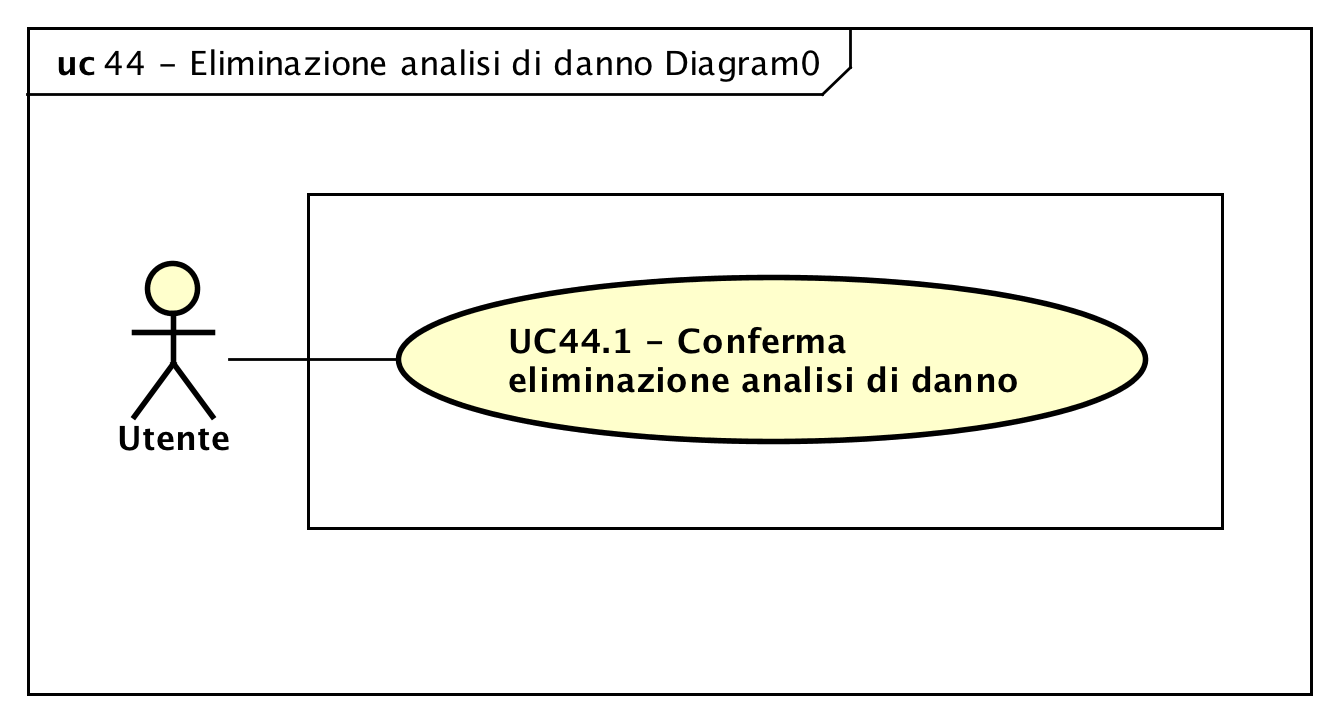
\includegraphics[scale=0.5]{{img/uc44}.png} 
	\caption{UC44 - Eliminazione analisi di danno}
\end{figure}
\def\arraystretch{1.5}
\rowcolors{2}{D}{P}
\begin{tabularx}{\textwidth}{l|p{0.7\textwidth}}
	\rowcolor{I} \multicolumn{2}{c}{\color{white}\textbf{UC44 - Eliminazione analisi di danno}} \\
	\toprule
	\endhead
	\textbf{Attori} & Utente\\
	\textbf{Descrizione} & l'utente elimina un analisi di danno precedentemente eseguita\\
	\textbf{Pre-condizione} & è stata calcolata almeno un'analisi di danno; è stata selezionata un'analisi di danno\\
	\textbf{Post-condizione} & l'analisi di danno è stata eliminata; l'utente visualizza un messaggio che comunica la corretta esecuzione dell'operazione;  l'area informativa viene impostata sulla visualizzazione di default;  la posizione e il livello di ingrandimento della mappa rimangono invariati\\
	\textbf{Estensioni} & \vspace{-1.2em}\begin{itemize}[leftmargin=*,noitemsep,nosep]
		\item \nameref{sssec:UC45}: l'utente interrompe volontariamente
		l'eliminazione dell'analisi di danno
	\end{itemize}\\
	%\textbf{Generalizzazioni} &  \\
	\bottomrule
\end{tabularx}
\subsection{UC44.1 - Conferma eliminazione analisi di danno} 
\label{sssec:UC44.1} 
\def\arraystretch{1.5}
\rowcolors{2}{D}{P}
\begin{tabularx}{\textwidth}{l|p{0.7\textwidth}}
	\rowcolor{I} \multicolumn{2}{c}{\color{white}\textbf{UC44.1 - Conferma eliminazione analisi di danno}} \\
	\toprule
	\endhead
	\textbf{Attori} & Utente\\
	\textbf{Descrizione} & l'utente conferma l'eliminazione dell'analisi di danno\\
	\textbf{Pre-condizione} & il sistema offre la possibilità di confermare l'eliminazione dell'analisi di danno\\
	\textbf{Post-condizione} & l'analisi di danno è stata eliminata; l'utente visualizza un messaggio che comunica la corretta esecuzione dell'operazione;  l'area informativa viene impostata sulla visualizzazione di default;  la posizione e il livello di ingrandimento della mappa rimangono invariati\\
	\textbf{Scenario principale} & \vspace{-1.2em}\begin{enumerate}[leftmargin=*,noitemsep,nosep]
		\item \nameref{sssec:UC44.1}.
	\end{enumerate}\\
	%\textbf{Generalizzazioni} &  \\
	\bottomrule
\end{tabularx}
\subsection{UC45 - Interruzione eliminazione analisi di danno} 
\label{sssec:UC45} 
\def\arraystretch{1.5}
\rowcolors{2}{D}{P}
\begin{tabularx}{\textwidth}{l|p{0.7\textwidth}}
	\rowcolor{I} \multicolumn{2}{c}{\color{white}\textbf{UC45 - Interruzione eliminazione analisi di danno}} \\
	\toprule
	\endhead
	\textbf{Attori} & Utente\\
	\textbf{Descrizione} & l'utente interrompe l'eliminazione dell'analisi di danno\\
	\textbf{Pre-condizione} & il sistema offre la possibilità di confermare l'eliminazione dell'analisi di danno\\
	\textbf{Post-condizione} & l'analisi di danno non è stata eliminata; l'area informativa viene impostata sulla visualizzazione di default; la posizione e il livello di ingrandimento della mappa rimangono invariati\\
	\textbf{Scenario principale} & \vspace{-1.2em}\begin{enumerate}[leftmargin=*,noitemsep,nosep]
		\item \nameref{sssec:UC45}.
	\end{enumerate}\\
	%\textbf{Generalizzazioni} &  \\
	\bottomrule
\end{tabularx}

\subsection{UC46 - Interruzione fruizione tutorial} 
\label{sssec:UC46} 
\def\arraystretch{1.5}
\rowcolors{2}{D}{P}
\begin{tabularx}{\textwidth}{l|p{0.7\textwidth}}
	\rowcolor{I} \multicolumn{2}{c}{\color{white}\textbf{UC46 - Interruzione fruizione tutorial}} \\
	\toprule
	\endhead
	\textbf{Attori} & Utente\\
	\textbf{Descrizione} & L'utente interrompe la fruizione del tutorial\\
	\textbf{Pre-condizione} & il tutorial sta eseguendo\\
	\textbf{Post-condizione} & l'utente ha interrotto la fruizione del tutorial; gli effetti delle operazioni eseguite all'interno del tutorial non vengono annullati; l'area informativa viene impostata alla visualizzazione di default\\
	\textbf{Scenario principale} & \vspace{-1.2em}\begin{enumerate}[leftmargin=*,noitemsep,nosep]
		\item \nameref{sssec:UC46}.
	\end{enumerate}\\
	%\textbf{Generalizzazioni} &  \\
	\bottomrule
\end{tabularx}
\subsection{UC47 - Interruzione fruizione assistente vocale} 
\label{sssec:UC47} 
\def\arraystretch{1.5}
\rowcolors{2}{D}{P}
\begin{tabularx}{\textwidth}{l|p{0.7\textwidth}}
	\rowcolor{I} \multicolumn{2}{c}{\color{white}\textbf{UC47 - Interruzione fruizione assistente vocale}} \\
	\toprule
	\endhead
	\textbf{Attori} & Utente\\
	\textbf{Descrizione} & L'utente interrompe la fruizione dell'assistente vocale\\
	\textbf{Pre-condizione} & l'assistente vocale sta eseguendo\\
	\textbf{Post-condizione} & l'utente ha interrotto la fruizione del tutorial; nessuna operazione è stata eseguita dall'assistente vocale; l'area informativa viene impostata alla visualizzazione di default\\
	\textbf{Scenario principale} & \vspace{-1.2em}\begin{enumerate}[leftmargin=*,noitemsep,nosep]
		\item \nameref{sssec:UC47}.
	\end{enumerate}\\
	%\textbf{Generalizzazioni} &  \\
	\bottomrule
\end{tabularx}

	\section{Requisiti}
\subsection{Classificazione dei requisiti}
I requisiti sono classificati secondo la seguente notazione:
\begin{center}
	R[Importanza][Tipologia][Codice]
\end{center}
dove:
\begin{itemize}
	\item \textbf{importanza:} può assumere questi valori:
	\begin{itemize}
		\item \textbf{O:} indica un requisito obbligatorio;
		\item \textbf{D:} indica un requisito desiderabile;
		\item \textbf{F:} indica un requisito opzionale (facoltativo).
	\end{itemize}
	\item \textbf{tipologia:} può assumere questi valori:
	\begin{itemize}
		\item \textbf{F:} indica un requisito funzionale;
		\item \textbf{Q:} indica un requisito di qualità;
		\item \textbf{P:} indica un requisito prestazionale;
		\item \textbf{V:} indica un requisito di vincolo.
	\end{itemize}
	\item \textbf{codice:} codice numerico che identifica il requisito, deve essere univoco ed indicato in forma gerarchica, da sinistra a destra, nella notazione X.Y.Z.
\end{itemize}
\subsection{Fonti}
Le fonti dei requisiti sono una (o più) tra le seguenti:
	\begin{itemize}
		\item \textbf{capitolato:} requisito derivante dallo studio del capitolato;
		\item \textbf{verbale interno:} requisito derivante da uno dei seguenti verbali interni:
		\begin{itemize}
			\item \vunoi;
			\item \vduei;
			\item \vtrei;
			\item \vquattroi.
		\end{itemize}
	\item \textbf{verbale esterno:} requisito derivante da uno dei seguenti verbali esterni:
	\begin{itemize}
		\item \vunoe;
		\item \vduee.
	\end{itemize}
	\item \textbf{interno:} requisito identificato dagli \analisti{} tramite discussioni interne;
	\item \textbf{caso d'uso:} requisito derivante da un caso d'uso, di cui ne verrà riportato l'identificativo.
	\end{itemize}
	
	
	Quando la fonte di un requisito è un verbale, verrà riportato l'ID della decisione che ha generato quel requisito. Per avere informazioni sulla classificazione delle decisioni consultare le \ndpv.
	
\subsection{Requisiti funzionali}
\def\arraystretch{1.5}
\rowcolors{2}{D}{P}
\begin{longtable}{p{2cm}!{\VRule[1pt]}p{2cm}!{\VRule[1pt]}p{5cm}!{\VRule[1pt]}p{1.5cm}}
\rowcolor{I}
\color{white} \textbf{Requisito} & \color{white} \textbf{Tipologia} & \color{white} \textbf{Descrizione} & \color{white} \textbf{Fonti} \\
\endfirsthead
\rowcolor{I}
\color{white} \textbf{Requisito} & \color{white} \textbf{Tipologia} & \color{white} \textbf{Descrizione} & \color{white} \textbf{Fonti} \\
\endhead
ROF1&Funzionale\newline  & L'utente può aggiungere un asset & VI_3.3 \newline UC1
 \\
ROF1.1&Funzionale\newline  & L'utente può disegnare l'asset su mappa & Interno \newline UC1.1
 \\
ROF1.1.1&Funzionale\newline  & L'utente può aggiungere un segmento del perimetro dell'asset sulla mappa & Interno \newline UC1.1.1
 \\
ROF1.1.2&Funzionale\newline  & L'utente può cancellare l'ultimo segmento del perimetro dell'asset che sta disegnando sulla mappa & Interno \newline UC1.1.2
 \\
ROF1.1.3&Funzionale\newline  & L'utente può chiudere il perimetro dell'asset che sta disegnando sulla mappa & Interno \newline UC1.1.3
 \\
ROF1.2&Funzionale\newline  & L'utente può compilare i dati dell'asset & Interno \newline UC1.2
 \\
ROF1.2.1&Funzionale\newline  & L'utente può compilare il nome dell'asset & Interno \newline UC1.2.1
 \\
ROF1.2.2&Funzionale\newline  & L'utente può compilare la descrizione dell'asset & Interno \newline UC1.2.2
 \\
ROF1.2.3&Funzionale\newline  & L'utente può scegliere il tipo di costruzione dell'asset & Interno \newline UC1.2.3
 \\
ROF1.2.3.1&Funzionale\newline  & L'utente può scegliere il tipo di materiale Mattoni & Interno \\
ROF1.2.3.2&Funzionale\newline  & L'utente può scegliere il tipo di materiale Calcestruzzo prefabbricato & Interno \\
ROF1.2.3.3&Funzionale\newline  & L'utente può scegliere il tipo di materiale Acciaio & Interno \\
ROF1.2.3.4&Funzionale\newline  & L'utente può scegliere il tipo di materiale Legno & Interno \\
ROF1.2.3.5&Funzionale\newline  & L'utente può scegliere il tipo di materiale Struttura costiera & Interno \\
ROF1.2.4&Funzionale\newline  & L'utente può scegliere a chi appartiene dell'asset & Interno \newline UC1.2.4
 \\
ROF1.2.4.1&Funzionale\newline  & L'utente può scegliere se l'asset appartiene all'assicurando & Interno \\
ROF1.2.4.2&Funzionale\newline  & L'utente può scegliere se l'asset appartiene ad un cliente dell'assicurando & Interno \\
ROF1.2.4.3&Funzionale\newline  & L'utente può scegliere se l'asset appartiene al fornitore dell'assicurando & Interno \\
ROF1.2.5&Funzionale\newline  & L'utente può scegliere il colore dell'asset & Interno \newline UC1.2.5
 \\
ROF1.2.5.1&Funzionale\newline  & L'utente può scegliere il colore da una palette RGB completa & Interno \\
ROF1.2.6&Funzionale\newline  & L'utente può compilare la superficie dell'asset & Interno \newline UC1.2.6
 \\
ROF1.2.7&Funzionale\newline  & L'utente può compilare il valore unitario dell'asset & Interno \newline UC1.2.7
 \\
ROF1.2.8&Funzionale\newline  & L'utente può scegliere la valuta dell'asset & Interno \newline UC1.2.8
 \\
ROF1.3&Funzionale\newline  & L'utente può interrompere l'aggiunta dell'asset & Interno \newline UC1.3
 \\
ROF1.4&Funzionale\newline  & L'utente può interrompere la compilazione dei dati dell'asset & Interno \newline UC1.4
 \\
ROF1.5&Funzionale\newline  & L'utente può confermare l'aggiunta dell'asset & Interno \newline UC1.5
 \\
ROF1.6&Funzionale\newline  & L'utente può visualizzare un errore durante l'aggiunta dell'asset & Interno \newline UC1.6
 \\
ROF2&Funzionale\newline  & L'utente può visualizzare le informazioni di un asset & VE_2.7 \newline UC2
\\
ROF3&Funzionale\newline  & L'utente può chiudere la visualizzazione delle informazioni di un asset & VE_2.7 \newline UC3
\\
ROF4&Funzionale\newline  & L'utente può modificare un asset & VE_2.7 \newline UC4
\\
ROF4.1&Funzionale\newline  & L'utente può modificare il perimetro dell'asset & Interno \newline UC4.1
\\
ROF4.1.1&Funzionale\newline  & L'utente può aggiungere un segmento durante la modifica del perimetro dell'asset & Interno \newline UC4.1.1
\\
ROF4.1.2&Funzionale\newline  & L'utente può cancellare l'ultimo segmento durante la modifica del perimetro dell'asset & Interno \newline UC4.1.2
\\
ROF4.1.3&Funzionale\newline  & L'utente può chiudere il perimetro dell'asset durante la modifica & Interno \newline UC4.1.3
\\
ROF4.2&Funzionale\newline  & L'utente può modificare i dati dell'asset & Interno \newline UC4.2
\\
ROF4.2.1&Funzionale\newline  & L'utente può modificare il nome dell'asset & Interno \newline UC4.2.1
\\
ROF4.2.2&Funzionale\newline  & L'utente può modificare la descrizione dell'asset & Interno \newline UC4.2.2
\\
ROF4.2.3&Funzionale\newline  & L'utente può modificare il tipo di costruzione dell'asset & Interno \newline UC4.2.3
\\
ROF4.2.4&Funzionale\newline  & L'utente può modificare a chi appartiene l'asset & Interno \newline UC4.2.4
\\
ROF4.2.5&Funzionale\newline  & L'utente può modificare il colore dell'asset & Interno \newline UC4.2.5
\\
ROF4.2.6&Funzionale\newline  & L'utente può modificare la superficie del perimetro dell'asset & Interno \newline UC4.2.6
\\
ROF4.2.7&Funzionale\newline  & L'utente può modificare il  valore unitario dell'asset & Interno \newline UC4.2.7
\\
ROF4.2.8&Funzionale\newline  & L'utente può modificare la valuta dell'asset & Interno \newline UC4.2.8
\\
ROF4.3&Funzionale\newline  & L'utente può interrompere la modifica dell'asset & Interno \\
ROF4.4&Funzionale\newline  & L'utente può confermare la modifica dell'asset & Interno \newline UC4.4
\\
ROF4.5&Funzionale\newline  & L'utente può visualizzare un errore durante la modifica dell'asset & Interno \newline UC4.5
\\
ROF5&Funzionale\newline  & L'utente può eliminare un asset & VE_2.7 \newline UC5
\\
ROF5.1&Funzionale\newline  & L'utente può confermare l'eliminazione dell'asset & Interno \newline UC5.1
\\
ROF5.2&Funzionale\newline  & L'utente può interrompere l'eliminazione dell'asset & Interno \newline UC5.2
\\
ROF6&Funzionale\newline  & L'utente può aggiungere un nodo & VE_2.7 \newline UC6
\\
ROF6.1&Funzionale\newline  & L'utente può selezionare l'asset di appartenenza del nodo & Interno \newline UC6.1
\\
ROF6.2&Funzionale\newline  & L'utente può posizionare il nodo all'interno dell'asset & Interno \newline UC6.2
\\
ROF6.3&Funzionale\newline  & L'utente può scegliere la classe del nodo & Interno \newline UC6.3
\\
ROF6.3.1&Funzionale\newline  & L'utente può scegliere come classe del nodo Uscita & Interno \\
ROF6.3.2&Funzionale\newline  & L'utente può scegliere come classe del nodo Macchina & Interno \\
ROF6.3.3&Funzionale\newline  & L'utente può scegliere come classe del nodo Coda & Interno \\
ROF6.3.4&Funzionale\newline  & L'utente può scegliere come classe del nodo Risorsa & Interno \\
ROF6.3.5&Funzionale\newline  & L'utente può scegliere come classe del nodo Sorgente & Interno \\
ROF6.4&Funzionale\newline  & L'utente può compilare i dati del nodo & Interno \newline UC6.4
\\
ROF6.4.1&Funzionale\newline  & L'utente può compilare il nome del nodo & Interno \newline UC6.4.1
\\
ROF6.4.2&Funzionale\newline  & L'utente può compilare la capacità del nodo se il nodo è di classe Macchina o Coda & Interno \newline UC6.4.2
\\
ROF6.4.3&Funzionale\newline  & L'utente può compilare il tempo di processo del nodo se il nodo è di classe Macchina & Interno \newline UC6.4.3
\\
ROF6.4.4&Funzionale\newline  & L'utente può compilare il valore del nodo se il nodo è di classe Macchina & Interno \newline UC6.4.4
\\
ROF6.4.5&Funzionale\newline  & L'utente può compilare il tempo di consegna del nodo se il nodo è di classe Sorgente & Interno \newline UC6.4.5
\\
ROF6.5&Funzionale\newline  & L'utente può interrompere l'aggiunta del nodo & Interno \newline UC6.5
\\
ROF6.6&Funzionale\newline  & L'utente può confermare l'aggiunta del nodo & Interno \newline UC6.6
\\
ROF6.7&Funzionale\newline  & L'utente può visualizzare un errore durante l'aggiunta del nodo & Interno \\
ROF7&Funzionale\newline  & L'utente può visualizzare le informazioni di un nodo & VI_3.3 \newline UC7
\\
ROF8&Funzionale\newline  & L'utente può chiudere la visualizzazione delle informazioni di un nodo & VI_3.3 \newline UC8
\\
ROF9&Funzionale\newline  & L'utente può modificare un nodo & VI_3.3 \newline UC9
\\
ROF9.1&Funzionale\newline  & L'utente può modificare l'asset di appartenenza del nodo & Interno \newline UC9.1
\\
ROF9.1.1&Funzionale\newline  & L'utente può confermare la modifica dell'asset di appartenenza del nodo & Interno \newline UC9.1.1
\\
ROF9.2&Funzionale\newline  & L'utente può interrompere la modifica dell'asset di appartenenza del nodo & Interno \newline UC9.2
\\
ROF9.3&Funzionale\newline  & L'utente può modifica la classe del nodo & Interno \newline UC9.3
\\
ROF9.4&Funzionale\newline  & L'utente può interrompere la modifica del nodo & Interno \newline UC9.4
\\
ROF9.5&Funzionale\newline  & L'utente può modificare i dati del nodo & Interno \newline UC9.5
\\
ROF9.5.1&Funzionale\newline  & L'utente può modificare il nome del nodo & Interno \newline UC9.5.1
\\
ROF9.5.2&Funzionale\newline  & L'utente può modificare la capacità del nodo se il nodo è di tipo Macchina o Coda & Interno \newline UC9.5.2
\\
ROF9.5.3&Funzionale\newline  & L'utente può modificare il tempo di processo del nodo se il nodo è di tipo Macchina & Interno \newline UC9.5.3
\\
ROF9.5.4&Funzionale\newline  & L'utente può modificare il valore del nodo se il nodo è di tipo Macchina & Interno \newline UC9.5.4
\\
ROF9.5.5&Funzionale\newline  & L'utente può modificare il tempo di consegna del nodo se il nodo è di tipo Sorgente & Interno \newline UC9.5.5
\\
ROF9.6&Funzionale\newline  & L'utente può confermare la modifica del nodo & Interno \newline UC9.6
\\
ROF9.7&Funzionale\newline  & L'utente può visualizzare un errore durante la modifica del nodo & Interno \newline UC9.7
\\
ROF10&Funzionale\newline  & L'utente può eliminare un nodo & VI_3.3 \newline UC10
 \\
ROF10.1&Funzionale\newline  & L'utente può confermare l'eliminazione del nodo & Interno \newline UC10.1
 \\
ROF10.2&Funzionale\newline  & L'utente può interrompere l'eliminazione del nodo & Interno \newline UC10.2
 \\
ROF11&Funzionale\newline  & L'utente può aggiungere un arco & VI_3.3 \newline UC11
 \\
ROF11.1&Funzionale\newline  & L'utente può disegnare un arco & Interno \newline UC11.1
 \\
ROF11.1.1&Funzionale\newline  & L'utente può selezionare il nodo di origine dell'arco & Interno \newline UC11.1.1
 \\
ROF11.1.2&Funzionale\newline  & L'utente può selezionare il nodo di destinazione dell'arco & Interno \newline UC11.1.2
 \\
ROF11.2&Funzionale\newline  & L'utente può scegliere se l'arco è di tipo Trasporto & Interno \newline UC11.2
 \\
ROF11.3&Funzionale\newline  & L'utente può compilare i dati dell'arco se l'arco è di tipo Trasporto & Interno \newline UC11.3
 \\
ROF11.3.1&Funzionale\newline  & L'utente può compilare la lunghezza del trasporto dell'arco & Interno \newline UC11.3.1
 \\
ROF11.3.2&Funzionale\newline  & L'utente può compilare la velocità di trasporto dell'arco & Interno \newline UC11.3.2
 \\
ROF11.4&Funzionale\newline  & L'utente può interrompere l'aggiunta dell'arco & Interno \newline UC11.4
 \\
ROF11.5&Funzionale\newline  & L'utente può confermare l'aggiunta dell'arco & Interno \newline UC11.5
 \\
ROF11.6&Funzionale\newline  & L'utente può visualizzare un errore durante l'aggiunta dell'arco & Interno \newline UC11.6
 \\
ROF12&Funzionale\newline  & L'utente può visualizzare le informazioni di un arco & VI_3.3 \newline UC12
 \\
ROF13&Funzionale\newline  & L'utente può chiudere la visualizzazione delle informazioni di un arco & VI_3.3 \newline UC13
 \\
ROF14&Funzionale\newline  & L'utente può modificare un arco & VI_3.3 \newline UC14
 \\
ROF14.1&Funzionale\newline  & L'utente può modificare il nodo di origine dell'arco & Interno \newline UC14.1
 \\
ROF14.2&Funzionale\newline  & L'utente può modificare il nodo di destinazione dell'arco & Interno \newline UC14.2
 \\
ROF14.3&Funzionale\newline  & L'utente può interrompere la modifica del nodo di origine o di destinazione & Interno \newline UC14.3
 \\
ROF14.4&Funzionale\newline  & L'utente può modificare la scelta riguardo il trasporto dell'arco & Interno \newline UC14.4
 \\
ROF14.5&Funzionale\newline  & L'utente può modifica i dati dell'arco se l'arco è di tipo Trasporto & Interno \newline UC14.5
 \\
ROF14.5.1&Funzionale\newline  & L'utente può modificare la lunghezza dell'arco se l'arco è di tipo Trasporto & Interno \newline UC14.5.1
 \\
ROF14.5.2&Funzionale\newline  & L'utente può modificare la velocità dell'arco se l'arco è di tipo Trasporto & Interno \newline UC14.5.2
 \\
ROF14.6&Funzionale\newline  & L'utente può interrompere la modifica dell'arco & Interno \newline UC14.6
 \\
ROF14.7&Funzionale\newline  & L'utente può confermare la modifica dell'arco & Interno \newline UC14.7
 \\
ROF14.8&Funzionale\newline  & L'utente può visualizzare un errore durante la modifica dell'arco & Interno \newline UC14.8
 \\
ROF15&Funzionale\newline  & L'utente può eliminare un arco & VI_3.3 \newline UC15
 \\
ROF15.1&Funzionale\newline  & L'utente può confermare l'eliminazione dell'arco & Interno \newline UC15.1
 \\
ROF15.2&Funzionale\newline  & L'utente può interrompere l'eliminazione dell'arco & Interno \newline UC15.2
 \\
ROF16&Funzionale\newline  & L'utente può aggiungere uno scenario di danno & VI_3.3 \newline UC16
 \\
ROF16.1&Funzionale\newline  & L'utente può compilare le informazioni dello scenario di danno & Interno \newline UC16.1
 \\
RDF16.1.10&Funzionale\newline  & L'utente può disegnare lo scenario di danno mediante gradiente con linea & Interno \\
RDF16.1.9&Funzionale\newline  & L'utente può disegnare lo scenario di danno mediante gradiente radiale & Interno \\
ROF16.1.1&Funzionale\newline  & L'utente può compilare il nome dello scenario di danno & Interno \newline UC16.1.1
 \\
ROF16.1.11&Funzionale\newline  & L'utente può interrompere il disegno dello scenario di danno & Interno \newline UC16.1.11
 \\
ROF16.1.2&Funzionale\newline  & L'utente può compilare la descrizione dello scenario di danno & Interno \newline UC16.1.2
 \\
ROF16.1.3&Funzionale\newline  & L'utente può scegliere il tipo di scenario di danno & Interno \newline UC16.1.3
 \\
ROF16.1.3.1&Funzionale\newline  & L'utente può scegliere come tipo di scenario Ciclone & Interno \\
ROF16.1.3.10&Funzionale\newline  & L'utente può scegliere come tipo di scenario Vulcano & Interno \\
ROF16.1.3.2&Funzionale\newline  & L'utente può scegliere come tipo di scenario Siccità & Interno \\
ROF16.1.3.3&Funzionale\newline  & L'utente può scegliere come tipo di scenario Terremoto & Interno \\
ROF16.1.3.4&Funzionale\newline  & L'utente può scegliere come tipo di scenario Incendio & Interno \\
ROF16.1.3.5&Funzionale\newline  & L'utente può scegliere come tipo di scenario Inondazione & Interno \\
ROF16.1.3.6&Funzionale\newline  & L'utente può scegliere come tipo di scenario Frana & Interno \\
ROF16.1.3.7&Funzionale\newline  & L'utente può scegliere come tipo di scenario Rottura di macchina & Interno \\
ROF16.1.3.8&Funzionale\newline  & L'utente può scegliere come tipo di scenario Nessun evento & Interno \\
ROF16.1.3.9&Funzionale\newline  & L'utente può scegliere come tipo di scenario Tornado & Interno \\
ROF16.1.4&Funzionale\newline  & L'utente può compilare l'intensità dello scenario di danno & Interno \newline UC16.1.4
 \\
ROF16.1.5&Funzionale\newline  & L'utente può compilare l'istante dell'evento dello scenario di danno & Interno \newline UC16.1.5
 \\
ROF16.1.6&Funzionale\newline  & L'utente può compilare la probabilità dell'evento dello scenario di danno & Interno \newline UC16.1.6
 \\
ROF16.1.7&Funzionale\newline  & L'utente può disegnare lo scenario di danno & Interno \newline UC16.1.7
 \\
ROF16.1.8&Funzionale\newline  & L'utente può disegnare lo scenario di danno mediante poligono  & Interno \newline UC16.1.8
 \\
ROF16.2&Funzionale\newline  & L'utente può interrompere l'aggiunta dello scenario di danno & Interno \newline UC16.2
 \\
ROF16.3&Funzionale\newline  & L'utente può confermare l'aggiunta dello scenario di danno & Interno \newline UC16.3
 \\
ROF16.4&Funzionale\newline  & L'utente può visualizzare un errore durante l'aggiunta dello scenario di danno & Interno \newline UC16.4
 \\
ROF17&Funzionale\newline  & L'utente può scegliere quale scenario di danno visualizzare & VI_3.3 \newline UC17
 \\
ROF18&Funzionale\newline  & L'utente può chiudere la visualizzazione di uno scenario di danno & VI_3.3 \newline UC18
 \\
ROF19&Funzionale\newline  & L'utente può modificare uno scenario di danno & VI_3.3 \newline UC19
 \\
ROF19.1&Funzionale\newline  & L'utente può modificare le informazioni dello scenario di danno & Interno \newline UC19.1
 \\
ROF19.1.1&Funzionale\newline  & L'utente può modificare il nome dello scenario di danno & Interno \newline UC19.1.1
 \\
ROF19.1.2&Funzionale\newline  & L'utente può modificare la descrizione dello scenario di danno & Interno \newline UC19.1.2
 \\
ROF19.1.3&Funzionale\newline  & L'utente può modificare il tipo di scenario di danno & Interno \newline UC19.1.3
 \\
ROF19.1.4&Funzionale\newline  & L'utente può modificare l'intensità dello scenario di danno & Interno \newline UC19.1.4
 \\
ROF19.1.5&Funzionale\newline  & L'utente può modificare l'istante dell'evento dello scenario di danno & Interno \newline UC19.1.5
 \\
ROF19.1.6&Funzionale\newline  & L'utente può modificare la probabilità dell'evento dello scenario di danno & Interno \newline UC19.1.6
 \\
ROF19.2&Funzionale\newline  & L'utente può interrompere la modifica dello scenario di danno & Interno \newline UC19.2
 \\
ROF19.3&Funzionale\newline  & L'utente può confermare la modifica dello scenario di danno & Interno \newline UC19.3
 \\
ROF19.4&Funzionale\newline  & L'utente può visualizzare un errore durante la modifica dello scenario di danno & Interno \newline UC19.4
 \\
ROF20&Funzionale\newline  & L'utente può eliminare uno scenario di danno & VI_3.3 \newline UC20
 \\
ROF20.1&Funzionale\newline  & L'utente può confermare l'eliminazione dello scenario di danno & Interno \newline UC20.1
 \\
ROF20.2&Funzionale\newline  & L'utente può interrompere l'eliminazione dello scenario di danno & Interno \newline UC20.2
 \\
ROF21&Funzionale\newline  & L'utente può avviare l'analisi di danno & VI_3.3 \newline UC21
 \\
ROF22&Funzionale\newline  & L'utente può visualizzare il risultato dell'analisi di danno su mappa & VI_3.3 \newline UC22
 \\
ROF23&Funzionale\newline  & L'utente può chiudere la visualizzazione del risultato dell'analisi di danno su mappa & VI_3.3 \newline UC23
 \\
ROF24&Funzionale\newline  & L'utente può interagire con la mappa & Capitolato \newline UC24
 \\
RDF24.4&Funzionale\newline  & L'utente può scegliere la  modalità di visualizzazione della mappa & Interno \newline UC24.4
 \\
ROF24.1&Funzionale\newline  & L'utente può aumentare il livello di ingrandimento della mappa & Interno \newline UC24.1
 \\
ROF24.2&Funzionale\newline  & L'utente può diminuire il livello di ingrandimento della mappa & Interno \newline UC24.2
 \\
ROF24.3&Funzionale\newline  & L'utente può spostarsi sulla mappa & Interno \newline UC24.3
 \\
RDF25&Funzionale\newline  & L'utente può avviare il tutorial & VI_3.3 \newline UC25
\\
RFF26&Funzionale\newline  & L'utente può avviare l'assistente vocale & Capitolato \newline UC26
\\

\rowcolor{white}
\caption{Tracciamento requisiti funzionali}
\end{longtable}
\subsection{Requisiti prestazionali}
Nessun requisito prestazionale identificato.
\subsection{Requisiti qualitativi}
\def\arraystretch{1.5}
\rowcolors{2}{D}{P}
\begin{longtable}{p{2cm}!{\VRule[1pt]}p{2cm}!{\VRule[1pt]}p{5cm}!{\VRule[1pt]}p{1.5cm}}
\rowcolor{I}
\color{white} \textbf{Requisito} & \color{white} \textbf{Tipologia} & \color{white} \textbf{Descrizione} & \color{white} \textbf{Fonti} \\
\endfirsthead
\rowcolor{I}
\color{white} \textbf{Requisito} & \color{white} \textbf{Tipologia} & \color{white} \textbf{Descrizione} & \color{white} \textbf{Fonti} \\
\endhead
ROQ27&Qualitativo\newline  & Deve essere fornito un manuale utente & VI_3.3 \\
ROQ27.1&Qualitativo\newline  & Il manuale utente deve essere disponibile in lingua italiana & Interno \\
RFQ27.2&Qualitativo\newline  & Il manuale utente deve essere disponibile in lingua inglese & Interno \\
ROQ27.3&Qualitativo\newline  & Il manuale utente deve contenere una sezione in cui viene spiegato come utilizzare l’applicazione & Interno \\
RFQ27.4&Qualitativo\newline  & Il manuale utente deve includere una sezione contenente un elenco di possibili errori e malfunzionamenti dell’applicazione e le loro possibili cause & Interno \\
ROQ28&Qualitativo\newline  & Deve essere fornito un manuale manutentore & VI_3.3 \\
ROQ28.1&Qualitativo\newline  & Il manuale manutentore deve essere disponibile in lingua italiana & Interno \\
RFQ28.2&Qualitativo\newline  & Il manuale manutentore deve essere disponibile in lingua inglese & Interno \\
RFQ28.3&Qualitativo\newline  & Il manuale manutentore deve contenere una sezione in cui viene spiegato come integrare  correttamente l’interfaccia con i sistemi attualmente presenti in RiskApp & Interno \\
ROQ28.4&Qualitativo\newline  & Deve essere fornito un manuale per gli utenti sviluppatori che intendono estendere l’applicazione & Interno \\
RFQ28.5&Qualitativo\newline  & Il manuale per gli utenti sviluppatori che intendono estendere l’applicazione deve contenere una sezione che spiega come segnalare eventuali errori o malfunzionamenti & Interno \\
ROQ35&Qualitativo\newline  & La progettazione del prodotto rispetta le norme e le metriche indicate nei riferimenti normativi & VI_3.3 \\
ROQ36&Qualitativo\newline  & La codifica del prodotto rispetta le norme e le metriche indicate nei riferimenti normativi & VI_3.3 \\
\rowcolor{white}
\caption{Tracciamento requisiti qualitativi}
\end{longtable}
\subsection{Requisiti di vincolo}
\def\arraystretch{1.5}
\rowcolors{2}{D}{P}
\begin{longtable}{p{2cm}!{\VRule[1pt]}p{2cm}!{\VRule[1pt]}p{5cm}!{\VRule[1pt]}p{1.5cm}}
\rowcolor{I}
\color{white} \textbf{Requisito} & \color{white} \textbf{Tipologia} & \color{white} \textbf{Descrizione} & \color{white} \textbf{Fonti} \\
\endfirsthead
\rowcolor{I}
\color{white} \textbf{Requisito} & \color{white} \textbf{Tipologia} & \color{white} \textbf{Descrizione} & \color{white} \textbf{Fonti} \\
\endhead
ROV29&Vincolo\newline  & L’applicazione deve funzionare su tablet & Capitolato \\
ROV29.1&Vincolo\newline  & L’applicazione deve funzionare su tablet Asus P01MA con sistema operativo Android 6.0.1 & Interno \\
ROV29.1.1&Vincolo\newline  & L’applicazione deve funzionare su Google Chrome 55 o superiore & Interno \\
RFV29.1.2&Vincolo\newline  & L’applicazione deve funzionare su Firefox 50 o superiore & Interno \\
RDV29.2&Vincolo\newline  & L’applicazione deve funzionare su iPad Air 2 con sistema operativo iOS 10.2 & Interno \\
RDV29.2.1&Vincolo\newline  & L’applicazione deve funzionare su Google Chrome 55 o superiore & Interno \\
RFV29.2.2&Vincolo\newline  & L’applicazione deve funzionare su Safari 10.0 o superiore & Interno \\
RFV29.2.3&Vincolo\newline  & L’applicazione deve funzionare su Firefox 5.3 per iOS 10.2 o superiore & Interno \\
ROV29.3&Vincolo\newline  & L'applicazione deve permettere l'interazione col tablet usando la gesture drag & Capitolato \\
ROV29.4&Vincolo\newline  & L'applicazione deve permettere l'interazione col tablet usando la gesture pinch & Capitolato \\
ROV29.5&Vincolo\newline  & L'applicazione deve permettere l'interazione col tablet usando la gesture point & Interno \\
ROV30&Vincolo\newline  & L’applicazione deve funzionare su pc desktop & VI_3.3 \\
ROV30.1&Vincolo\newline  & L’applicazione deve funzionare su pc desktop con sistema operativo Windows 10 & Interno \\
ROV30.1.1&Vincolo\newline  & L’applicazione deve funzionare su Google Chrome 55 o superiore & Interno \\
RFV30.1.2&Vincolo\newline  & L’applicazione deve funzionare su Firefox 50 o superiore & Interno \\
RDV30.2&Vincolo\newline  & L’applicazione deve funzionare su pc desktop con sistema operativo Ubuntu 16.04 & Interno \\
RDV30.2.1&Vincolo\newline  & L’applicazione deve funzionare su Google Chrome 55 o superiore & Interno \\
RFV30.2.2&Vincolo\newline  & L’applicazione deve funzionare su Firefox 50 o superiore & Interno \\
RDV30.3&Vincolo\newline  & L’applicazione deve funzionare su pc desktop con sistema operativo MacOS Sierra 10.2 & Interno \\
RDV30.3.1&Vincolo\newline  & L’applicazione deve funzionare su Google Chrome 55.0 o superiore & Interno \\
RFV30.3.2&Vincolo\newline  & L’applicazione deve funzionare su Safari 10.0 o superiore & Interno \\
RFV30.3.3&Vincolo\newline  & L’applicazione deve funzionare su Firefox 50 o superiore & Interno \\
ROV31&Vincolo\newline  & L’applicazione deve utilizzare il linguaggio JavaScript & Capitolato \\
ROV32&Vincolo\newline  & L’applicazione deve utilizzare il linguaggio di markup HTML5 & Capitolato \\
ROV33&Vincolo\newline  & L’applicazione deve utilizzare fogli di stile in CSS3 & Capitolato \\
RFV34&Vincolo\newline  & L'applicazione deve essere integrabile nella piattaforma di prodotto & Capitolato \\
ROV37&Vincolo\newline  & Il corretto funzionamento del prodotto richiede una connessione a internet & VI_3.3 \\
ROV38&Vincolo\newline  & Il corretto funzionamento del prodotto richiede JavaScript abilitato & VI_3.3 \\
\rowcolor{white}
\caption{Tracciamento requisiti di vincolo}
\end{longtable}

\subsection{Riepilogo}

\begin{table}[H]
	\centering
	\begin{tabular}{c c c c c}
		\rowcolor{I}
		\toprule
		\color{white} \textbf{Categoria} &\color{white} \textbf{Obbligatorio} & \color{white}\textbf{Desiderabile} & \color{white}\textbf{Opzionale} & \color{white} \textbf{Totale} \\ 
		\midrule
		Funzionale & 160& 4& 1 & 165\\
		Qualitativo & 8&0 & 5 & 13\\
		Prestazionale &0 &0 &0 & 0\\
		Vincolo &14 &7 &7 & 28\\
		Totale & 182 & 11 & 13 &206 \\
	\end{tabular}
\end{table}

	\section{Tracciamento dei requisiti}
\subsection{Tracciamento requisiti-fonti}
\def\arraystretch{1.5}
\rowcolors{2}{D}{P}
\begin{longtable}{p{2.5cm}!{\VRule[1pt]}p{2.5cm}}
	\rowcolor{I}
	\color{white} \textbf{Requisito} & \color{white} \textbf{Fonte} \\ 
	\endfirsthead 
	\rowcolor{I} 
	\color{white} \textbf{Requisito} & \color{white} \textbf{Fonte} \\ 
	\endhead 
	RFF26 & Capitolato \newline UC26
	\\
	RFV34 & Capitolato \\
	ROF24 & Capitolato \newline UC24
	\\
	ROF39 & Capitolato \\
	ROF40 & Capitolato \\
	ROV29 & Capitolato \\
	ROV31 & Capitolato \\
	ROV32 & Capitolato \\
	ROV33 & Capitolato \\
	RFF24.4 & Interno \newline UC24.4
	\\
	RFF25.1 & Interno \newline UC46
	\\
	RDV29.2 & Interno \\
	RDV29.2.1 & Interno \\
	RDV30.2 & Interno \\
	RDV30.2.1 & Interno \\
	RDV30.3 & Interno \\
	RDV30.3.1 & Interno \\
	RDV30.3.2 & Interno \\
	RFF11.2 & Interno \\
	RFF11.3 & Interno \\
	RFF11.3.1 & Interno \\
	RFF11.3.1.1 & Interno \\
	RFF11.3.2 & Interno \\
	RFF11.6 & Interno \\
	RFF11.7 & Interno \\
	RFF14.4 & Interno \\
	RFF14.5 & Interno \\
	RFF14.5.1 & Interno \\
	RFF14.5.1.1 & Interno \\
	RFF14.5.2 & Interno \\
	RFF14.5.2.1 & Interno \\
	RFF14.8 & Interno \\
	RFF16.1.10 & Interno \\
	RFF16.1.9 & Interno \\
	RFF19.1.10 & Interno \\
	RFF19.1.9 & Interno \\
	RFF26.1 & Interno \newline UC47
	\\
	RFQ27.2 & Interno \\
	RFQ27.4 & Interno \\
	RFQ28.2 & Interno \\
	RFQ28.3 & Interno \\
	RFQ28.5 & Interno \\
	RFV29.1.2 & Interno \\
	RFV29.2.2 & Interno \\
	RFV29.2.3 & Interno \\
	RFV30.1.2 & Interno \\
	RFV30.2.2 & Interno \\
	RFV30.3.3 & Interno \\
	ROF1.1 & Interno \newline UC1.1
	\\
	ROF1.1.1 & Interno \newline UC1.1.1
	\\
	ROF1.1.2 & Interno \newline UC1.1.2
	\\
	ROF1.1.3 & Interno \newline UC1.1.3
	\\
	ROF1.2 & Interno \newline UC1.2
	\\
	ROF1.2.1 & Interno \newline UC1.2.1
	\\
	ROF1.2.1.1 & Interno \\
	ROF1.2.2 & Interno \newline UC1.2.2
	\\
	ROF1.2.2.1 & Interno \\
	ROF1.2.3 & Interno \newline UC1.2.3
	\\
	ROF1.2.3.1 & Interno \\
	ROF1.2.3.2 & Interno \\
	ROF1.2.3.3 & Interno \\
	ROF1.2.3.4 & Interno \\
	ROF1.2.3.5 & Interno \\
	ROF1.2.3.6 & Interno \\
	ROF1.2.4 & Interno \newline UC1.2.4
	\\
	ROF1.2.4.1 & Interno \\
	ROF1.2.4.2 & Interno \\
	ROF1.2.4.3 & Interno \\
	ROF1.2.4.4 & Interno \\
	ROF1.2.5 & Interno \newline UC1.2.5
	\\
	ROF1.2.5.1 & Interno \\
	ROF1.2.5.2 & Interno \\
	ROF1.2.6 & Interno \newline UC1.2.6
	\\
	ROF1.2.6.1 & Interno \\
	ROF1.2.7 & Interno \newline UC1.2.7
	\\
	ROF1.2.7.1 & Interno \\
	ROF1.3 & Interno \newline UC30
	\\
	ROF1.4 & Interno \newline UC1.3
	\\
	ROF1.5 & Interno \newline UC1.4
	\\
	ROF1.6 & Interno \newline UC1.5
	\\
	ROF10.1 & Interno \newline UC10.1
	\\
	ROF10.2 & Interno \newline UC35
	\\
	ROF11.1 & Interno \newline UC11.1
	\\
	ROF11.1.1 & Interno \newline UC11.1.1
	\\
	ROF11.1.2 & Interno \newline UC11.1.2
	\\
	RFF11.3.2.1 & Interno \\
	ROF11.4 & Interno \newline UC36
	\\
	ROF11.5 & Interno \newline UC11.6
	\\
	ROF14.1 & Interno \newline UC14.1
	\\
	ROF14.2 & Interno \newline UC14.2
	\\
	ROF14.3 & Interno \newline UC14.3
	\\
	ROF14.6 & Interno \newline UC37
	\\
	ROF14.7 & Interno \newline UC14.8
	\\
	ROF15.1 & Interno \newline UC15.1
	\\
	ROF15.2 & Interno \newline UC38
	\\
	RFF16.1 & Interno \newline UC16.1
	\\
	RFF16.1.1 & Interno \newline UC16.1.1
	\\
	RFF16.1.1.1 & Interno \\
	RFF16.1.11 & Interno \newline UC16.1.11
	\\
	RFF16.1.2 & Interno \newline UC16.1.2
	\\
	RFF16.1.2.1 & Interno \\
	RFF16.1.3 & Interno \newline UC16.1.3
	\\
	RFF16.1.3.1 & Interno \\
	RFF16.1.3.10 & Interno \\
	RFF16.1.3.11 & Interno \\
	RFF16.1.3.2 & Interno \\
	RFF16.1.3.3 & Interno \\
	RFF16.1.3.4 & Interno \\
	RFF16.1.3.5 & Interno \\
	RFF16.1.3.6 & Interno \\
	RFF16.1.3.7 & Interno \\
	RFF16.1.3.8 & Interno \\
	RFF16.1.3.9 & Interno \\
	RFF16.1.4 & Interno \newline UC16.1.4
	\\
	RFF16.1.4.1 & Interno \\
	RFF16.1.5 & Interno \newline UC16.1.5
	\\
	RFF16.1.5.1 & Interno \\
	RFF16.1.6 & Interno \newline UC16.1.6
	\\
	RFF16.1.6.1 & Interno \\
	RFF16.1.7 & Interno \newline UC16.1.7
	\\
	RFF16.1.7.1 & Interno \\
	RFF16.1.8 & Interno \newline UC16.1.8
	\\
	RFF16.1.8.1 & Interno \\
	RFF16.2 & Interno \newline UC39
	\\
	RFF16.3 & Interno \newline UC16.2
	\\
	RFF16.4 & Interno \newline UC16.3
	\\
	RFF19.1 & Interno \newline UC19.1
	\\
	RFF19.1.1 & Interno \newline UC19.1.1
	\\
	RFF19.1.1.1 & Interno \\
	RFF19.1.11 & Interno \\
	RFF19.1.2 & Interno \newline UC19.1.2
	\\
	RFF19.1.2.1 & Interno \\
	RFF19.1.3 & Interno \newline UC19.1.3
	\\
	RFF19.1.3.11 & Interno \\
	RFF19.1.4 & Interno \newline UC19.1.4
	\\
	RFF19.1.4.1 & Interno \\
	RFF19.1.5 & Interno \newline UC19.1.5
	\\
	RFF19.1.5.1 & Interno \\
	RFF19.1.6 & Interno \newline UC19.1.6
	\\
	RFF19.1.6.1 & Interno \\
	RFF19.1.7 & Interno \\
	RFF19.1.7.1 & Interno \\
	RFF19.1.8 & Interno \\
	RFF19.1.8.1 & Interno \\
	RFF19.2 & Interno \newline UC40
	\\
	RFF19.3 & Interno \newline UC19.2
	\\
	RFF19.4 & Interno \newline UC19.3
	\\
	RFF20.1 & Interno \newline UC20.1
	\\
	RFF20.2 & Interno \newline UC41
	\\
	ROF24.1 & Interno \newline UC24.1
	\\
	ROF24.2 & Interno \newline UC24.2
	\\
	ROF24.3 & Interno \newline UC24.3
	\\
	ROF4.1 & Interno \newline UC4.1
	\\
	ROF4.1.1 & Interno \newline UC4.1.1
	\\
	ROF4.1.2 & Interno \newline UC4.1.2
	\\
	ROF4.1.3 & Interno \newline UC4.1.3
	\\
	ROF4.2 & Interno \newline UC4.2
	\\
	ROF4.2.1 & Interno \newline UC4.2.1
	\\
	ROF4.2.2 & Interno \newline UC4.2.2
	\\
	ROF4.2.2.1 & Interno \\
	ROF4.2.3 & Interno \newline UC4.2.3
	\\
	ROF4.2.3.6 & Interno \\
	ROF4.2.4 & Interno \newline UC4.2.4
	\\
	ROF4.2.4.4 & Interno \\
	ROF4.2.5 & Interno \newline UC4.2.5
	\\
	ROF4.2.5.2 & Interno \\
	ROF4.2.6 & Interno \newline UC4.2.6
	\\
	ROF4.2.6.1 & Interno \\
	ROF4.2.7 & Interno \newline UC4.2.7
	\\
	ROF4.2.7.1 & Interno \\
	ROF4.3 & Interno \newline UC31
	\\
	ROF4.4 & Interno \newline UC4.3
	\\
	ROF4.5 & Interno \newline UC4.4
	\\
	ROF41 & Interno \\
	ROF42 & Interno \newline UC27
	\\
	ROF43 & Interno \newline UC28
	\\
	ROF44 & Interno \newline UC29
	\\
	RFF45 & Interno \newline UC42
	\\
	RFF46 & Interno \newline UC43
	\\
	RFF47 & Interno \newline UC44
	\\
	RFF48 & Interno \newline UC45
	\\
	RFF48.1 & Interno \newline UC44.1
	\\
	ROF5.1 & Interno \newline UC5.1
	\\
	ROF5.2 & Interno \newline UC32
	\\
	ROF6.1 & Interno \newline UC6.1
	\\
	ROF6.10 & Interno \newline UC6.10
	\\
	ROF6.11 & Interno \newline UC6.11
	\\
	ROF6.12 & Interno \newline UC6.4
	\\
	ROF6.12.1 & Interno \newline UC6.4.1
	\\
	ROF6.12.1.1 & Interno \\
	ROF6.2 & Interno \newline UC6.2
	\\
	ROF6.3 & Interno \newline UC6.3
	\\
	ROF6.3.1 & Interno \\
	ROF6.3.2 & Interno \\
	ROF6.3.3 & Interno \\
	ROF6.3.4 & Interno \\
	ROF6.3.5 & Interno \\
	ROF6.3.6 & Interno \\
	ROF6.4 & Interno \newline UC6.5
	\\
	ROF6.5 & Interno \newline UC6.6
	\\
	ROF6.5.2 & Interno \newline UC6.6.1
	\\
	ROF6.5.2.1 & Interno \\
	ROF6.5.3 & Interno \newline UC6.6.2
	\\
	ROF6.5.3.1 & Interno \\
	ROF6.5.4 & Interno \newline UC6.6.3
	\\
	ROF6.5.4.1 & Interno \\
	ROF6.6 & Interno \newline UC6.7
	\\
	ROF6.6.2 & Interno \newline UC6.6.1
	\\
	ROF6.6.2.1 & Interno \\
	ROF6.7 & Interno \newline UC6.8
	\\
	ROF6.7.2 & Interno \newline UC6.8.1
	\\
	ROF6.7.2.1 & Interno \\
	ROF6.8 & Interno \newline UC6.9
	\\
	ROF6.9 & Interno \newline UC33
	\\
	ROF9.1 & Interno \newline UC9.1
	\\
	ROF9.1.1 & Interno \newline UC9.1.1
	\\
	ROF9.1.3 & Interno \\
	ROF9.10 & Interno \newline UC9.10
	\\
	ROF9.11 & Interno \newline UC9.11
	\\
	ROF9.12 & Interno \newline UC9.4
	\\
	ROF9.12.1 & Interno \\
	ROF9.12.1.1 & Interno \\
	ROF9.2 & Interno \newline UC9.2
	\\
	ROF9.3 & Interno \newline UC9.3
	\\
	ROF9.4 & Interno \newline UC9.5
	\\
	ROF9.5 & Interno \newline UC9.6
	\\
	ROF9.5.2 & Interno \newline UC9.6.1
	\\
	ROF9.5.2.1 & Interno \\
	ROF9.5.3 & Interno \newline UC9.6.2
	\\
	ROF9.5.3.1 & Interno \\
	ROF9.5.4 & Interno \newline UC9.6.3
	\\
	ROF9.5.4.1 & Interno \\
	ROF9.6 & Interno \newline UC9.7
	\\
	ROF9.6.2 & Interno \\
	ROF9.6.2.1 & Interno \\
	ROF9.7 & Interno \newline UC9.8
	\\
	ROF9.7.2 & Interno \newline UC9.8.1
	\\
	ROF9.7.2.1 & Interno \\
	ROF9.8 & Interno \newline UC9.9
	\\
	ROF9.9 & Interno \newline UC34
	\\
	ROQ27.1 & Interno \\
	ROQ27.3 & Interno \\
	ROQ28.1 & Interno \\
	ROQ28.4 & Interno \\
	ROV29.1 & Interno \\
	ROV29.1.1 & Interno \\
	ROV30.1 & Interno \\
	ROV30.1.1 & Interno \\
	ROF2 & VE_2.7 \newline UC2
	\\
	ROF3 & VE_2.7 \newline UC3
	\\
	ROF4 & VE_2.7 \newline UC4
	\\
	ROF5 & VE_2.7 \newline UC5
	\\
	ROF6 & VE_2.7 \newline UC6
	\\
	RFF25 & VI_3.3 \newline UC25
	\\
	ROF1 & VI_3.3 \newline UC1
	\\
	ROF10 & VI_3.3 \newline UC10
	\\
	ROF11 & VI_3.3 \newline UC11
	\\
	ROF12 & VI_3.3 \newline UC12
	\\
	ROF13 & VI_3.3 \newline UC13
	\\
	ROF14 & VI_3.3 \newline UC14
	\\
	ROF15 & VI_3.3 \newline UC15
	\\
	RFF16 & VI_3.3 \newline UC16
	\\
	RFF17 & VI_3.3 \newline UC17
	\\
	RFF18 & VI_3.3 \newline UC18
	\\
	RFF19 & VI_3.3 \newline UC19
	\\
	RFF20 & VI_3.3 \newline UC20
	\\
	RFF21 & VI_3.3 \newline UC21
	\\
	RFF22 & VI_3.3 \newline UC22
	\\
	RFF23 & VI_3.3 \newline UC23
	\\
	ROF7 & VI_3.3 \newline UC7
	\\
	ROF8 & VI_3.3 \newline UC8
	\\
	ROF9 & VI_3.3 \newline UC9
	\\
	ROQ27 & VI_3.3 \\
	ROQ28 & VI_3.3 \\
	ROQ35 & VI_3.3 \\
	ROQ36 & VI_3.3 \\
	ROV30 & VI_3.3 \\
	ROV37 & VI_3.3 \\
	ROV38 & VI_3.3 \\
	\rowcolor{white}
	\caption{Tracciamento requisiti-fonti}
\end{longtable}
\subsection{Tracciamento fonti-requisiti}
\def\arraystretch{1.5}
\rowcolors{2}{D}{P}
\begin{longtable}{p{2.5cm}!{\VRule[1pt]}p{2.5cm}}
	\rowcolor{I}
	\color{white} \textbf{Fonte} & \color{white} \textbf{Requisito} \\ 
	\endfirsthead 
	\rowcolor{I} 
	\color{white} \textbf{Fonte} & \color{white} \textbf{Requisito} \\ 
	\endhead 
	Capitolato & RFF26 \newline RFV34 \newline ROF24 \newline ROF39 \newline ROF40 \newline ROV29 \newline ROV31 \newline ROV32 \newline ROV33\\
	Interno & RFF24.4 \newline RFF25.1 \newline RDV29.2 \newline RDV29.2.1 \newline RDV30.2 \newline RDV30.2.1 \newline RDV30.3 \newline RDV30.3.1 \newline RDV30.3.2 \newline RFF11.2 \newline RFF11.3 \newline RFF11.3.1 \newline RFF11.3.1.1 \newline RFF11.3.2 \newline RFF11.6 \newline RFF11.7 \newline RFF14.4 \newline RFF14.5 \newline RFF14.5.1 \newline RFF14.5.1.1 \newline RFF14.5.2 \newline RFF14.5.2.1 \newline RFF14.8 \newline RFF16.1.10 \newline RFF16.1.9 \newline RFF19.1.10 \newline RFF19.1.9 \newline RFF26.1 \newline RFQ27.2 \newline RFQ27.4 \newline RFQ28.2 \newline RFQ28.3 \newline RFQ28.5 \newline RFV29.1.2 \newline RFV29.2.2 \newline RFV29.2.3 \newline RFV30.1.2 \newline RFV30.2.2 \newline RFV30.3.3 \newline ROF1.1 \newline ROF1.1.1 \newline ROF1.1.2 \newline ROF1.1.3 \newline ROF1.2 \newline ROF1.2.1 \newline ROF1.2.1.1 \\
	Interno & ROF1.2.2 \newline ROF1.2.2.1 \newline ROF1.2.3 \newline ROF1.2.3.1 \newline ROF1.2.3.2 \newline ROF1.2.3.3 \newline ROF1.2.3.4 \newline ROF1.2.3.5 \newline ROF1.2.3.6 \newline ROF1.2.4 \newline ROF1.2.4.1 \newline ROF1.2.4.2 \newline ROF1.2.4.3 \newline ROF1.2.4.4 \newline ROF1.2.5 \newline ROF1.2.5.1 \newline ROF1.2.5.2 \newline ROF1.2.6 \newline ROF1.2.6.1 \newline ROF1.2.7 \newline ROF1.2.7.1 \newline ROF1.2.8 \newline ROF1.2.8.1 \newline ROF1.2.8.2 \newline ROF1.2.8.3 \newline ROF1.2.8.4 \newline ROF1.2.8.5 \newline ROF1.2.8.6 \newline ROF1.2.8.7 \newline ROF1.2.8.8 \newline ROF1.2.8.9 \newline ROF1.3 \newline ROF1.4 \newline ROF1.5 \newline ROF1.6 \newline ROF10.1 \newline ROF10.2 \newline ROF11.1 \newline ROF11.1.1 \newline ROF11.1.2 \newline RFF11.3.2.1 \newline ROF11.4 \newline ROF11.5 \newline ROF14.1 \newline ROF14.2 \newline ROF14.3 \newline ROF14.6 \\
	Interno & ROF14.7 \newline ROF15.1 \newline ROF15.2 \newline RFF16.1 \newline RFF16.1.1 \newline RFF16.1.1.1 \newline RFF16.1.11 \newline RFF16.1.2 \newline RFF16.1.2.1 \newline RFF16.1.3 \newline RFF16.1.3.1 \newline RFF16.1.3.10 \newline RFF16.1.3.11 \newline RFF16.1.3.2 \newline RFF16.1.3.3 \newline RFF16.1.3.4 \newline RFF16.1.3.5 \newline RFF16.1.3.6 \newline RFF16.1.3.7 \newline RFF16.1.3.8 \newline RFF16.1.3.9 \newline RFF16.1.4 \newline RFF16.1.4.1 \newline RFF16.1.5 \newline RFF16.1.5.1 \newline RFF16.1.6 \newline RFF16.1.6.1 \newline RFF16.1.7 \newline RFF16.1.7.1 \newline RFF16.1.8 \newline RFF16.1.8.1 \newline RFF16.2 \newline RFF16.3 \newline RFF16.4 \newline RFF19.1 \newline RFF19.1.1 \newline RFF19.1.1.1 \newline RFF19.1.11 \newline RFF19.1.2 \newline RFF19.1.2.1 \newline RFF19.1.3 \newline RFF19.1.3.11 \newline RFF19.1.4 \newline RFF19.1.4.1 \newline RFF19.1.5 \newline RFF19.1.5.1 \\
	Interno & RFF19.1.6 \newline RFF19.1.6.1 \newline RFF19.1.7 \newline RFF19.1.7.1 \newline RFF19.1.8 \newline RFF19.1.8.1 \newline RFF19.2 \newline RFF19.3 \newline RFF19.4 \newline RFF20.1 \newline RFF20.2 \newline ROF24.1 \newline ROF24.2 \newline ROF24.3 \newline ROF4.1 \newline ROF4.1.1 \newline ROF4.1.2 \newline ROF4.1.3 \newline ROF4.2 \newline ROF4.2.1 \newline ROF4.2.2 \newline ROF4.2.2.1 \newline ROF4.2.3 \newline ROF4.2.3.6 \newline ROF4.2.4 \newline ROF4.2.4.4 \newline ROF4.2.5 \newline ROF4.2.5.2 \newline ROF4.2.6 \newline ROF4.2.6.1 \newline ROF4.2.7 \newline ROF4.2.7.1 \newline ROF4.2.8 \newline ROF4.2.8.9 \newline ROF4.3 \newline ROF4.4 \newline ROF4.5 \newline ROF41 \newline ROF42 \newline ROF43 \newline ROF44 \newline RFF45 \newline RFF46 \newline RFF47 \newline RFF48 \newline RFF48.1 \\
	Interno & ROF5.1 \newline ROF5.2 \newline ROF6.1 \newline ROF6.10 \newline ROF6.11 \newline ROF6.12 \newline ROF6.12.1 \newline ROF6.12.1.1 \newline ROF6.2 \newline ROF6.3 \newline ROF6.3.1 \newline ROF6.3.2 \newline ROF6.3.3 \newline ROF6.3.4 \newline ROF6.3.5 \newline ROF6.3.6 \newline ROF6.4 \newline ROF6.5 \newline ROF6.5.2 \newline ROF6.5.2.1 \newline ROF6.5.3 \newline ROF6.5.3.1 \newline ROF6.5.4 \newline ROF6.5.4.1 \newline ROF6.6 \newline ROF6.6.2 \newline ROF6.6.2.1 \newline ROF6.7 \newline ROF6.7.2 \newline ROF6.7.2.1 \newline ROF6.8 \newline ROF6.9 \newline ROF9.1 \newline ROF9.1.1 \newline ROF9.1.3 \newline ROF9.10 \newline ROF9.11 \newline ROF9.12 \newline ROF9.12.1 \newline ROF9.12.1.1 \newline ROF9.2 \newline ROF9.3 \newline ROF9.4 \newline ROF9.5 \newline ROF9.5.2 \newline ROF9.5.2.1 \newline ROF9.5.3 \newline ROF9.5.3.1 \\
	Interno & ROF9.5.4 \newline ROF9.5.4.1 \newline ROF9.6 \newline ROF9.6.2 \newline ROF9.6.2.1 \newline ROF9.7 \newline ROF9.7.2 \newline ROF9.7.2.1 \newline ROF9.8 \newline ROF9.9 \newline ROQ27.1 \newline ROQ27.3 \newline ROQ28.1 \newline ROQ28.4 \newline ROV29.1 \newline ROV29.1.1 \newline ROV30.1 \newline ROV30.1.1 \\
	VE_2.7 & ROF2 \newline ROF3 \newline ROF4 \newline ROF5 \newline ROF6\\
	VI_3.3 & RFF25 \newline ROF1 \newline ROF10 \newline ROF11 \newline ROF12 \newline ROF13 \newline ROF14 \newline ROF15 \newline RFF16 \newline RFF17 \newline RFF18 \newline RFF19 \newline RFF20 \newline RFF21 \newline RFF22 \newline RFF23 \newline ROF7 \newline ROF8 \newline ROF9 \newline ROQ27 \newline ROQ28 \newline ROQ35 \newline ROQ36 \newline ROV30 \newline ROV37 \newline ROV38\\
	UC1 & ROF1\\
	UC1.1 & ROF1.1\\
	UC1.1.1 & ROF1.1.1\\
	UC1.1.2 & ROF1.1.2\\
	UC1.1.3 & ROF1.1.3\\
	UC1.2 & ROF1.2\\
	UC1.2.1 & ROF1.2.1\\
	UC1.2.2 & ROF1.2.2\\
	UC1.2.3 & ROF1.2.3\\
	UC1.2.4 & ROF1.2.4\\
	UC1.2.5 & ROF1.2.5\\
	UC1.2.6 & ROF1.2.6\\
	UC1.2.7 & ROF1.2.7\\
	UC1.3 & ROF1.4\\
	UC1.4 & ROF1.5\\
	UC1.5 & ROF1.6\\
	UC10 & ROF10\\
	UC10.1 & ROF10.1\\
	UC11 & ROF11\\
	UC11.1 & ROF11.1\\
	UC11.1.1 & ROF11.1.1\\
	UC11.1.2 & ROF11.1.2\\
	UC11.2 & RFF11.2 \newline ROF11.7\\
	UC11.4 & RFF11.3\\
	UC11.4.1 & RFF11.3.1\\
	UC11.4.2 & RFF11.3.2\\
	UC11.6 & ROF11.5\\
	UC11.7 & ROF11.6\\
	UC12 & ROF12\\
	UC13 & ROF13\\
	UC14 & ROF14\\
	UC14.1 & ROF14.1\\
	UC14.2 & ROF14.2\\
	UC14.3 & ROF14.3\\
	UC14.4 & RFF14.4\\
	UC14.6 & RFF14.5\\
	UC14.6.1 & RFF14.5.1\\
	UC14.6.2 & RFF14.5.2\\
	UC14.8 & ROF14.7\\
	UC14.9 & ROF14.8\\
	UC15 & ROF15\\
	UC15.1 & ROF15.1\\
	UC16 & RFF16\\
	UC16.1 & RFF16.1\\
	UC16.1.1 & RFF16.1.1\\
	UC16.1.10 & RFF16.1.10\\
	UC16.1.11 & RFF16.1.11\\
	UC16.1.2 & RFF16.1.2\\
	UC16.1.3 & RFF16.1.3\\
	UC16.1.4 & RFF16.1.4\\
	UC16.1.5 & RFF16.1.5\\
	UC16.1.6 & RFF16.1.6\\
	UC16.1.7 & RFF16.1.7\\
	UC16.1.8 & RFF16.1.8\\
	UC16.1.9 & RFF16.1.9\\
	UC16.2 & RFF16.3\\
	UC16.3 & RFF16.4\\
	UC17 & RFF17\\
	UC18 & RFF18\\
	UC19 & RFF19\\
	UC19.1 & RFF19.1\\
	UC19.1.1 & RFF19.1.1\\
	UC19.1.2 & RFF19.1.2\\
	UC19.1.3 & RFF19.1.3\\
	UC19.1.4 & RFF19.1.4\\
	UC19.1.5 & RFF19.1.5\\
	UC19.1.6 & RFF19.1.6\\
	UC19.2 & RFF19.3\\
	UC19.3 & RFF19.4\\
	UC2 & ROF2\\
	UC20 & RFF20\\
	UC20.1 & RFF20.1\\
	UC21 & RFF21\\
	UC22 & RFF22\\
	UC23 & RFF23\\
	UC24 & ROF24\\
	UC24.1 & ROF24.1\\
	UC24.2 & ROF24.2\\
	UC24.3 & ROF24.3\\
	UC24.4 & RFF24.4\\
	UC25 & RFF25\\
	UC26 & RFF26\\
	UC27 & ROF42\\
	UC28 & ROF43\\
	UC29 & ROF44\\
	UC3 & ROF3\\
	UC30 & ROF1.3\\
	UC31 & ROF4.3\\
	UC32 & ROF5.2\\
	UC33 & ROF6.9\\
	UC34 & ROF9.9\\
	UC35 & ROF10.2\\
	UC36 & ROF11.4\\
	UC37 & ROF14.6\\
	UC38 & ROF15.2\\
	UC39 & RFF16.2\\
	UC4 & ROF4\\
	UC4.1 & ROF4.1\\
	UC4.1.1 & ROF4.1.1\\
	UC4.1.2 & ROF4.1.2\\
	UC4.1.3 & ROF4.1.3\\
	UC4.2 & ROF4.2\\
	UC4.2.1 & ROF4.2.1\\
	UC4.2.2 & ROF4.2.2\\
	UC4.2.3 & ROF4.2.3\\
	UC4.2.4 & ROF4.2.4\\
	UC4.2.5 & ROF4.2.5\\
	UC4.2.6 & ROF4.2.6\\
	UC4.2.7 & ROF4.2.7\\
	UC4.3 & ROF4.4\\
	UC4.4 & ROF4.5\\
	UC40 & RFF19.2\\
	UC41 & RFF20.2\\
	UC42 & RFF45\\
	UC43 & RFF46\\
	UC44 & RFF47\\
	UC44.1 & RFF48.1\\
	UC45 & RFF48\\
	UC46 & RFF25.1\\
	UC47 & RFF26.1\\
	UC5 & ROF5\\
	UC5.1 & ROF5.1\\
	UC6 & ROF6\\
	UC6.1 & ROF6.1\\
	UC6.10 & ROF6.10\\
	UC6.11 & ROF6.11\\
	UC6.2 & ROF6.2\\
	UC6.3 & ROF6.3\\
	UC6.4 & ROF6.12\\
	UC6.4.1 & ROF6.12.1\\
	UC6.5 & ROF6.4\\
	UC6.6 & ROF6.5\\
	UC6.6.1 & ROF6.5.2 \newline ROF6.6.2\\
	UC6.6.2 & ROF6.5.3\\
	UC6.6.3 & ROF6.5.4\\
	UC6.7 & ROF6.6\\
	UC6.8 & ROF6.7\\
	UC6.8.1 & ROF6.7.2\\
	UC6.9 & ROF6.8\\
	UC7 & ROF7\\
	UC8 & ROF8\\
	UC9 & ROF9\\
	UC9.1 & ROF9.1\\
	UC9.1.1 & ROF9.1.1\\
	UC9.10 & ROF9.10\\
	UC9.11 & ROF9.11\\
	UC9.2 & ROF9.2\\
	UC9.3 & ROF9.3\\
	UC9.4 & ROF9.12\\
	UC9.5 & ROF9.4\\
	UC9.6 & ROF9.5\\
	UC9.6.1 & ROF9.5.2\\
	UC9.6.2 & ROF9.5.3\\
	UC9.6.3 & ROF9.5.4\\
	UC9.7 & ROF9.6\\
	UC9.8 & ROF9.7\\
	UC9.8.1 & ROF9.7.2\\
	UC9.9 & ROF9.8\\
	\rowcolor{white}
	\caption{Tracciamento fonti-requisito}
\end{longtable}
\end{document}
